\part{Foundations of Local Quantum Physics}
\setcounter{chapter}{0}
\renewcommand{\theHchapter}{volI.\arabic{chapter}}
\renewcommand{\theHsection}{volI.\arabic{chapter}.\arabic{section}}
\renewcommand{\theHsubsection}{volI.\arabic{chapter}.\arabic{section}.\arabic{subsection}}

\chapter{Starting Data for Local Quantum Field Theory}
\label{ch:starting-data-local-qft}

\section{Spacetime And Operator Conventions}

Throughout the opening volume, \(D\) denotes the spacetime dimension. The
symbol \(\mathbb M^D\) denotes \(D\)-dimensional Minkowski affine space. After
a choice of inertial coordinates, \(\mathbb M^D\) is identified with
\(\mathbb R^D\). The metric tensor has components
\[
  \eta_{\mu\nu}=\operatorname{diag}(-1,1,\ldots,1),
\]
and units are chosen so that \(\hbar=c=1\). In the quantum-mechanical
path-integral derivations \(\hbar\) is displayed until the semiclassical
weighting and Wick rotation have been derived; after that point \(\hbar=1\)
is restored unless a dimensional check explicitly reintroduces it.  The
vacuum vector is denoted by \(\vac\); the same printed letter may occur with
subscripts for reconstructed cyclic vectors, but unsubscripted \(\vac\)
always denotes the vacuum of the theory under discussion. A vector
\(x\in\mathbb M^D\) is
spacelike when
\[
  x^2:=\eta_{\mu\nu}x^\mu x^\nu>0.
\]
A test function is a smooth compactly supported complex-valued function on
\(\mathbb M^D\), an element of \(C_c^\infty(\mathbb M^D)\), unless another
test-function space is explicitly declared. A pointlike quantum field
\(\widehat\Phi_A(x)\) is an operator-valued distribution: its primary
operator expression is the smeared field
\[
  \widehat\Phi_A(f)
  =
  \int_{\mathbb M^D}\dd^Dx\,f(x)\widehat\Phi_A(x),
  \qquad
  f\in C_c^\infty(\mathbb M^D).
\]
The integral sign is distributional notation for evaluating the field on the
test function \(f\).  When \(\widehat\Phi_A(f)\) is unbounded, its common dense
domain is part of the field framework being used.  The symbol
\(\mathcal B(\Hilb)\) denotes the algebra of bounded linear operators on a
Hilbert space \(\Hilb\), and \(\mathcal U(\Hilb)\) denotes its unitary group.
The label \(A\) denotes a component in a finite-dimensional representation
space for Lorentz and internal indices, or a composite-operator label, as
specified in the chapter where the field is introduced.

Euclidean correlation distributions are called Schwinger functions when they
are being used as reconstruction data and are then denoted \(S_n\).  In
path-integral perturbation chapters the notation \(G_{E,n}\) denotes the same
kind of Euclidean \(n\)-point distribution before the OS reconstruction
hypotheses have been imposed; \(G_E\) without an \(n\)-index is reserved for a
two-point kernel or its Fourier transform.

The connected proper orthochronous Lorentz group is denoted
\(SO^+(1,D-1)\), and the connected Poincare group is
\(\mathbb R^D\rtimes SO^+(1,D-1)\).  Two subsets
\(\mathcal O_1,\mathcal O_2\subset\mathbb M^D\) are spacelike separated when
\((x-y)^2>0\) for every \(x\in\mathcal O_1\) and
\(y\in\mathcal O_2\).

\section{Local Continuum Theories And Effective Presentations}

The organizing structure of quantum field theory is quantum dynamics together
with spacetime localization.  The word ``localization'' has a precise content:
observables, or field coordinates for observables, are attached to spacetime
regions or test functions; spacetime symmetries move these localized objects
covariantly; and observables localized in spacelike separated regions obey the
appropriate commutativity law.  The exact algebraic, field-theoretic, or
Euclidean form of this structure must always be specified.

Two different mathematical statuses will appear throughout the monograph.
They share locality, but they are not the same assertion.

\begin{definition}[Continuum local quantum field theory]
  A continuum local quantum field theory is a local quantum theory whose
  declared correlation functions, local algebras, or Hilbert-space operators
  exist after the ultraviolet regulator has been removed, in a stated
  topology and within a stated spacetime and state-sector framework.  In a
  Minkowski vacuum presentation this includes Poincare symmetry, a spectrum
  condition, local observables or local field distributions, and
  microcausality.  The phrase ``infinitely many degrees of freedom'' will be
  used in the operational sense that the local data are indexed by
  infinite-dimensional test-function or region data and are not specified by a
  finite list of canonical coordinates.
\end{definition}

\begin{definition}[Effective field theory presentation]
  An effective field theory presentation is a regulated or renormalized local
  prescription for computing observables in a specified range of length,
  energy, and external-state scales.  Its defining data include the fields or
  local variables, the symmetries, the regulator or renormalization
  prescription, the expansion parameters, and the class of observables for
  which the expansion is claimed.  When it is perturbative, it defines an
  asymptotic expansion of Green functions, and of scattering quantities only
  after the nonperturbative scattering framework and LSZ interpretation have
  been supplied.
\end{definition}

Power-counting renormalizability is a property of an effective presentation
near a chosen fixed point or scaling regime: only finitely many local
operators are needed as independent counterterms at a fixed order in the
declared expansion.  It is not, by itself, a proof that the ultraviolet
continuum theory exists.  Power-counting nonrenormalizable presentations are
also local effective theories when the infinitely many allowed operators are
organized by scale and symmetry.

\begin{figure}[H]
  \centering
  \resizebox{0.96\textwidth}{!}{%
  \begin{tikzpicture}[x=1cm,y=1cm,every node/.style={font=\scriptsize}]
    \tikzset{
      root/.style={draw,rounded corners=4pt,line width=0.85pt,
        fill=black!3,minimum width=5.1cm,minimum height=0.7cm,align=center},
      box/.style={draw,rounded corners=4pt,line width=0.8pt,
        minimum width=5.4cm,minimum height=1.0cm,align=center},
      textbox/.style={draw,rounded corners=4pt,line width=0.55pt,
        align=left,inner sep=5pt,text width=5.8cm},
      arrow/.style={-{Latex[length=2mm]},line width=0.8pt}
    }
    \node[root] (root) at (0,2.35)
      {quantum dynamics with spacetime localization};
    \node[box,fill=blue!5] (local) at (-4.0,0.82)
      {continuum local QFT\\data exist after removing the ultraviolet regulator};
    \node[box,fill=orange!7] (eft) at (4.0,0.82)
      {effective field theory presentation\\local expansion valid in a declared scale window};
    \draw[arrow] (root.south west) -- (local.north);
    \draw[arrow] (root.south east) -- (eft.north);

    \node[textbox,anchor=north,fill=blue!2] at (-4.0,-0.15)
      {\(\Hilb\), Poincare representation, spectrum condition\\
       local observables or local field distributions\\
       microcausality for spacelike separated supports\\[2pt]
       guiding examples: low-dimensional constructive scalar theories;
       scaling limits of lattice models near criticality; Yang--Mills/QCD as
       physical continuum local gauge theories};

    \node[textbox,anchor=north,fill=orange!3] at (4.0,-0.15)
      {regulated path integral or equivalent local prescription\\
       symmetry-controlled local operator expansion\\
       long-distance or low-energy observables in the stated regime\\[2pt]
       examples: \(\phi^4\) theory in \(D=4\), QED, and the Standard Model as
       power-counting renormalizable perturbative presentations; chiral
       perturbation theory and perturbative quantum gravity as
       nonrenormalizable effective presentations};
  \end{tikzpicture}
  }
  \caption{The opening distinction between continuum local QFT data and
  effective field theory presentations.  Both sides use locality; the
  difference is the mathematical status of the construction and the range of
  claims made from it.}
  \label{fig:opening-local-qft-eft}
\end{figure}

\section{Opening Framework}

The first construction takes place in a flat-spacetime vacuum sector. The
following definition gives the data used in the opening volume.

\begin{definition}[Vacuum Minkowski local quantum theory]
\label{def:vacuum-minkowski-local-qft}
In the opening framework, a vacuum Minkowski local quantum theory consists of:
\begin{enumerate}
  \item a complex Hilbert space \(\Hilb\);
  \item a spacetime symmetry convention.  Let \(G_{\rm Lor}\) be
  \(SO^+(1,D-1)\), or the appropriate double cover when spinor fields are
  included, and let
  \(\pi:G_{\rm Lor}\to SO^+(1,D-1)\) be the covering projection.  The connected
  Poincare group used here is
  \[
    \mathcal P=\mathbb R^D\rtimes G_{\rm Lor},
    \qquad
    (a,\Lambda)(b,\Gamma)
    =
    (a+\pi(\Lambda)b,\Lambda\Gamma).
  \]
  It acts on \(\mathbb M^D\) from the left by
  \[
    g x=\pi(\Lambda)x+a,
    \qquad g=(a,\Lambda)\in\mathcal P,
  \]
  and \(g\mathcal O:=\{gx:x\in\mathcal O\}\) for a region
  \(\mathcal O\subset\mathbb M^D\);
  \item a strongly continuous unitary representation
  \[
    U:\mathcal P\to\mathcal U(\Hilb),
    \qquad
    g\mapsto U(g),
  \]
  as a left representation, \(U(g_1g_2)=U(g_1)U(g_2)\), where
  \(\mathcal U(\Hilb)\) is the unitary group of \(\Hilb\);
  \item self-adjoint translation generators \(P_\mu\), defined by
  \(U(a,1)=\exp(\ii a^\mu P_\mu)\).  Let \(E_P\) be the joint
  projection-valued spectral measure of \(P=(P_0,\ldots,P_{D-1})\).  The
  spectrum condition is
  \[
    \operatorname{supp}E_P\subset
    \overline V_+
    =
    \{p\in\mathbb R^D:p^0\ge0,\ \eta_{\mu\nu}p^\mu p^\nu\le0\};
  \]
  \item a Poincare-invariant unit vector \(\vac\in\Hilb\),
  \[
    U(g)\vac=\vac,\qquad g\in\mathcal P.
  \]
  Vacuum uniqueness in the chosen sector means that the zero-momentum spectral
  projection is one-dimensional:
  \[
    E_P(\{0\})\Hilb
    =
    \mathbb C\vac;
  \]
  \item an assignment
  \[
    \mathcal O\longmapsto\Obs(\mathcal O)\subset\mathcal B(\Hilb)
  \]
  from bounded open regions \(\mathcal O\subset\mathbb M^D\) to unital
  concrete \(*\)-subalgebras of the bounded operators on \(\Hilb\), satisfying
  covariance, isotony, and locality:
  \[
    U(g)^{-1}\Obs(\mathcal O)U(g)
    =
    \Obs(g\mathcal O),
    \qquad g\in\mathcal P,
  \]
  \[
    \mathcal O_1\subset\mathcal O_2
    \quad\Longrightarrow\quad
    \Obs(\mathcal O_1)\subset\Obs(\mathcal O_2),
  \]
  and
  \[
    [A,B]=0
    \quad
    \text{for }A\in\Obs(\mathcal O_1),\ B\in\Obs(\mathcal O_2)
  \]
  whenever \(\mathcal O_1\) and \(\mathcal O_2\) are spacelike separated, with
  the graded commutator
  \[
    [A,B]_{\rm gr}=AB-(-1)^{|A||B|}BA
  \]
  used for homogeneous odd operators after a fermion parity grading and the
  parities \(|A|,|B|\in\mathbb Z/2\mathbb Z\) have been specified;
  \item vacuum cyclicity for the bounded local observable content.  Let
  \(\Obs_{\rm loc}^{\rm alg}\) denote the unital \(*\)-algebra generated in
  \(\mathcal B(\Hilb)\) by \(\bigcup_{\mathcal O}\Obs(\mathcal O)\), where the
  union is over bounded open regions.  Then
  \[
    \overline{\Obs_{\rm loc}^{\rm alg}\vac}^{\,\|\cdot\|_{\Hilb}}
    =
    \Hilb;
  \]
  \item when unbounded field coordinates are part of the presentation, a
  specified field-domain datum
  \[
    (\mathcal D_\Phi,\{\Phi_A\}_{A\in I}).
  \]
  Here \(I\) is the field-label set, \(\mathcal D_\Phi\subset\Hilb\) is a dense
  linear subspace with \(\vac\in\mathcal D_\Phi\), \(U(g)\mathcal D_\Phi\subset
  \mathcal D_\Phi\) for all \(g\in\mathcal P\), and each smeared field is a
  linear operator
  \[
    \Phi_A(f):\mathcal D_\Phi\to\mathcal D_\Phi,
    \qquad f\in\mathcal T_A,
  \]
  where \(\mathcal T_A\) is the declared test-function space for that field
  component.  Finite products of such smeared fields are defined on
  \(\mathcal D_\Phi\).  If adjoints are used, then
  \(\mathcal D_\Phi\subset\operatorname{Dom}(\Phi_A(f)^*)\) and the adjoint
  fields preserve \(\mathcal D_\Phi\).  For every
  \(\psi,\chi\in\mathcal D_\Phi\), the matrix elements of finite smeared
  products are continuous multilinear functionals of their test functions.
  Field covariance, field locality, and any relation between
  \(\Phi_A(f)\) with \(\operatorname{supp}f\subset\mathcal O\) and
  \(\Obs(\mathcal O)\) are imposed on this same domain or by a specified
  affiliation to the chosen local observable algebra.
\end{enumerate}
\end{definition}

The covariance convention has the following infinitesimal form.  With
\(U(a,1)=\exp(\ii a^\mu P_\mu)\), a coordinate-labelled scalar field obeys
\[
  U(a,1)^{-1}\widehat\Phi(x)U(a,1)
  =
  \widehat\Phi(x+a),
  \qquad
  [P_\mu,\widehat\Phi(x)]
  =
  \ii\,\partial_\mu\widehat\Phi(x)
\]
as an identity of distributions on a common invariant domain.  Equivalently,
conjugation by \(U(a,1)\) shifts the coordinate label by \(-a\).  The local-net
covariance law above uses the same passive coordinate convention: conjugating
an observable by \(U(g)^{-1}\), with \(g=(a,\Lambda)\), sends its localization
region to \(g\mathcal O=\pi(\Lambda)\mathcal O+a\).

In this opening convention \(\Obs(\mathcal O)\) is a concrete algebra of
bounded observables on the chosen Hilbert space and is not assumed to be norm
closed or weakly closed unless this is stated.  If a \(C^*\)-algebra or von
Neumann algebra is needed, the relevant closure or bicommutant is included in
the datum or constructed explicitly.  This convention is sufficient for the
first dependency layer: localization, covariance, the spectrum condition,
vacuum matrix elements, and comparison with field coordinates.

This framework describes a vacuum representation on flat spacetime. Thermal
states, boundary conditions, curved spacetimes, and non-vacuum superselection
sectors are introduced by changing the stated data: the state space, spacetime
category, covariance group, region assignment, or representation sector.
Existing Wightman, Euclidean, algebraic, constructive, perturbative, and
factorization frameworks will be introduced as precise frameworks with their
own domains, beginning with the Wightman and algebraic formulations.

\section{Framework Presentations And Comparison Maps}

The opening data admit several mathematically precise presentations.  Each
presentation emphasizes a different class of objects, and each comparison map
carries hypotheses.

\begin{definition}[Wightman field presentation]
  A Wightman field presentation consists of Hilbert-space data
  \[
    (\Hilb,\vac,U,\mathcal D,\{\Phi_a\}_{a\in A})
  \]
  where \(A\) is an index set for fields, \(\mathcal D\subset\Hilb\) is a
  dense common invariant domain containing \(\vac\), and each \(\Phi_a\) is an
  operator-valued distribution on a declared invariant test-function space
  \(\mathcal T\), with common domain \(\mathcal D\).  In the standard
  Wightman case \(\mathcal T=\mathcal S(\mathbb M^D)\), so the vacuum
  distributions below are tempered.  The domain assumptions are
  \[
    \vac\in\mathcal D,\qquad
    U(g)\mathcal D\subset\mathcal D\quad(g\in\mathcal P),\qquad
    \Phi_a(f)\mathcal D\subset\mathcal D\quad(a\in A,\ f\in\mathcal T),
  \]
  and, for every \(n\ge1\),
  \[
    \Phi_{a_1}(f_1)\cdots\Phi_{a_n}(f_n)\mathcal D
    \subset
    \mathcal D,
    \qquad a_i\in A,\quad f_i\in\mathcal T.
  \]
  Matrix elements of finite products are required to be continuous multilinear
  functionals of the test functions:
  \[
    (f_1,\ldots,f_n)
    \longmapsto
    \left\langle\psi,
    \Phi_{a_1}(f_1)\cdots\Phi_{a_n}(f_n)\chi
    \right\rangle
    \in\mathbb C,
    \qquad \psi,\chi\in\mathcal D .
  \]

  Let \(g=(a,\Lambda)\in\mathcal P\), \(gx=\pi(\Lambda)x+a\), and
  \(f_g(y)=f(g^{-1}y)\).  If the fields carry a finite-dimensional Lorentz
  representation \(R\) of \(G_{\rm Lor}\), covariance is the smeared identity
  \[
    U(g)^{-1}\Phi_a(f)U(g)
    =
    R(\Lambda)_a{}^b\,\Phi_b(f_g),
  \]
  with summation over repeated component labels.  In point-field notation this
  is
  \[
    U(g)^{-1}\Phi_a(x)U(g)=R(\Lambda)_a{}^b\Phi_b(gx).
  \]
  The representation \(U\) satisfies the spectrum condition of
  Definition~\ref{def:vacuum-minkowski-local-qft}: if \(E_P\) is the joint
  spectral measure of the translation generators, then
  \[
    \operatorname{supp}E_P\subset\overline V_+.
  \]

  Locality is imposed after smearing:
  \[
    [\Phi_a(f),\Phi_b(h)]_{\rm gr}=0
  \]
  whenever \(\operatorname{supp}f\) and \(\operatorname{supp}h\) are spacelike
  separated, with the ordinary commutator in the purely bosonic case.

  Its primary correlation data are the vacuum distributions whose distribution
  kernels are written
  \[
    W_{a_1\cdots a_n}(x_1,\ldots,x_n)
    =
    \bra{\vac}
    \Phi_{a_1}(x_1)\cdots\Phi_{a_n}(x_n)
    \ket{\vac}.
  \]
  Equivalently,
  \[
    W_{a_1\cdots a_n}(f_1,\ldots,f_n)
    =
    \left\langle\vac,
    \Phi_{a_1}(f_1)\cdots\Phi_{a_n}(f_n)\vac
    \right\rangle .
  \]
  Translation invariance gives a distribution in difference variables.  With
  \[
    \xi_j=x_{j+1}-x_j,\qquad
    \mathcal W_{a_1\cdots a_n}(\xi_1,\ldots,\xi_{n-1})
    =
    W_{a_1\cdots a_n}
    (0,\xi_1,\xi_1+\xi_2,\ldots,\xi_1+\cdots+\xi_{n-1}),
  \]
  the Wightman spectral condition is the support equation
  \[
    \operatorname{supp}
    \widehat{\mathcal W}_{a_1\cdots a_n}
    \subset
    \overline V_+^{\,n-1}.
  \]
  Positivity of the hierarchy means the following.  For every finite sequence
  of test tensors in the declared test-function space
  \[
    F=\{F^{(n)}_{a_1\cdots a_n}\}_{0\leq n\leq N},
    \qquad
    F^{(0)}\in\mathbb C,
  \]
  define
  \[
    \Psi_F
    =
    F^{(0)}\vac
    +
    \sum_{n=1}^N
    \sum_{a_1,\ldots,a_n}
    \int F^{(n)}_{a_1\cdots a_n}(x_1,\ldots,x_n)
    \Phi_{a_1}(x_1)\cdots\Phi_{a_n}(x_n)\vac\,
    \dd^Dx_1\cdots\dd^Dx_n .
  \]
  The condition is \(\langle\Psi_F,\Psi_F\rangle\geq0\), with the inner product
  evaluated by the distributions \(W_n\):
  \[
    \langle\Psi_F,\Psi_F\rangle\ge0.
  \]
  Vacuum cyclicity is the density equation
  \[
    \overline{
    \operatorname{span}\{
    \Phi_{a_1}(f_1)\cdots\Phi_{a_n}(f_n)\vac
    : n\ge0,\ f_i\in\mathcal T,\ a_i\in A
    \}
    }^{\,\|\cdot\|_{\Hilb}}
    =
    \Hilb .
  \]
\end{definition}

\begin{definition}[Local-net presentation]
  A local-net presentation consists of a specified class
  \(\mathcal K(\mathbb M^D)\) of open spacetime regions, a quasilocal
  \(*\)-algebra or \(C^*\)-algebra \(\Obs_{\rm qloc}\), and an assignment
  \[
    \mathcal O\longmapsto\Obs(\mathcal O)\subset\Obs_{\rm qloc}
  \]
  for \(\mathcal O\in\mathcal K(\mathbb M^D)\).  The assignment satisfies
  isotony, locality, covariance under the declared spacetime symmetry group,
  and any additional structural conditions imposed in the problem under
  study, such as additivity, Haag duality, or the time-slice property.  A
  state is a normalized positive linear functional
  \(\omega:\Obs_{\rm qloc}\to\mathbb C\); it gives a Hilbert-space
  representation by the GNS construction.
\end{definition}

\begin{definition}[Euclidean correlation presentation]
  A Euclidean correlation presentation consists of Schwinger distributions
  \[
    S_{a_1\cdots a_n}(x_1,\ldots,x_n),
    \qquad x_i\in\mathbb R^D,
  \]
  an adjoint involution \(a\mapsto a^\dagger\) on component labels, Euclidean
  covariance, permutation symmetry or graded permutation symmetry, and stated
  regularity and growth assumptions.  Choose Euclidean coordinates
  \(x=(\tau,\mathbf x)\) and let
  \[
    \theta(\tau,\mathbf x)=(-\tau,\mathbf x)
  \]
  be time reflection.  Reflection positivity is the requirement that for every
  finite sequence of test tensors
  \[
    F=\{F^{(n)}_{a_1\cdots a_n}\}_{0\leq n\leq N},
    \qquad
    \operatorname{supp}F^{(n)}
    \subset(\mathbb R_+\times\mathbb R^{D-1})^n,
  \]
  the quadratic form
  \[
  \begin{aligned}
    \langle F,F\rangle_{\rm OS}
    &=
    \sum_{m,n=0}^N
    \sum_{\substack{a_1,\ldots,a_m\\ b_1,\ldots,b_n}}
    \int
    \overline{F^{(m)}_{a_1\cdots a_m}(x_1,\ldots,x_m)}
    F^{(n)}_{b_1\cdots b_n}(y_1,\ldots,y_n)
    \\
    &\qquad\qquad\qquad\quad
    \times
    S_{a_m^\dagger\cdots a_1^\dagger b_1\cdots b_n}
    (\theta x_m,\ldots,\theta x_1,y_1,\ldots,y_n)
    \prod_{i=1}^m\dd^Dx_i\prod_{j=1}^n\dd^Dy_j
  \end{aligned}
  \]
  is nonnegative.  The convention \(S_0=1\) is used in the terms with
  \(m=0\) or \(n=0\).  Under the full Osterwalder--Schrader hypotheses,
  quotienting by the null space of this form and completing reconstructs the
  Lorentzian Hilbert space; analytic continuation then gives Wightman boundary
  values.
\end{definition}

The comparison from fields to a local net is obtained, when the needed
operator-domain and affiliation statements hold, by assigning to a region
\(\mathcal O\) the von Neumann algebra generated by bounded functions,
resolvents, or other bounded functional-calculus representatives of smeared
fields \(\Phi_a(f)\) with \(\operatorname{supp}f\subset\mathcal O\).  The
comparison from a local net to a Hilbert-space theory is the GNS construction
applied to a state, followed by the representation of the local algebras on
the GNS Hilbert space.  The comparison from Euclidean correlations to
Lorentzian fields is OS reconstruction followed by analytic continuation to
Wightman boundary values.

\begin{figure}[H]
  \centering
  \resizebox{0.92\textwidth}{!}{%
  \begin{tikzpicture}[x=1cm,y=1cm,every node/.style={font=\scriptsize}]
    \tikzset{
      box/.style={draw,rounded corners=4pt,line width=0.8pt,fill=blue!4,
        minimum width=3.6cm,minimum height=0.92cm,align=center},
      arrow/.style={-{Latex[length=2mm]},line width=0.85pt},
      note/.style={align=center,font=\scriptsize}
    }
    \node[box] (w) at (-4.4,1.55)
      {Wightman fields\\\(\Phi_a(f),\,W_n\)};
    \node[box] (a) at (4.4,1.55)
      {local nets\\\(\mathcal O\mapsto\Obs(\mathcal O)\)};
    \node[box] (e) at (0,-2.15)
      {Euclidean data\\\(S_n\)};
    \node[box,fill=green!7] (h) at (0,0.05)
      {Hilbert-space vacuum sector\\\((\Hilb,\vac,U)\)};
    \draw[arrow] (w)--(a)
      node[midway,above] {affiliation};
    \draw[arrow] (a.south west) to[out=-155,in=35]
      node[pos=0.56,above,sloped] {GNS} (h.east);
    \draw[arrow] (e)--(h)
      node[midway,right] {OS};
    \draw[arrow] (h.west) to[out=160,in=-30]
      node[pos=0.48,below,sloped] {domains} (w.south east);
    \draw[arrow] (w.south) to[out=-95,in=170]
      node[pos=0.48,left] {analytic continuation} (e.west);
    \node[note] at (0,-3.35)
      {Each arrow includes hypotheses; the comparison data are part of the theory being used.};
  \end{tikzpicture}
  }
  \caption{Three nonperturbative presentations of local QFT and the principal
  comparison maps among them.}
  \label{fig:opening-framework-comparison}
\end{figure}

These definitions make the foundational objects explicit.  A later
calculation may use fields, path integrals, local algebras, or Euclidean
correlators; the framework in which the calculation lives and the comparison
maps needed to interpret it must be stated.

\section{Analytic Status of the Basic Objects}

The opening framework deliberately separates several levels of mathematical
status.  This separation is part of the subject, because the same formula may
denote different objects in different constructions.

\begin{definition}[Regulated theory]
  A regulated theory is a finite-dimensional or cutoff-defined construction
  with a specified state space or configuration space, algebra of variables,
  covariance or symmetry action, and expectation functional
  \(\langle\cdot\rangle_\Lambda\), where \(\Lambda\) denotes the regulator
  data.  Examples include a finite lattice, a finite spatial volume with
  momentum cutoff, or a finite-dimensional time-sliced integral.  All
  integrals and operator products in a regulated theory are ordinary objects
  in the regulator-dependent category.
\end{definition}

\begin{definition}[Continuum correlation theory]
  A continuum correlation theory is a hierarchy of distributions, Schwinger
  functions, Wightman functions, or time-ordered distributions obtained as a
  limit of regulated theories or specified directly by axioms.  The topology
  of convergence is part of the datum: distributional convergence of
  correlators, convergence of moments, weak convergence of measures, or
  another declared topology.
\end{definition}

\begin{definition}[Hilbert-space or algebraic completion]
  A Hilbert-space or algebraic completion is a reconstruction of operators,
  states, local algebras, and symmetries from correlation data or from an
  abstract local net.  Positivity is the bridge: Hilbert spaces arise from
  positive inner products, while local observable algebras arise from
  positive states and their GNS representations.
\end{definition}

Perturbation theory has its own status.  A perturbative statement is an
asymptotic expansion in a specified parameter, with coefficients computed from
regulated distributions and then renormalized.  The existence of the
perturbative coefficients and the existence of a nonperturbative continuum
object are distinct assertions.  A perturbative assertion is specified when
the observable being expanded, the expansion parameter, the renormalization
prescription, and the error class or asymptotic meaning have been stated.

These levels of status will be tracked separately in later chapters.  Spectral
measures, scattering states, renormalization-group flows, anomalies,
conformal data, and gauge-invariant observables are different constructions
related by theorems, controlled approximations, or comparison problems.

\section{Fields As Local Distributional Data}

A field presentation assigns localized distributional operators to test
functions. For a test function \(f\in C_c^\infty(\mathbb M^D)\) with
\(\operatorname{supp}f\subset\mathcal O\),
\[
  \widehat\Phi_A(f)
  =
  \int_{\mathbb M^D}\dd^Dx\,f(x)\widehat\Phi_A(x)
\]
is localized in \(\mathcal O\), in the sense that the smeared operator is
affiliated with the local algebra \(\Obs(\mathcal O)\) or belongs to a common
dense invariant field domain associated with that algebra. The precise
operator-domain statement will be made in the field framework of the next
chapter.

The field presentation is used in two constructions. First, it gives concrete
generators or affiliated operators for examples. Second, it gives correlation
functions:
\[
  W_{A_1\cdots A_n}(x_1,\ldots,x_n)
  =
  \bra{\vac}
  \widehat\Phi_{A_1}(x_1)\cdots
  \widehat\Phi_{A_n}(x_n)
  \ket{\vac},
\]
again as distributions. Under suitable positivity, covariance, spectral, and
domain assumptions, such correlation functions can reconstruct the Hilbert
space and fields. Reconstruction theorems will be used later as comparison
results with stated hypotheses.

\section{Additional Constructions And Hypotheses}

Several familiar objects are constructed from the framework after adding
further hypotheses.

\begin{itemize}
  \item A stable one-particle sector is a spectral subspace of the translation
  generators associated with an isolated positive-energy mass hyperboloid
  \(p^2=-m^2\), \(p^0>0\), possibly with finite internal or spin
  multiplicity.
  \item An S-matrix is constructed from incoming and outgoing asymptotic
  multi-particle states and wave operators comparing asymptotic Hilbert spaces
  with the interacting Hilbert space.  This is an additional long-time
  dynamical construction.
  \item LSZ reduction is a theorem relating S-matrix elements to residues or
  pole parts of time-ordered correlation functions, after the relevant
  asymptotic states and field-particle overlaps have been identified.
  \item A path-integral presentation is a construction or computational
  scheme for correlation functions after a regulator, contour, measure, or
  perturbative prescription has been specified. The symbol
  \(\int D\phi\,\ee^{\ii S[\phi]}\) receives its meaning from that additional
  specification.
\end{itemize}

This dependency order is part of the construction. Perturbative Feynman graphs
may be introduced as an expansion for Green functions before scattering is
discussed. Diagrams for S-matrix elements acquire that interpretation after
asymptotic states and LSZ reduction have been established.

\section{The First Spectral Question}

Translation invariance permits simultaneous spectral analysis of the
generators \(P_\mu\).  Let \(E_P(\Delta)\) denote the joint spectral projection
of \(P=(P_0,\ldots,P_{D-1})\) associated with a Borel set
\(\Delta\subset\mathbb R^D\).  The joint spectrum
\(\operatorname{Spec}(P)\) is the support of this projection-valued measure.
The spectrum condition is
\[
  \operatorname{Spec}(P)\subset
  \overline V_+
  =
  \{p\in\mathbb R^D:p^0\ge0,\ p^2\le0\}.
\]
For a scalar Wightman field in the vacuum Hilbert-space framework, positivity
of the Hilbert-space inner product, translation invariance, and the spectrum
condition imply that the two-point function admits a positive spectral
measure on invariant mass. In the common case where the measure can be
written in terms of a density \(\rho\), the time-ordered two-point function
has the form
\[
  \bra{\vac}T\{\widehat\phi(x)\widehat\phi(0)\}\ket{\vac}
  =
  \int_0^\infty \dd\mu^2\,\rho(\mu^2)\Delta_F(x;\mu^2),
  \qquad
  \rho(\mu^2)\ge0.
\]
Here \(\Delta_F(x;\mu^2)\) denotes the free scalar Feynman distribution of
mass parameter \(\mu\).  If the spectral measure is not absolutely
continuous, the integral is written with respect to the positive measure
\(\dd\rho(\mu^2)\) rather than a density.
This formula will be derived from the stated Hilbert-space assumptions in
Chapter~\ref{ch:kallen-lehmann}.  It is the first result in the text that
relates local two-point data to particle content: isolated atoms of the spectral
measure correspond to stable one-particle states, while continuous spectral
support corresponds to multi-particle and other continuum contributions.

\section{Logical Order Of The Opening Construction}

The opening construction will proceed as follows:
\[
\begin{gathered}
  \text{Hilbert space, symmetry, spectrum, vacuum, locality}
  \\
  \longrightarrow
  \text{local fields and Wightman functions}
  \longrightarrow
  \text{path-integral constructions of Green functions}
  \\
  \longrightarrow
  \text{K\"all\'en--Lehmann spectral representation}
  \longrightarrow
  \text{perturbative Green functions}
  \\
  \longrightarrow
  \text{Haag--Ruelle asymptotic states}
  \longrightarrow
  \text{LSZ}
  \longrightarrow
  \text{perturbative scattering amplitudes}.
\end{gathered}
\]
Each arrow indicates an added construction or theorem. The construction will
use each arrow only after its assumptions have been stated.

The first detailed computations follow three dependency bands.  First, finite
and regulated Lagrangian quantum mechanics supplies path integrals,
regularization, perturbation theory for correlation functions, diagrammatics,
and local counterterms.  Second, relativistic scalar fields supply the first
local field examples, Green functions, spectral representations, asymptotic
states, the nonperturbative scattering operator, and LSZ.  Third, spin and
gauge fields require representation theory, fermionic and gauge-field
quantization, gauge fixing, ghosts, BRST cohomology, and applications such as
QED precision observables.  Perturbative Feynman rules for scattering
amplitudes belong after the second band has supplied their interpretation.

\chapter{Relativistic Quantum Mechanics and Local Operator Structure}
\label{ch:relativistic-qm-local-operator-structure}
\ConventionsLorentzian


\section{Hilbert-Space Quantum Data}

\begin{definition}[Hilbert-space quantum datum]
\label{def:hilbert-space-quantum-datum}
Let \(\Hilb\) be a complex Hilbert space. A pure state is a ray in \(\Hilb\).
A mixed state is a positive trace-class operator \(\rho\) on \(\Hilb\)
satisfying
\[
  \rho\ge0,
  \qquad
  \operatorname{Tr}_{\Hilb}\rho=1.
\]
For a bounded operator \(A\in\mathcal B(\Hilb)\), the expectation value in
the state \(\rho\) is
\[
  \langle A\rangle_\rho=\operatorname{Tr}_{\Hilb}(\rho A).
\]
For an unbounded operator, the operator domain and the domain of every product
appearing in a matrix element are part of the data.
\end{definition}

\begin{definition}[Hamiltonian time evolution]
\label{def:hamiltonian-time-evolution}
A Hamiltonian time evolution is specified by a self-adjoint operator \(H\) and
the unitary one-parameter group
\[
  U(t)=\ee^{-\ii tH},
  \qquad
  A(t)=U(t)^{-1}AU(t).
\]
Stone's theorem gives the converse: every strongly continuous unitary
one-parameter group has a unique self-adjoint generator.  When \(H\) is first
given as a formal differential expression, choosing its self-adjoint
realization is part of the definition of the quantum system.
In a stable sector \(H\) is bounded below. Spacetime localization is additional
structure: a local relativistic theory assigns operators or algebras to
spacetime regions.
\end{definition}

\section{Rigged Hilbert Spaces and Continuous Spectra}
\label{sec:rigged-hilbert-continuous-spectrum}

The Hilbert space contains the normalizable states. The momentum kets, energy
kets, position kets, and plane-wave scattering states used throughout the
monograph are generalized vectors. Their precise home is a rigged Hilbert
space, also called a Gelfand triple.

\begin{definition}[Rigged Hilbert space]
\label{def:rigged-hilbert-space}
A rigged Hilbert space consists of a dense subspace \(\Phi\subset\Hilb\),
equipped with a locally convex topology finer than the Hilbert norm topology,
together with the continuous inclusions
\[
  \Phi\subset\Hilb\subset\Phi^\times .
\]
Here \(\Phi^\times\) is the continuous antilinear dual of \(\Phi\). The second
inclusion sends \(h\in\Hilb\) to the functional
\[
  \phi\longmapsto \langle \phi,h\rangle_{\Hilb},
  \qquad \phi\in\Phi .
\]
Thus every Hilbert vector defines a generalized vector, but
\(\Phi^\times\) is larger than \(\Hilb\). Distributional eigenvectors live in
\(\Phi^\times\).
\end{definition}

The basic model is
\[
  \mathcal S(\mathbb R^d)
  \subset
  L^2(\mathbb R^d,\dd^d x)
  \subset
  \mathcal S'(\mathbb R^d),
\]
where \(\mathcal S\) is the Schwartz space and \(\mathcal S'\) is the space
of tempered distributions. The position and momentum kets are the tempered
distributions defined by
\[
  \langle x|\psi\rangle=\psi(x),
  \qquad
  \langle p|\psi\rangle=\widetilde\psi(p),
  \qquad
  \psi\in\mathcal S(\mathbb R^d),
\]
with the Fourier convention chosen in the relevant chapter. The identities
\[
  \langle x|x'\rangle=\delta^{(d)}(x-x'),
  \qquad
  \langle p|p'\rangle=(2\pi)^d\delta^{(d)}(p-p'),
\]
and
\[
  \int\dd^d x\,|x\rangle\langle x|=\mathbf 1,
  \qquad
  \int\frac{\dd^d p}{(2\pi)^d}\,|p\rangle\langle p|=\mathbf 1
\]
are weak identities: after pairing with test vectors in \(\Phi\) on the left
and right, they become ordinary identities for functions or distributions.
Point evaluation and Fourier evaluation are continuous linear functionals on
\(\mathcal S(\mathbb R^d)\), hence define elements of
\(\mathcal S'(\mathbb R^d)\).  Pairing the displayed resolution of the
identity with \(\varphi,\psi\in\mathcal S(\mathbb R^d)\) gives respectively
\(\int \overline{\varphi(x)}\psi(x)\dd^dx\) and the same inner product written
after Fourier inversion.  The delta distributions are precisely the kernels
which reproduce these pairings, so the displayed bra-ket identities are kernel
statements, not equalities between Hilbert vectors.

\begin{definition}[Generalized eigenvector in a rigged Hilbert space]
\label{def:generalized-eigenvector-rigged-hilbert}
For a self-adjoint operator \(A\) with spectral measure \(E_A\), a number
\(\lambda\) is an eigenvalue in the Hilbert-space sense precisely when
\[
  E_A(\{\lambda\})\Hilb\ne0 .
\]
If \(E_A(\{\lambda\})=0\) but \(\lambda\) lies in the continuous spectrum,
there is no normalizable eigenvector with that eigenvalue. A generalized
eigenvector at \(\lambda\) is instead a functional
\[
  F_\lambda\in\Phi^\times
\]
such that, on a common invariant test domain,
\[
  F_\lambda(A\phi)=\lambda F_\lambda(\phi),
  \qquad
  \phi\in\Phi .
\]
This is the mathematical meaning of a plane wave of sharp momentum or an
energy eigenstate in a continuous spectrum. It is a distributional object
used to write kernels. Physical Hilbert vectors are obtained by smearing such
kernels with square-integrable wave packets.
\end{definition}

\begin{definition}[Direct-integral coordinate ket]
\label{def:direct-integral-coordinate-ket}
Equivalently, the spectral theorem may be written as a direct integral
\[
  \Hilb
  \simeq
  \int_X^\oplus \Hilb_\lambda\,\dd\nu(\lambda),
  \qquad
  A
  =
  \int_X^\oplus \lambda\,\mathbf 1_{\Hilb_\lambda}\,\dd\nu(\lambda).
\]
The label \(\lambda\) indexes fibers over the spectrum. A generalized ket
\(|\lambda,a\rangle\) is not an element of \(\Hilb\).  It denotes the
distributional coordinate functional that extracts the \(a\)-component in the
fiber \(\Hilb_\lambda\) of the direct integral.  Delta-normalization records
the kernel of the identity relative to the measure \(\dd\nu\). Changing
\(\dd\nu\) rescales these generalized kets and therefore changes the displayed
delta factors; the Hilbert-space vector obtained after smearing is unchanged.
\end{definition}

\begin{definition}[Relativistic one-particle rigging]
\label{def:relativistic-one-particle-rigging}
For a relativistic one-particle mass shell this gives, for example,
\[
  \Phi_1
  =
  C_c^\infty(\Sigma_m^+;V)
  \subset
  \Hilb_1
  =
  L^2(\Sigma_m^+,\dd\mu_m;V)
  \subset
  \Phi_1^\times ,
\]
where \(V\) is the finite-dimensional little-group representation space. The
little-group label convention is fixed by choosing an orthonormal basis
\(\{e_\sigma\}\) of \(V\) and writing
\[
  \langle e_\tau,e_\sigma\rangle_V=\delta_{\tau\sigma}.
\]
Thus, in a bra-ket expression, the first Kronecker index is the label carried
by the bra and the second is the label carried by the ket; since the Kronecker
delta is symmetric, \(\delta_{\tau\sigma}=\delta_{\sigma\tau}\).  The symbol
\(|p,\sigma\rangle\) is an element of \(\Phi_1^\times\), and
\[
  \langle p,\tau|p',\sigma\rangle
  =
  (2\pi)^{D-1}2p^0\,
  \delta^{(D-1)}(\vec p-\vec p')
  \delta_{\tau\sigma}
\]
is the distribution kernel for the identity in the covariant mass-shell
measure. All scattering kernels written later with sharp external momenta
are to be read in this sense. The wave-packet formulation is the primary
Hilbert-space statement; the plane-wave formula is the corresponding
distributional kernel.
\end{definition}

\section{Poincare Symmetry}

\begin{definition}[Poincare-covariant vacuum Hilbert datum]
\label{def:poincare-covariant-vacuum-hilbert-datum}
Let
\[
  \Poinc=\mathbb R^D\rtimes SO^+(1,D-1)
\]
be the connected Poincare group of \(\mathbb M^D\). A relativistic quantum
theory in the opening framework carries a strongly continuous unitary
representation
\[
  U:\Poinc\to\mathcal U(\Hilb),
  \qquad
  (a,\Lambda)\mapsto U(a,\Lambda),
\]
or the corresponding representation of the double cover when spinorial
representations are present.  The group law is
\[
  (a',\Lambda')(a,\Lambda)
  =
  (a'+\Lambda'a,\Lambda'\Lambda),
\]
so a genuine unitary representation satisfies
\[
  U(a',\Lambda')U(a,\Lambda)
  =
  U(a'+\Lambda'a,\Lambda'\Lambda).
\]
Infinitesimally,
\[
  U(a,\Lambda)
  =
  1+\ii a_\mu P^\mu+\frac{\ii}{2}\omega_{\mu\nu}J^{\mu\nu}
  +O(a^2,\omega^2,a\omega),
\]
where \(P^\mu\) are the self-adjoint energy-momentum generators,
\(P_\mu=\eta_{\mu\nu}P^\nu\), and
\(J^{\mu\nu}=-J^{\nu\mu}\) are the Lorentz generators on a common invariant
domain. The commutation relations are
\[
  [P^\mu,P^\nu]=0,
\]
\[
  [P^\mu,J^{\rho\sigma}]
  =
  -\ii(\eta^{\mu\rho}P^\sigma-\eta^{\mu\sigma}P^\rho),
\]
and
\[
  [J^{\mu\nu},J^{\rho\sigma}]
  =
  -\ii\left(
    \eta^{\nu\rho}J^{\mu\sigma}
    -\eta^{\mu\rho}J^{\nu\sigma}
    -\eta^{\nu\sigma}J^{\mu\rho}
    +\eta^{\mu\sigma}J^{\nu\rho}
  \right).
\]
Equivalently,
\([J^{\rho\sigma},P^\mu]
=\ii(\eta^{\mu\rho}P^\sigma-\eta^{\mu\sigma}P^\rho)\).
The spectrum condition is
\[
  \operatorname{Spec}(P)\subset\overline V_+.
\]
In a vacuum sector there is a unit vector \(\vac\in\Hilb\) satisfying
\[
  U(a,\Lambda)\vac=\vac .
\]
\end{definition}

\section{Translation Spectrum and Mass Sectors}

\begin{proposition}[Joint translation spectrum]
\label{prop:joint-translation-spectrum}
The restriction of the Poincare representation to translations has a unique
joint spectral measure
\[
  E:\{\text{Borel subsets of }\mathbb R^D\}\longrightarrow
  \{\text{orthogonal projections on }\Hilb\}
\]
such that
\[
  P^\mu=\int_{\mathbb R^D}p^\mu\,\dd E(p),
  \qquad
  U(a,\mathbf 1)
  =
  \int_{\mathbb R^D}\ee^{\ii a^\mu p_\mu}\,\dd E(p).
\]
The one-parameter Stone generators \(P^\mu\) are therefore the coordinate
operators of this single joint spectral measure.  In particular the
translation generators are strongly commuting self-adjoint operators: their
spectral projections \(E(\Delta)\) commute.
For a vector \(\psi\in\Hilb\), its energy-momentum spectral measure is
\[
  \mu_\psi(\Delta)=\|E(\Delta)\psi\|^2 ,
  \qquad
  \Delta\subset\mathbb R^D\text{ Borel}.
\]
The spectral support of \(\psi\) is the closed support of this measure.  The
spectrum condition in the preceding section is the statement that
\[
  E(\mathbb R^D\setminus\overline V_+)=0 .
\]
\end{proposition}

\begin{proof}
Restrict \(U\) in
Definition~\ref{def:poincare-covariant-vacuum-hilbert-datum} to the
translation subgroup.  The subgroup is abelian and locally compact, and the
restriction is strongly continuous and unitary.  The Stone--Naimark spectral
theorem therefore gives the single projection-valued measure \(E\) displayed
above.  Explicitly, the equality
\[
  U(a,\mathbf 1)
  =
  \int_{\mathbb R^D}\ee^{\ii a^\mu p_\mu}\,\dd E(p)
\]
is an equality of bounded operators for every \(a\in\mathbb R^D\), and
uniqueness follows because Fourier transforms of finite complex Borel
measures on \(\mathbb R^D\) determine those measures.  Differentiating the
one-parameter subgroup \(s\mapsto U(se_\mu,\mathbf1)\) in Stone's sense gives
the coordinate multiplication operator \(p^\mu\) in this joint spectral
representation, namely
\[
  P^\mu\psi=\int_{\mathbb R^D}p^\mu\,\dd E(p)\,\psi
\]
on its natural domain
\[
  \{\psi\in\Hilb:\int_{\mathbb R^D}|p^\mu|^2\,\dd\|E(p)\psi\|^2<\infty\}.
\]
All spectral projections obtained from \(E\) commute because they are
projections in the same countably additive projection-valued measure.  This
strong commutativity is stronger than the formal infinitesimal relation
\([P^\mu,P^\nu]=0\) on a common invariant domain: for unbounded operators,
commutation on a core does not by itself imply that the spectral projections
commute.  The displayed Lie-algebra commutator is therefore the differential
shadow of the joint functional calculus.  Finally, the operator-valued
support statement
\(E(\mathbb R^D\setminus\overline V_+)=0\) is equivalent to saying that every
scalar spectral measure \(\mu_\psi(\Delta)=\|E(\Delta)\psi\|^2\) is supported
in \(\overline V_+\); this is the precise spectral-measure form of the
spectrum condition.
\end{proof}

\begin{definition}[Invariant mass spectral measure]
\label{def:invariant-mass-spectral-measure}
The invariant mass operator is defined by functional calculus:
\[
  M^2=-P_\mu P^\mu
  =
  \int_{\mathbb R^D}(-p_\mu p^\mu)\,\dd E(p).
\]
For a Borel set \(I\subset[0,\infty)\), the projection onto the corresponding
mass range is
\[
  E_M(I)
  =
  E\bigl(\{p\in\overline V_+:-p_\mu p^\mu\in I\}\bigr).
\]
The vacuum subspace is the zero-momentum subspace
\[
  E(\{0\})\Hilb .
\]
In a pure vacuum sector this subspace is one-dimensional and is spanned by
\(\vac\).
\end{definition}

\begin{definition}[Mass sector and particle shell]
\label{def:mass-sector-and-particle-shell}
  A mass sector of mass \(m\ge0\) is the spectral subspace of \(M^2\) at the
  value \(m^2\), namely \(E_M(\{m^2\})\Hilb\).  For \(m>0\), the corresponding
  positive-energy mass shell is the smooth hyperboloid
  \[
    \Sigma_m^+
    =
    \{p\in\mathbb R^D:p^0=\sqrt{\vec p^{\,2}+m^2},\ p_\mu p^\mu=-m^2\}.
  \]
  For \(m=0\), the nonzero massless particle shell is the punctured future
  light cone
  \[
    \Sigma_0^+
    =
    \{p\in\mathbb R^D:p^0=|\vec p|,\ p_\mu p^\mu=0,\ p\ne0\}.
  \]
  It is isolated when there is an open neighborhood \(N\subset\mathbb R^D\) of
  the shell under discussion such that
  \[
    \operatorname{Spec}(P)\cap N=\Sigma_m^+
  \]
  in the massive case, and analogously with \(\Sigma_0^+\) in a massless
  sector when such a global isolation statement is true.  In a vacuum
  representation the massless cone usually accumulates at the vacuum point
  \(p=0\), so the global isolation condition is a genuine additional spectral
  hypothesis beyond the invariant-mass equation \(M^2=0\).
\end{definition}

\paragraph{Isolated shell as a one-particle subrepresentation.}
An isolated massive particle in a local quantum theory is the closed spectral
subspace
\[
  \Hilb_1=E(\Sigma_m^+)\Hilb
\]
inside the physical Hilbert space.  Its Wigner representation is the
restriction of the Poincare representation to this subspace.  Later, the
K\"all\'en--Lehmann representation detects the same object as an atom in a
two-point spectral measure, and Haag--Ruelle theory uses the isolation
hypothesis to construct asymptotic multi-particle states.
The set \(\Sigma_m^+\) is Borel, so \(E(\Sigma_m^+)\) is an orthogonal
projection.  The spectral covariance relation
\(U(a,\Lambda)E(\Delta)U(a,\Lambda)^{-1}=E(\Lambda\Delta)\) follows from
conjugating the translation representation by \(U(a,\Lambda)\).  Since
\(\Sigma_m^+\) is a positive-energy Lorentz orbit, the range of
\(E(\Sigma_m^+)\) is invariant under the Poincare representation.  Restricting
the representation to this closed range gives the one-particle Wigner
subrepresentation.

\begin{remark}[Infraparticle sectors]
\label{rem:infraparticle-sectors-chapter-two}
The word ``isolated'' is a spectral hypothesis in addition to the mass equation
\(M^2=m^2\).  A theory with a massless long-range gauge field can have charged
sectors whose charged threshold is the lower edge of continuous
energy-momentum support.  In four-dimensional QED, Gauss's law ties nonzero
electric charge to an electromagnetic field at spatial infinity; charged
sector states are therefore represented by operators carrying noncompact
dressing data.  A charged dressing carries a Coulomb tail and admits
arbitrarily soft photon excitations.  The resulting charged particle is an
infraparticle: its spectral support accumulates at the charged threshold in
place of an isolated shell with a nonzero projection \(E(\Sigma_m^+)\).  The
Haag--Ruelle and LSZ constructions below apply to sectors satisfying the
isolated-shell hypothesis; the infrared replacement in QED is treated in
Chapters~\ref{ch:qed-external-states} and
\ref{ch:volume-ii-infrared-inclusive-qed}.
\end{remark}

Figure~\ref{fig:translation-spectrum-mass-shell} displays the spectral
separation assumed in the one-particle subrepresentation construction: an
isolated positive mass shell inside the future cone, separated from the
multiparticle continuum.

\begin{figure}[H]
  \centering
  \resizebox{0.76\textwidth}{!}{%
  \begin{tikzpicture}[x=1cm,y=1cm,every node/.style={font=\scriptsize}]
    \draw[-{Latex[length=2mm]},line width=0.75pt] (-3.4,0)--(3.65,0)
      node[right] {\(\vec p\)};
    \draw[-{Latex[length=2mm]},line width=0.75pt] (0,-0.25)--(0,3.65)
      node[above] {\(p^0\)};
    \draw[gray!55,dashed,line width=0.8pt] (-3.0,3.0)--(0,0)--(3.0,3.0);
    \node[gray!65!black] at (2.72,2.45) {\(\overline V_+\)};
    \draw[blue!70!black,line width=1.2pt]
      plot[smooth,domain=-2.45:2.45,samples=100]
      (\x,{sqrt(\x*\x+0.8)});
    \node[blue!70!black] at (-2.55,2.98) {\(\Sigma_m^+\)};
    \draw[red!75!black,line width=2.0pt]
      plot[smooth,domain=-2.95:2.95,samples=100]
      (\x,{sqrt(\x*\x+2.45)});
    \node[red!75!black,fill=white,inner sep=1pt] at (2.55,3.48)
      {continuum threshold};
    \fill[black] (0,0) circle (1.7pt);
    \node[below right] at (0,0) {\(\vac\)};
    \draw[decorate,decoration={brace,amplitude=5pt},green!45!black]
      (2.03,2.14)--(2.03,2.66);
    \node[green!45!black,align=center,fill=white,inner sep=1pt] at (2.94,2.04)
      {isolating\\neighborhood};
  \end{tikzpicture}
  }
  \caption{The translation spectrum lies in the closed future cone.  A stable
  massive particle corresponds to an isolated positive-energy mass shell,
  separated from the continuum in a neighborhood of the shell.}
  \label{fig:translation-spectrum-mass-shell}
\end{figure}

\section{One-Particle Representations}

\begin{definition}[Massive scalar Wigner one-particle space]
\label{def:massive-scalar-wigner-one-particle-space}
The spectral subspace \(E(\Sigma_m^+)\Hilb\) carries a unitary
representation of the Poincare group.  The corresponding abstract
one-particle representation is described by Wigner's little-group
construction.  For a massive spinless particle, the one-particle Hilbert
space is realized as
\[
  \Hilb_1
  =
  L^2\left(
    \Sigma_m^+,
    \frac{\dd^{D-1}\vec p}{(2\pi)^{D-1}2E_{\vec p}}
  \right),
  \qquad
  E_{\vec p}=\sqrt{\vec p^{\,2}+m^2}.
\]
The measure displayed here is the Lorentz-invariant measure on \(\Sigma_m^+\)
in the chosen normalization. General massive particles carry a
finite-dimensional unitary representation of the double cover of the massive
little group \(SO(D-1)\). Massless finite-helicity particles in four spacetime
dimensions are classified by helicity representations of the massless little
group.
\end{definition}

\begin{definition}[Four-dimensional Wigner orbit datum]
\label{def:four-dimensional-wigner-orbit-datum}
For later reference we record the corresponding four-dimensional Wigner
classification in one place.  Let
\[
  \widetilde{\Poinc}=\R^{1,3}\rtimes SL(2,\C)
\]
be the universal-cover version of the connected Poincare group.  An
irreducible unitary representation whose translation spectrum is supported on
a single Lorentz orbit is obtained by choosing a representative momentum
\(\bar p\), an irreducible unitary representation of its stabilizer
\[
  G_{\bar p}=\{\Lambda\in SL(2,\C):\Lambda \bar p=\bar p\},
\]
and inducing to \(\widetilde{\Poinc}\).  The spectrum condition keeps only
orbits contained in the closed future cone, but the representation-theoretic
list is useful because it makes explicit which cases are being assumed away.
\end{definition}

\begin{table}[H]
  \centering
  \scriptsize
  \renewcommand{\arraystretch}{1.25}
  \setlength{\tabcolsep}{2pt}
  \begin{tabular}{|
    >{\raggedright\arraybackslash}p{0.14\textwidth}|
    >{\raggedright\arraybackslash}p{0.17\textwidth}|
    >{\raggedright\arraybackslash}p{0.14\textwidth}|
    >{\raggedright\arraybackslash}p{0.19\textwidth}|
    >{\raggedright\arraybackslash}p{0.18\textwidth}|}
    \hline
    Orbit type & Representative and invariant & Little group & Irreducible
    little-group data & Role in this monograph \\
    \hline
    Vacuum orbit &
    \(\bar p=0\) &
    \(SL(2,\C)\) &
    The pure vacuum sector uses the trivial representation. &
    This is the zero-momentum state, not a particle shell. \\
    \hline
    Massive positive-energy orbit &
    \(\bar p=(m,0,0,0)\), \(m>0\), \(\bar p^2=-m^2\) &
    \(SU(2)\) &
    Spin \(j=0,\frac12,1,\frac32,\ldots\), with
    \(\dim V_j=2j+1\). &
    Isolated massive particles and their higher-spin tower; developed in
    Chapters~\ref{ch:massive-particles-spin} and
    \ref{ch:spinor-fields-fermionic-path-integrals}. \\
    \hline
    Massless finite-helicity orbit &
    \(\bar p=(\kappa,0,0,\kappa)\), \(\kappa>0\), \(\bar p^2=0\) &
    double cover of \(ISO(2)\) &
    The two null-translation generators act trivially; the rotation generator
    has helicity \(h\in\frac12\mathbb Z\). &
    Photons, gravitons, and finite-helicity external states; developed in
    Chapters~\ref{ch:massless-particles-helicity-gauge-redundancy} and
    \ref{ch:maxwell-theory-constraints-gauge-fixing}. \\
    \hline
    Massless continuous-spin orbit &
    Same lightlike orbit, \(\bar p^2=0\), with nontrivial little-group
    translations &
    double cover of \(ISO(2)\) &
    Nonzero transverse-translation orbit
    \(N_1^2+N_2^2=\rho^2>0\), giving an infinite helicity tower mixed by
    boosts. &
    A legitimate positive-energy Wigner class, but not generated by
    point-local covariant fields under the usual locality assumptions; see
    Remark~\ref{rem:continuous-spin-scope}. \\
    \hline
    Spacelike, or tachyonic, orbit &
    \(\bar p=(0,\mu,0,0)\), \(\mu>0\), \(\bar p^2=\mu^2\) &
    double cover of \(SO^+(1,2)\) &
    Unitary little-group representations are representations of a noncompact
    group, typically infinite-dimensional. &
    Excluded here by the spectrum condition: the full Lorentz orbit is not
    contained in \(\overline V_+\) and has no invariant lower energy bound. \\
    \hline
  \end{tabular}
  \caption{Four-dimensional Wigner orbit classes for irreducible
  one-particle representations of the universal cover of the connected
  Poincare group.  A general Hilbert space representation may contain direct
  sums or direct integrals of such irreducibles; a stable particle species is
  an isolated copy of one of the particle orbits satisfying the spectral and
  localization hypotheses used later.}
  \label{tab:wigner-classification-four-dimensional}
\end{table}

This construction supplies one-particle state spaces and their Poincare
transformation law. A local quantum theory also supplies a localization
assignment for observables.

\section{Free Fock Space From One-Particle Data}

\begin{definition}[Free bosonic and fermionic Fock spaces]
\label{def:free-bosonic-fermionic-fock-spaces}
From a one-particle Hilbert space \(\Hilb_1\), define the bosonic Fock space
\[
  \mathcal F_s(\Hilb_1)
  =
  \bigoplus_{n=0}^{\infty}\operatorname{Sym}^n\Hilb_1
\]
and the fermionic Fock space
\[
  \mathcal F_a(\Hilb_1)
  =
  \bigoplus_{n=0}^{\infty}\wedge^n\Hilb_1.
\]
\end{definition}

\begin{definition}[Bosonic creation-operator tensor normalization]
\label{def:bosonic-creation-operator-tensor-normalization}
The symmetric tensor powers use the creation-operator normalization.  Let
\[
  \Pi_{s,n}
  =
  \frac{1}{n!}
  \sum_{\sigma\in S_n}U_\sigma
\]
be the orthogonal projection from \(\Hilb_1^{\otimes n}\) to its symmetric
subspace, where
\[
  U_\sigma(\psi_1\otimes\cdots\otimes\psi_n)
  =
  \psi_{\sigma^{-1}(1)}\otimes\cdots\otimes\psi_{\sigma^{-1}(n)} .
\]
For \(\psi_1,\ldots,\psi_n\in\Hilb_1\) define
\begin{equation}
  \psi_1\odot\cdots\odot\psi_n
  :=
  \sqrt{n!}\,
  \Pi_{s,n}(\psi_1\otimes\cdots\otimes\psi_n)
  \in \operatorname{Sym}^n\Hilb_1 .
  \label{eq:bosonic-fock-odot-normalization}
\end{equation}
\end{definition}

\paragraph{Bosonic Fock inner product in creation-operator normalization.}
With this convention
\begin{equation}
  \bigl\langle
  \psi_1\odot\cdots\odot\psi_n,\,
  \chi_1\odot\cdots\odot\chi_m
  \bigr\rangle
  =
  \delta_{mn}
  \sum_{\sigma\in S_n}
  \prod_{j=1}^n
  \langle\psi_j,\chi_{\sigma(j)}\rangle_{\Hilb_1}.
  \label{eq:bosonic-fock-odot-inner-product}
\end{equation}
Different tensor powers in the direct sum defining
\(\mathcal F_s(\Hilb_1)\) are orthogonal, giving the factor \(\delta_{mn}\).
For \(m=n\), Definition~\ref{def:bosonic-creation-operator-tensor-normalization}
gives
\[
  \psi_1\odot\cdots\odot\psi_n
  =
  \frac1{\sqrt{n!}}\sum_{\sigma\in S_n}
  \psi_{\sigma^{-1}(1)}\otimes\cdots\otimes\psi_{\sigma^{-1}(n)}
\]
and the analogous formula for the \(\chi\)'s.  Hence
\[
  \bigl\langle
  \psi_1\odot\cdots\odot\psi_n,\,
  \chi_1\odot\cdots\odot\chi_n
  \bigr\rangle
  =
  \frac1{n!}\sum_{\sigma,\tau\in S_n}
  \prod_{i=1}^n
  \langle\psi_{\sigma^{-1}(i)},\chi_{\tau^{-1}(i)}\rangle_{\Hilb_1}.
\]
For each fixed \(\sigma\), set \(j=\sigma^{-1}(i)\) and
\(\rho=\tau^{-1}\sigma\).  The product becomes
\(\prod_{j=1}^n\langle\psi_j,\chi_{\rho(j)}\rangle_{\Hilb_1}\), and as
\(\tau\) runs over \(S_n\), so does \(\rho\).  The sum over \(\sigma\) cancels
the prefactor \(1/n!\), leaving the displayed permutation sum.

\begin{definition}[Mass-shell Fock test domain and kernels]
\label{def:mass-shell-fock-test-domain-kernels}
For the massive scalar one-particle space
\(\Hilb_1=L^2(\Sigma_m^+,\dd\mu_m)\), identify the mass shell with
\(\mathbb R^{D-1}\) by
\[
  \vec p\longmapsto (E_{\vec p},\vec p),
  \qquad E_{\vec p}=\sqrt{\vec p^{\,2}+m^2},
\]
and define
\[
  \mathcal S_m=\mathcal S(\Sigma_m^+)
\]
to be the wave packets whose pullback to the \(\vec p\)-chart is a Schwartz
function.  The space \(\mathcal S_m\) is dense in \(\Hilb_1\), is contained in
the domain of every polynomial in the one-particle energy-momentum operators,
and is invariant under the one-particle Poincare representation.  The common
algebraic Fock domain used below is
\[
  \mathcal D_0
  =
  \operatorname{span}\{
    a^\dagger(\psi_1)\cdots a^\dagger(\psi_n)\vac
    \mid
    n\ge0,\ \psi_1,\ldots,\psi_n\in\mathcal S_m
  \}.
\]
It is dense in \(\mathcal F_s(\Hilb_1)\) and invariant under creation and
annihilation operators smeared by elements of \(\mathcal S_m\).
For a free scalar species, the momentum-space annihilation and creation
operators \(a(\vec p)\) and \(a^\dagger(\vec p)\) are operator-valued
distributions characterized by
\[
  [a(\vec p),a^\dagger(\vec q)]
  =
  (2\pi)^{D-1}2E_{\vec p}\,\delta^{(D-1)}(\vec p-\vec q),
\]
with all other commutators vanishing. The free Hamiltonian is
\[
  H_0
  =
  \int
  \frac{\dd^{D-1}\vec p}{(2\pi)^{D-1}2E_{\vec p}}\,
  E_{\vec p}\,a^\dagger(\vec p)a(\vec p),
\]
after the vacuum energy has been normalized.
The spatial momentum is
\[
  \vec P_0
  =
  \int
  \frac{\dd^{D-1}\vec p}{(2\pi)^{D-1}2E_{\vec p}}\,
  \vec p\,a^\dagger(\vec p)a(\vec p).
\]
Write
\[
  \dd\mu_m(\vec p)
  =
  \frac{\dd^{D-1}\vec p}{(2\pi)^{D-1}2E_{\vec p}} .
\]
For a one-particle test wave packet \(\psi\in\mathcal S_m\), the smeared
creation and annihilation operators on \(\mathcal D_0\) are
\[
  a^\dagger(\psi)
  =
  \int \dd\mu_m(\vec p)\,\psi(\vec p)a^\dagger(\vec p),
  \qquad
  a(\psi)
  =
  \int \dd\mu_m(\vec p)\,\overline{\psi(\vec p)}a(\vec p).
\]
The closed Fock operators can be defined for all \(\psi\in\Hilb_1\).  The
operator-valued distribution notation and the common-domain commutator
calculation use the dense test class \(\mathcal S_m\).  For
\(\psi,\chi\in\mathcal S_m\), the operators on \(\mathcal D_0\) satisfy
\[
  [a(\psi),a^\dagger(\chi)]
  =
  \int \dd\mu_m(\vec p)\,\overline{\psi(\vec p)}\chi(\vec p)
  =
  \langle\psi,\chi\rangle_{\Hilb_1}.
\]
\end{definition}

\begin{definition}[Noncovariant creation and momentum-ket normalization]
\label{def:noncovariant-creation-momentum-ket-normalization}
There is a second common normalization, useful for displaying the elementary
Fock construction.  Define operator-valued distributions
\(\mathfrak a_{\vec p}\) by
\[
  a(\vec p)
  =
  \sqrt{(2\pi)^{D-1}2E_{\vec p}}\;\mathfrak a_{\vec p}.
\]
Then
\[
  [\mathfrak a_{\vec p},\mathfrak a_{\vec q}^{\dagger}]
  =
  \delta^{(D-1)}(\vec p-\vec q),
  \qquad
  [\mathfrak a_{\vec p},\mathfrak a_{\vec q}]=
  [\mathfrak a_{\vec p}^{\dagger},\mathfrak a_{\vec q}^{\dagger}]=0.
\]
The corresponding sharp-momentum kets are distributional vectors,
\[
  |\vec p\rangle=\mathfrak a_{\vec p}^{\dagger}\vac,
  \qquad
  |\vec p_1,\ldots,\vec p_n\rangle
  =
  \mathfrak a_{\vec p_1}^{\dagger}\cdots
  \mathfrak a_{\vec p_n}^{\dagger}\vac,
\]
and
\[
  \langle\vec p|\vec q\rangle=\delta^{(D-1)}(\vec p-\vec q).
\]
In this normalization
\[
  H_0=\int\dd^{D-1}\vec p\,
  E_{\vec p}\,\mathfrak a_{\vec p}^{\dagger}\mathfrak a_{\vec p},
  \qquad
  \vec P_0=\int\dd^{D-1}\vec p\,
  \vec p\,\mathfrak a_{\vec p}^{\dagger}\mathfrak a_{\vec p}.
\]
\end{definition}

\begin{definition}[Free multi-species Fock representation]
\label{def:free-multi-species-fock-representation}
For a finite collection of free stable species, let \(B\) be the set of
bosonic species and \(F\) the set of fermionic species, with one-particle
spaces \(\Hilb_{1,b}\) and \(\Hilb_{1,f}\).  The free multi-species Hilbert
space is the completed tensor product
\[
  \Hilb_{\rm Fock}
  =
  \bigotimes_{b\in B}\mathcal F_s(\Hilb_{1,b})
  \otimes
  \bigotimes_{f\in F}\mathcal F_a(\Hilb_{1,f}) .
\]
The vacuum is the tensor product of the factor vacua, and the free Poincare
representation is the tensor product of the corresponding second-quantized
one-particle representations.  Equivalently,
\(\bigotimes_{b\in B}\mathcal F_s(\Hilb_{1,b})\simeq
\mathcal F_s(\bigoplus_{b\in B}\Hilb_{1,b})\), and similarly for fermions with
\(\mathcal F_a\).  The operator algebra on the fermionic factors uses the
graded tensor-product convention, so homogeneous odd creation or annihilation
operators associated with distinct fermion species anticommute.
\end{definition}

The Fock construction gives a free multi-particle representation. A local QFT
also specifies which operators are localized in each bounded spacetime region.

\section{Locality As A Constraint On Interacting Particle Dynamics}

At a cutoff or algebraic bookkeeping level, an interaction written in free
Fock variables has the form
\[
  H=H_0+H_{\mathrm{int}},
\]
where \(H_{\mathrm{int}}\) is a sum of normally ordered monomials such as
\[
  \int K_{2,1}\,
  a^\dagger a^\dagger a
  +
  \int K_{1,2}\,
  a^\dagger a a
  +
  \cdots ,
\]
with kernels \(K_{r,s}\) and the mass-shell measures suppressed in the
displayed shorthand.  This expression is not yet a definition of a
relativistic local theory.  A local-theory datum also includes translation
generators \(P_\mu\), Lorentz generators \(J^{\mu\nu}\), a Poincare-invariant
vacuum, and local observables or fields satisfying covariance and
microcausality.  In an interacting theory the boost generators, the
Hamiltonian, and the local field operators are tied together by the Poincare
algebra and locality.

The causal input is spacetime-local operation.  A local operation near a point
or region can influence only its causal future.  The algebraic expression of
this statement is locality for spacelike separated regions.

Figure~\ref{fig:causal-lightcone-local-operation} fixes the light-cone convention
used here: the local operation sits at the vertex, the allowed influence lies in
the causal future, and spacelike separated regions remain outside this causal
domain.

\begin{figure}[H]
  \centering
  \resizebox{0.72\textwidth}{!}{%
  \begin{tikzpicture}[scale=0.95,>=Stealth]
    \draw[->,line width=0.75pt] (-0.1,-2.45) -- (-0.1,2.65)
      node[above] {\(x^0\)};
    \draw[->,line width=0.75pt] (-2.65,0) -- (3.45,0)
      node[right] {\(\vec x\)};
    \draw[green!45!black,line width=1.15pt] (0,0)--(-1.75,2.25);
    \draw[green!45!black,line width=1.15pt] (0,0)--(1.75,2.25);
    \draw[green!45!black,line width=1.15pt] (0,0)--(-1.75,-2.25);
    \draw[green!45!black,line width=1.15pt] (0,0)--(1.75,-2.25);
    \node[green!45!black] at (2.25,2.38) {light cone};
    \fill[blue!75!black] (0,0) circle (2pt);
    \node[blue!75!black,below left] at (0,0) {local operation};
    \draw[purple,dashed,line width=0.95pt,->]
      (0,0).. controls (0.25,0.55) and (0.35,1.2)..(0.62,1.92);
    \fill[purple] (0.62,1.92) circle (2.8pt);
    \draw[red!78!black,dashed,line width=0.95pt,->] (0,0)--(2.15,0.92);
    \fill[red!78!black] (2.15,0.92) circle (2.8pt);
    \node[red!78!black,align=left,anchor=west] at (2.35,0.92)
      {spacelike signal\\excluded by locality};
  \end{tikzpicture}
  }
  \caption{Causal localization in Minkowski space.  The field-theoretic
  condition corresponding to the exclusion of spacelike signaling is
  commutativity, or graded commutativity, of observables localized in
  spacelike separated regions.}
  \label{fig:causal-lightcone-local-operation}
\end{figure}

\section{Locality Data}

\begin{definition}[Local observable assignment]
\label{def:local-observable-assignment-chapter-two}
For bounded open regions \(\mathcal O\subset\mathbb M^D\), the opening
framework assigns algebras \(\Obs(\mathcal O)\subset\mathcal B(\Hilb)\). If
\(\mathcal O_1\) and \(\mathcal O_2\) are spacelike separated, locality is
\[
  [A,B]=0,
  \qquad
  A\in\Obs(\mathcal O_1),\quad B\in\Obs(\mathcal O_2),
\]
with the graded commutator after a fermion parity grading has been specified.

This condition states compatibility of spacelike separated local observables:
their order gives the same matrix elements in every vector for which the
matrix elements are defined.
\end{definition}

\section{Free Scalar Field As A Derived Example}

\begin{definition}[Free scalar field from mass-shell creation kernels]
\label{def:free-scalar-field-mass-shell-kernels}
Use the dense domain \(\mathcal D_0\subset\mathcal F_s(\Hilb_1)\) generated
from the mass-shell Schwartz test space \(\mathcal S_m\).  On \(\mathcal D_0\),
define the free scalar field as the
operator-valued distribution
\[
  \widehat\phi(x)
  =
  \int
  \frac{\dd^{D-1}\vec p}{(2\pi)^{D-1}2E_{\vec p}}
  \left(
    a(\vec p)\ee^{\ii p\cdot x}
    +
    a^\dagger(\vec p)\ee^{-\ii p\cdot x}
  \right),
\]
where \(p^0=E_{\vec p}\) and
\[
  p\cdot x=\eta_{\mu\nu}p^\mu x^\nu.
\]
For \(f\in C_c^\infty(\mathbb M^D)\), the smeared field is
\[
  \widehat\phi(f)=\int\dd^Dx\,f(x)\widehat\phi(x).
\]
In the noncovariant normalization this is equivalently
\[
  \widehat\phi(x)
  =
  \int
  \frac{\dd^{D-1}\vec p}
       {\sqrt{(2\pi)^{D-1}2E_{\vec p}}}
  \left(
    \mathfrak a_{\vec p}\ee^{\ii p\cdot x}
    +
    \mathfrak a_{\vec p}^{\dagger}\ee^{-\ii p\cdot x}
  \right).
\]
\end{definition}

\paragraph{Covariance of the free scalar field.}
The free scalar field is covariant.  Let \(g=(b,\Lambda)\in \Poinc\), and let
\(U_1(g)\) be the one-particle scalar representation on \(\Hilb_1\).  The
free Fock representation is its second quantization \(U_0(g)=\Gamma(U_1(g))\),
so
\[
  U_0(g)a^\dagger(\psi)U_0(g)^{-1}
  =
  a^\dagger(U_1(g)\psi)
\]
for \(\psi\in\mathcal S_m\) on \(\mathcal D_0\).  Since \(U_1(g)\mathcal S_m
\subset\mathcal S_m\), this identity preserves the common test domain; the
closed operators give the corresponding Hilbert-space identity for arbitrary
\(\psi\in\Hilb_1\).  The adjoint identity gives the annihilation part.
Applying these identities to the distributional creation and annihilation
kernels in Definition~\ref{def:free-scalar-field-mass-shell-kernels}, followed
by the invariant change of variables on \(\Sigma_m^+\), gives
\[
  U_0(b,\Lambda)\widehat\phi(x)U_0(b,\Lambda)^{-1}
  =
  \widehat\phi(\Lambda x+b).
\]
Thus the calculation checks compatibility of the free kernel definition with
the chosen one-particle representation.

\begin{proposition}[Free scalar microcausality]
\label{prop:free-scalar-microcausality-chapter-two}
The commutator is
\[
  [\widehat\phi(x),\widehat\phi(y)]
  =
  \ii\Delta(x-y),
\]
where the Pauli--Jordan distribution is
\[
  \Delta(x)
  =
  \frac{1}{\ii}
  \int
  \frac{\dd^{D-1}\vec p}{(2\pi)^{D-1}2E_{\vec p}}
  \left(
    \ee^{\ii p\cdot x}-\ee^{-\ii p\cdot x}
  \right).
\]
The distribution \(\Delta\) is Lorentz invariant and its restriction to the
spacelike region vanishes. Consequently
\[
  [\widehat\phi(f),\widehat\phi(g)]=0
\]
when the supports of \(f\) and \(g\) are spacelike separated.
\end{proposition}

\begin{proof}
The canonical commutation relation in
Definition~\ref{def:mass-shell-fock-test-domain-kernels} gives the displayed
Pauli--Jordan commutator on the common domain \(\mathcal D_0\).  In smeared
form, for \(f,g\in C_c^\infty(\mathbb M^D)\),
\[
  [\widehat\phi(f),\widehat\phi(g)]
  =
  \ii\int \dd^Dx\,\dd^Dy\, f(x)g(y)\Delta(x-y)
\]
as a scalar multiple of the identity on \(\mathcal D_0\).  The mass-shell
measure and the two exponentials are invariant under the connected Lorentz
group, so \(\Delta(\Lambda x)=\Delta(x)\) as a distribution.  On the open
spacelike region \(x^2>0\), the mass-shell Fourier integral defines a smooth
solution of the Klein--Gordon equation.  For each spacelike \(x\) choose a
proper orthochronous Lorentz transformation sending it to \((0,\vec r)\).
At equal time the two exponentials in the defining integral are exchanged by
the measure-preserving map \(\vec p\mapsto-\vec p\), hence the smooth
restriction of \(\Delta\) to that point is zero.  Since the spacelike region
is open and every point in it is covered by this argument, \(\Delta\) vanishes
there as a distribution.  If the supports of \(f\) and \(g\) are spacelike
separated, then \(x-y\) remains in this open spacelike region on
\(\operatorname{supp}f\times\operatorname{supp}g\); the displayed smeared
commutator therefore vanishes.
\end{proof}

\begin{remark}
\label{rem:scalar-odd-locality-fails}
The cancellation above uses the antisymmetric combination
\(\Delta_+(x-y)-\Delta_+(y-x)\), equivalently the ordinary commutator for an
even scalar field.  If the same scalar two-point function were assigned odd
locality, the vacuum matrix element of the required anticommutator would contain
\[
  \Delta_+(x-y)+\Delta_+(y-x).
\]
At equal time and spacelike separation this becomes
\[
  2\int
  \frac{\dd^{D-1}\vec p}{(2\pi)^{D-1}2E_{\vec p}}\,
  \cos(\vec p\cdot\vec r),
\]
which has spacelike support.  Thus the sign in the Pauli--Jordan distribution
is already the local free-field manifestation of the spin-statistics
connection.  The theorem-level statement, with its positivity, covariance, and
domain hypotheses, is discussed in
Chapter~\ref{ch:spinor-fields-fermionic-path-integrals}.
\end{remark}

This calculation establishes locality for the free scalar field from the
stated data: the free scalar Fock representation, the Lorentz-invariant
mass-shell measure, the distributional field definition, and smearing by test
functions.

\section{Constructed Structures}

The chapter has constructed five distinct structures. Hilbert-space quantum
mechanics supplies states and operators. Translation spectral theory supplies
energy-momentum support, invariant mass, and particle subspaces inside the
physical Hilbert space. Poincare representation theory supplies the
transformation law of one-particle state spaces. Fock space supplies free
multi-particle state spaces. A local quantum theory supplies local observable
assignments satisfying covariance and microcausality. The free scalar field
realizes these structures explicitly and will serve as the first model for
the general field framework.

\chapter{Local Fields, Covariance, and Microcausality}
\label{ch:local-fields-covariance-microcausality}
\ConventionsLorentzian


This chapter works in the Wightman field presentation introduced in
Chapter~\ref{ch:volume-iv-wightman-fields-reconstruction}: local fields are
operator-valued distributions on a common invariant dense domain, and every
point-field formula is shorthand for a continuous smeared matrix element.

\section{Field Multiplets As Operator-Valued Distributions}

\begin{definition}[Field multiplet as an operator-valued distribution]
\label{def:field-multiplet-operator-valued-distribution}
Let \(\mathcal D\subset\Hilb\) be a dense linear subspace. In this chapter
\(\operatorname{End}(\mathcal D)\) denotes the algebra of linear maps
\(\mathcal D\to\mathcal D\). A field multiplet is a collection
\(\widehat\Phi_A\), with \(A\) in a finite index set, such that each component
defines a continuous linear map
\[
  \widehat\Phi_A:C_c^\infty(\mathbb M^D)\to\operatorname{End}(\mathcal D),
  \qquad
  f\mapsto\widehat\Phi_A(f).
\]
Continuity is meant in the usual locally convex LF topology on
\(C_c^\infty(\mathbb M^D)\). This is the localization version of the
test-function convention in Chapter~\ref{ch:starting-data-local-qft}; when a
later spectral statement uses \(\mathcal S(\mathbb M^D)\), the additional
tempered-continuity hypothesis is part of that statement. The notation
\[
  \widehat\Phi_A(f)
  =
  \int_{\mathbb M^D}\dd^Dx\,f(x)\widehat\Phi_A(x)
\]
is the distributional notation for this linear map.
The symbol \(x\) in \(\widehat\Phi_A(x)\) is a spacetime label, not an
operator on \(\Hilb\).  The operator is obtained only after smearing the
distributional field against a test function.  This convention separates
spacetime localization data from the Hilbert-space operators that act on
states.
\end{definition}

\begin{definition}[Localization of a smeared field]
\label{def:localized-smeared-field}
The support of the smeared field \(\widehat\Phi_A(f)\) is controlled by
\(\operatorname{supp}f\). If \(\operatorname{supp}f\subset\mathcal O\), where
\(\mathcal O\subset\mathbb M^D\) is a bounded open region, the field is
localized in \(\mathcal O\). In the local-algebra framework of Chapter
\ref{ch:starting-data-local-qft}, this means that \(\widehat\Phi_A(f)\) is
affiliated with \(\Obs(\mathcal O)\) or belongs to the unbounded field algebra
whose bounded functions generate observables localized in \(\mathcal O\).
\end{definition}

\begin{definition}[Common invariant field domain]
\label{def:common-invariant-field-domain}
  A common invariant field domain for a family of fields is a dense subspace
  \(\mathcal D\subset\Hilb\) such that every smeared field
  \(\widehat\Phi_A(f)\) maps \(\mathcal D\) into itself, every finite product
  of smeared fields is defined on \(\mathcal D\), the vacuum vector belongs to
  \(\mathcal D\), and the Poincare representation maps \(\mathcal D\) into
  itself.  If adjoints are used, the adjoint field is required to preserve the
  same domain.
\end{definition}

The domain condition is what makes a product such as
\(\widehat\Phi_{A_1}(f_1)\cdots\widehat\Phi_{A_n}(f_n)\vac\) an actual
vector before any distributional limit is taken.  Matrix elements
\[
  (f_1,\ldots,f_n)
  \longmapsto
  \left\langle\psi,
  \widehat\Phi_{A_1}(f_1)\cdots\widehat\Phi_{A_n}(f_n)\chi
  \right\rangle
\]
are required to be continuous multilinear functionals of the test functions
for \(\psi,\chi\) in a stated dense domain.  This continuity is the analytic
content behind point-field notation.

\begin{remark}[Distributional matrix elements]
\label{rem:distributional-matrix-elements}
  Suppose the smeared products above are defined on a common invariant field
  domain and the displayed matrix elements are continuous multilinear
  functionals on \(C_c^\infty(\mathbb M^D)^n\).  The Schwartz kernel theorem
  identifies the completed projective tensor product
  \(C_c^\infty(\mathbb M^D)^{\widehat\otimes n}\) with
  \(C_c^\infty((\mathbb M^D)^n)\).  Thus the displayed matrix element is
  equivalently a distribution
  \(W_{\psi,\chi}^{A_1\cdots A_n}\in\mathcal D'((\mathbb M^D)^n)\) satisfying
  \[
    W_{\psi,\chi}^{A_1\cdots A_n}(f_1\otimes\cdots\otimes f_n)
    =
    \left\langle\psi,
    \widehat\Phi_{A_1}(f_1)\cdots\widehat\Phi_{A_n}(f_n)\chi
    \right\rangle .
  \]
  This is the functional-analytic meaning of the stated continuity
  hypothesis.
\end{remark}

\begin{remark}[Direction of point-field notation]
\label{rem:point-field-notation-direction}
The preceding remark fixes the direction of logic: point-dependent
expressions are compact notation for continuous smeared matrix elements.
Later analytic continuation, spectral representation, and LSZ extraction all
act on these distributions or on their Fourier transforms.
\end{remark}

\section{Poincare Covariance Of Fields}

Let
\[
  g=(a,\Lambda)\in \Poinc
\]
act on spacetime by \(gx=\Lambda x+a\). Let \(S\) be a finite-dimensional
representation of \(SO^+(1,D-1)\), or of its double cover for spinor fields,
acting on the field components:
\[
  S(\Lambda)_A{}^B.
\]

\begin{definition}[Poincare pullback on test functions]
\label{def:poincare-pullback-test-functions}
For \(f\in C_c^\infty(\mathbb M^D)\), define the transformed test function
\[
  f_g(y)=f(g^{-1}y)=f(\Lambda^{-1}(y-a)).
\]
The assignment \(f\mapsto f_g\) is the pullback by \(g^{-1}\). With the group
law \(h g:x\mapsto h(gx)\), it satisfies
\[
  (f_g)_h=f_{hg}.
\]
\end{definition}

\begin{definition}[Covariant field multiplet]
\label{def:covariant-field-multiplet}
A field multiplet \(\widehat\Phi_A\) is Poincare covariant with component
representation \(S\) when
\[
  U(g)^{-1}\widehat\Phi_A(f)U(g)
  =
  S(\Lambda)_A{}^B\,\widehat\Phi_B(f_g)
\]
for every \(g=(a,\Lambda)\), every test function \(f\), and every component
index \(A\), with summation over repeated component indices.
\end{definition}

In point-field notation this covariance law is written
\[
  U(a,\Lambda)^{-1}\widehat\Phi_A(x)U(a,\Lambda)
  =
  S(\Lambda)_A{}^B\,\widehat\Phi_B(\Lambda x+a).
\]
The smeared equation is the definition; the point-field equation is its compact
distributional form.  With
\(U(a,\mathbf 1)=\exp(\ii a_\mu P^\mu)=\exp(\ii a^\mu P_\mu)\), conjugation
with \(U^{-1}\) on the left is the convention in which the coordinate label is
translated by \(+a\).

For a scalar field \(S(\Lambda)=1\). The infinitesimal translation law is
\[
  [P_\mu,\widehat\Phi(f)]
  =
  -\ii\,\widehat\Phi(\partial_\mu f),
\]
equivalently
\[
  [P_\mu,\widehat\Phi(x)]
  =
  \ii\,\partial_\mu\widehat\Phi(x)
\]
in distributional notation.  The two signs are the same distributional
statement: for compactly supported \(f\),
\[
  \int \dd^Dx\,f(x)\,\partial_\mu\widehat\Phi(x)
  =
  -\int \dd^Dx\,(\partial_\mu f)(x)\widehat\Phi(x),
\]
so moving the derivative from the field distribution to the test function
produces the minus sign in the smeared commutator.  Lorentz generators act by
an orbital term on the spacetime argument and a spin term on the component
index.

\begin{proposition}[Infinitesimal translation covariance]
\label{prop:infinitesimal-translation-covariance}
Let \(\widehat\Phi\) be a scalar covariant field and assume that
\(a\mapsto U(a,\mathbf 1)\) is generated on the common domain by
\(U(a,\mathbf 1)=\exp(\ii a^\mu P_\mu)\). Then, as an identity of smeared
operators on \(\mathcal D\),
\[
  [P_\mu,\widehat\Phi(f)]
  =
  -\ii\,\widehat\Phi(\partial_\mu f).
\]
Equivalently, in distributional point notation,
\[
  [P_\mu,\widehat\Phi(x)]
  =
  \ii\,\partial_\mu\widehat\Phi(x).
\]
\end{proposition}

\begin{proof}
For a pure translation \(g=(a,\mathbf 1)\),
Definition~\ref{def:covariant-field-multiplet} gives
\[
  U(a)^{-1}\widehat\Phi(f)U(a)
  =
  \widehat\Phi(f_a),
  \qquad
  f_a(y)=f(y-a).
\]
Differentiate at \(a=0\) in the \(\mu\)-direction. The left side gives
\[
  \frac{d}{dt}\Big|_{t=0}
  e^{-\ii tP_\mu}\widehat\Phi(f)e^{\ii tP_\mu}
  =
  -\ii[P_\mu,\widehat\Phi(f)],
\]
while the right side gives
\[
  \frac{d}{dt}\Big|_{t=0}\widehat\Phi(f(\,\cdot-te_\mu))
  =
  -\widehat\Phi(\partial_\mu f).
\]
Equating the two derivatives gives the smeared formula. Pairing the
point-field identity with \(f\) and integrating by parts gives the
distributional version.
\end{proof}

\paragraph{Covariance of localization regions.}
If \(\operatorname{supp}f\subset\mathcal O\), then
\(\operatorname{supp}f_g\subset g\mathcal O\). Therefore the covariant
transform \(U(g)^{-1}\widehat\Phi_A(f)U(g)\) is localized in \(g\mathcal O\)
whenever \(\widehat\Phi_A(f)\) is localized in \(\mathcal O\).
The support identity \(\operatorname{supp}f_g=g\,\operatorname{supp}f\)
follows from \(f_g(y)=f(g^{-1}y)\) and continuity of the homeomorphism \(g\).
The covariance law then rewrites the transformed operator as a linear
combination of fields smeared with test functions supported in
\(g\mathcal O\).

\paragraph{Covariance of Wightman distributions.}
Assume that \(\widehat\Phi_A\) is a covariant field multiplet on the common
invariant domain of Definition~\ref{def:common-invariant-field-domain}, and
that the vacuum is Poincare invariant:
\[
  U(g)\vac=\vac,\qquad g\in\Poinc .
\]
Then the \(n\)-point Wightman distributions satisfy
\[
\begin{split}
  W_{A_1\cdots A_n}(f_1,\ldots,f_n)
  &=
  S(\Lambda)_{A_1}{}^{B_1}\cdots
  S(\Lambda)_{A_n}{}^{B_n}
\\
  &\quad \times
  W_{B_1\cdots B_n}\bigl((f_1)_g,\ldots,(f_n)_g\bigr),
  \qquad g=(a,\Lambda),
\end{split}
\]
where \((f_i)_g(y)=f_i(g^{-1}y)\).  In point-field notation this is
\[
  W_{A_1\cdots A_n}(x_1,\ldots,x_n)
  =
  S(\Lambda)_{A_1}{}^{B_1}\cdots S(\Lambda)_{A_n}{}^{B_n}
  W_{B_1\cdots B_n}(gx_1,\ldots,gx_n),
\]
with the same distributional meaning as the smeared formula.  The derivation
uses only the stated field covariance and vacuum invariance.
By vacuum invariance and unitarity,
\[
  \bra{\vac}\widehat\Phi_{A_1}(f_1)\cdots\widehat\Phi_{A_n}(f_n)\ket{\vac}
  =
  \bra{\vac}
  U(g)^{-1}\widehat\Phi_{A_1}(f_1)\cdots
  \widehat\Phi_{A_n}(f_n)U(g)
  \ket{\vac}.
\]
Since \(U(g)\mathcal D\subset\mathcal D\), conjugation by \(U(g)\) may be
applied to each factor on the common domain.  Using
Definition~\ref{def:covariant-field-multiplet} for every field gives
\[
  U(g)^{-1}\widehat\Phi_{A_i}(f_i)U(g)
  =
  S(\Lambda)_{A_i}{}^{B_i}\widehat\Phi_{B_i}((f_i)_g).
\]
Multiplying these identities in the given operator order yields the smeared
covariance formula.  The point-field formula is exactly the same identity
paired with tensor-product test functions.

\section{Spacelike Separation Of Supports}

\begin{definition}[Spacelike separated supports]
\label{def:spacelike-separated-supports}
Two subsets \(K_1,K_2\subset\mathbb M^D\) are spacelike separated when
\[
  (x-y)^2>0
  \qquad
  \text{for every }x\in K_1,\ y\in K_2 .
\]
Thus two test functions \(f,g\in C_c^\infty(\mathbb M^D)\) have spacelike
separated supports when \(K_1=\operatorname{supp}f\) and
\(K_2=\operatorname{supp}g\) satisfy this condition.
\end{definition}

\paragraph{Poincare invariance of spacelike support separation.}
Let \(g=(a,\Lambda)\in\Poinc\). If \(K_1,K_2\subset\mathbb M^D\) are
spacelike separated, then \(gK_1\) and \(gK_2\) are spacelike separated:
for \(x\in K_1\) and \(y\in K_2\),
\[
  (gx-gy)^2=(\Lambda(x-y))^2=(x-y)^2>0,
\]
because translations cancel in differences and \(\Lambda\) preserves the
Minkowski quadratic form.  For test functions,
\(\operatorname{supp}(f_g)=g\,\operatorname{supp}f\):
indeed \(f_g(y)=f(g^{-1}y)\) can be nonzero only when
\(g^{-1}y\in\operatorname{supp}f\), equivalently
\(y\in g\,\operatorname{supp}f\), and the reverse inclusion follows after
taking closures.  Therefore Poincare transformation preserves spacelike
separation of supports.

\begin{center}
\begin{tikzpicture}[scale=0.95,>=Stealth]
  \draw[->,line width=0.7pt] (0,-2.5) -- (0,2.65) node[above] {$x^0$};
  \draw[->,line width=0.7pt] (-3.2,0) -- (3.45,0) node[right] {$x^1$};
  \draw[green!45!black,line width=1.0pt] (0,0) -- (-1.8,2.25);
  \draw[green!45!black,line width=1.0pt] (0,0) -- (1.8,2.25);
  \draw[green!45!black,line width=1.0pt] (0,0) -- (-1.8,-2.25);
  \draw[green!45!black,line width=1.0pt] (0,0) -- (1.8,-2.25);
  \node[green!45!black] at (2.55,2.05) {light cone};
  \fill[blue!18] (-2.1,0.45) ellipse (0.52 and 0.34);
  \draw[blue!70!black,line width=0.9pt] (-2.1,0.45) ellipse (0.52 and 0.34);
  \node[blue!70!black,anchor=east] at (-2.72,0.45) {$\operatorname{supp}f$};
  \fill[red!18] (2.1,0.45) ellipse (0.52 and 0.34);
  \draw[red!70!black,line width=0.9pt] (2.1,0.45) ellipse (0.52 and 0.34);
  \node[red!70!black,anchor=west] at (2.72,0.45) {$\operatorname{supp}g$};
  \draw[<->,gray!70,line width=0.8pt] (-1.55,0.45) -- (1.55,0.45);
  \node[gray!70!black,fill=white,inner sep=1.2pt] at (0,1.18)
    {spacelike separation};
\end{tikzpicture}
\end{center}

The figure displays one spatial dimension. The condition is the set-theoretic
one written above: every pair of points, one from each support, has spacelike
separation.

\section{Microcausality}

\begin{definition}[Homogeneous parity and graded commutator]
\label{def:homogeneous-parity-graded-commutator}
Suppose the field multiplets carry a fermion parity \(|\widehat\Phi_A|\in
\{0,1\}\). For homogeneous operators \(X,Y\), define the graded commutator by
\[
  [X,Y]_{\mathrm{gr}}
  =
  XY-(-1)^{|X||Y|}YX.
\]
For bosonic fields both parities are zero, so this is the ordinary
commutator.
\end{definition}

\begin{definition}[Microcausality for smeared fields]
\label{def:microcausality-smeared-fields}
The field multiplets satisfy microcausality on \(\mathcal D\) when
\[
  [\widehat\Phi_A(f),\widehat\Psi_B(g)]_{\mathrm{gr}}\psi=0
\]
for every \(\psi\in\mathcal D\), whenever
\(\operatorname{supp}f\) and \(\operatorname{supp}g\) are spacelike separated.
\end{definition}

In point-field notation the bosonic case is written
\[
  [\widehat\Phi_A(x),\widehat\Psi_B(y)]=0
  \qquad
  (x-y)^2>0.
\]
The smeared statement is the definition. It is the local compatibility
condition for spacelike separated field insertions.

\paragraph{Adjacent spacelike exchange in Wightman functions.}
Assume microcausality in the sense of
Definition~\ref{def:microcausality-smeared-fields}.  Let
\(\widehat\Phi_A\) and \(\widehat\Psi_B\) be homogeneous fields of parities
\(|A|\) and \(|B|\).  If \(f\) and \(g\) have spacelike separated supports,
then for any fields placed to the left and right whose products are defined
on the common domain,
\[
\begin{split}
  &\bra{\vac}
  \widehat X\,
  \widehat\Phi_A(f)\widehat\Psi_B(g)\,
  \widehat Y
  \ket{\vac}
\\
  &\qquad =
  (-1)^{|A||B|}
  \bra{\vac}
  \widehat X\,
  \widehat\Psi_B(g)\widehat\Phi_A(f)\,
  \widehat Y
  \ket{\vac}.
\end{split}
\]
Equivalently, adjacent entries of a Wightman distribution may be exchanged
across a spacelike support separation with the Koszul sign
\((-1)^{|A||B|}\).

Microcausality gives, on \(\mathcal D\),
\[
  \widehat\Phi_A(f)\widehat\Psi_B(g)
  -
  (-1)^{|A||B|}
  \widehat\Psi_B(g)\widehat\Phi_A(f)=0 .
\]
Let \(\widehat Y\ket{\vac}\in\mathcal D\); this is part of the common-domain
assumption for finite products of smeared fields.  Applying the displayed
operator identity to this vector and then pairing with
\(\bra{\vac}\widehat X\) gives the stated matrix-element identity.  Since
Wightman distributions are the continuous multilinear extensions of these
smeared matrix elements, the same exchange relation is their distributional
support-separated boundary value.

\section{Field Coordinates And Local Algebras}

\begin{definition}[Local polynomial field algebra on a common domain]
\label{def:local-polynomial-field-algebra}
For a bounded open region \(\mathcal O\), let
\[
  \mathcal P(\mathcal O)
\]
denote the polynomial \(*\)-algebra on \(\mathcal D\) generated by finite sums
and products of smeared fields \(\widehat\Phi_A(f)\) with
\(\operatorname{supp}f\subset\mathcal O\), together with their adjoints when
the adjoints preserve the chosen domain. This algebra records local unbounded
field coordinates.
\end{definition}

\paragraph{Isotony and graded locality for polynomial field algebras.}
If \(\mathcal O_1\subset\mathcal O_2\), then
\(\mathcal P(\mathcal O_1)\subset\mathcal P(\mathcal O_2)\). If
\(\mathcal O_1\) and \(\mathcal O_2\) are spacelike separated and the fields
satisfy Definition~\ref{def:microcausality-smeared-fields}, then homogeneous
monomials \(X\in\mathcal P(\mathcal O_1)\) and
\(Y\in\mathcal P(\mathcal O_2)\) satisfy
\[
  XY=(-1)^{|X||Y|}YX
\]
on the common invariant domain, after expanding \(X\) and \(Y\) into ordered
products of homogeneous smeared fields.
The isotony statement follows directly from support inclusion: every test
function supported in \(\mathcal O_1\) is also supported in \(\mathcal O_2\).
For locality, every generating smeared field from
\(\mathcal P(\mathcal O_1)\) has spacelike separated support from every
generating smeared field from \(\mathcal P(\mathcal O_2)\). Microcausality
therefore permits each generator in \(X\) to be moved past each generator in
\(Y\). Each exchange of homogeneous factors contributes the sign
\((-1)^{|A||B|}\). Multiplying these signs over all crossings gives the total
Koszul sign \((-1)^{|X||Y|}\), where \(|X|\) and \(|Y|\) are the sums of the
parities of their constituent fields modulo \(2\).

The observable algebra \(\Obs(\mathcal O)\subset\mathcal B(\Hilb)\) is the
bounded local algebra used in the opening framework. The relation between
\(\mathcal P(\mathcal O)\) and \(\Obs(\mathcal O)\) depends on the analytic
framework. For free scalar fields, Weyl operators are bounded functions of
smeared fields and generate a local algebra. In Wightman language one works
directly with operator-valued distributions on a common domain. In algebraic
language one may take the bounded local net as primary and use fields as
coordinates, charged fields, or affiliated unbounded operators when available.

The monograph will use whichever of these frameworks is required by the
construction at hand, with the framework declared before theorem-level claims
are made.

\section{Wightman Functions}

\begin{definition}[Wightman distribution of a field multiplet]
\label{def:wightman-distribution-field-multiplet}
Let \(\widehat\Phi_{A_1},\ldots,\widehat\Phi_{A_n}\) be fields whose products
on the vacuum vector are defined on the common domain. The \(n\)-point
Wightman distribution is the multilinear functional
\[
  W_{A_1\cdots A_n}(f_1,\ldots,f_n)
  =
  \bra{\vac}
  \widehat\Phi_{A_1}(f_1)\cdots
  \widehat\Phi_{A_n}(f_n)
  \ket{\vac}.
\]
Point notation writes this distribution as
\[
  W_{A_1\cdots A_n}(x_1,\ldots,x_n)
  =
  \bra{\vac}
  \widehat\Phi_{A_1}(x_1)\cdots
  \widehat\Phi_{A_n}(x_n)
  \ket{\vac}.
\]
\end{definition}

\paragraph{Field axioms inherited by Wightman distributions.}
Assume the common-domain and continuity hypotheses of
Remark~\ref{rem:distributional-matrix-elements}.  If the vacuum is
Poincare invariant and the field multiplet is covariant, inserting
\(U(g)U(g)^{-1}\) between neighboring smeared factors and using vacuum
invariance gives the covariance law displayed in the covariance paragraph
above.  If the
field multiplet satisfies microcausality, applying the vanishing graded
commutator to adjacent factors with spacelike separated supports gives the
graded exchange relation displayed above.  The continuity of the smeared
matrix elements then extends these identities from tensor products of test
functions to the corresponding Wightman distributions.

Poincare covariance of the fields gives covariance of the Wightman
distributions. Microcausality gives graded exchange relations when adjacent
insertions have spacelike separated supports. The spectrum condition will give
the analytic and spectral properties used in the K\"all\'en--Lehmann
representation.

\section{Position In The Construction}

The data introduced in this chapter are local field data: test functions,
smeared operators, covariance, and microcausality. They prepare the next stage,
where Lagrangian and path-integral methods are introduced first as
constructions of Green functions. Spectral representation will then connect
two-point functions to particle content before scattering theory is defined.

\input{volumes/volume_i/chapter04_lagrangian_formalism_and_quantum_mechanical_path_integrals}
\chapter{Euclidean Correlation Functions and Gaussian Perturbation Theory}
\label{ch:euclidean-correlation-functions-gaussian-perturbation}

\section{Spectral Correlators and Euclidean Time}

Let \(\widehat H\) be a self-adjoint Hamiltonian on a Hilbert space
\(\Hilb\). Assume in this section that \(\widehat H\) has a normalized
ground state \(\ket 0\) with energy \(E_0\), and that the example under
discussion admits a complete orthonormal basis \(\{\ket n\}\) of energy
eigenvectors,
\[
  \widehat H\ket n=E_n\ket n,\qquad E_n\ge E_0.
\]
For a self-adjoint coordinate operator \(\widehat q\), define the real-time
Heisenberg operator
\[
  \widehat q(t)
  =
  \exp\left(\frac{\ii}{\hbar}t\widehat H\right)
  \widehat q
  \exp\left(-\frac{\ii}{\hbar}t\widehat H\right),
  \qquad t\in\mathbb R.
\]
The ordered two-point function with the later insertion on the left is
\[
  W(t)=\bra 0\widehat q(t)\widehat q(0)\ket 0 .
\]
Inserting the energy basis gives
\[
\begin{aligned}
  W(t)
  &=
  \sum_n
  \bra 0\widehat q(0)\ket n
  \bra n\widehat q(0)\ket 0\,
  \exp\left[-\frac{\ii}{\hbar}(E_n-E_0)t\right]  \\
  &=
  \sum_n
  \left|\bra n\widehat q(0)\ket 0\right|^2
  \exp\left[-\frac{\ii}{\hbar}(E_n-E_0)t\right].
\end{aligned}
\]
When the matrix elements have the convergence properties needed for this
series or its distributional analogue, the spectrum condition
\(E_n-E_0\ge0\) gives an analytic continuation to the lower half \(t\)-plane.
For \(\tau>0\), define
\[
  G_E(\tau)
  =
  W(-\ii\tau)
  =
  \sum_n
  \left|\bra n\widehat q(0)\ket 0\right|^2
  \exp\left[-\frac{1}{\hbar}(E_n-E_0)\tau\right].
\]
Thus Euclidean time converts the spectral decomposition into a sum of
decaying exponentials. The decay rates are
\[
  \omega_n=\frac{E_n-E_0}{\hbar}.
\]

For \(\tau_1,\ldots,\tau_r\in\mathbb R\), let \(T_E\) denote Euclidean
ordering: operators with larger \(\tau\) are placed to the left. The Euclidean
\(r\)-point function of a single coordinate operator is
\[
  G_E^{(r)}(\tau_1,\ldots,\tau_r)
  =
  \bra 0
  T_E\{\widehat q_E(\tau_1)\cdots\widehat q_E(\tau_r)\}
  \ket 0,
\]
where
\[
  \widehat q_E(\tau)
  =
  \exp\left(\frac{1}{\hbar}\tau\widehat H\right)
  \widehat q
  \exp\left(-\frac{1}{\hbar}\tau\widehat H\right)
\]
is the analytic continuation of \(\widehat q(t)\) to \(t=-\ii\tau\).

It is useful to package the ordered functions by a source. For a smooth
compactly supported function \(J(\tau)\), define
\[
  Z_E[J]
  =
  \bra 0
  T_E
  \exp\left[
    \frac{1}{\hbar}
    \int_{\mathbb R}J(\tau)\widehat q_E(\tau)\,\dd\tau
  \right]
  \ket 0 .
\]
The correlation functions are obtained by
\[
  G_E^{(r)}(\tau_1,\ldots,\tau_r)
  =
  \left.
  \hbar^r
  \frac{\delta}{\delta J(\tau_1)}
  \cdots
  \frac{\delta}{\delta J(\tau_r)}
  Z_E[J]
  \right|_{J=0}.
\]

\section{Wick Rotation of the Path Integral}

Consider a Lagrangian of the form
\[
  L(q,\dot q)
  =
  \frac12G_{ab}(q)\dot q^a\dot q^b-V(q),
\]
where \(G_{ab}(q)\) is positive definite. Under the analytic continuation
\[
  t=-\ii\tau,\qquad
  \dot q^a=\frac{\dd q^a}{\dd t}
  =
  \ii\,\frac{\dd q^a}{\dd\tau},
\]
define the Euclidean Lagrangian
\[
  L_E(q,q')
  =
  -L(q,\ii q'),
  \qquad q'^a=\frac{\dd q^a}{\dd\tau}.
\]
For the displayed \(L\), this gives
\[
  L_E(q,q')
  =
  \frac12G_{ab}(q)q'^aq'^b+V(q).
\]
The Lorentzian phase transforms as
\[
  \exp\left[
    \frac{\ii}{\hbar}\int L(q,\dot q)\,\dd t
  \right]
  \longmapsto
  \exp\left[
    -\frac{1}{\hbar}\int L_E(q,q')\,\dd\tau
  \right].
\]

Let \(\ket\psi\in\Hilb\) satisfy \(\braket{0}{\psi}\ne0\), and assume for this
paragraph that the ground state is separated from the rest of the spectrum by
a gap. Then
\[
  \frac{\exp[-T(\widehat H-E_0)/\hbar]\ket\psi}
       {\left\|\exp[-T(\widehat H-E_0)/\hbar]\ket\psi\right\|}
  \longrightarrow
  \ket 0
\]
up to phase as \(T\to\infty\). For \(0<\tau_1<\cdots<\tau_r<T\), the
Euclidean correlation function is the long-time limit of matrix elements of
\(\exp(-\tau\widehat H/\hbar)\) with insertions at the specified Euclidean
times. In the Lagrangian path-integral notation this is expressed as
\[
  \bra 0T_E\{\widehat q_E(\tau_1)\cdots\widehat q_E(\tau_r)\}\ket 0
  =
  \lim_{T\to\infty}
  \frac{
    \int [Dq]\,\exp[-S_E[q]/\hbar]\,
    q(\tau_1)\cdots q(\tau_r)
  }{
    \int [Dq]\,\exp[-S_E[q]/\hbar]
  },
\]
where the symbol \([Dq]\) denotes a specified regulator and limiting
procedure, and
\[
  S_E[q]=\int_{-T}^{T}L_E(q,q')\,\dd\tau.
\]

\begin{center}
\begin{tikzpicture}[>=Stealth,scale=0.95]
  \draw[->] (-3.2,0) -- (3.35,0) node[right] {$\operatorname{Re}t$};
  \draw[->] (0,-2.15) -- (0,2.15) node[above] {$-\operatorname{Im}t=\tau$};
  \draw[blue!70!black,line width=1pt,->] (0,0) -- (2.05,0);
  \node[blue!70!black,below] at (1.1,0) {real time};
  \draw[green!45!black,line width=1pt,->] (0,0) -- (0,1.75);
  \node[green!45!black,anchor=west] at (0.18,1.55) {Euclidean time};
  \draw[orange!80!black,line width=0.9pt,->]
    (1.45,0) arc[start angle=0,end angle=90,radius=1.45];
  \node[orange!80!black] at (1.28,0.82) {$t=-\ii\tau$};
  \fill (0,0) circle (1.8pt);
\end{tikzpicture}
\end{center}

\begin{center}
\begin{tikzpicture}[>=Stealth,scale=0.95]
  \draw[->] (-3.2,0) -- (3.35,0) node[right] {$\tau$};
  \draw[line width=0.8pt,blue!65!black] (-2.6,0) -- (2.6,0);
  \foreach \x/\lab in {-2.6/{-T},0/{0},1.15/{\tau},2.6/{T}} {
    \fill (\x,0) circle (2pt);
    \node[below=3pt] at (\x,0) {$\lab$};
  }
  \draw[decorate,decoration={brace,amplitude=4pt}]
    (-2.6,0.35) -- node[midway,above=5pt] {\scriptsize projection} (0,0.35);
  \draw[decorate,decoration={brace,amplitude=4pt,mirror}]
    (0,-0.42) -- node[midway,below=5pt] {\scriptsize ordered insertions} (1.15,-0.42);
  \draw[decorate,decoration={brace,amplitude=4pt}]
    (1.15,0.35) -- node[midway,above=5pt] {\scriptsize projection} (2.6,0.35);
\end{tikzpicture}
\end{center}

\section{The Harmonic Oscillator}

Let
\[
  \widehat H=\frac12(\widehat p^2+\omega^2\widehat q^2),
  \qquad
  L(q,\dot q)=\frac12\dot q^2-\frac12\omega^2q^2,
\]
with \(\omega>0\). The Euclidean action on the interval \([-T,T]\) is
\[
  S_E[q]
  =
  \frac12\int_{-T}^{T}
  \left[
    (q')^2+\omega^2q^2
  \right]\dd\tau .
\]
Impose Dirichlet boundary conditions \(q(-T)=q(T)=0\) and expand
\[
  q(\tau)=\sum_{n=1}^{\infty}q_nf_n(\tau),
  \qquad
  f_n(\tau)=\frac{1}{\sqrt T}
  \sin\frac{n\pi(\tau+T)}{2T}.
\]
The functions \(f_n\) obey
\[
  \int_{-T}^{T}f_n(\tau)f_m(\tau)\,\dd\tau=\delta_{nm},
  \qquad
  -\frac{\dd^2}{\dd\tau^2}f_n
  =
  \left(\frac{n\pi}{2T}\right)^2f_n .
\]
Consequently
\[
  S_E[q]
  =
  \frac12\sum_{n=1}^{\infty}
  \left[
    \left(\frac{n\pi}{2T}\right)^2+\omega^2
  \right]q_n^2 .
\]

\begin{center}
\begin{tikzpicture}[>=Stealth,scale=0.95]
  \draw[->] (-3.2,0) -- (3.4,0) node[right] {$\tau$};
  \draw[->] (0,-1.15) -- (0,1.55) node[above] {$q(\tau)$};
  \draw[purple!80!black,line width=1pt]
    (-2.55,0)
    .. controls (-2.05,0.75) and (-1.38,0.95) .. (-0.92,0.05)
    .. controls (-0.52,-0.82) and (-0.12,-0.74) .. (0.25,0.22)
    .. controls (0.74,1.18) and (1.65,0.98) .. (2.55,0);
  \fill (-2.55,0) circle (2pt) node[below] {$-T$};
  \fill (2.55,0) circle (2pt) node[below] {$T$};
  \node[below] at (0,-1.0) {$q(-T)=q(T)=0$};
\end{tikzpicture}
\end{center}

Define the normalized finite-\(T\) expectation value by
\[
  \langle F\rangle_T
  =
  \frac{
    \int\prod_{n=1}^{\infty}\dd q_n\,
    \exp[-S_E[q]/\hbar]\,F
  }{
    \int\prod_{n=1}^{\infty}\dd q_n\,
    \exp[-S_E[q]/\hbar]
  },
\]
with the understanding that a finite mode cutoff is used before the limiting
operation. The independent Gaussian integrals give
\[
  \langle q_nq_m\rangle_T
  =
  \delta_{nm}\,
  \frac{\hbar}{
    \left(\frac{n\pi}{2T}\right)^2+\omega^2
  }.
\]
Therefore
\[
  \langle q(\tau_1)q(\tau_2)\rangle_T
  =
  \sum_{n=1}^{\infty}
  \frac{\hbar\,f_n(\tau_1)f_n(\tau_2)}
       {\left(\frac{n\pi}{2T}\right)^2+\omega^2}.
\]
Taking \(T\to\infty\) gives
\[
  \langle q(\tau_1)q(\tau_2)\rangle
  =
  \hbar
  \int_{-\infty}^{\infty}\frac{\dd k}{2\pi}\,
  \frac{\ee^{\ii k(\tau_1-\tau_2)}}{k^2+\omega^2}.
\]
The remaining integral is evaluated by residues. For \(\tau>0\), close the
contour in the upper half-plane:
\[
  \int_{-\infty}^{\infty}
  \frac{\ee^{\ii k\tau}}{k^2+\omega^2}\,\dd k
  =
  \frac{\pi}{\omega}\ee^{-\omega\tau}.
\]
For \(\tau<0\), close the contour in the lower half-plane and obtain
\(\pi\omega^{-1}\ee^{\omega\tau}\).

\begin{center}
\begin{tikzpicture}[>=Stealth,scale=0.98]
  \draw[line width=0.6pt] (-2.65,-1.75) rectangle (2.65,1.75);
  \draw[->] (-2.35,0) -- (2.35,0) node[right] {$\operatorname{Re}k$};
  \draw[->] (0,-1.45) -- (0,1.45) node[above] {$\operatorname{Im}k$};
  \draw[green!45!black,line width=1pt,->]
    (-2.0,0) arc[start angle=180,end angle=25,radius=2.0];
  \draw[green!45!black,line width=1pt]
    (1.81,0.84) arc[start angle=25,end angle=0,radius=2.0];
  \node[red!80!black] at (0,0.95) {$\times$};
  \node[right=2pt] at (0,0.95) {$\ii\omega$};
  \node[red!80!black] at (0,-0.95) {$\times$};
  \node[right=2pt] at (0,-0.95) {$-\ii\omega$};
  \node[align=center] at (0,-1.95) {upper contour for \(\tau>0\)};
\end{tikzpicture}
\end{center}

The Euclidean two-point function of the harmonic oscillator is
\[
  \boxed{
  \langle q(\tau_1)q(\tau_2)\rangle
  =
  \frac{\hbar}{2\omega}
  \ee^{-\omega|\tau_1-\tau_2|}
  }.
\]
This agrees with the spectral expression, since the first operator
\(\widehat q\) connects the ground state of the harmonic oscillator to the
first excited state.

\section{Gaussian Integrals and Wick Pairings}

For the remainder of the chapter set \(\hbar=1\), unless \(\hbar\) is
displayed explicitly. Let \(A\) be a real symmetric positive-definite \(N\times N\)
matrix, and let \(J\in\mathbb R^N\). Define
\[
  Z_A[J]
  =
  \int_{\mathbb R^N}\dd^Nq\,
  \exp\left(
    -\frac12q_iA_{ij}q_j+J_iq_i
  \right),
\]
where repeated finite indices are summed. Completing the square gives
\[
  Z_A[J]
  =
  (2\pi)^{N/2}(\det A)^{-1/2}
  \exp\left(
    \frac12J_i(A^{-1})_{ij}J_j
  \right).
\]
The normalized Gaussian expectation of a function \(F(q)\) is
\[
  \langle F(q)\rangle_A
  =
  \frac{1}{Z_A[0]}
  \int_{\mathbb R^N}\dd^Nq\,
  \exp\left(-\frac12q_iA_{ij}q_j\right)F(q).
\]
Differentiating with respect to \(J\) gives
\[
  \langle F(q)\rangle_A
  =
  \left.
  F\left(\frac{\partial}{\partial J}\right)
  \frac{Z_A[J]}{Z_A[0]}
  \right|_{J=0}.
\]
In particular,
\[
  \langle q_i\rangle_A=0,\qquad
  \langle q_iq_j\rangle_A=(A^{-1})_{ij}.
\]
For four variables,
\[
\begin{aligned}
  \langle q_iq_jq_kq_\ell\rangle_A
  &=
  (A^{-1})_{ij}(A^{-1})_{k\ell}
  +(A^{-1})_{ik}(A^{-1})_{j\ell}  \\
  &\quad
  +(A^{-1})_{i\ell}(A^{-1})_{jk}.
\end{aligned}
\]

\begin{center}
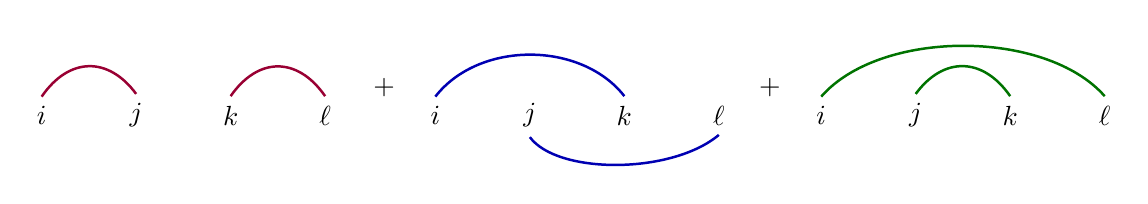
\begin{tikzpicture}[scale=1.0]
  \node (i) at (0,0) {$i$};
  \node (j) at (1.2,0) {$j$};
  \node (k) at (2.4,0) {$k$};
  \node (l) at (3.6,0) {$\ell$};
  \draw[purple!80!black,line width=0.9pt]
    (i.north) .. controls (0.35,0.75) and (0.85,0.75) .. (j.north);
  \draw[purple!80!black,line width=0.9pt]
    (k.north) .. controls (2.75,0.75) and (3.25,0.75) .. (l.north);
  \node at (4.35,0.35) {$+$};
  \node (i2) at (5.0,0) {$i$};
  \node (j2) at (6.2,0) {$j$};
  \node (k2) at (7.4,0) {$k$};
  \node (l2) at (8.6,0) {$\ell$};
  \draw[blue!70!black,line width=0.9pt]
    (i2.north) .. controls (5.55,0.95) and (6.85,0.95) .. (k2.north);
  \draw[blue!70!black,line width=0.9pt]
    (j2.south) .. controls (6.55,-0.75) and (8.0,-0.75) .. (l2.south);
  \node at (9.25,0.35) {$+$};
  \node (i3) at (9.9,0) {$i$};
  \node (j3) at (11.1,0) {$j$};
  \node (k3) at (12.3,0) {$k$};
  \node (l3) at (13.5,0) {$\ell$};
  \draw[green!45!black,line width=0.9pt]
    (i3.north) .. controls (10.65,1.1) and (12.75,1.1) .. (l3.north);
  \draw[green!45!black,line width=0.9pt]
    (j3.north) .. controls (11.45,0.75) and (11.95,0.75) .. (k3.north);
\end{tikzpicture}
\end{center}

A Wick contraction is an assigned pairing of two labels with value
\[
  (q_iq_j)_{\mathrm{contr}}=(A^{-1})_{ij}.
\]
Wick's theorem says that the Gaussian expectation of \(2r\) variables is the
sum over all complete pairings, with one covariance factor for each pair:
\[
  \langle q_{i_1}\cdots q_{i_{2r}}\rangle_A
  =
  \sum_{\text{complete pairings }P}
  \prod_{(a,b)\in P}(A^{-1})_{i_ai_b}.
\]
Gaussian expectations of an odd number of variables vanish.

\section{Gaussian Functional Integrals}

Let \(A\) be the positive operator
\[
  A=-\frac{\dd^2}{\dd\tau^2}+\omega^2
\]
on a function space with boundary conditions for which \(A\) is invertible.
The Green function \(G(\tau,\tau')\) is the integral kernel of \(A^{-1}\):
\[
  (A^{-1}f)(\tau)
  =
  \int G(\tau,\tau')f(\tau')\,\dd\tau',
\]
and therefore satisfies
\[
  \left(
    -\frac{\dd^2}{\dd\tau^2}+\omega^2
  \right)G(\tau,\tau')
  =
  \delta(\tau-\tau').
\]
With the inner product
\[
  (f,g)=\int f(\tau)g(\tau)\,\dd\tau,
\]
the Gaussian Euclidean action is
\[
  S_0[q]=\frac12(q,Aq).
\]
The source-dependent Gaussian functional integral is defined by a regulator,
for instance a finite-mode cutoff, and has the finite-dimensional form in the
cutoff variables. Its continuum notation is
\[
  Z_0[J]
  =
  \int[Dq]\,
  \exp\left[
    -\frac12(q,Aq)+(J,q)
  \right].
\]
The ratio independent of normalization is
\[
  \frac{Z_0[J]}{Z_0[0]}
  =
  \exp\left[
    \frac12\int J(\tau)G(\tau,\tau')J(\tau')\,
    \dd\tau\,\dd\tau'
  \right].
\]
Consequently
\[
  \langle q(\tau_1)q(\tau_2)\rangle_0
  =
  G(\tau_1,\tau_2).
\]

On the infinite Euclidean line, write
\[
  q(\tau)=
  \int_{-\infty}^{\infty}\frac{\dd k}{2\pi}\,
  \widetilde q(k)\ee^{\ii k\tau},
  \qquad
  \widetilde q(k)^*=\widetilde q(-k).
\]
Then
\[
  S_0[q]
  =
  \frac12
  \int_{-\infty}^{\infty}\frac{\dd k}{2\pi}\,
  \widetilde q(-k)(k^2+\omega^2)\widetilde q(k),
\]
and
\[
  \langle \widetilde q(k_1)\widetilde q(k_2)\rangle_0
  =
  \frac{2\pi\delta(k_1+k_2)}{k_1^2+\omega^2}.
\]
Thus
\[
  G(\tau,\tau')
  =
  \int_{-\infty}^{\infty}
  \frac{\dd k}{2\pi}\,
  \frac{\ee^{\ii k(\tau-\tau')}}{k^2+\omega^2}
  =
  \frac{1}{2\omega}\ee^{-\omega|\tau-\tau'|}.
\]

\section{The Anharmonic Oscillator}

Set \(\omega=1\) in this section. The anharmonic oscillator is defined by
\[
  \widehat H
  =
  \frac12\widehat p^2+\frac12\widehat q^2+\frac{g}{4!}\widehat q^4.
\]
The Euclidean Lagrangian is
\[
  L_E(q,q')
  =
  \frac12(q')^2+\frac12q^2+\frac{g}{4!}q^4.
\]
Let
\[
  S_0[q]=\int\left[\frac12(q')^2+\frac12q^2\right]\dd\tau,
  \qquad
  S_{\mathrm{int}}[q]=\frac{g}{4!}\int q(\tau)^4\,\dd\tau .
\]
At finite cutoff, perturbation theory is the expansion of
\(\exp[-S_{\mathrm{int}}]\) inside a finite-dimensional Gaussian integral.
For the partition function,
\[
  Z_g=\int[Dq]\,\exp[-S_0[q]-S_{\mathrm{int}}[q]],
\]
one obtains
\[
  \frac{Z_g}{Z_0}
  =
  \sum_{n=0}^{\infty}
  \frac{1}{n!}
  \left(-\frac{g}{4!}\right)^n
  \int \dd\tau_1\cdots\dd\tau_n\,
  \left\langle
    q(\tau_1)^4\cdots q(\tau_n)^4
  \right\rangle_0 .
\]
Here \(Z_0\) is the Gaussian partition function and
\(\langle\cdots\rangle_0\) is evaluated with
\[
  G_0(\tau,\tau')=\frac12\ee^{-|\tau-\tau'|}.
\]

At first order in \(g\),
\[
  -\frac{g}{4!}\int\dd\tau\,\langle q(\tau)^4\rangle_0
  =
  -\frac{g}{8}\int\dd\tau\,G_0(\tau,\tau)^2.
\]
The factor \(3\) in \(\langle q^4\rangle_0=3G_0(\tau,\tau)^2\) is the number
of pairings of four fields at the vertex.

\begin{center}
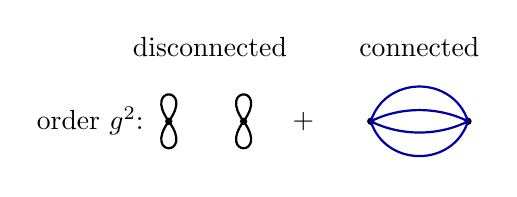
\begin{tikzpicture}[scale=0.95]
  \node at (-1.2,0) {order \(g^2\):};
  \node at (0.4,1.0) {disconnected};
  \foreach \x in {-0.15,0.85} {
    \draw[thick] (\x,0) .. controls (\x-0.35,0.48) and (\x+0.35,0.48) .. (\x,0);
    \draw[thick] (\x,0) .. controls (\x-0.35,-0.48) and (\x+0.35,-0.48) .. (\x,0);
    \fill (\x,0) circle (1.4pt);
  }
  \node at (1.65,0) {$+$};
  \node at (3.2,1.0) {connected};
  \foreach \x in {2.55,3.85} {
    \fill (\x,0) circle (1.4pt);
  }
  \draw[thick,blue!65!black]
    (2.55,0) .. controls (2.75,0.62) and (3.65,0.62) .. (3.85,0);
  \draw[thick,blue!65!black]
    (2.55,0) .. controls (2.75,-0.62) and (3.65,-0.62) .. (3.85,0);
  \draw[thick,blue!65!black]
    (2.55,0) .. controls (2.95,0.2) and (3.45,0.2) .. (3.85,0);
  \draw[thick,blue!65!black]
    (2.55,0) .. controls (2.95,-0.2) and (3.45,-0.2) .. (3.85,0);
\end{tikzpicture}
\end{center}

Let \(G^{(\ell)}\) be the sum of connected vacuum Wick contractions involving
\(\ell\) interaction vertices, including the coupling factors and integration
over the \(\ell\) vertex positions. If \(m_\ell\) is the number of connected
components of size \(\ell\), then
\[
  \sum_{\ell\ge1}\ell\,m_\ell=n.
\]
The number of ways to partition \(n\) labelled vertices into this pattern is
\[
  \frac{n!}{\prod_{\ell\ge1}(\ell!)^{m_\ell}m_\ell!}.
\]
Summing over all patterns gives the linked-cluster formula
\[
  \frac{Z_g}{Z_0}
  =
  \exp\left[
    \sum_{\ell\ge1}\frac{1}{\ell!}G^{(\ell)}
  \right].
\]
Equivalently, \(\log Z_g\) is the sum of connected vacuum diagrams.

On a long interval of Euclidean length \(T_{\mathrm{tot}}\),
\[
  Z_g\sim \exp[-E_0(g)T_{\mathrm{tot}}],
\]
up to endpoint factors. Hence
\[
  E_0(g)
  =
  -\lim_{T_{\mathrm{tot}}\to\infty}
  \frac{1}{T_{\mathrm{tot}}}\log Z_g.
\]
The first correction is
\[
  \Delta E_0
  =
  \frac{g}{8}G_0(0)^2+O(g^2)
  =
  \frac{g}{32}+O(g^2),
\]
in agreement with first-order Hamiltonian perturbation theory:
\[
  \bra{\psi_0}\frac{g}{4!}\widehat q^4\ket{\psi_0}
  =
  \frac{g}{4!}\,3\left(\frac12\right)^2
  =
  \frac{g}{32}.
\]

\section{Connected Two-Point Functions and Self-Energy}

The normalized Euclidean two-point function is
\[
  G(\tau)
  =
  \langle q(\tau)q(0)\rangle_g
  =
  \frac{1}{Z_g}
  \int[Dq]\,\ee^{-S_0[q]-S_{\mathrm{int}}[q]}\,q(\tau)q(0).
\]
In the perturbative expansion, every Wick contraction splits uniquely into
the connected component containing the two external insertions and a product
of vacuum components. The sum of the vacuum components is \(Z_g\), and is
cancelled by the normalization. Thus \(G(\tau)\) is the sum of connected
two-point diagrams.

\begin{center}
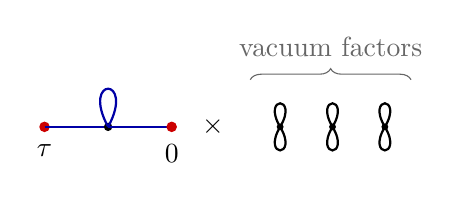
\begin{tikzpicture}[scale=0.95]
  \fill[red!80!black] (0,0) circle (2pt);
  \node[below=3pt] at (0,0) {$\tau$};
  \draw[thick,blue!65!black] (0,0) -- (0.85,0);
  \fill (0.85,0) circle (1.6pt);
  \draw[thick,blue!65!black]
    (0.85,0) .. controls (0.48,0.68) and (1.22,0.68) .. (0.85,0);
  \draw[thick,blue!65!black] (0.85,0) -- (1.7,0);
  \fill[red!80!black] (1.7,0) circle (2pt);
  \node[below=3pt] at (1.7,0) {$0$};
  \node at (2.25,0) {$\times$};
  \draw[decorate,decoration={brace,amplitude=4pt},gray!80!black]
    (2.75,0.63) -- node[midway,above=5pt] {vacuum factors} (4.9,0.63);
  \foreach \x in {3.15,3.85,4.55} {
    \draw[thick] (\x,0) .. controls (\x-0.25,0.42) and (\x+0.25,0.42) .. (\x,0);
    \draw[thick] (\x,0) .. controls (\x-0.25,-0.42) and (\x+0.25,-0.42) .. (\x,0);
    \fill (\x,0) circle (1.3pt);
  }
\end{tikzpicture}
\end{center}

At zeroth order,
\[
  G_0(\tau)=\frac12\ee^{-|\tau|}
  =
  \int_{-\infty}^{\infty}\frac{\dd k}{2\pi}\,
  \frac{\ee^{\ii k\tau}}{k^2+1}.
\]
At order \(g\), the connected tadpole correction is
\[
  -\frac{g}{2}
  \int \dd\tau'\,
  G_0(\tau-\tau')G_0(\tau')G_0(0).
\]
In momentum space this becomes
\[
  -\frac{g}{4}
  \int_{-\infty}^{\infty}\frac{\dd k}{2\pi}\,
  \frac{\ee^{\ii k\tau}}{(k^2+1)^2}.
\]

A connected two-point diagram is one-particle-irreducible, abbreviated
\(1\mathrm{PI}\), when it remains connected after cutting any one internal
propagator. In this chapter the term is graph-theoretic and refers to
Euclidean Green-function diagrams. Let \(\Sigma(k)\) be the sum of amputated
\(1\mathrm{PI}\) two-point insertions in momentum space. Then the full
two-point function is the geometric series
\[
  \widetilde G(k)
  =
  \widetilde G_0(k)
  \sum_{r=0}^{\infty}
  \bigl(\widetilde G_0(k)\Sigma(k)\bigr)^r
  =
  \frac{1}{k^2+1-\Sigma(k)},
  \qquad
  \widetilde G_0(k)=\frac{1}{k^2+1}.
\]

\begin{center}
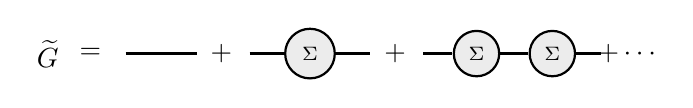
\begin{tikzpicture}[scale=0.9]
  \node at (-0.55,0) {$\widetilde G$};
  \node at (0.05,0) {$=$};
  \draw[thick] (0.55,0) -- (1.55,0);
  \node at (1.9,0) {$+$};
  \draw[thick] (2.3,0) -- (2.8,0);
  \draw[thick,fill=gray!15] (3.15,0) circle (0.35);
  \node at (3.15,0) {\scriptsize \(\Sigma\)};
  \draw[thick] (3.5,0) -- (4.0,0);
  \node at (4.35,0) {$+$};
  \draw[thick] (4.75,0) -- (5.15,0);
  \draw[thick,fill=gray!15] (5.5,0) circle (0.32);
  \node at (5.5,0) {\scriptsize \(\Sigma\)};
  \draw[thick] (5.82,0) -- (6.22,0);
  \draw[thick,fill=gray!15] (6.57,0) circle (0.32);
  \node at (6.57,0) {\scriptsize \(\Sigma\)};
  \draw[thick] (6.89,0) -- (7.25,0);
  \node at (7.62,0) {$+\cdots$};
\end{tikzpicture}
\end{center}

For the anharmonic oscillator,
\[
  \Sigma(k)
  =
  -\frac{g}{4}
  +
  \frac{g^2}{8}
  \left(
    \frac14+\frac{1}{k^2+9}
  \right)
  +O(g^3).
\]
The spectral expansion says that for \(\tau>0\),
\[
  G(\tau)
  =
  \sum_n
  \left|\bra n\widehat q\ket 0\right|^2
  \ee^{-(E_n-E_0)\tau}.
\]
The Fourier representation
\[
  G(\tau)
  =
  \int_{-\infty}^{\infty}\frac{\dd k}{2\pi}\,
  \widetilde G(k)\ee^{\ii k\tau}
\]
is evaluated by closing the contour in the upper half-plane. If
\(\widetilde G(k)\) has simple poles at \(k=\ii\omega_n\), then
\[
  G(\tau)
  =
  \ii\sum_n
  \operatorname*{Res}_{k=\ii\omega_n}\widetilde G(k)\,
  \ee^{-\omega_n\tau}.
\]
Thus the pole positions encode the energy gaps \(\omega_n=E_n-E_0\) in the
\(\hbar=1\) convention. The pole near \(k=\ii\) gives
\[
  E_1-E_0
  =
  1+\frac{g}{8}-\frac{g^2}{32}+O(g^3).
\]

\section{Derivative Interactions, Regulators, and Counterterms}

Consider the Lagrangian
\[
  L(q,\dot q)
  =
  \frac12\dot q^2-\frac12q^2-\frac{g}{8}q^2\dot q^2 .
\]
The canonical momentum is
\[
  p=\frac{\partial L}{\partial\dot q}
  =
  \dot q\left(1-\frac{g}{4}q^2\right),
\]
and the corresponding Hamiltonian function is
\[
  H(q,p)
  =
  \frac12\left(1-\frac{g}{4}q^2\right)^{-1}p^2
  +\frac12q^2.
\]
The Euclidean Lagrangian is
\[
  L_E(q,q')
  =
  \frac12(q')^2+\frac12q^2-\frac{g}{8}q^2(q')^2 .
\]
Using
\[
  q^2(q')^2
  =
  \frac13\frac{\dd}{\dd\tau}(q^3q')
  -\frac13q^3q'',
\]
the interaction may also be represented, up to endpoint terms, by
\[
  \frac{g}{24}q^3q''.
\]

At first order in \(g\), the two-point function contains contractions in
which derivatives act on propagators at coincident points. A representative
term is
\[
  \frac{g}{4}\int\dd\tau'\,
  G_0(\tau-\tau')G_0(\tau')\,
  \bigl[-\partial_{\tau'}^2G_0(\tau'-\tau')\bigr].
\]
In momentum space this contains
\[
  \int\frac{\dd k'}{2\pi}\frac{k'^2}{k'^2+1},
\]
which depends on the high-frequency definition of the path integral.

\begin{center}
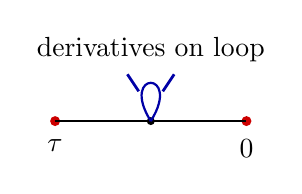
\begin{tikzpicture}[scale=0.9]
  \coordinate (a) at (0,0);
  \coordinate (b) at (1.35,0);
  \coordinate (c) at (2.7,0);
  \fill[red!80!black] (a) circle (2pt);
  \node[below=3pt] at (a) {$\tau$};
  \fill[red!80!black] (c) circle (2pt);
  \node[below=3pt] at (c) {$0$};
  \fill (b) circle (1.6pt);
  \draw[thick] (a) -- (b) -- (c);
  \draw[thick,blue!65!black]
    (b) .. controls (0.9,0.72) and (1.8,0.72) .. (b);
  \draw[blue!65!black,line width=1pt] (1.18,0.42) -- (1.02,0.66);
  \draw[blue!65!black,line width=1pt] (1.52,0.42) -- (1.68,0.66);
  \node[above=18pt] at (b) {derivatives on loop};
\end{tikzpicture}
\end{center}

Define a frequency cutoff by
\[
  q(\tau)
  =
  \int_{|k|<\Lambda}\frac{\dd k}{2\pi}\,
  \widetilde q(k)\ee^{\ii k\tau},
  \qquad
  [Dq]_\Lambda=\prod_{|k|<\Lambda}\dd \widetilde q(k),
\]
with the real-field condition \(\widetilde q(k)^*=\widetilde q(-k)\). After
restoring \(\hbar\), the first-order self-energy has the form
\[
  \Sigma_\Lambda(k)
  =
  \frac{\hbar g}{4}
  \left(
    \frac{\Lambda}{\pi}
    +\frac{k^2}{2}
    -\frac12
    +O(\Lambda^{-1})
  \right)
  +O(\hbar^2g^2).
\]
A local Euclidean counterterm
\[
  \Delta L_E=C\,g\,\hbar\,\frac{q^2}{2}
\]
adds \(-Cg\hbar\) to \(\Sigma_\Lambda(k)\), so that
\[
  \Sigma_\Lambda(k)
  =
  \hbar g
  \left(
    \frac{k^2}{8}
    +\frac{\Lambda}{4\pi}
    -\frac18
    -C
    +O(\Lambda^{-1})
  \right)
  +O(g^2).
\]
Choosing
\[
  C=\frac{\Lambda}{4\pi}+C_{\mathrm{fin}}
\]
defines a finite limiting two-point function as \(\Lambda\to\infty\). The
finite constant \(C_{\mathrm{fin}}\) is part of the quantum definition of the
Hamiltonian represented by this regulated Lagrangian path integral.

The structural statement carried forward to field theory is this: a path
integral with interactions is a regulated construction of Green functions,
and local counterterms are part of the data specifying the regulated
construction and its limiting prescription. The next chapter replaces the
single coordinate \(q(\tau)\) by fields \(\phi(x)\) and imposes relativistic
covariance and locality on the resulting Green functions.

\chapter{Relativistic Scalar Fields and Canonical Quantization}
\label{ch:relativistic-scalar-fields-canonical-quantization}
\ConventionsLorentzian


\section{Fields and Variational Equations}

Let \(\mathbb M^D\) be \(D\)-dimensional Minkowski spacetime with metric
\[
  \eta_{\mu\nu}=\operatorname{diag}(-1,+1,\ldots,+1).
\]
Write
\[
  x^\mu=(x^0,\vec x),\qquad x^0=t,\qquad \vec x\in\mathbb R^{D-1}.
\]
A real classical scalar field is a real-valued function
\[
  \phi:\mathbb M^D\to\mathbb R.
\]
The field-theoretic analogue of finitely many coordinates \(q^i(t)\) is the
family of coordinates \(\phi(t,\vec x)\), labelled continuously by
\(\vec x\). A Lagrangian field theory is specified by an action functional
\[
  S[\phi]
  =
  \int_{\mathbb M^D}\dd^D x\,
  \mathcal L\bigl(\phi(x),\partial_\mu\phi(x)\bigr),
\]
where \(\mathcal L\) is a Lorentz scalar Lagrangian density in the examples
below.

For a compactly supported variation \(\delta\phi\),
\[
\begin{aligned}
  \delta S
  &=
  \int\dd^Dx\,
  \left[
    \frac{\partial\mathcal L}{\partial\phi}\,\delta\phi
    +
    \frac{\partial\mathcal L}
         {\partial(\partial_\mu\phi)}
    \,\partial_\mu\delta\phi
  \right]  \\
  &=
  \int\dd^Dx\,\delta\phi
  \left[
    \frac{\partial\mathcal L}{\partial\phi}
    -
    \partial_\mu
    \frac{\partial\mathcal L}
         {\partial(\partial_\mu\phi)}
  \right].
\end{aligned}
\]
The Euler--Lagrange equation is therefore
\[
  \frac{\partial\mathcal L}{\partial\phi}
  -
  \partial_\mu
  \frac{\partial\mathcal L}{\partial(\partial_\mu\phi)}
  =
  0.
\]

\section{The Free Massive Scalar}

The free massive real scalar field of mass \(m\ge0\) has Lagrangian density
\[
  \mathcal L
  =
  \frac12(\partial_t\phi)^2
  -\frac12\sum_{i=1}^{D-1}(\partial_i\phi)^2
  -\frac12m^2\phi^2.
\]
Equivalently,
\[
  \mathcal L
  =
  -\frac12\partial_\mu\phi\,\partial^\mu\phi
  -\frac12m^2\phi^2,
  \qquad
  \partial^\mu=\eta^{\mu\nu}\partial_\nu.
\]
The Euler--Lagrange equation is the Klein--Gordon equation
\[
  (\partial^\mu\partial_\mu-m^2)\phi=0.
\]

Use the Fourier convention
\[
  \phi(x)
  =
  \int\frac{\dd^Dk}{(2\pi)^D}\,
  \widetilde\phi(k)\,\ee^{\ii k\cdot x},
  \qquad
  k\cdot x=\eta_{\mu\nu}k^\mu x^\nu
  =
  -k^0x^0+\vec k\cdot\vec x.
\]
The equation of motion implies
\[
  (k^2+m^2)\widetilde\phi(k)=0,
  \qquad
  k^2=\eta_{\mu\nu}k^\mu k^\nu.
\]
Thus \(\widetilde\phi(k)\) is supported on the mass shell
\[
  k^2+m^2=0,
  \qquad
  k^0=\pm\omega_{\vec k},
  \qquad
  \omega_{\vec k}=\sqrt{\vec k^{\,2}+m^2}.
\]

\begin{center}
\begin{tikzpicture}[>=Stealth,scale=0.95]
  \draw[->] (-3.15,0) -- (3.35,0) node[right] {$|\vec k|$};
  \draw[->] (0,-2.55) -- (0,2.75) node[above] {$k^0$};
  \draw[blue!70!black,line width=1pt,domain=-2.65:2.65,samples=100]
    plot (\x,{sqrt(0.65+\x*\x)});
  \draw[blue!70!black,line width=1pt,domain=-2.65:2.65,samples=100]
    plot (\x,{-sqrt(0.65+\x*\x)});
  \node[blue!70!black,right] at (2.05,2.25) {$k^0=+\omega_{\vec k}$};
  \node[blue!70!black,right] at (2.05,-2.25) {$k^0=-\omega_{\vec k}$};
  \node at (-1.25,0.35) {$k^2+m^2=0$};
\end{tikzpicture}
\end{center}

A real solution can be written as
\[
  \phi(t,\vec x)
  =
  \int\frac{\dd^{D-1}\vec k}{(2\pi)^{D-1}}
  \left[
    A(\vec k)\,\ee^{\ii\vec k\cdot\vec x-\ii\omega_{\vec k}t}
    +
    A(\vec k)^*\,\ee^{-\ii\vec k\cdot\vec x+\ii\omega_{\vec k}t}
  \right],
\]
with a complex coefficient function \(A(\vec k)\) subject to whatever
regularity conditions are imposed on the classical solution. The Cauchy data
\[
  \phi(0,\vec x),\qquad \partial_t\phi(0,\vec x)
\]
determine \(A(\vec k)\) and \(A(\vec k)^*\), hence determine the free
solution for all \(t\). Explicitly, write
\[
  \phi(0,\vec x)
  =
  \int\frac{\dd^{D-1}\vec k}{(2\pi)^{D-1}}\,
  \widetilde\phi_0(\vec k)\ee^{\ii\vec k\cdot\vec x},
  \qquad
  \partial_t\phi(0,\vec x)
  =
  \int\frac{\dd^{D-1}\vec k}{(2\pi)^{D-1}}\,
  \widetilde\pi_0(\vec k)\ee^{\ii\vec k\cdot\vec x}.
\]
Then
\[
  \widetilde\phi_0(\vec k)
  =
  A(\vec k)+A(-\vec k)^*,
  \qquad
  \widetilde\pi_0(\vec k)
  =
  -\ii\omega_{\vec k}\bigl(A(\vec k)-A(-\vec k)^*\bigr),
\]
so that
\[
  A(\vec k)
  =
  \frac12\left(
    \widetilde\phi_0(\vec k)
    +
    \frac{\ii}{\omega_{\vec k}}\widetilde\pi_0(\vec k)
  \right).
\]

There are two constructions to keep distinct. Canonical quantization starts
from the equal-time phase space \((\phi,\Pi)\) and a Hamiltonian. The
Lagrangian path-integral construction is defined by first choosing a regulator
that replaces the field by finitely many coordinates or modes:
\[
  \int_{\mathcal C_R}\dd\mu_R(\phi_R)\,
  \exp\left(\frac{\ii}{\hbar}S_R[\phi_R]\right).
\]
Here \(R\) labels the chosen cutoff, \(\mathcal C_R\) is the regulated
configuration space, \(\dd\mu_R\) is the corresponding finite-dimensional or
lattice measure, and \(S_R\) is the regulated action.  The continuum symbol
\(\int[D\phi]\exp(\ii S[\phi]/\hbar)\) denotes a specified limit or asymptotic
expansion of these regulated objects. This chapter develops the canonical
construction; the scalar field path integral is introduced later.

\section{Canonical Hamiltonian Formalism}

Let
\[
  L(t)=\int\dd^{D-1}\vec x\,\mathcal L.
\]
The canonical momentum density conjugate to \(\phi(t,\vec x)\) is
\[
  \Pi(t,\vec x)
  =
  \frac{\partial\mathcal L}
       {\partial(\partial_t\phi(t,\vec x))}.
\]
For the free scalar,
\[
  \Pi(t,\vec x)=\partial_t\phi(t,\vec x).
\]
The Hamiltonian density is
\[
  \mathcal H
  =
  \Pi\,\partial_t\phi-\mathcal L,
\]
and therefore
\[
  \mathcal H
  =
  \frac12\Pi^2
  +
  \frac12\sum_{i=1}^{D-1}(\partial_i\phi)^2
  +
  \frac12m^2\phi^2
\]
for the free scalar field. The Hamiltonian is
\[
  H=\int\dd^{D-1}\vec x\,\mathcal H.
\]

For functionals \(F[\phi,\Pi]\) and \(G[\phi,\Pi]\), use the equal-time
Poisson bracket
\[
  \{F,G\}
  =
  \int\dd^{D-1}\vec x
  \left[
    \frac{\delta F}{\delta\phi(\vec x)}
    \frac{\delta G}{\delta\Pi(\vec x)}
    -
    \frac{\delta F}{\delta\Pi(\vec x)}
    \frac{\delta G}{\delta\phi(\vec x)}
  \right].
\]
Then
\[
  \{\phi(\vec x),\Pi(\vec y)\}
  =
  \delta^{(D-1)}(\vec x-\vec y),
\]
with the \(\phi\)-\(\phi\) and \(\Pi\)-\(\Pi\) brackets equal to zero. Hamilton's
equation is
\[
  \partial_tF=\{F,H\}.
\]
Applied to \(\phi\) and \(\Pi\), it reproduces the Klein--Gordon equation.

\section{Equal-Time Quantization}

Canonical quantization promotes the classical fields to operator-valued
distributions
\[
  \widehat\phi(t,\vec x),\qquad \widehat\Pi(t,\vec x)
\]
on a common dense domain. Their equal-time commutation relations are
\[
  [\widehat\phi(t,\vec x),\widehat\Pi(t,\vec y)]
  =
  \ii\hbar\,\delta^{(D-1)}(\vec x-\vec y),
\]
and
\[
  [\widehat\phi(t,\vec x),\widehat\phi(t,\vec y)]
  =
  0
  =
  [\widehat\Pi(t,\vec x),\widehat\Pi(t,\vec y)].
\]
All pointwise products are distributional notation. Smeared fields, for
test functions \(f,g\in C_c^\infty(\mathbb R^{D-1})\), are
\[
  \widehat\phi_t(f)=\int\dd^{D-1}\vec x\,f(\vec x)\widehat\phi(t,\vec x),
  \qquad
  \widehat\Pi_t(g)=\int\dd^{D-1}\vec x\,g(\vec x)\widehat\Pi(t,\vec x).
\]
The smeared commutator is
\[
  [\widehat\phi_t(f),\widehat\Pi_t(g)]
  =
  \ii\hbar
  \int\dd^{D-1}\vec x\,f(\vec x)g(\vec x).
\]

For the rest of this chapter set \(\hbar=1\). With \(\hbar\) retained, the
oscillator algebra below reads
\[
  [b_{\vec k},b^\dagger_{\vec q}]
  =
  \hbar(2\pi)^{D-1}\delta^{(D-1)}(\vec k-\vec q).
\]
Equivalently, the \(\hbar=1\) variables are obtained from the \(\hbar\)-full
variables by \(b_{\vec k}^{(\hbar=1)}=\hbar^{-1/2}b_{\vec k}^{(\hbar)}\).

\section{Oscillator Variables and the Hamiltonian}

Let \(\nu_{\vec k}>0\) be a positive even function of \(\vec k\). Define
operator-valued distributions \(b_{\vec k}\) and \(b^\dagger_{\vec k}\) by the
equal-time expansion
\[
  \widehat\phi(0,\vec x)
  =
  \int\frac{\dd^{D-1}\vec k}{(2\pi)^{D-1}}\,
  \frac{1}{\sqrt{2\nu_{\vec k}}}
  \left(
    b_{\vec k}\ee^{\ii\vec k\cdot\vec x}
    +
    b^\dagger_{\vec k}\ee^{-\ii\vec k\cdot\vec x}
  \right),
\]
\[
  \widehat\Pi(0,\vec x)
  =
  \int\frac{\dd^{D-1}\vec k}{(2\pi)^{D-1}}\,
  (-\ii)\sqrt{\frac{\nu_{\vec k}}{2}}
  \left(
    b_{\vec k}\ee^{\ii\vec k\cdot\vec x}
    -
    b^\dagger_{\vec k}\ee^{-\ii\vec k\cdot\vec x}
  \right).
\]
The equal-time commutation relations are equivalent to
\[
  [b_{\vec k},b_{\vec q}]=0
  =
  [b^\dagger_{\vec k},b^\dagger_{\vec q}],
  \qquad
  [b_{\vec k},b^\dagger_{\vec q}]
  =
  (2\pi)^{D-1}\delta^{(D-1)}(\vec k-\vec q).
\]
This algebra holds for every positive choice of \(\nu_{\vec k}\). The
notation \(b_{\vec k}\), \(b^\dagger_{\vec k}\) should therefore not yet be
read as a particle interpretation. If \(\lambda_{\vec k}>0\) is another even
function, define \(c_{\vec k}\), \(c^\dagger_{\vec k}\) by
\[
  c_{\vec k}+c^\dagger_{-\vec k}
  =
  \lambda_{\vec k}\bigl(b_{\vec k}+b^\dagger_{-\vec k}\bigr),
  \qquad
  c_{\vec k}-c^\dagger_{-\vec k}
  =
  \lambda_{\vec k}^{-1}\bigl(b_{\vec k}-b^\dagger_{-\vec k}\bigr).
\]
Equivalently,
\[
  c_{\vec k}
  =
  \frac{\lambda_{\vec k}+\lambda_{\vec k}^{-1}}{2}\,b_{\vec k}
  +
  \frac{\lambda_{\vec k}-\lambda_{\vec k}^{-1}}{2}\,
  b^\dagger_{-\vec k}.
\]
The \(c\)'s obey the same canonical oscillator algebra. If a vector is
annihilated by every \(b_{\vec k}\), it is not annihilated by every
\(c_{\vec k}\) unless \(\lambda_{\vec k}=1\). The Hamiltonian is the datum
that selects the oscillator normalization.

Let
\[
  \omega_{\vec k}=\sqrt{\vec k^{\,2}+m^2}.
\]
Substituting the mode expansion into the free Hamiltonian gives
\[
\begin{aligned}
  \widehat H_0
  =
  \int\frac{\dd^{D-1}\vec k}{(2\pi)^{D-1}}
  \Bigg[
  &\frac{\nu_{\vec k}^2+\omega_{\vec k}^2}{2\nu_{\vec k}}
  \left(
    b^\dagger_{\vec k}b_{\vec k}
    +\frac12(2\pi)^{D-1}\delta^{(D-1)}(0)
  \right)\\
  &+
  \frac{\omega_{\vec k}^2-\nu_{\vec k}^2}{4\nu_{\vec k}}
  \left(
    b_{\vec k}b_{-\vec k}
    +
    b^\dagger_{\vec k}b^\dagger_{-\vec k}
  \right)
  \Bigg].
\end{aligned}
\]
The off-diagonal terms vanish precisely for
\[
  \nu_{\vec k}=\omega_{\vec k}.
\]
With this choice,
\[
  \widehat H_0
  =
  \int\frac{\dd^{D-1}\vec k}{(2\pi)^{D-1}}\,
  \omega_{\vec k}
  \left(
    b^\dagger_{\vec k}b_{\vec k}
    +\frac12(2\pi)^{D-1}\delta^{(D-1)}(0)
  \right).
\]
At finite spatial volume and finite momentum cutoff, the second term is a
finite scalar multiple of the identity. A constant multiple of the identity
does not change Heisenberg evolution, but the quantum Hamiltonian must be a
well-defined self-adjoint operator after the regulator is removed. We
therefore choose the additive energy normalization so that the invariant
vacuum has zero energy. With this normalization the free Hamiltonian is
\[
  \widehat H_0^{\mathrm{ren}}
  =
  \int\frac{\dd^{D-1}\vec k}{(2\pi)^{D-1}}\,
  \omega_{\vec k} b^\dagger_{\vec k}b_{\vec k}.
\]
The free vacuum \(\vac\) is defined by
\[
  b_{\vec k}\vac=0
  \qquad\text{for all }\vec k,
\]
and satisfies \(\widehat H_0^{\mathrm{ren}}\vac=0\).

Time evolution generated by \(\widehat H_0^{\mathrm{ren}}\) gives
\[
  \widehat\phi(x)
  =
  \int\frac{\dd^{D-1}\vec k}{(2\pi)^{D-1}}\,
  \frac{1}{\sqrt{2\omega_{\vec k}}}
  \left(
    b_{\vec k}\ee^{\ii\vec k\cdot\vec x-\ii\omega_{\vec k}t}
    +
    b^\dagger_{\vec k}\ee^{-\ii\vec k\cdot\vec x+\ii\omega_{\vec k}t}
  \right).
\]

The invariant mass-shell normalization used earlier is obtained by defining
\[
  a(\vec k)=\sqrt{2\omega_{\vec k}}\,b_{\vec k},
  \qquad
  a^\dagger(\vec k)=\sqrt{2\omega_{\vec k}}\,b^\dagger_{\vec k}.
\]
Then
\[
  [a(\vec k),a^\dagger(\vec q)]
  =
  (2\pi)^{D-1}2\omega_{\vec k}\,
  \delta^{(D-1)}(\vec k-\vec q),
\]
and
\[
  \widehat\phi(x)
  =
  \int
  \frac{\dd^{D-1}\vec k}{(2\pi)^{D-1}2\omega_{\vec k}}\,
  \left(
    a(\vec k)\ee^{\ii k\cdot x}
    +
    a^\dagger(\vec k)\ee^{-\ii k\cdot x}
  \right),
  \qquad
  k^0=\omega_{\vec k}.
\]
This is the convention used for the free scalar field in the earlier
Fock-space construction.

\section{Covariance and Microcausality}

Let \(\mathcal D_0\) be the finite-particle domain generated by applying
finitely many smeared creation operators to \(\vac\). On \(\mathcal D_0\),
\(\widehat\phi(x)\) is an operator-valued distribution. For
\(f\in C_c^\infty(\mathbb M^D)\),
\[
  \widehat\phi(f)=\int\dd^D x\,f(x)\widehat\phi(x)
\]
is the corresponding smeared operator on \(\mathcal D_0\).

The free Fock representation carries the unitary Poincare representation
induced from the one-particle mass shell. With the above normalization, the
field transforms as a scalar:
\[
  U(a,\Lambda)^{-1}\widehat\phi(x)U(a,\Lambda)
  =
  \widehat\phi(\Lambda x+a).
\]

The commutator is
\[
  [\widehat\phi(x),\widehat\phi(y)]
  =
  \ii\,\Delta(x-y),
\]
where the Pauli--Jordan distribution is
\[
  \Delta(x)
  =
  \frac{1}{\ii}
  \int
  \frac{\dd^{D-1}\vec k}{(2\pi)^{D-1}2\omega_{\vec k}}
  \left(
    \ee^{\ii k\cdot x}
    -
    \ee^{-\ii k\cdot x}
  \right),
  \qquad k^0=\omega_{\vec k}.
\]
This distribution is Lorentz invariant. If \(x\) is spacelike, a Lorentz
transformation sends it to \((0,\vec r)\). At equal time,
\[
  \Delta(0,\vec r)
  =
  \frac{1}{\ii}
  \int
  \frac{\dd^{D-1}\vec k}{(2\pi)^{D-1}2\omega_{\vec k}}
  \left(
    \ee^{\ii\vec k\cdot\vec r}
    -
    \ee^{-\ii\vec k\cdot\vec r}
  \right)
  =
  0,
\]
because the two terms are exchanged by \(\vec k\mapsto-\vec k\). Therefore
\[
  [\widehat\phi(x),\widehat\phi(y)]=0
  \qquad
  \text{when }(x-y)^2>0.
\]
Equivalently,
\[
  [\widehat\phi(f),\widehat\phi(g)]=0
\]
when \(\operatorname{supp}f\) and \(\operatorname{supp}g\) are spacelike
separated. This verifies microcausality for the canonically quantized free
scalar field.

The next step in the construction is to identify the local currents and
charges attached to spacetime symmetries. That is the role of Noether's
theorem in the following chapter.

\chapter{Symmetries, Noether Currents, and Stress Tensors}
\label{ch:symmetries-noether-stress}
\ConventionsLorentzian


\section{Variational Framework}

\begin{definition}[First-derivative classical field datum]
\label{def:first-derivative-classical-field-datum}
Work on \(D\)-dimensional Minkowski spacetime \(\mathbb M^D\), with
mostly-plus metric \(\eta_{\mu\nu}\).  Let \(A\) range over a finite set of
bosonic field components.  A classical field configuration is a smooth map
\[
  \phi:M\longrightarrow \mathbb R^N,\qquad
  x\longmapsto \{\phi^A(x)\},
\]
on a spacetime region \(M\subset \mathbb M^D\).  In this chapter a Lagrangian
density means a first-derivative local expression
\[
  \mathcal L=\mathcal L(\phi^A,\partial_\mu\phi^A)
\]
with no dependence on derivatives of order two or higher.  The corresponding
action over \(M\) is
\[
  S_M[\phi]=\int_M\dd^Dx\,\mathcal L(\phi,\partial\phi).
\]
A variation is a smooth one-parameter family \(\phi_s\) with
\(\phi_0=\phi\); its tangent is
\[
  \delta\phi^A=\left.\frac{\dd}{\dd s}\phi_s^A\right|_{s=0}.
\]
When the boundary term is not part of the question, \(\delta\phi^A\) is
assumed to have compact support in \(M^\circ\), the interior of \(M\).
\end{definition}

\begin{proposition}[First variational identity]
\label{prop:first-variational-identity}
For the datum of
Definition~\ref{def:first-derivative-classical-field-datum}, define the
Euler--Lagrange expression
\[
  E_A(\mathcal L)
  =
  \frac{\partial\mathcal L}{\partial\phi^A}
  -
  \partial_\mu
  \frac{\partial\mathcal L}{\partial(\partial_\mu\phi^A)} .
\]
Then every smooth variation satisfies
\[
  \delta\mathcal L
  =
  E_A(\mathcal L)\,\delta\phi^A
  +
  \partial_\mu\theta^\mu(\delta\phi),
  \qquad
  \theta^\mu(\delta\phi)
  =
  \frac{\partial\mathcal L}{\partial(\partial_\mu\phi^A)}
  \delta\phi^A ,
\]
where repeated component and spacetime indices are summed.  Consequently
\[
  \delta S_M
  =
  \int_M\dd^Dx\,E_A(\mathcal L)\,\delta\phi^A
  +
  \int_{\partial M}\dd\Sigma_\mu\,\theta^\mu(\delta\phi),
\]
where \(\dd\Sigma_\mu\) is the oriented hypersurface measure on
\(\partial M\).
\end{proposition}

\begin{proof}
The chain rule gives
\[
  \delta\mathcal L
  =
  \frac{\partial\mathcal L}{\partial\phi^A}\delta\phi^A
  +
  \frac{\partial\mathcal L}{\partial(\partial_\mu\phi^A)}
  \partial_\mu\delta\phi^A .
\]
Apply the product rule to the second term:
\[
  \frac{\partial\mathcal L}{\partial(\partial_\mu\phi^A)}
  \partial_\mu\delta\phi^A
  =
  \partial_\mu
  \left(
    \frac{\partial\mathcal L}{\partial(\partial_\mu\phi^A)}
    \delta\phi^A
  \right)
  -
  \partial_\mu
  \frac{\partial\mathcal L}{\partial(\partial_\mu\phi^A)}
  \delta\phi^A .
\]
Combining the two non-divergence terms gives \(E_A(\mathcal L)\delta\phi^A\).
Integrating the pointwise identity over \(M\) and applying Stokes' theorem
gives the displayed formula for \(\delta S_M\).
\end{proof}

\begin{definition}[Classical solution]
\label{def:classical-solution-euler-lagrange}
A classical solution of the first-derivative Lagrangian problem is a field
configuration obeying
\[
  E_A(\mathcal L)=0
\]
for every component \(A\), together with the boundary or asymptotic conditions
specified by the variational problem.  The Euler--Lagrange equation alone is
not a complete boundary-value or Cauchy problem; the boundary data are part of
the definition of the classical problem being solved.
\end{definition}

\section{Infinitesimal Symmetries}

\begin{definition}[Infinitesimal variational symmetry]
\label{def:infinitesimal-variational-symmetry}
An infinitesimal field-space transformation is a rule
\[
  \delta_R\phi^A=R^A[\phi],
\]
where \(R^A[\phi]\) is a local expression in \(x\), the fields, and finitely
many derivatives of the fields.  The transformation is a variational symmetry
of the action if there exists a local vector \(K_R^\mu\) such that
\[
  \delta_R\mathcal L=\partial_\mu K_R^\mu .
\]
This equation is the definition of the symmetry in the present classical
Lagrangian framework.  It is an off-shell identity of local functions of the
fields; no Euler--Lagrange equation has yet been imposed.
\end{definition}

\begin{proposition}[Noether identity for a variational symmetry]
\label{prop:noether-identity-variational-symmetry}
Let \(R\) be a variational symmetry in the sense of
Definition~\ref{def:infinitesimal-variational-symmetry}.  The local current
\[
  j_R^\mu
  =
  \frac{\partial\mathcal L}{\partial(\partial_\mu\phi^A)}R^A
  -
  K_R^\mu
\]
obeys the off-shell identity
\[
  E_A(\mathcal L)R^A+\partial_\mu j_R^\mu=0.
\]
In particular, on every classical solution,
\[
  \partial_\mu j_R^\mu=0 .
\]
\end{proposition}

\begin{proof}
Apply Proposition~\ref{prop:first-variational-identity} to the variation
\(\delta_R\phi^A=R^A\):
\[
  \delta_R\mathcal L
  =
  E_A(\mathcal L)R^A
  +
  \partial_\mu
  \left(
    \frac{\partial\mathcal L}{\partial(\partial_\mu\phi^A)}R^A
  \right).
\]
The variational-symmetry condition says that the left hand side is
\(\partial_\mu K_R^\mu\).  Moving this total derivative to the right gives the
displayed off-shell identity.  Setting \(E_A(\mathcal L)=0\) gives current
conservation on solutions.
\end{proof}

\begin{proposition}[Localized-parameter form of Noether's theorem]
\label{prop:localized-parameter-noether}
Let \(\epsilon\in C_c^\infty(M)\), and localize the transformation by
\[
  \delta_{\epsilon R}\phi^A=\epsilon R^A .
\]
For a first-derivative Lagrangian,
\[
  \delta_{\epsilon R}\mathcal L
  =
  \partial_\mu(\epsilon K_R^\mu)
  +
  (\partial_\mu\epsilon)j_R^\mu .
\]
Thus, for compactly supported \(\epsilon\),
\[
  \delta_{\epsilon R}S_M
  =
  \int_M\dd^Dx\,(\partial_\mu\epsilon)\,j_R^\mu .
\]
If the field is a classical solution, this identity is equivalent, as a
distributional statement, to \(\partial_\mu j_R^\mu=0\).
\end{proposition}

\begin{proof}
Using the chain rule,
\[
  \delta_{\epsilon R}\mathcal L
  =
  \epsilon\,\delta_R\mathcal L
  +
  (\partial_\mu\epsilon)
  \frac{\partial\mathcal L}{\partial(\partial_\mu\phi^A)}R^A .
\]
Since \(\delta_R\mathcal L=\partial_\mu K_R^\mu\),
\[
  \epsilon\,\partial_\mu K_R^\mu
  =
  \partial_\mu(\epsilon K_R^\mu)-(\partial_\mu\epsilon)K_R^\mu .
\]
Combining the two \(\partial_\mu\epsilon\) terms gives
\((\partial_\mu\epsilon)j_R^\mu\).  The integral of
\(\partial_\mu(\epsilon K_R^\mu)\) vanishes because \(\epsilon\) has compact
support in \(M\).  On a solution the first variation of the action by a
compactly supported variation vanishes, hence
\[
  0
  =
  \int_M\dd^Dx\,(\partial_\mu\epsilon)j_R^\mu
  =
  -\int_M\dd^Dx\,\epsilon\,\partial_\mu j_R^\mu .
\]
The fundamental lemma of distributions then gives
\(\partial_\mu j_R^\mu=0\).  The converse follows by integrating by parts.
\end{proof}

\begin{definition}[Current improvement]
\label{def:current-improvement}
The Noether current is a representative of a local equivalence class.  If
\[
  B_R^{\nu\mu}=-B_R^{\mu\nu},
\]
then
\[
  j_R^\mu\longmapsto j_R^\mu+\partial_\nu B_R^{\nu\mu}
\]
is called a current improvement.  It has the same local divergence because
\(\partial_\mu\partial_\nu B_R^{\nu\mu}=0\).  The corresponding integrated
charge is unchanged when the surface integral of \(B_R\) at spatial boundary
vanishes in the stated boundary condition or asymptotic domain.
\end{definition}

\section{Charges and Generators}

\begin{definition}[Classical charge of a conserved current]
\label{def:classical-current-charge}
Let \(\Sigma_t=\{x^0=t\}\) be a constant-time slice.  If \(j_R^\mu\) is
conserved and the spatial integral exists, the charge on \(\Sigma_t\) is
\[
  Q_R(t)=\int_{\Sigma_t}\dd^{D-1}\vec x\,j_R^0(t,\vec x).
\]
For a spatial region \(V\subset\mathbb R^{D-1}\), the finite-region charge is
\[
  Q_R^V(t)=\int_V\dd^{D-1}\vec x\,j_R^0(t,\vec x).
\]
The existence of \(Q_R(t)\) is an analytic condition on the solution and on
the asymptotic domain; it is not implied by the local equation
\(\partial_\mu j_R^\mu=0\) alone.
\end{definition}

\begin{proposition}[Charge balance in a spacetime slab]
\label{prop:charge-balance-spacetime-slab}
Let \(V\subset\mathbb R^{D-1}\) be a spatial region with piecewise smooth
boundary, and assume \(j_R^\mu\) is smooth on
\([t_1,t_2]\times V\) with \(\partial_\mu j_R^\mu=0\).  Then
\[
  Q_R^V(t_2)-Q_R^V(t_1)
  =
  -\int_{t_1}^{t_2}\dd x^0
  \int_{\partial V}\dd S_i\,j_R^i(x^0,\vec x),
\]
where \(\dd S_i=n_i\,\dd S\), \(n_i\) is the outward unit normal to
\(\partial V\), and \(\dd S\) is the Euclidean surface measure on
\(\partial V\).  Hence \(Q_R(t)\) is time independent whenever the boundary
flux tends to zero in the limit \(V\nearrow\mathbb R^{D-1}\).
\end{proposition}

\begin{proof}
Integrate \(\partial_0 j_R^0+\partial_i j_R^i=0\) over
\([t_1,t_2]\times V\).  The time derivative integrates to
\(Q_R^V(t_2)-Q_R^V(t_1)\), and the spatial divergence integrates by the
ordinary divergence theorem to
\(\int_{t_1}^{t_2}\dd x^0\int_{\partial V}\dd S_i\,j_R^i\).  Moving this
boundary term to the other side gives the stated identity.
\end{proof}

Figure~\ref{fig:current-conservation-boundary-flux} records the slab geometry
behind the charge-conservation identity: time-slice charges differ exactly by
flux through the spatial boundary.

\begin{figure}[H]
\centering
\begin{tikzpicture}[scale=0.95,>=Stealth]
  \draw[->,line width=0.7pt] (0,-0.25) -- (0,4.1) node[above] {$x^0$};
  \draw[->,line width=0.7pt] (-0.35,0) -- (5.4,0) node[right] {space};
  \draw[blue!65!black,line width=1pt] (1.05,0.8) -- (4.25,0.8);
  \draw[blue!65!black,line width=1pt] (1.05,3.15) -- (4.25,3.15);
  \draw[gray!70,line width=0.9pt] (1.05,0.8) -- (1.05,3.15);
  \draw[gray!70,line width=0.9pt] (4.25,0.8) -- (4.25,3.15);
  \node[blue!65!black,anchor=east] at (0.95,0.8) {$\Sigma_{t_1}$};
  \node[blue!65!black,anchor=east] at (0.95,3.15) {$\Sigma_{t_2}$};
  \node at (2.65,2.05) {$\partial_\mu j^\mu_R=0$};
  \draw[orange!80!black,thick,->] (4.25,2.05) -- (5.0,2.05)
    node[right] {boundary flux};
  \draw[green!45!black,thick,->] (2.65,0.8) -- (2.65,1.3);
  \draw[green!45!black,thick,->] (2.65,3.15) -- (2.65,2.65);
\end{tikzpicture}
\caption{Current conservation in a spacetime slab.  The difference between
charges on \(\Sigma_{t_1}\) and \(\Sigma_{t_2}\) is the flux through the
spatial boundary.}
\label{fig:current-conservation-boundary-flux}
\end{figure}

\begin{definition}[Equal-time Poisson bracket and Hamiltonian generator]
\label{def:equal-time-poisson-generator}
Let \(\Pi_A\) denote the canonical momentum conjugate to \(\phi^A\).  On the
phase-space functionals whose variational derivatives and boundary terms are
defined, the equal-time Poisson bracket is
\[
  \{F,G\}
  =
  \int\dd^{D-1}\vec x
  \left[
    \frac{\delta F}{\delta\phi^A(\vec x)}
    \frac{\delta G}{\delta\Pi_A(\vec x)}
    -
    \frac{\delta F}{\delta\Pi_A(\vec x)}
    \frac{\delta G}{\delta\phi^A(\vec x)}
  \right].
\]
In particular,
\[
  \{\phi^A(\vec x),\Pi_B(\vec y)\}
  =
  \delta^A{}_B\,\delta^{(D-1)}(\vec x-\vec y).
\]
A charge \(Q_R\) generates the infinitesimal transformation \(R\) on canonical
observables if
\[
  \delta_R F=\{F,Q_R\}
\]
for every functional \(F\) in the stated domain.  Applied to the coordinate
field this condition reads
\[
  R^A(t,\vec x)=\{\phi^A(t,\vec x),Q_R\}.
\]
\end{definition}

\begin{proposition}[First-order Noether charges as phase-space generators]
\label{prop:first-order-noether-charge-generator}
Assume \(K_R^0=0\), and assume \(R^A\) depends on the canonical coordinates
and their spatial derivatives but not on the velocities or momenta.  If the
Noether charge is represented on phase space by
\[
  Q_R=\int_{\Sigma_t}\dd^{D-1}\vec x\,\Pi_A R^A
\]
up to spatial-divergence improvements whose boundary integrals vanish, then
\[
  \{\phi^A(t,\vec x),Q_R\}=R^A(t,\vec x).
\]
More generally, if \(R^A\) or \(K_R^0\) contains velocities, the current
obtained from the Lagrangian calculation must first be expressed as a
functional on phase space before the generator statement is tested.
\end{proposition}

\begin{proof}
Under the stated hypotheses the functional derivative of \(Q_R\) with respect
to \(\Pi_A(\vec x)\) is \(R^A(\vec x)\).  The equal-time bracket in
Definition~\ref{def:equal-time-poisson-generator} therefore gives
\[
  \{\phi^A(\vec x),Q_R\}
  =
  \frac{\delta Q_R}{\delta\Pi_A(\vec x)}
  =
  R^A(\vec x).
\]
Spatial-divergence improvements do not change the result under the assumed
boundary condition.  If velocities occur, the expression
\(\int j_R^0\) is not yet a function on canonical phase space; the Legendre
map must be used first, and the displayed derivative calculation is then
performed on the resulting phase-space functional.
\end{proof}

\begin{example}[Time translation]
\label{ex:time-translation-noether-generator}
For a time translation by \(\tau\),
\[
  R^A=-\tau\dot\phi^A,\qquad Q_R=-\tau H.
\]
Hamilton's equation yields
\[
  \{\phi^A,-\tau H\}=-\tau\dot\phi^A .
\]
Thus the generator statement is a phase-space statement with the Noether
charge expressed in canonical variables.
\end{example}

\section{Poincare Transformations of Scalar Fields}

\begin{definition}[Scalar representation of the Poincare group]
\label{def:scalar-poincare-transformation}
For a scalar field, a finite proper orthochronous Poincare transformation is
described by
\[
  x'^\mu=\Lambda^\mu{}_\nu x^\nu+a^\mu,\qquad
  \phi'(x')=\phi(x),
\]
where \(\Lambda^T\eta\Lambda=\eta\).  Equivalently,
\[
  \phi'(x)
  =
  \phi\big(\Lambda^{-1}(x-a)\big).
\]
Write
\(\Lambda^\mu{}_\nu=\delta^\mu{}_\nu+\omega^\mu{}_\nu+O(\omega^2)\), with
\(\omega_{\mu\nu}=-\omega_{\nu\mu}\).  The fixed-coordinate infinitesimal
variation is
\[
  \delta\phi(x)
  =
  -\left(a^\mu+\omega^\mu{}_\nu x^\nu\right)\partial_\mu\phi(x).
\]
The translation and Lorentz currents below are the Noether currents for the
two independent parameters \(a^\mu\) and \(\omega_{\mu\nu}\).
\end{definition}

\section{Translation Symmetry and the Stress Tensor}

\begin{proposition}[Canonical stress tensor from translations]
\label{prop:canonical-stress-tensor-translations}
Assume that \(\mathcal L\) has no explicit dependence on \(x\).  For a
constant vector \(\xi^\nu\), use the fixed-coordinate field variation
\[
  \delta_\xi\phi^A(x)=-\xi^\nu\partial_\nu\phi^A(x).
\]
Then the translation Noether current can be written
\[
  j^\mu_\xi=\xi^\nu T^\mu{}_\nu,
\]
where
\[
  T^\mu{}_\nu
  =
  -
  \frac{\partial\mathcal L}{\partial(\partial_\mu\phi^A)}
  \partial_\nu\phi^A
  +
  \delta^\mu{}_\nu\,\mathcal L .
\]
On solutions,
\[
  \partial_\mu T^\mu{}_\nu=0.
\]
Equivalently, for compactly supported \(\xi^\nu(x)\),
\[
  \delta_\xi S_M
  =
  \int_M\dd^Dx\,(\partial_\mu\xi^\nu)\,T^\mu{}_\nu ,
\]
after the compactly supported total derivative has been separated.  Thus
\(T^\mu{}_\nu\) is the response coefficient for a localized translation.
\end{proposition}

\begin{proof}
For constant \(\xi^\nu\), the density has no explicit coordinate dependence.
Translation invariance of the scalar local density gives
\[
  \delta_\xi\mathcal L=-\xi^\nu\partial_\nu\mathcal L
  =
  \partial_\mu K_\xi^\mu,
  \qquad
  K_\xi^\mu=-\xi^\mu\mathcal L .
\]
Substituting \(R^A=-\xi^\nu\partial_\nu\phi^A\) and this \(K_\xi^\mu\) into
Proposition~\ref{prop:noether-identity-variational-symmetry} gives
\[
  j_\xi^\mu
  =
  -\xi^\nu
  \frac{\partial\mathcal L}{\partial(\partial_\mu\phi^A)}
  \partial_\nu\phi^A
  +
  \xi^\mu\mathcal L
  =
  \xi^\nu T^\mu{}_\nu .
\]
Since \(\xi^\nu\) is arbitrary, conservation of \(j_\xi^\mu\) for every
constant \(\xi^\nu\) is equivalent to
\(\partial_\mu T^\mu{}_\nu=0\).

For local \(\xi^\nu(x)\), compute directly:
\[
  \delta_\xi\mathcal L
  =
  -\xi^\nu\partial_\nu\mathcal L
  -
  (\partial_\mu\xi^\nu)
  \frac{\partial\mathcal L}{\partial(\partial_\mu\phi^A)}
  \partial_\nu\phi^A .
\]
The first term is
\(-\partial_\mu(\xi^\mu\mathcal L)+(\partial_\mu\xi^\mu)\mathcal L\).
The coefficient of \(\partial_\mu\xi^\nu\) is therefore precisely
\(T^\mu{}_\nu\).  Integration over \(M\) gives the localized-translation
formula because the total derivative has compact support.
\end{proof}

\begin{definition}[Translation charges]
\label{def:translation-charges}
When the spatial integrals exist, the momentum covector and vector are
\[
  P_\nu=\int\dd^{D-1}\vec x\,T^0{}_\nu,
  \qquad
  P^\nu=\eta^{\nu\rho}P_\rho
  =
  \int\dd^{D-1}\vec x\,T^{0\nu}.
\]
With the mostly-plus metric, \(P^0\) is the energy.  Equivalently,
\(P_0=-P^0\).
\end{definition}

\begin{proposition}[Stress tensor of a real scalar field]
\label{prop:real-scalar-stress-tensor}
For
\[
  \mathcal L
  =
  -\frac12\partial_\rho\phi\,\partial^\rho\phi
  -
  V(\phi),
\]
the canonical stress tensor is
\[
  T^\mu{}_\nu
  =
  \partial^\mu\phi\,\partial_\nu\phi
  -
  \delta^\mu{}_\nu
  \left(
    \frac12\partial_\rho\phi\,\partial^\rho\phi+V(\phi)
  \right).
\]
Raising the second index,
\[
  T^{\mu\nu}=\eta^{\nu\rho}T^\mu{}_\rho,
\]
gives a symmetric tensor in this example.  Its energy density is
\[
  T^{00}
  =
  \frac12(\partial_0\phi)^2
  +
  \frac12\sum_{i=1}^{D-1}(\partial_i\phi)^2
  +
  V(\phi).
\]
For the free scalar field, \(V(\phi)=\frac12m^2\phi^2\), this is the
Hamiltonian density obtained by canonical quantization.
\end{proposition}

\begin{proof}
The derivative of the Lagrangian with respect to \(\partial_\mu\phi\) is
\[
  \frac{\partial\mathcal L}{\partial(\partial_\mu\phi)}
  =
  -\partial^\mu\phi .
\]
Substitution into Proposition~\ref{prop:canonical-stress-tensor-translations}
gives the displayed \(T^\mu{}_\nu\).  Since
\[
  T^{\mu\nu}
  =
  \partial^\mu\phi\,\partial^\nu\phi
  -
  \eta^{\mu\nu}
  \left(
    \frac12\partial_\rho\phi\,\partial^\rho\phi+V(\phi)
  \right),
\]
the tensor is symmetric.  Finally, with \(\eta_{00}=-1\),
\[
  \partial_\rho\phi\,\partial^\rho\phi
  =
  -(\partial_0\phi)^2+\sum_{i=1}^{D-1}(\partial_i\phi)^2,
\]
and the displayed expression for \(T^{00}\) follows.
\end{proof}

\section{Metric Variation and Improvement}

\begin{definition}[Lorentzian Hilbert stress tensor]
\label{def:lorentzian-hilbert-stress-tensor}
Suppose the flat-space action is obtained by restricting a generally covariant
background-metric action \(S_g[\phi]\) to \(g_{\mu\nu}=\eta_{\mu\nu}\).  With
the Lorentzian mostly-plus action convention used in this volume, the Hilbert
stress tensor is defined by
\[
  T_{\mathrm H}^{\mu\nu}(x)
  =
  \frac{2}{\sqrt{|g|}}
  \frac{\delta S_g}{\delta g_{\mu\nu}(x)}
  \bigg|_{g=\eta}.
\]
Equivalently,
\[
  \delta_g S_g
  =
  \frac12
  \int\dd^Dx\,\sqrt{|g|}\,
  T_{\mathrm H}^{\mu\nu}\,\delta g_{\mu\nu}.
\]
Using
\(\delta g^{\mu\nu}=-g^{\mu\rho}g^{\nu\sigma}\delta g_{\rho\sigma}\), this is
the same as
\[
  T_{\mathrm H}^{\mu\nu}(x)
  =
  -\frac{2}{\sqrt{|g|}}
  g^{\mu\rho}g^{\nu\sigma}
  \frac{\delta S_g}{\delta g^{\rho\sigma}(x)}
  \bigg|_{g=\eta}.
\]
The Euclidean source-functional chapters state their Euclidean sign convention
separately.  The chain-rule conversion between covariant and contravariant
metric variations is the same; the sign attached to the stress tensor depends
on whether one is varying the Lorentzian action or the Euclidean
\(\exp(-S_E)\) source functional.
\end{definition}

\begin{proposition}[Minimal scalar Hilbert tensor]
\label{prop:minimal-scalar-hilbert-stress}
For the minimally coupled scalar action
\[
  S_g[\phi]
  =
  \int\dd^Dx\,\sqrt{|g|}
  \left(
    -\frac12g^{\rho\sigma}\partial_\rho\phi\,\partial_\sigma\phi
    -V(\phi)
  \right),
\]
Definition~\ref{def:lorentzian-hilbert-stress-tensor} gives
\[
  T_{\mathrm H}^{\mu\nu}
  =
  \partial^\mu\phi\,\partial^\nu\phi
  -
  g^{\mu\nu}
  \left(
    \frac12\partial_\rho\phi\,\partial^\rho\phi+V(\phi)
  \right),
\]
which agrees in flat space with
Proposition~\ref{prop:real-scalar-stress-tensor}.
\end{proposition}

\begin{proof}
Vary with respect to the contravariant metric.  The determinant identity is
\[
  \delta\sqrt{|g|}
  =
  -\frac12\sqrt{|g|}\,g_{\mu\nu}\delta g^{\mu\nu}.
\]
Therefore
\[
  \delta_g S_g
  =
  -\frac12
  \int\dd^Dx\,\sqrt{|g|}
  \left[
    \partial_\mu\phi\,\partial_\nu\phi
    +
    g_{\mu\nu}
    \left(
      -\frac12g^{\rho\sigma}\partial_\rho\phi\,\partial_\sigma\phi
      -V
    \right)
  \right]\delta g^{\mu\nu}.
\]
Comparing with the contravariant form of
Definition~\ref{def:lorentzian-hilbert-stress-tensor} gives
\[
  T_{\mathrm H\,\mu\nu}
  =
  \partial_\mu\phi\,\partial_\nu\phi
  +
  g_{\mu\nu}
  \left(
    -\frac12\partial_\rho\phi\,\partial^\rho\phi
    -V
  \right).
\]
Raising both indices gives the displayed expression.
\end{proof}

\begin{definition}[Stress-tensor improvement]
\label{def:stress-tensor-improvement}
Stress tensors that differ by
\[
  T^{\mu\nu}\longmapsto
  T^{\mu\nu}+\partial_\rho B^{\rho\mu\nu},
  \qquad
  B^{\rho\mu\nu}=-B^{\mu\rho\nu},
\]
have the same local conservation law.  They define the same translation
charges when the resulting surface integrals vanish.  The choice of
representative matters for local operator identities and for couplings to
background geometry, so the representative is part of the framework.
\end{definition}

\section{Lorentz Currents}

\begin{proposition}[Lorentz current from a symmetric stress tensor]
\label{prop:lorentz-current-symmetric-stress}
For a scalar field, an infinitesimal Lorentz transformation is specified by
\(\omega_{\mu\nu}=-\omega_{\nu\mu}\) and
\[
  \delta_\omega\phi(x)
  =
  -\omega^\mu{}_\nu x^\nu\partial_\mu\phi(x).
\]
If \(T^{\mu\nu}=T^{\nu\mu}\) and \(\partial_\mu T^{\mu\nu}=0\), then
\[
  M^{\mu,\rho\sigma}
  =
  x^\rho T^{\mu\sigma}-x^\sigma T^{\mu\rho}
\]
is conserved:
\[
  \partial_\mu M^{\mu,\rho\sigma}=0.
\]
The Lorentz current for parameter \(\omega_{\rho\sigma}\) is
\[
  j^\mu_\omega
  =
  \frac12\omega_{\rho\sigma}M^{\mu,\rho\sigma},
\]
and the corresponding charges, when the spatial integrals exist, are
\[
  J^{\rho\sigma}
  =
  \int\dd^{D-1}\vec x\,
  \left(
    x^\rho T^{0\sigma}-x^\sigma T^{0\rho}
  \right).
\]
\end{proposition}

\begin{proof}
Differentiate \(M^{\mu,\rho\sigma}\):
\[
  \partial_\mu M^{\mu,\rho\sigma}
  =
  T^{\rho\sigma}+x^\rho\partial_\mu T^{\mu\sigma}
  -
  T^{\sigma\rho}-x^\sigma\partial_\mu T^{\mu\rho}.
\]
Stress-tensor conservation removes the terms proportional to \(x\), and
symmetry of \(T^{\mu\nu}\) removes the remaining difference.  The current
\(j^\mu_\omega\) is therefore conserved for every constant antisymmetric
\(\omega_{\rho\sigma}\).
\end{proof}

\begin{remark}[Spin terms and Belinfante improvement]
\label{rem:spin-terms-belinfante}
For fields carrying Lorentz or spinor indices, the Lorentz current includes an
additional spin current.  In such cases one either keeps the canonical spin
current explicitly or passes to a Belinfante-improved symmetric stress tensor,
provided the improvement is defined and the boundary conditions make the
charges equivalent.  The spinor chapter fixes the corresponding representation
matrices before using these currents.
\end{remark}

\section{Quantum Currents and Charges}

\begin{definition}[Quantum current]
\label{def:quantum-current-operator-valued-distribution}
In a quantum field theory, a current is a vector of operator-valued
distributions \(j^\mu_R\) on a common dense domain
\(\mathcal D\subset\Hilb\).  For \(f\in C_c^\infty(\mathbb M^D)\), the
smeared current is denoted
\[
  j^\mu_R(f)=\int\dd^Dx\,f(x)j^\mu_R(x).
\]
Current conservation is a distributional statement:
\[
  \partial_\mu j_R^\mu=0.
\]
Equivalently, for all \(\psi,\chi\in\mathcal D\) and all
\(f\in C_c^\infty(\mathbb M^D)\),
\[
  \sum_{\mu=0}^{D-1}
  \left\langle\psi,j_R^\mu(\partial_\mu f)\chi\right\rangle=0,
\]
with the derivative acting on the test function.  This is the operator-valued
distributional version of integration by parts.
\end{definition}

\begin{definition}[Regulated Ward identity and contact terms]
\label{def:regulated-ward-identity-contact-terms}
In correlation functions with local insertions, the quantum statement is a
Ward identity of distributions and includes contact terms on collision
diagonals.  Its precise form is part of the chosen quantum construction.  In a
regulated source-functional presentation, let
\[
  X=\prod_{i=1}^n\mathcal O_i(x_i)
\]
be a product of renormalized local insertions and let the local symmetry
parameter be \(\epsilon(x)\).  The finite-regulator change of variables gives
\begin{equation}
  \int\dd^Dx\,(\partial_\mu\epsilon)(x)\,
  \left\langle j_R^\mu(x)X\right\rangle_{\rm reg}
  =
  \left\langle \delta_{\epsilon R}X\right\rangle_{\rm reg}
  +
  \left\langle \mathcal A_{\epsilon,R}X\right\rangle_{\rm reg}.
  \label{eq:quantum-noether-ward-regulated}
\end{equation}
Here \(\mathcal A_{\epsilon,R}\) is the local term produced by the variation
of the regulated integration density and by the local counterterms in the
source chart; in a fermionic path integral this density is the finite
Berezinian density described in
Chapter~\ref{ch:spinor-fields-fermionic-path-integrals}.  If the symmetry is
implemented without anomaly in the chosen regularization and source chart,
\(\mathcal A_{\epsilon,R}=0\).  The first term on the right of
\eqref{eq:quantum-noether-ward-regulated} gives contact distributions
supported at \(x=x_i\):
\[
  \delta_{\epsilon R}X
  =
  \sum_i
  \epsilon(x_i)\,
  \mathcal O_1(x_1)\cdots
  (\delta_R\mathcal O_i)(x_i)\cdots
  \mathcal O_n(x_n),
\]
with the corresponding spin or derivative-of-delta terms when the inserted
operators carry spacetime indices or derivatives.  After the regulator is
removed, \eqref{eq:quantum-noether-ward-regulated} becomes an identity in the
renormalized source-functional contact-term chart.  The fixed-point version
used later is formulated in
Section~\ref{sec:cft-source-functionals-ward-contacts}, with the status of
the source brackets specified in
Definition~\ref{def:cft-fixed-point-source-bracket-status}.
\end{definition}

\begin{definition}[Quantum charge as a smeared limit]
\label{def:quantum-charge-smeared-limit}
A quantum charge is defined as a limit of smeared local charges when that
limit exists.  Choose a compactly supported time smearing \(f_t(x^0)\)
concentrated near \(t\), normalized by
\(\int\dd x^0\,f_t(x^0)=1\), and spatial cutoff functions
\(\chi_R(\vec x)\) with \(\chi_R\to1\) as \(R\to\infty\).  The regulated
charge is
\[
  Q_R[f_t,\chi_R]
  =
  \int\dd^Dx\,f_t(x^0)\chi_R(\vec x)j_R^0(x).
\]
If these operators converge on a specified domain, the limit is the charge
operator \(Q_R\).  If \(Q_R\) is essentially self-adjoint or has a chosen
self-adjoint extension, it exponentiates to a one-parameter unitary group by
Stone's theorem.
\end{definition}

\begin{definition}[Quantum generator convention]
\label{def:quantum-generator-convention}
With the fixed-coordinate Noether convention, the infinitesimal quantum action
on an operator \(\widehat{\mathcal O}\) is
\[
  \delta_R\widehat{\mathcal O}
  =
  \frac{\ii}{\hbar}
  [Q_R,\widehat{\mathcal O}]
\]
on the common domain where the commutator is defined.  For spacetime
translations the covariance convention of the earlier chapters is
\[
  U(a)^{-1}\widehat\Phi_A(x)U(a)
  =
  \widehat\Phi_A(x+a),
  \qquad
  U(a)=\exp\left(\frac{\ii}{\hbar}a^\nu P_\nu\right).
\]
\end{definition}

\begin{proposition}[Translation commutator convention]
\label{prop:translation-commutator-convention}
The convention in Definition~\ref{def:quantum-generator-convention} is
equivalent to
\[
  [P_\nu,\widehat\Phi_A(x)]
  =
  \ii\hbar\,\partial_\nu\widehat\Phi_A(x)
\]
in distributional notation.
\end{proposition}

\begin{proof}
Differentiate
\[
  U(a)^{-1}\widehat\Phi_A(x)U(a)=\widehat\Phi_A(x+a)
\]
with respect to \(a^\nu\) at \(a=0\), using
\(U(a)=\exp(\ii a^\rho P_\rho/\hbar)\).  The derivative of the left hand side
is
\[
  -\frac{\ii}{\hbar}P_\nu\widehat\Phi_A(x)
  +
  \frac{\ii}{\hbar}\widehat\Phi_A(x)P_\nu
  =
  -\frac{\ii}{\hbar}[P_\nu,\widehat\Phi_A(x)].
\]
The derivative of the right hand side is
\(\partial_\nu\widehat\Phi_A(x)\).  Multiplying by \(\ii\hbar\) gives the
claimed commutator.
\end{proof}

\begin{definition}[Stress-tensor charges in the quantum theory]
\label{def:quantum-stress-tensor-charges}
When a renormalized stress tensor exists as a local operator-valued
distribution, the Poincare generators are represented by
\[
  P^\nu=\int\dd^{D-1}\vec x\,T^{0\nu}(x),
\]
and, for a symmetric stress tensor in the scalar case,
\[
  J^{\rho\sigma}
  =
  \int\dd^{D-1}\vec x\,
  \left(
    x^\rho T^{0\sigma}(x)-x^\sigma T^{0\rho}(x)
  \right),
\]
with the same regulator-and-limit interpretation as for general charges.
The quantum theory must specify the operator domains, renormalization
prescription, conservation law, and boundary behavior under which the
classical Noether densities define these charges.
\end{definition}

Once those data are fixed, the stress tensor is the local bridge between
spacetime symmetry and the generators that act on states and fields.

\chapter{Scalar Path Integrals and Green Functions}
\label{ch:scalar-path-integrals-green-functions}
\ConventionsMixed


\section{Field-Configuration Kernels}

\begin{convention}[Units]
\label{conv:scalar-path-integral-hbar-one}
Set \(\hbar=1\) throughout this chapter.
\end{convention}

\begin{definition}[Regulated equal-time configuration representation]
\label{def:regulated-equal-time-configuration-representation}
Let \(\widehat\phi(t,\vec x)\) be the canonical real scalar field at time
\(t=x^0\).  The notation involving a spatial field configuration is defined
through finite regulators.  Let \(\Lambda\) be a spatial regulator and let
\(E_\Lambda\) be the resulting finite-dimensional real vector space of spatial
field variables.  Its elements are denoted by \(\varphi_\Lambda\), and a
linear functional \(\ell\in E_\Lambda^\vee\) evaluates the regulated field by
\(\ell(\varphi_\Lambda)\).  The regulated configuration Hilbert space is
\[
  \Hilb_\Lambda=L^2(E_\Lambda,\dd_\Lambda\varphi),
\]
where \(\dd_\Lambda\varphi\) is the Lebesgue measure determined by the chosen
coordinates, lattice cell factors, or Fourier-mode normalization.  The
regulated equal-time field operator associated with \(\ell\) acts by
multiplication:
\[
  (\widehat\phi_\Lambda(\ell)\Psi)(\varphi_\Lambda)
  =
  \ell(\varphi_\Lambda)\Psi(\varphi_\Lambda).
\]

A field-configuration generalized vector at time \(t\) and regulator
\(\Lambda\) is the distributional vector \(\ket{\varphi_\Lambda;t}_\Lambda\)
defined by evaluation:
\[
  {}_\Lambda\langle\varphi_\Lambda;t|\Psi\rangle
  =
  \Psi_t(\varphi_\Lambda),
  \qquad
  \Psi\in\mathcal S(E_\Lambda)\subset\Hilb_\Lambda .
\]
Here \(\mathcal S(E_\Lambda)\) is the Schwartz test space after choosing a
linear coordinate system on \(E_\Lambda\).  The resolution of identity is the
weak identity
\[
  \int_{E_\Lambda}\dd_\Lambda\varphi\,
  \ket{\varphi;t}_\Lambda{}_\Lambda\langle\varphi;t|
  =
  1
\]
on \(\mathcal S(E_\Lambda)\).  Accordingly,
\[
  {}_\Lambda\langle\varphi;t_i|\varphi_i;t_i\rangle_\Lambda
  =
  \delta_\Lambda(\varphi-\varphi_i),
\]
where \(\delta_\Lambda\) is the Dirac delta distribution relative to
\(\dd_\Lambda\varphi\).  The continuum symbols
\(\ket{\varphi;t}\), \(\Psi_t[\varphi]\), and \(\delta[\varphi-\varphi_i]\)
mean a compatible family of these regulated objects together with a stated
limiting topology.
\end{definition}

\begin{definition}[Regulated scalar integration conventions]
\label{def:regulated-scalar-integration-conventions}
For a finite-dimensional bosonic scalar regulator, the canonical reference
density is the coordinate density
\[
  D_\Lambda^{\rm ref}\phi=\dd_\Lambda\phi ,
\]
including the lattice cell factors or Fourier-mode normalization chosen with
the regulator.  If the Euclidean quadratic part is
\[
  S_{\rm kin,\Lambda}[\phi]
  =
  \frac12\langle\phi,C_\Lambda^{-1}\phi\rangle_\Lambda
\]
with positive covariance \(C_\Lambda\), the normalized Gaussian reference
measure is
\begin{equation}
  \dd\mu_{C_\Lambda}(\phi)
  =
  Z_{0,\Lambda}^{-1}
  \exp\{-S_{\rm kin,\Lambda}[\phi]\}\,
  D_\Lambda^{\rm ref}\phi .
  \label{eq:gaussian-reference-measure-from-density}
\end{equation}
If \(L_\Lambda[\phi]\) denotes the remaining interaction, the unnormalized full
Euclidean density is
\begin{equation}
  \dd\rho_{\Lambda,S}(\phi)
  =
  \exp\{-L_\Lambda[\phi]\}\,\dd\mu_{C_\Lambda}(\phi)
  =
  Z_{0,\Lambda}^{-1}
  \exp\{-S_{\rm kin,\Lambda}[\phi]-L_\Lambda[\phi]\}\,
  D_\Lambda^{\rm ref}\phi .
  \label{eq:full-density-reference-versus-gaussian}
\end{equation}
Thus \(D_\Lambda^{\rm ref}\phi\), \(\dd\mu_{C_\Lambda}\), and
\(\dd\rho_{\Lambda,S}\) are distinct named objects related by explicit
Radon--Nikodym factors.  In formulas where the older compact notation
\([D\phi]_\Lambda\) appears, it denotes the reference density
\(D_\Lambda^{\rm ref}\phi\) in the finite-dimensional bosonic scalar setting.
Gaussian-measure formulas must use \(\dd\mu_{C_\Lambda}\), and full
source-functional formulas must display the action weight or the density
\(\dd\rho_{\Lambda,S}\).

For fermionic, gauge, BV, Lorentzian oscillatory, dimensional regularization,
and other schemes beyond finite Lebesgue densities, a chapter must specify the
corresponding regulated integration object and its algebraic or analytic
status separately.
\end{definition}

\begin{table}[H]
\centering
\footnotesize
\begin{minipage}{0.94\textwidth}
\textbf{Finite lattice or finite spin system.}
The object is a finite product of site variables, link variables, or spins.
The measure is an ordinary finite product measure, counting measure, compact
Haar measure, or finite-dimensional density.  Thermodynamic and continuum
limits are separate questions.\par\smallskip

\textbf{Finite Fourier-mode cutoff.}
At finite volume and finite mode number, this is a finite-dimensional field
space with a reference density and, after the quadratic part is chosen, a
Gaussian measure.  Sharp momentum cutoffs are useful perturbatively but need
not preserve locality or reflection positivity.\par\smallskip

\textbf{Smooth covariance or Wilsonian cutoff.}
A profile such as
\(C_\Lambda(k)=\chi(k^2/\Lambda^2)/(k^2+m^2)\) defines a regulated covariance.
With a genuine finite regulator it gives a Gaussian measure or density; in
continuum perturbation theory it is a covariance assignment for graphs and
Wilsonian pushforwards.\par\smallskip

\textbf{Heat-kernel, spectral, or point-splitting cutoff.}
These are smoothing kernels, finite-rank projectors, or separated insertion
prescriptions.  They regulate kernels, traces, determinants, or composite
operators; they are not automatically measures on field configurations.\par\smallskip

\textbf{Pauli--Villars auxiliary-field or determinant regulator.}
This is a massive auxiliary-field or determinant-ratio prescription with
specified statistics, coefficients, masses, and symmetry action.  It is not a
measure on the original field space.  If written as a path integral, the
enlarged field space, its density or integration cycle, and the sign or
indefinite-metric structure of the auxiliary sector must be part of the
definition.  The monograph does not use Pauli--Villars as a default
path-integral construction.\par\smallskip

\textbf{Dimensional regularization.}
This is a meromorphic assignment to perturbative graph distributions, with
specified tensor, spinor, polarization, and external-state algebra in
\(D=d-\varepsilon\).  It is not a Borel measure, not a Berezin measure, and
not a measure on a noninteger-dimensional field-configuration space.\par\smallskip

\textbf{BPHZ, momentum subtraction, MS.}
These are subtraction and coordinate schemes imposed on already specified
amplitudes or graph distributions.  They are not by themselves regulators of
a field measure.
\end{minipage}
\caption{Regulator and subtraction classes used in the monograph.  The
catalog names the object that exists before a limit is taken or before a
formal expansion is interpreted, and separates cutoff measures from regulated
covariances, operator-insertion regulators, Pauli--Villars auxiliary
determinants, dimensional regularization, and subtraction prescriptions.}
\label{tab:regulator-integration-status-catalog}
\end{table}

Table~\ref{tab:regulator-integration-status-catalog} controls the shorthand
used later.  A formula written with a lattice spacing, a Fourier cutoff, or a
smooth covariance cutoff may denote an actual finite-regulator integral only
after the finite field space and density have been specified.  A formula
written in dimensional regularization denotes a perturbative meromorphic graph
assignment; it is not an integral over a noninteger-dimensional space of
fields.  A formula described as Pauli--Villars regulated must display the
auxiliary field or determinant data; without that data it is only the name of
a possible subtraction mechanism, not a path-integral measure.  A subtraction
prescription is a further coordinate choice on regulated or meromorphic data,
not a replacement for stating what was regulated.

\begin{definition}[Finite-regulator time-sliced scalar kernel]
\label{def:finite-regulator-time-sliced-scalar-kernel}
At fixed finite-dimensional \(\Lambda\), the field theory is represented by a
quantum-mechanical system with finitely many coordinates.  Choose a time
partition
\[
  t_i=t_0<t_1<\cdots<t_N=t_f.
\]
With boundary fields \(\varphi_0=\varphi_i\) and
\(\varphi_N=\varphi_f\), the finite time-sliced kernel has the form
\[
  K_{\Lambda,N}(\varphi_f,t_f;\varphi_i,t_i)
  =
  \int_{E_\Lambda^{N-1}}
  \prod_{n=1}^{N-1}\dd_\Lambda\varphi_n\,
  \mathcal N_{\Lambda,N}\,
  \exp\bigl[\ii S_{\Lambda,N}(\varphi_0,\ldots,\varphi_N)\bigr].
\]
The normalization factor \(\mathcal N_{\Lambda,N}\), the discrete action
\(S_{\Lambda,N}\), and possible local measure factors are part of the chosen
operator-symbol and time-slicing convention, exactly as in the
finite-dimensional construction of
Chapter~\ref{ch:hamiltonian-evolution-time-sliced-path-integrals}.
\end{definition}

\paragraph{Finite-dimensional Schr\"odinger regulators and Trotter--Kato.}
The finite-dimensional Trotter--Kato and Feynman--Kac theorems recalled in
Chapter~\ref{ch:hamiltonian-evolution-time-sliced-path-integrals} apply to a
spatial regulator only after the regulator has actually reduced the theory to a
finite-dimensional Schr\"odinger problem.  The regulator must have the following
properties.  The configuration space is a finite-dimensional real vector space
\(E_\Lambda\simeq\mathbb R^{M_\Lambda}\), the kinetic energy is a positive
constant-coefficient quadratic form in the conjugate momenta, and the
Hamiltonian on \(L^2(E_\Lambda,\dd_\Lambda\varphi)\) is the Friedrichs
Hamiltonian associated to
\[
  Q_\Lambda[\Psi]
  =
  \frac12
  \int_{E_\Lambda}
  G_\Lambda^{AB}
  \partial_A\overline{\Psi}\,
  \partial_B\Psi\,
  \dd_\Lambda\varphi
  +
  \int_{E_\Lambda}
  U_\Lambda(\varphi)|\Psi(\varphi)|^2\,
  \dd_\Lambda\varphi ,
\]
where \(G_\Lambda^{AB}\) is positive definite and
\(U_\Lambda:E_\Lambda\to\mathbb R\) is locally Kato and bounded from below.
Under these hypotheses the fixed-\(\Lambda\) transition kernels are exactly the
objects governed by the finite-dimensional theorem: the Euclidean transition
kernel is a Wiener or Brownian-bridge expectation on
\(C([0,\tau],E_\Lambda)\) with potential weight
\(\exp[-\int_0^\tau U_\Lambda(\Phi(s))\dd s]\), after the linear change of
variables that puts \(G_\Lambda^{AB}\) in Euclidean form.

This hypothesis is satisfied, for example, by a finite spatial lattice in a
finite box with stable real polynomial potential energy, and by a genuine
finite-mode truncation with a stable real polynomial potential.  It is not
satisfied by a continuum smooth cutoff that leaves infinitely many spatial
degrees of freedom, nor by a formal rule that only modifies the propagator in
a functional integral.  In those cases the phrase ``the Trotter limit for
\(H_\Lambda\)'' has no content until the Hilbert space, domain, closed
quadratic form, and limiting topology have been specified.

Under the finite-dimensional Schr\"odinger-regulator hypotheses just stated,
the Lorentzian
time-sliced kernels of
Definition~\ref{def:finite-regulator-time-sliced-scalar-kernel} have the
corresponding strong operator or distributional limits after smearing boundary
configurations.  In that case
\[
  \lim_{N\to\infty}
  K_{\Lambda,N}(\varphi_f,t_f;\varphi_i,t_i)
  =
  {}_\Lambda\langle\varphi_f;t_i|
  \exp[-\ii H_\Lambda(t_f-t_i)]
  |\varphi_i;t_i\rangle_\Lambda
\]
as a distributional kernel after smearing the boundary configurations.  The
continuum expression
\[
  \langle\varphi_f;t_f|\varphi_i;t_i\rangle
  =
  \int_{\phi(t_i)=\varphi_i}^{\phi(t_f)=\varphi_f}
  [D\phi]\,
  \exp\left(\ii S[\phi]\right)
\]
is a compact notation for this two-stage construction: first a finite regulator
and time slicing, then a stated continuum or perturbative limiting procedure.
If the regulator is instead a Euclidean covariance cutoff, a Euclidean
spacetime lattice action introduced directly, or a purely perturbative cutoff,
the construction requires its own definition: a Gaussian measure with an
interaction, a finite lattice integral, a transfer-matrix or Hamiltonian
construction, a constructive limit, or a formal asymptotic expansion.
At fixed finite-dimensional \(\Lambda\), the same hypotheses identify the
time-sliced kernels with the Trotter products for the self-adjoint Hamiltonian
\(H_\Lambda\).  The strong operator convergence acts on square-integrable
wavefunctions.  Pairing the resulting operator kernel with Schwartz test
functions in the boundary variables gives the distributional kernel displayed
above.  Passing from the regulated family to a continuum symbol is therefore
notation for the specified continuum or perturbative limiting prescription.

\begin{definition}[Compact scalar path-integral notation]
\label{def:compact-scalar-path-integral-notation}
The compact path-integral notation
\[
  Z=\int [D\phi]\,\ee^{\ii S[\phi]}
\]
is used only as an abbreviation for such regulated limits or for asymptotic
expansions derived from them. Its meaning is part of the chosen regularization
and limiting prescription.  A positive Borel measure is one possible
mathematical object for some bosonic Euclidean scalar theories; it is not the
definition of a general QFT path integral and is not implied by the symbol
\([D\phi]\).
\end{definition}

\begin{definition}[Lorentzian oscillatory path-integral notation]
\label{def:lorentzian-oscillatory-path-integral}
Fix a finite spatial regulator \(\Lambda\), a finite time partition, and
coordinates \(u=(u^1,\ldots,u^M)\) on all intermediate field variables.  With
an insertion \(F\), the regulated Lorentzian expression has the form
\[
  I_{\Lambda,N}(F)
  =
  \int_{\mathbb R^M}
  \exp\!\left(\ii S_{\Lambda,N}(u)\right)
  a_{\Lambda,N}(u;F)\,\dd^M u .
\]
This formula is classified as an oscillatory integral or oscillatory
distribution.  One concrete definition is the Abel boundary value
\[
  I_{\Lambda,N}(F)
  =
  \lim_{\epsilon\downarrow0}
  \int_{\mathbb R^M}
  \exp\!\left(\ii S_{\Lambda,N}(u)-\epsilon Q(u)\right)
  a_{\Lambda,N}(u;F)\,\dd^M u ,
\]
whenever the limit exists in the stated distribution topology; here \(Q\) is a
positive definite quadratic form used only to approach the boundary value.
Equivalent finite-dimensional formulations use the Fourier-transform
definition of oscillatory integrals with amplitudes in a specified symbol
class.

For a nondegenerate quadratic phase
\[
  S(u)=\frac12 u^T A u+J^T u,
  \qquad
  A=A^T,\quad \det A\ne0 ,
\]
the normalized Fresnel value is
\[
  \lim_{\epsilon\downarrow0}
  \int_{\mathbb R^M}
  \exp\!\left(
    \frac{\ii}{2}u^TAu+\ii J^Tu-\frac{\epsilon}{2}u^Tu
  \right)\dd^M u
  =
  (2\pi)^{M/2}
  \ee^{\ii\pi\,\operatorname{sgn}(A)/4}
  |\det A|^{-1/2}
  \exp\!\left(-\frac{\ii}{2}J^TA^{-1}J\right),
\]
where
\(\operatorname{sgn}(A)=n_+(A)-n_-(A)\) is the signature.  The phase
\(\ee^{\ii\pi\operatorname{sgn}(A)/4}\) is part of the finite-regulator
definition; in families of quadratic phases its changes are recorded by the
Maslov index.  For a nonlinear phase, perturbation theory is the stationary
phase expansion of the finite-regulator oscillatory distribution around the
chosen critical configurations, with Hessian signatures and contour or
boundary-value data included in the definition.

The continuum Lorentzian symbol
\[
  \int[D\phi]\,\ee^{\ii S[\phi]}
\]
is therefore an oscillatory pseudo-integral: a shorthand for compatible
finite-regulator oscillatory distributions, their Abel or Fourier boundary
values, or their stationary-phase asymptotic expansions.  This classification
is separate from the Euclidean positive-measure construction used in
constructive scalar examples, from Berezin integration for fermionic
variables, and from gauge-fixed, BRST/BV, lattice, or holonomy constructions
for gauge theories.  The relevant analytic frameworks are finite-dimensional
oscillatory-integral theory and stationary phase in the sense of
H\"ormander, the Maslov-index refinement of the Fresnel phase, and the
Albeverio--H\o egh-Krohn theory of infinite-dimensional Fresnel integrals
when such infinite-dimensional oscillatory objects are constructed directly.
\end{definition}

\begin{table}[H]
\centering
\scriptsize
\renewcommand{\arraystretch}{0.96}
\begin{tabular}{@{}>{\raggedright\arraybackslash}p{0.20\textwidth}
  >{\raggedright\arraybackslash}p{0.40\textwidth}
  >{\raggedright\arraybackslash}p{0.32\textwidth}@{}}
\hline
Regime & Rigorous status & Scope of the statement \\
\hline
\(P(\phi)_2\), including \(\phi^4_2\) &
Constructed non-Gaussian Euclidean and Wightman models for bounded-below
polynomial interactions after Wick ordering and the required local
renormalizations. &
This is the basic scalar positive-measure constructive class in two
spacetime dimensions.  Reflection positivity, locality, and the Wightman/OS
structures can be verified in the constructed models. \\
\(\phi^4_3\) &
Constructed non-Gaussian massive scalar models with stable quartic
interaction after mass, coupling, and vacuum-energy counterterms. &
The construction is substantially harder than \(P(\phi)_2\) and is tied to
superrenormalizability in three spacetime dimensions. \\
Selected low-dimensional superrenormalizable scalar--fermion models &
Constructive results exist for specific Yukawa-type and related models after
the ultraviolet cutoff, Wick ordering, fermion determinant/Pfaffian
conventions, and local renormalizations are fixed. &
Each theorem is model-specific.  The label of a Lagrangian family does not
define a uniform constructive theorem; the required hypotheses must be cited
when such a model is used. \\
Two-dimensional Yang--Mills &
Constructed continuum gauge theory for compact gauge group through
heat-kernel/holonomy measures on generalized connections or lattice
projective limits. &
This is a gauge-theory construction, not a scalar Borel measure on ordinary
fields.  The theory has no local propagating gluon degrees of freedom, and its
status should not be extrapolated to \(D=4\). \\
\(\phi^4_D\), \(D\ge5\) &
For the standard reflection-positive lattice/Ising/\(\lambda\phi^4\)
critical scaling problem with positive quartic coupling, the scaling limits
covered by the triviality theorems are Gaussian. &
The theorem concerns that constructive scaling-limit family.  It is a
nonperturbative obstruction to the standard scalar route to an interacting
continuum limit above four dimensions. \\
\(\phi^4_4\) &
For the standard reflection-positive lattice/Ising/\(\lambda\phi^4\)
critical scaling problem, marginal triviality theorems show Gaussian scaling
limits. &
This is sharper than the perturbative Landau-pole argument.  It still leaves
open the logically different question whether another UV-complete
four-dimensional QFT could agree with formal \(\phi^4_4\) perturbation theory
to all orders while differing nonperturbatively. \\
Four-dimensional pure Yang--Mills &
Finite Wilson lattices are rigorous compact-group integrals, and asymptotic
freedom gives the perturbative ultraviolet mechanism.  Continuum existence
with mass gap remains a separate constructive problem. &
The finite-regulator theory is not the desired continuum QFT.  A continuum
limit must produce gauge-invariant Schwinger functions satisfying positivity,
locality, covariance, and the spectral requirements used for reconstruction. \\
Four-dimensional interacting local QFT of scalar/gauge type &
Open constructive problem once one asks for non-Gaussian local fields or
gauge-invariant observables with Wightman/OS positivity, covariance, locality,
and the spectral properties used later in the monograph. &
Perturbative formal power series, finite regulators, and generalized-free
fields do not supply this construction.  The status of each four-dimensional
model must be stated separately: free, perturbative, finite-regulator,
conditional continuum limit, trivial scaling limit, or open problem. \\
\hline
\end{tabular}
\caption{Selected rigorous existence and triviality regimes relevant to the
symbol \([D\phi]\) and to continuum-limit claims.  The table records theorem
classes and open construction problems; it is not a general definition of path
integrals.}
\label{tab:constructive-qft-status-catalog}
\end{table}

\emph{References for Table~\ref{tab:constructive-qft-status-catalog}.}
Standard entry points are E.~Nelson's construction of the two-dimensional
quartic interaction, B.~Simon's
\emph{The \(P(\phi)_2\) Euclidean (Quantum) Field Theory}, and J.~Glimm and
A.~Jaffe, \emph{Quantum Physics: A Functional Integral Point of View}, for
\(P(\phi)_2\) and \(\phi^4_3\) constructive scalar models; B.~Driver,
A.~Sengupta, and T.~L\'evy for rigorous two-dimensional Yang--Mills
constructions; M.~Aizenman and J.~Fr\"ohlich for scalar triviality above four
dimensions; and M.~Aizenman and H.~Duminil-Copin, ``Marginal triviality of the
scaling limits of critical 4D Ising and \(\phi^4_4\) models,'' \emph{Ann. of
Math.} \textbf{194} (2021) 163--235, for the four-dimensional marginal
triviality theorem.
The Glimm--Jaffe functional-integral construction is used here as a reference
for the positive-measure scalar sector.  The organizing framework of this
monograph is broader: a path integral is specified by the mathematical object
assigned by the chosen regulator and limiting prescription, which may be a
Borel measure, an oscillatory distribution, a Berezin functional, a
gauge-fixed or BV integral, a lattice or holonomy construction, or a formal
asymptotic expansion.  A broader catalog of constructive routes and theorem
status appears in Table~\ref{tab:constructive-master-status} of the
constructive volume; the present table records only the examples needed for
the first path-integral distinctions.

Vacuum correlation functions avoid direct use of field-configuration
eigenvectors. For points \(x_a=(x_a^0,\vec x_a)\), the basic Lorentzian
operator distributions are
\[
  \bra{\vac}
  \widehat\phi(x_1)\cdots\widehat\phi(x_n)
  \ket{\vac}.
\]
These are distributions in the spacetime variables, and their analytic
continuations require spectral and growth assumptions.

\section{Complex Time Contours}

\begin{definition}[Complex-time contour with ordered insertions]
\label{def:complex-time-contour-ordered-insertions}
Let \(z^0\) be a complex time coordinate. If a contour \(C\) in the
\(z^0\)-plane is used for the time variable, the corresponding action is
\[
  S_C[\phi]
  =
  \int_C\dd z^0
  \int\dd^{D-1}\vec x\,
  \mathcal L(\phi,\partial_\mu\phi).
\]
Insertions are ordered along the contour. For vacuum correlation functions the
useful contour has insertion times whose imaginary parts are ordered:
\[
  \operatorname{Im}z_1^0
  <
  \operatorname{Im}z_2^0
  <
  \cdots
  <
  \operatorname{Im}z_n^0.
\]
The real parts are free variables. The ordering in imaginary time provides the
analytic separation that will become time ordering after a uniform rotation to
real time.
\end{definition}

Figure~\ref{fig:complex-time-contour-ordering} records the contour-ordering
convention: the contour carries the action, and the imaginary parts of
insertion times impose the analytic ordering used for later time ordering.

\begin{figure}[H]
\centering
\begin{tikzpicture}[>=Stealth,scale=0.92]
  \draw[->,line width=0.7pt] (-3.5,0) -- (4.1,0)
    node[right] {$\operatorname{Re}z^0$};
  \draw[->,line width=0.7pt] (0,-2.45) -- (0,2.85)
    node[above] {$-\operatorname{Im}z^0$};
  \draw[green!50!black,very thick]
    (-3.0,-2.0) .. controls (-2.2,-1.15) and (-1.15,-0.62) ..
    (-0.35,-0.28) .. controls (0.75,0.18) and (1.65,0.42) ..
    (2.65,0.70) .. controls (3.0,0.80) and (3.25,0.92) .. (3.45,1.05);
  \node[green!45!black] at (-2.75,-1.55) {$C$};
  \foreach \x/\y in {-2.35/-1.28,-0.82/-0.36,1.25/0.34,2.75/0.77} {
    \fill[red!70!black] (\x,\y) circle (2.3pt);
  }
  \foreach \y/\lab in {2.10/z_1^0,1.25/z_2^0,0.42/z_3^0,-1.30/z_4^0} {
    \fill[purple!70!black] (0,\y) circle (2.4pt);
    \node[purple!70!black,right=0.1cm] at (0,\y) {$\lab$};
  }
  \node[align=left,anchor=west] at (1.15,-1.70)
    {$S_C=\displaystyle\int_C\dd z^0
      \int\dd^{D-1}\vec x\,\mathcal L$};
\end{tikzpicture}
\caption{Complex-time contour data for ordered vacuum insertions.  The
ordering of imaginary parts determines the analytic domain that rotates to
Lorentzian time ordering.}
\label{fig:complex-time-contour-ordering}
\end{figure}

The figure records only the ordering data. The analytic statement is the
existence of a holomorphic continuation of the relevant correlation function
in the domain where the imaginary parts are ordered.

\begin{hypothesis}[Ordered tube analyticity for scalar vacuum correlators]
\label{hyp:ordered-tube-analyticity-scalar}
For the scalar vacuum \(n\)-point distribution under consideration, assume
there exists a holomorphic function
\[
  \mathcal W_n(z_1,\ldots,z_n),
  \qquad z_a=(z_a^0,\vec x_a),
\]
on the ordered domain
\[
  \operatorname{Im}z_1^0
  <
  \operatorname{Im}z_2^0
  <
  \cdots
  <
  \operatorname{Im}z_n^0
\]
for fixed real spatial points, with distributional boundary value equal to
the Lorentzian Wightman distribution in the corresponding operator order.
The hypothesis includes the growth condition needed for the boundary value to
exist as a tempered or otherwise specified distribution.  In a Wightman theory
this is a consequence of the spectral condition and locality in the usual
tube-domain construction; in a path-integral construction it is an assumption
or theorem of the chosen reconstruction framework.
\end{hypothesis}

\section{Euclidean Functional Expression}

\begin{definition}[Euclidean continuation of a scalar Lagrangian]
\label{def:euclidean-continuation-scalar-lagrangian}
Put the complex time on the Euclidean axis by writing
\[
  z^0=-\ii\tau,
  \qquad
  x_E=(\tau,\vec x)\in\mathbb R^D.
\]
When the analytic continuation of vacuum correlators exists, Euclidean
field-insertion notation is defined inside ordered correlation functions by
\[
  \widehat\phi(z^0,\vec x)\big|_{z^0=-\ii\tau}.
\]
This is a shorthand for the analytic continuation of Lorentzian Hilbert-space
matrix elements; the Euclidean functional variable in \(S_E[\phi]\) remains the
unhatted field \(\phi\).  For Euclidean times ordered as
\[
  \tau_{i_1}>\tau_{i_2}>\cdots>\tau_{i_n},
\]
this notation records the same analytic boundary value that rotates to the
Lorentzian time-ordered product with
\(x_{i_1}^0>x_{i_2}^0>\cdots>x_{i_n}^0\).
For a Lorentzian Lagrangian density
\[
  \mathcal L(\phi,\partial_0\phi,\partial_i\phi),
\]
define the Euclidean Lagrangian density by
\[
  \mathcal L_E(\phi,\partial_\tau\phi,\partial_i\phi)
  =
  -\mathcal L(\phi,\ii\partial_\tau\phi,\partial_i\phi),
\]
when this analytic substitution is meaningful for the regulated theory. The
Euclidean action is
\[
S_E[\phi]
  =
  \int\dd^Dx_E\,\mathcal L_E(\phi,\partial_E\phi).
\]
\end{definition}

\paragraph{Euclidean scalar action.}
For the real scalar field with
\[
  \mathcal L
  =
  -\frac12\eta^{\mu\nu}\partial_\mu\phi\,\partial_\nu\phi
  -
  V(\phi),
\]
this gives
\[
  \mathcal L_E
  =
  \frac12(\partial_\tau\phi)^2
  +
  \frac12\sum_{i=1}^{D-1}(\partial_i\phi)^2
  +
  V(\phi).
\]
With mostly-plus Lorentzian metric,
\[
  -\frac12\eta^{\mu\nu}\partial_\mu\phi\,\partial_\nu\phi
  =
  \frac12(\partial_0\phi)^2
  -
  \frac12\sum_{i=1}^{D-1}(\partial_i\phi)^2 .
\]
Substitution of \(\partial_0=\ii\partial_\tau\) gives
\[
  \mathcal L(\phi,\ii\partial_\tau\phi,\partial_i\phi)
  =
  -\frac12(\partial_\tau\phi)^2
  -
  \frac12\sum_{i=1}^{D-1}(\partial_i\phi)^2
  -
  V(\phi).
\]
The definition \(\mathcal L_E=-\mathcal L|_{\partial_0=\ii\partial_\tau}\)
then gives the displayed positive kinetic terms.

\begin{definition}[Regulated Euclidean scalar Green function]
\label{def:regulated-euclidean-scalar-green-function}
With a regulator in place, the normalized Euclidean \(n\)-point function is
\[
  \langle\phi(x_{E,1})\cdots\phi(x_{E,n})\rangle_{E,\Lambda}
  =
  \frac{1}{Z_{E,\Lambda}}
  \int D_\Lambda^{\rm ref}\phi\,
  \ee^{-S_{E,\Lambda}[\phi]}\,
  \phi(x_{E,1})\cdots\phi(x_{E,n}),
\]
where
\[
  Z_{E,\Lambda}
  =
  \int D_\Lambda^{\rm ref}\phi\,
  \ee^{-S_{E,\Lambda}[\phi]}.
\]
Here the Euclidean action \(S_{E,\Lambda}\) includes its quadratic part and
\(D_\Lambda^{\rm ref}\phi\) is the reference density of
Definition~\ref{def:regulated-scalar-integration-conventions}.  If
\[
  S_{E,\Lambda}=S_{\rm kin,\Lambda}+L_\Lambda ,
\]
the same normalized correlation function may equivalently be written with the
Gaussian measure \(\dd\mu_{C_\Lambda}\) and interaction weight
\(\ee^{-L_\Lambda[\phi]}\).  The choice of notation therefore records which
factor carries the quadratic kinetic form.
The continuum Euclidean Green function is the limit of these distributions
when the limit exists in the chosen topology and with the chosen
renormalization conditions.
\end{definition}

\section{Uniform Wick Rotation}

\begin{definition}[Uniform Wick-rotation path for ordered times]
\label{def:uniform-wick-rotation-path}
Fix real numbers
\[
  t_1>t_2>\cdots>t_n.
\]
For \(0<\alpha\le\pi/2\), set
\[
  z_a^0(\alpha)=\ee^{-\ii\alpha}t_a.
\]
At \(\alpha=\pi/2\), the insertion lies on the Euclidean axis:
\[
  z_a^0=-\ii t_a.
\]
As \(\alpha\to0^+\), the insertion approaches the Lorentzian time \(t_a\).
Since
\[
  \operatorname{Im}z_a^0(\alpha)=-t_a\sin\alpha,
\]
the ordering
\[
  \operatorname{Im}z_1^0(\alpha)
  <
  \cdots
  <
  \operatorname{Im}z_n^0(\alpha)
\]
is maintained throughout the rotation.
\end{definition}

Figure~\ref{fig:uniform-wick-rotation-insertion-times} displays the uniform
rotation of all insertion times and the preserved imaginary-time ordering along
the rotation path.

\begin{figure}[H]
\centering
\begin{tikzpicture}[>=Stealth,scale=0.9]
  \draw[->,line width=0.7pt] (-1.0,0) -- (5.05,0)
    node[right] {$\operatorname{Re}z^0$};
  \draw[->,line width=0.7pt] (0,-2.35) -- (0,2.65)
    node[above] {$-\operatorname{Im}z^0$};
  \foreach \y/\lab in {2.0/z_1^0,1.15/z_2^0,0.34/z_3^0,-1.20/z_4^0} {
    \fill[purple!70!black] (0,\y) circle (2.5pt);
    \node[purple!70!black,left=0.12cm] at (0,\y) {$\lab$};
  }
  \foreach \starty/\endx/\endy in {2.0/3.3/0,1.15/2.15/0,0.34/0.85/0,-1.20/-0.45/0} {
    \draw[orange!85!black,very thick,->]
      (0.13,\starty) .. controls (0.65,\starty) and (\endx,\endy+0.55) ..
      (\endx,\endy+0.05);
  }
  \foreach \x in {3.3,2.15,0.85,-0.45} {
    \fill[red!70!black] (\x,0) circle (2.3pt);
  }
  \node[align=left,blue!70!black] at (3.25,1.48)
    {$z_a^0(\alpha)=\ee^{-\ii\alpha}t_a$\\
     \(\alpha:\pi/2\to0^+\)};
\end{tikzpicture}
\caption{Uniform Wick rotation of ordered insertion times.  The deformation
\(z_a^0(\alpha)=\ee^{-\ii\alpha}t_a\) preserves the imaginary-time ordering
until the Lorentzian boundary is reached.}
\label{fig:uniform-wick-rotation-insertion-times}
\end{figure}

\paragraph{Euclidean boundary value and the time-ordered function.}
Under Hypothesis~\ref{hyp:ordered-tube-analyticity-scalar}, the Euclidean
correlation function continued along this common rotation becomes the
Lorentzian time-ordered correlator with \(t_1>\cdots>t_n\):
\[
  \langle\phi(x_{E,1})\cdots\phi(x_{E,n})\rangle_E
  \longrightarrow
  \bra{\vac}
  \operatorname{T}\{\widehat\phi(x_1)\cdots\widehat\phi(x_n)\}
  \ket{\vac}.
\]
Here \(\operatorname{T}\) denotes time ordering of the operator-valued
distributions.

By Definition~\ref{def:uniform-wick-rotation-path}, the points
\(z_a^0(\alpha)=\ee^{-\ii\alpha}t_a\) stay inside the ordered domain of
Hypothesis~\ref{hyp:ordered-tube-analyticity-scalar} for every
\(0<\alpha\le\pi/2\).  At \(\alpha=\pi/2\), the points lie on the Euclidean
axis and give the Euclidean boundary value.  As \(\alpha\to0^+\), the ordered
tube boundary value is the Lorentzian Wightman distribution in the operator
order \(1,\ldots,n\).  Since the real times already obey
\(t_1>\cdots>t_n\), that Wightman order is exactly the time-ordered product.

\section{The Free Euclidean Gaussian Measure}

\begin{definition}[Finite-regulator Euclidean Gaussian datum]
\label{def:finite-regulator-euclidean-gaussian-datum}
At finite Euclidean regulator, the free scalar path integral is an ordinary
Gaussian integral.  Let \(F_\Lambda\) be the finite-dimensional real vector
space of regulated Euclidean fields, let \(\dd_\Lambda\phi\) be the regulator
Lebesgue measure, and let
\[
  A_\Lambda:F_\Lambda\longrightarrow F_\Lambda^\vee
\]
be a symmetric positive-definite operator.  The pairing between
\(F_\Lambda^\vee\) and \(F_\Lambda\) is denoted by
\(\langle J,\phi\rangle_\Lambda\).  The regulated free action is
\[
  S_{E,0,\Lambda}[\phi]
  =
  \frac12\langle A_\Lambda\phi,\phi\rangle_\Lambda .
\]
The corresponding normalized Gaussian expectation is
\[
  \langle F(\phi)\rangle_{0,\Lambda}
  =
  \frac{1}{Z_{0,\Lambda}}
  \int_{F_\Lambda}\dd_\Lambda\phi\,
  \ee^{-\frac12\langle A_\Lambda\phi,\phi\rangle_\Lambda}
  F(\phi),
\]
with
\[
  Z_{0,\Lambda}
  =
  \int_{F_\Lambda}\dd_\Lambda\phi\,
  \ee^{-\frac12\langle A_\Lambda\phi,\phi\rangle_\Lambda}.
\]
The covariance is the inverse map
\[
  C_\Lambda=A_\Lambda^{-1}:F_\Lambda^\vee\to F_\Lambda .
\]
\end{definition}

\paragraph{Finite-dimensional Gaussian source functional.}
For sources \(J\in F_\Lambda^\vee\), completing the square gives
\[
  -\frac12\langle A_\Lambda\phi,\phi\rangle_\Lambda
  +\langle J,\phi\rangle_\Lambda
  =
  -\frac12
  \langle A_\Lambda(\phi-C_\Lambda J),\phi-C_\Lambda J\rangle_\Lambda
  +
  \frac12\langle J,C_\Lambda J\rangle_\Lambda .
\]
Therefore
\[
  \frac{Z_{0,\Lambda}[J]}{Z_{0,\Lambda}[0]}
  =
  \exp\left(\frac12\langle J,C_\Lambda J\rangle_\Lambda\right),
  \qquad
  Z_{0,\Lambda}[J]
  =
  \int_{F_\Lambda}\dd_\Lambda\phi\,
  \ee^{-S_{E,0,\Lambda}[\phi]+\langle J,\phi\rangle_\Lambda}.
\]
Differentiating at \(J=0\) gives, for \(f,g\in F_\Lambda^\vee\),
\[
  \bigl\langle
  \langle f,\phi\rangle_\Lambda
  \langle g,\phi\rangle_\Lambda
  \bigr\rangle_{0,\Lambda}
  =
  \langle f,C_\Lambda g\rangle_\Lambda ,
\]
and all higher moments are sums over pairings with this covariance.  This is
Wick's theorem as a finite-dimensional Gaussian identity.

The completion-of-the-square identity follows from
\(A_\Lambda C_\Lambda=\id_{F_\Lambda^\vee}\).  Translation invariance of the
Lebesgue density gives
\[
  \int_{F_\Lambda}\dd_\Lambda\phi\,
  \ee^{-\frac12\langle A_\Lambda\phi,\phi\rangle_\Lambda+\langle J,\phi\rangle_\Lambda}
  =
  \ee^{\frac12\langle J,C_\Lambda J\rangle_\Lambda}
  \int_{F_\Lambda}\dd_\Lambda\phi\,
  \ee^{-\frac12\langle A_\Lambda\phi,\phi\rangle_\Lambda},
\]
after the shift \(\phi\mapsto\phi+C_\Lambda J\).  Dividing by
\(Z_{0,\Lambda}[0]\) gives the source functional.  Applying
\(\partial_s\partial_t\) to the identity with \(J=sf+tg\) and setting
\(s=t=0\) gives the two-point formula.  Repeated differentiation gives the
sum over pairings because the exponent is quadratic in \(J\); odd derivatives
vanish at \(J=0\), and even derivatives contract derivatives in pairs.
This finite-dimensional calculation is the regulator-level meaning of the free
Euclidean Gaussian path integral.  The nontrivial continuum questions are the
choice of regulator, the topology in which \(C_\Lambda\) converges, and the
existence of limiting distributions after the test functions have been fixed.

\begin{definition}[Continuum free scalar Euclidean covariance]
\label{def:continuum-free-scalar-euclidean-covariance}
For the continuum free scalar field of mass \(m\ge0\),
\[
  V(\phi)=\frac12m^2\phi^2,
\]
and the Euclidean action is
\[
  S_{E,0}[\phi]
  =
  \frac12
  \int\dd^Dx_E\,
  \phi(x_E)(-\partial_E^2+m^2)\phi(x_E),
\]
after integration by parts with the chosen boundary conditions. The operator
\[
  A_E=-\partial_E^2+m^2
\]
is the continuum counterpart of \(A_\Lambda\).  If \(m>0\), or if boundary
conditions or an infrared regulator remove the constant zero mode when
\(m=0\), the inverse covariance is represented by the Green function
\(\Delta_E\) defined by
\[
  A_E\Delta_E(x_E-y_E)=\delta^{(D)}(x_E-y_E).
\]
For test functions \(f,g\), the continuum covariance is the distributional
limit
\[
  \lim_{\Lambda}
  \langle f_\Lambda,C_\Lambda g_\Lambda\rangle_\Lambda
  =
  \int\dd^Dx_E\,\dd^Dy_E\,
  f(x_E)\Delta_E(x_E-y_E)g(y_E),
\]
where \(f_\Lambda,g_\Lambda\) are the regulated images of \(f,g\).  On
\(\mathbb R^D\), translation invariance gives the momentum-space kernel
\[
  \Delta_E(x_E-y_E)
  =
  \int\frac{\dd^Dk_E}{(2\pi)^D}
  \frac{\ee^{\ii k_E\cdot(x_E-y_E)}}{k_E^2+m^2},
\]
where
\[
  k_E^2=(k_\tau)^2+\vec k^2,
  \qquad
  k_E\cdot x_E=k_\tau\tau+\vec k\cdot\vec x.
\]
In point notation, after the distribution has been paired with test functions,
the free two-point function is written
\[
  \langle\phi(x_E)\phi(y_E)\rangle_E=\Delta_E(x_E-y_E)
\]
for the free theory.  This equation is precisely the continuum form of the
finite-dimensional covariance identity above.
\end{definition}

\section{Spectral Zeta Determinants}
\label{sec:spectral-zeta-determinants}

The finite-dimensional Gaussian normalization contains the determinant of the
quadratic operator:
\[
  \int_{\mathbb R^N}\dd^N\phi\,
  \exp\left[-\frac12\phi^iA_{ij}\phi^j\right]
  =
  (2\pi)^{N/2}(\det A)^{-1/2}
\]
for a positive-definite symmetric matrix \(A\).  In field theory the analogous
quantity is a determinant of a differential operator and requires its own
regularized definition.  A spectral zeta determinant is one such definition
for operators with discrete positive spectrum.  It regulates the determinant;
it does not by itself choose the continuum theory or the subtraction
coordinates of an interacting path integral.

\begin{definition}[Spectral zeta determinant]
\label{def:spectral-zeta-determinant}
Let \(A\) be a positive self-adjoint elliptic operator of order \(r>0\) on a
compact \(d\)-dimensional Euclidean manifold, with boundary condition chosen so
that \(A\) has compact resolvent.  Let
\[
  0<\lambda_1\le\lambda_2\le\cdots
\]
be the positive eigenvalues of \(A\), repeated with multiplicity.  Zero modes,
if present, are omitted from this list and must be integrated or treated as
collective coordinates separately.  For \(\operatorname{Re}s>d/r\), set
\begin{equation}
  \zeta_A(s)=\sum_j \lambda_j^{-s}.
  \label{eq:spectral-zeta-definition}
\end{equation}
Equivalently, in the same half-plane,
\begin{equation}
  \zeta_A(s)
  =
  \frac{1}{\Gamma(s)}
  \int_0^\infty \dd t\,t^{s-1}
  \operatorname{Tr}\ee^{-tA}.
  \label{eq:spectral-zeta-heat-kernel-mellin}
\end{equation}
Assume that the heat trace has the usual small-\(t\) asymptotic expansion and
that the meromorphic continuation of \(\zeta_A(s)\) is regular at \(s=0\).
For a reference scale \(\mu\) of mass dimension \(1\), define
\begin{equation}
  \log\det\nolimits_{\zeta}\left(\frac{A}{\mu^r}\right)
  =
  -
  \left.\frac{\dd}{\dd s}\right|_{s=0}
  \sum_j\left(\frac{\lambda_j}{\mu^r}\right)^{-s}
  =
  -\zeta_A'(0)-\zeta_A(0)\log\mu^r .
  \label{eq:zeta-determinant-definition}
\end{equation}
\end{definition}

\paragraph{Scale dependence of a zeta determinant.}
In the setting of Definition~\ref{def:spectral-zeta-determinant}, suppose
\[
  \operatorname{Tr}\ee^{-tA}
  \sim
  \sum_{j\ge0} a_j(A)\,t^{(j-d)/r}
  \qquad (t\downarrow0)
\]
with no logarithmic term at order \(t^0\), and suppose zero modes have been
removed.  Then
\[
  \zeta_A(0)=a_d(A).
\]
Consequently a change \(\mu\mapsto \ee^\sigma\mu\) changes the determinant by
\[
  \log\det\nolimits_\zeta\!\left(\frac{A}{(\ee^\sigma\mu)^r}\right)
  -
  \log\det\nolimits_\zeta\!\left(\frac{A}{\mu^r}\right)
  =
  -r\sigma\,a_d(A).
\]
Thus the \(\mu\)-dependence of the one-loop determinant is controlled by the
local heat-kernel coefficient \(a_d(A)\).
The Mellin representation
\[
  \zeta_A(s)=\frac1{\Gamma(s)}
  \int_0^\infty \dd t\,t^{s-1}\operatorname{Tr}\ee^{-tA}
\]
continues meromorphically by subtracting the small-\(t\) heat-kernel
asymptotic series.  The coefficient \(a_d(A)\) multiplies \(t^0\), hence
contributes \(a_d(A)/(s\Gamma(s))\) to \(\zeta_A(s)\) near \(s=0\).  Since
\(\Gamma(s)^{-1}=s+O(s^2)\), this contribution has value \(a_d(A)\) at
\(s=0\).  The remaining subtracted terms are either regular and vanish at
\(s=0\) after multiplication by \(\Gamma(s)^{-1}\), or have poles away from
\(s=0\) under the stated no-log hypothesis.  This gives
\(\zeta_A(0)=a_d(A)\).  Substituting
\((\ee^\sigma\mu)^r=\ee^{r\sigma}\mu^r\) into the defining formula gives
\[
  \log\det\nolimits_{\zeta}\left(\frac{A}{(\ee^\sigma\mu)^r}\right)
  =
  -\zeta_A'(0)-\zeta_A(0)(\log\mu^r+r\sigma),
\]
and subtracting
\[
  \log\det\nolimits_{\zeta}\left(\frac{A}{\mu^r}\right)
  =
  -\zeta_A'(0)-\zeta_A(0)\log\mu^r
\]
leaves \(-r\sigma\zeta_A(0)=-r\sigma a_d(A)\).

This is the determinant counterpart of the regulator/subtraction distinction
recorded in Table~\ref{tab:regulator-integration-status-catalog}: changing
the determinant scale changes a one-loop effective action by a local
heat-kernel coefficient, not by a new nonlocal observable.

\paragraph{One-loop determinant from a quadratic fluctuation.}
Let \(\phi=\phi_{\rm cl}+\eta\) be a background split for a bosonic Euclidean
path integral, and suppose that the quadratic fluctuation operator
\[
  A_{\phi_{\rm cl}}
  =
  S_E''[\phi_{\rm cl}]
\]
is positive and satisfies the hypotheses of
Definition~\ref{def:spectral-zeta-determinant}.  With the Gaussian
normalization chosen by spectral zeta regularization, the one-loop
contribution of the nonzero modes to the effective action is
\begin{equation}
  \Gamma_{1}[\phi_{\rm cl}]
  =
  \frac12
  \log\det\nolimits_{\zeta}\left(\frac{A_{\phi_{\rm cl}}}{\mu^r}\right).
  \label{eq:zeta-one-loop-effective-action}
\end{equation}
For fermionic Gaussian variables the corresponding Pfaffian or determinant
appears with the opposite statistics sign and with the spinor and reality
structure stated as part of the regulator.
At finite regulator,
\[
  S_E[\phi_{\rm cl}+\eta]
  =
  S_E[\phi_{\rm cl}]
  +
  \frac12\langle\eta,A_{\phi_{\rm cl},\Lambda}\eta\rangle_\Lambda
  +
  O(\eta^3)
\]
when \(\phi_{\rm cl}\) obeys the regulated equation of motion.  The Gaussian
integral over the nonzero fluctuation modes gives
\[
  Z_{\Lambda}^{\rm 1-loop}[\phi_{\rm cl}]
  =
  \exp[-S_E[\phi_{\rm cl}]]
  (2\pi)^{N_\Lambda/2}
  \bigl(\det A_{\phi_{\rm cl},\Lambda}\bigr)^{-1/2}
\]
up to the finite-dimensional zero-mode and collective-coordinate factors that
were excluded.  The factor \((2\pi)^{N_\Lambda/2}\) is independent of the
background in a fixed bosonic coordinate density and is part of the vacuum
normalization.  Replacing the divergent determinant by
\(\det_\zeta(A_{\phi_{\rm cl}}/\mu^r)\) gives the logarithm
\eqref{eq:zeta-one-loop-effective-action}.  The argument uses only the
quadratic Gaussian identity; interactions beyond quadratic order are
additional vertices in perturbation theory.

\begin{example}[Thermal harmonic oscillator determinant]
\label{ex:zeta-thermal-harmonic-oscillator}
Let \(S^1_\beta=\mathbb R/\beta\mathbb Z\) and
\[
  A_\omega=-\frac{\dd^2}{\dd\tau^2}+\omega^2,
  \qquad
  \omega>0,
\]
acting on periodic functions.  The eigenvalues are
\[
  \lambda_n=\left(\frac{2\pi n}{\beta}\right)^2+\omega^2,
  \qquad n\in\mathbb Z.
\]
For this one-dimensional second-order operator \(\zeta_{A_\omega}(0)=0\), so
the determinant is independent of \(\mu\).  Differentiate the logarithm before
integrating it:
\[
  \frac{\dd}{\dd\omega}
  \log\det\nolimits_{\zeta}A_\omega
  =
  2\omega
  \sum_{n\in\mathbb Z}
  \frac{1}{(2\pi n/\beta)^2+\omega^2}.
\]
The partial-fraction identity
\[
  \sum_{n\in\mathbb Z}\frac{1}{n^2+a^2}
  =
  \frac{\pi}{a}\coth(\pi a),
  \qquad a>0,
\]
with \(a=\beta\omega/(2\pi)\) gives
\[
  \frac{\dd}{\dd\omega}
  \log\det\nolimits_{\zeta}A_\omega
  =
  \beta\coth\frac{\beta\omega}{2}.
\]
Therefore
\[
  \log\det\nolimits_{\zeta}A_\omega
  =
  2\log\left(2\sinh\frac{\beta\omega}{2}\right)+C .
\]
The constant is fixed by the small-\(\omega\) behavior:
\(\det_\zeta A_\omega\sim \omega^2\det_\zeta'(-\dd^2/\dd\tau^2)\) and
\(\det_\zeta'(-\dd^2/\dd\tau^2)=\beta^2\).  Hence
\begin{equation}
  \det\nolimits_{\zeta}A_\omega
  =
  4\sinh^2\frac{\beta\omega}{2},
  \qquad
  Z_{\rm osc}(\beta,\omega)
  =
  \left(\det\nolimits_{\zeta}A_\omega\right)^{-1/2}
  =
  \frac{1}{2\sinh(\beta\omega/2)} .
  \label{eq:zeta-oscillator-determinant}
\end{equation}
The last expression is the canonical thermal partition function of the
oscillator,
\[
  \operatorname{Tr}\ee^{-\beta\omega(a^\dagger a+1/2)}
  =
  \frac{\ee^{-\beta\omega/2}}{1-\ee^{-\beta\omega}}.
\]
\end{example}

\begin{example}[Circle Casimir finite part]
\label{ex:zeta-circle-casimir-energy}
For a massless real scalar on a spatial circle of circumference \(L\), remove
the constant zero mode and write the oscillator frequencies as
\[
  \omega_n=\frac{2\pi |n|}{L},\qquad n\in\mathbb Z\setminus\{0\}.
\]
The zeta-regularized finite part of the vacuum energy is
\begin{equation}
  E_0^{\zeta}(L)
  =
  \frac12\sum_{n\ne0}\omega_n
  =
  \frac{2\pi}{L}\zeta_{\rm R}(-1)
  =
  -\frac{\pi}{6L},
  \label{eq:zeta-circle-casimir}
\end{equation}
where \(\zeta_{\rm R}(-1)=-1/12\) is the analytic continuation of the Riemann
zeta function.  The zero mode and any additive local vacuum-energy
normalization are separate data.  In two-dimensional CFT language the result
is the \(c=1\) case of \(E_0=-\pi c/(6L)\) on the cylinder.
\end{example}

\section{False-Vacuum Decay as a Contour Problem}
\label{sec:false-vacuum-decay-contour-problem}

The Euclidean word ``bounce'' is dangerous when it is separated from the
state and contour data that make a decay rate.  A stationary point of
\(S_E\) is not by itself a physical width.  The construction has four
distinct layers: a metastable state or branch, a complex integration cycle, a
negative fluctuation direction, and a real-time interpretation.  The standard
semiclassical formulae of Coleman and Callan--Coleman
\cite{Coleman1977FalseVacuum,CallanColeman1977Fate} are used below as
historical anchors; the logical content here is the finite-regulator
calculus, not the authority of the name.

\begin{definition}[Finite-volume false-vacuum datum]
\label{def:finite-volume-false-vacuum-datum}
At fixed finite spatial volume and regulator let \(H_\Lambda\) be a
self-adjoint Hamiltonian on \(\Hilb_\Lambda\).  Since
\(\operatorname{spec}(H_\Lambda)\subset\mathbb R\), a false vacuum is not an
exact decaying eigenvector.  A finite-volume false-vacuum datum consists of:
\begin{enumerate}
\item a normalized vector or density matrix \(\Psi_F\) localized in the basin
      of a local minimum, or equivalently the ground state of a constrained
      Hamiltonian with a declared boundary at the escape surface;
\item a time window \(t_{\rm micro}\ll t\ll t_{\rm rec}\) on which resonant
      exponential behavior is asserted;
\item a survival amplitude
      \begin{equation}
        A_F(t)=\langle\Psi_F,\ee^{-\ii H_\Lambda t}\Psi_F\rangle
        \label{eq:false-vacuum-survival-amplitude}
      \end{equation}
      or a projected survival probability for the chosen basin;
\item a limiting prescription in volume and regulator, including the order in
      which the semiclassical, long-time, and infinite-volume limits are
      taken.
\end{enumerate}
A decay rate \(\Gamma\) is a statement that, in the declared window,
\[
  A_F(t)=Z_F\ee^{-\ii E_R t-\Gamma t/2}+R_F(t)
\]
with a controlled remainder.  Exact finite-volume spectral decompositions have
real frequencies and long-time recurrences; the exponential law is a resonant
or scaling-window statement.
\end{definition}

This definition is the state-space counterpart of the path-integral contour.
In Euclidean notation the false-vacuum functional is a branch or constrained
functional integral around one basin.  It is not the exact convex Euclidean
1PI effective action of
Chapter~\ref{ch:volume-ii-generating-functionals-1pi}.  The exact convex
Legendre transform mixes competing stable branches when the source is varied.
A bounce calculation instead keeps a chosen false branch and studies its
analytic continuation through the escape saddle.

\paragraph{The negative Gaussian is not an ordinary Gaussian.}
Let \(a\) be the coordinate along a single negative fluctuation direction and
let \(\lambda_-=|\lambda_{\rm neg}|>0\).  Near the saddle the Euclidean weight
has the factor
\[
  \exp\left(+\frac12\lambda_- a^2\right),
\]
which diverges on the real \(a\)-axis.  The steepest-descent cycles are
\(a=\pm \ii y\).  A half-cycle through the saddle gives
\begin{equation}
  \int_{\mathcal J_-^{\rm half}}\dd a\,
  \exp\left(+\frac12\lambda_-a^2\right)
  =
  \pm\frac{\ii}{2}
  \left(\frac{2\pi}{\lambda_-}\right)^{1/2}.
  \label{eq:false-vacuum-negative-mode-half-gaussian}
\end{equation}
The factor of \(1/2\), the sign, and the imaginary unit are contour data.
They are not supplied by the Euclidean equation of motion.  The physical sign
is fixed by the outgoing resonance or by the original \(+\ii0\) deformation of
the false-vacuum energy; choosing the opposite cycle gives the conjugate
resonance.

\begin{example}[Regulated quartic oscillator bounce]
\label{ex:quartic-oscillator-false-vacuum-bounce}
Consider the one-coordinate Euclidean action
\begin{equation}
  S_E[q]
  =
  \int_{-\infty}^{\infty}\dd\tau\,
  \left[
    \frac12\dot q^2
    +
    \frac12\omega^2 q^2
    -
    g q^4
  \right],
  \qquad \omega>0,\quad g>0 .
  \label{eq:quartic-false-vacuum-euclidean-action}
\end{equation}
The potential is unbounded on the real axis, so the false-vacuum problem is
defined by analytic continuation from a stable contour or by a declared pair of
Lefschetz cycles.  The local well at \(q=0\) supplies the false harmonic
state.  Thus this example calibrates the contour and fluctuation normalization
of an analytically continued resonance rather than supplying the
self-adjoint finite-volume datum of
Definition~\ref{def:finite-volume-false-vacuum-datum}.  The Euclidean
equation is
\[
  \ddot q=\omega^2q-4gq^3,
\]
with boundary condition \(q(\tau)\to0\) as
\(|\tau|\to\infty\).  The bounce family is
\begin{equation}
  q_B(\tau-\tau_0)
  =
  \frac{\omega}{\sqrt{2g}}\,
  \operatorname{sech}\!\bigl(\omega(\tau-\tau_0)\bigr).
  \label{eq:quartic-false-vacuum-bounce-profile}
\end{equation}
Using the first integral
\(\frac12\dot q_B^2=V(q_B)\), its action is
\begin{equation}
  B
  =
  S_E[q_B]-S_E[0]
  =
  2\int_0^{\omega/\sqrt{2g}}\dd q\,
    q\sqrt{\omega^2-2gq^2}
  =
  \frac{\omega^3}{3g}.
  \label{eq:quartic-false-vacuum-bounce-action}
\end{equation}
The fluctuation operator is
\begin{equation}
  M_B
  =
  -\frac{\dd^2}{\dd\tau^2}
  +
  \omega^2
  -
  6\omega^2
  \operatorname{sech}^2\!\bigl(\omega(\tau-\tau_0)\bigr).
  \label{eq:quartic-false-vacuum-fluctuation-operator}
\end{equation}
After \(x=\omega(\tau-\tau_0)\), this is the \(l=2\) Pöschl--Teller operator
\(\omega^2[-\partial_x^2+1-6\operatorname{sech}^2x]\).  It has the
node-free negative mode
\[
  \eta_-(x)=\operatorname{sech}^2x,\qquad
  M_B\eta_-=-3\omega^2\eta_-,
\]
and the translational zero mode
\[
  \eta_0(\tau)=\dot q_B(\tau),\qquad M_B\eta_0=0 .
\]
Because the zero mode has one node while the negative mode has none, the
Sturm oscillation theorem gives exactly one negative eigenvalue in this
one-dimensional model.  This proof is special to the regulated scalar
oscillator; in higher-dimensional field theory the corresponding
one-negative-mode statement is an additional spectral assertion about the
chosen bounce and fluctuation operator.

The zero mode is not put into the determinant.  Since
\[
  \int_{-\infty}^{\infty}\dot q_B(\tau)^2\dd\tau=B,
\]
the change from the normalized zero-mode coefficient to the collective
coordinate \(\tau_0\) gives
\begin{equation}
  \frac{\dd c_0}{\sqrt{2\pi}}
  =
  \left(\frac{B}{2\pi}\right)^{1/2}\dd\tau_0 .
  \label{eq:false-vacuum-translation-zero-mode-jacobian}
\end{equation}
Let \(M_F=-\dd_\tau^2+\omega^2\) be the false-harmonic fluctuation operator,
and let \(\det{}''M_B\) denote the determinant with both the negative mode and
the translational zero mode omitted.  In the determinant normalization matched
to the free operator \(M_F\), set
\[
  L_B=-\partial_x^2+1-6\operatorname{sech}^2x .
\]
Its reflectionless scattering phase obeys
\[
  \frac{\dd\delta}{\dd k}
  =
  -2\left(\frac{1}{k^2+1}+\frac{2}{k^2+4}\right),
\]
and the identity
\[
  \int_0^\infty
  \frac{a\log(k^2+1)}{k^2+a^2}\,\dd k
  =
  \pi\log(1+a)
\]
gives the continuum determinant factor
\((2^2 3^2)^{-1}=1/36\).  The dimensionless translation mode
\(\operatorname{sech}x\,\tanh x\) has norm \(2/3\), and the zero-mode
removal formula contributes the inverse square of this norm.  Hence
\[
  |\lambda_-|
  \left(\frac{\det{}''M_B}{\det M_F}\right)_{\rm reg}
  =
  \frac{1}{36}\left(\frac32\right)^2
  =
  \frac{1}{16},
  \qquad |\lambda_-|=3\omega^2 .
\]
Therefore
\begin{equation}
  \left(\frac{\det{}''M_B}{\det M_F}\right)_{\rm reg}
  =
  \frac{1}{48\omega^2}.
  \label{eq:quartic-false-vacuum-positive-determinant-ratio}
\end{equation}
If the absolute value of the negative eigenvalue is included while the zero
mode is still omitted, the corresponding ratio is \(1/16\).  The convention in
\eqref{eq:false-vacuum-one-bounce-amplitude} keeps the negative mode outside
the determinant because its integration cycle supplies the imaginary
half-factor in
\eqref{eq:false-vacuum-negative-mode-half-gaussian}.  A one-bounce
contribution in a time interval of length \(T\) has the form
\begin{equation}
  Z_1(T)
  =
  Z_F(T)\,
  \left(\pm\frac{\ii}{2}\right)
  T
  \left(\frac{B}{2\pi}\right)^{1/2}
  \left(\frac{\det M_F}{\det{}'' M_B}\right)_{\rm reg}^{1/2}
  \ee^{-B}
  \bigl(1+R_1\bigr).
  \label{eq:false-vacuum-one-bounce-amplitude}
\end{equation}
The determinant ratio is a regulated nonzero-mode fluctuation determinant,
not a moduli-space volume.  The residual \(R_1\) contains cubic and higher
fluctuation vertices, determinant-regulator remainders, endpoint errors of the
time interval, and the chosen contour residual.
\end{example}

\paragraph{Dilute exponentiation and real time.}
For \(n\) well-separated bounces the collective coordinates are ordered
\(\tau_1<\cdots<\tau_n\).  If the bounce cores have size \(O(\omega^{-1})\)
and the separation window satisfies
\[
  \omega^{-1}\ll |\tau_i-\tau_j|,\qquad
  n\,\omega^{-1}\ll T,
\]
and if the interaction between separated cores is summably small, the ordered
collective-coordinate volume is \(T^n/n!\) up to a controlled boundary and
interaction residual.  Thus
\begin{equation}
  Z_F^{\rm dilute}(T)
  =
  Z_F(T)
  \exp\left[
    \pm\frac{\ii}{2}
    K_B T\ee^{-B}
  \right]
  \bigl(1+R_{\rm dilute}\bigr),
  \label{eq:false-vacuum-dilute-bounce-exponentiation}
\end{equation}
where
\begin{equation}
  K_B
  =
  \left(\frac{B}{2\pi}\right)^{1/2}
  \left(\frac{\det M_F}{\det{}''M_B}\right)_{\rm reg}^{1/2}
  \label{eq:false-vacuum-bounce-prefactor}
\end{equation}
for the one-coordinate model.  Interpreting
\(Z_F(T)\exp[\pm\ii K_BT\ee^{-B}/2]\) as
\(\exp[-E_{\rm res}T]\) gives
\[
  E_{\rm res}=E_F\mp\frac{\ii}{2}K_B\ee^{-B}.
\]
The outgoing resonance has \(\operatorname{Im}E_{\rm res}<0\), and the
Lorentzian survival probability in the exponential window is
\begin{equation}
  |A_F(t)|^2\simeq \exp[-\Gamma t],
  \qquad
  \Gamma=K_B\ee^{-B}.
  \label{eq:false-vacuum-real-time-width}
\end{equation}
For the analytically continued quartic oscillator above,
\eqref{eq:quartic-false-vacuum-positive-determinant-ratio} gives the leading
resonance width
\begin{equation}
  \Gamma
  =
  \sqrt{\frac{8\omega^5}{\pi g}}\,
  \exp\left[-\frac{\omega^3}{3g}\right]
  \left(1+O\!\left(\frac{g}{\omega^3}\right)\right).
  \label{eq:quartic-false-vacuum-leading-width}
\end{equation}
The passage from the Euclidean branch to a real-time width has two logically
separate state-space inputs.  For a bounded-below finite-volume false vacuum
it uses the metastable state of
Definition~\ref{def:finite-volume-false-vacuum-datum}.  For the unbounded
quartic model it uses the declared outgoing resonance branch supplied by the
analytic continuation or Lefschetz contour.  In either case the calculation
also needs the negative-mode cycle
\eqref{eq:false-vacuum-negative-mode-half-gaussian} and the dilute-gas
residual in \eqref{eq:false-vacuum-dilute-bounce-exponentiation}.

\paragraph{Field-theory extension and proof status.}
For a scalar field in \(D\) Euclidean dimensions, the bounce equations are
\[
  -\partial_E^2\phi_B+V'(\phi_B)=0,\qquad
  \phi_B(x)\to\phi_F\quad |x|\to\infty .
\]
For an \(O(D)\)-symmetric scalar bounce this becomes
\[
  \phi_B''(r)+\frac{D-1}{r}\phi_B'(r)=V'(\phi_B),
  \qquad
  \phi_B'(0)=0,\qquad
  \phi_B(\infty)=\phi_F .
\]
The fluctuation operator is
\begin{equation}
  M_B=-\partial_E^2+V''(\phi_B(x)).
  \label{eq:false-vacuum-field-bounce-fluctuation-operator}
\end{equation}
The \(D\) translational zero modes are separated into the collective coordinate
\(x_0\), with Gram matrix
\[
  G_{\mu\nu}
  =
  \int\dd^Dx\,
  \partial_\mu\phi_B\,\partial_\nu\phi_B .
\]
For an \(O(D)\)-symmetric flat-space bounce, rotational symmetry gives
\[
  G_{\mu\nu}
  =
  \frac{\delta_{\mu\nu}}{D}
  \int\dd^Dx\,(\partial\phi_B)^2 .
\]
With the potential normalized relative to the false vacuum, the scaling
identity for the stationary bounce gives
\[
  \int\dd^Dx\,(\partial\phi_B)^2=DB,
  \qquad
  G_{\mu\nu}=B\,\delta_{\mu\nu}.
\]
The translational collective-coordinate measure therefore contains
\[
  \left(\frac{B}{2\pi}\right)^{D/2}\dd^Dx_0 .
\]
Internal symmetry or gauge zero modes require their own collective
coordinates, stabilizer volumes, gauge fixing, ghost determinants, and orbit
metrics.  The dilute Euclidean bounce gas first supplies an activity per
Euclidean spacetime volume,
\[
  \log Z_E
  \supset
  \pm\frac{\ii}{2}\,\mathcal V_D\,K_{\rm FT}\ee^{-B},
  \qquad
  \mathcal V_D=T V_{D-1}.
\]
After dividing by the observation time \(T\), the physical rate density is
\[
  \frac{\Gamma}{V_{D-1}}
  =
  K_{\rm FT}\ee^{-B}.
\]
Thus \(\mathcal V_D\) is the denominator for Euclidean activity, not the
spatial denominator of the Lorentzian decay rate.  The formula is conditional
on the following data: existence of the bounce in the specified regulator,
exactly one negative mode in the physical scalar sector, separation of all
zero modes, a regulated nonzero-mode determinant ratio, renormalization of
local counterterms, a dilute multi-bounce bound, and a real-time metastable
state or resonance interpretation.  Finite-temperature activation and
gravitational Coleman--De Luccia problems
\cite{ColemanDeLuccia1980} are different problems: the state, boundary
conditions, negative-mode analysis, and contour are not inherited unchanged
from the zero-temperature flat-space calculation.

\section{The Feynman Prescription}

\begin{definition}[Wick-rotated free propagator poles]
\label{def:wick-rotated-free-propagator-poles}
Let
\[
  \omega_{\vec k}=\sqrt{\vec k^2+m^2}.
\]
For a Euclidean separation \((\tau,\vec r)\), with \(\tau>0\), the free
propagator is
\[
  \Delta_E(\tau,\vec r)
  =
  \int\frac{\dd k_\tau\,\dd^{D-1}\vec k}{(2\pi)^D}
  \frac{\ee^{\ii k_\tau\tau+\ii\vec k\cdot\vec r}}
       {k_\tau^2+\omega_{\vec k}^2}.
\]
Continue to complex time by setting \(z^0=\ee^{-\ii\alpha}t\), with
\(0<\alpha\le\pi/2\), and rotate the momentum variable by
\[
  k_\tau=\ii\ee^{\ii\alpha}k^0.
\]
Then
\[
  \Delta_E
  =
  -\ii\ee^{\ii\alpha}
  \int\frac{\dd k^0\,\dd^{D-1}\vec k}{(2\pi)^D}
  \frac{
    \ee^{\ii\vec k\cdot\vec r-\ii k^0t}
  }{
    -\ee^{2\ii\alpha}(k^0)^2+\vec k^2+m^2
  },
\]
with the contour orientation chosen to match the original Euclidean
\(k_\tau\)-contour. The denominator vanishes at
\[
  k^0=\pm \ee^{-\ii\alpha}\omega_{\vec k}.
\]
As \(\alpha\to0^+\), these poles approach the real axis as
\[
  -\omega_{\vec k}+\ii0,
  \qquad
  +\omega_{\vec k}-\ii0.
\]
\end{definition}

Figure~\ref{fig:feynman-prescription-from-wick-rotation} shows how the Euclidean
poles rotate toward the Lorentzian contour and become the Feynman
\(\ii\epsilon\) placement.

\begin{figure}[H]
\centering
\begin{tikzpicture}[>=Stealth,scale=0.95]
  \draw[->,line width=0.7pt] (-3.35,0) -- (3.55,0)
    node[right] {$\operatorname{Re}k^0$};
  \draw[->,line width=0.7pt] (0,-2.25) -- (0,2.35)
    node[above] {$\operatorname{Im}k^0$};
  \draw[purple!70!black,line width=1.1pt,->] (-3.05,0) -- (3.05,0)
    node[below right] {real \(k^0\) contour};
  \node[blue!70!black,scale=1.3] at (0,1.52) {$\times$};
  \node[blue!70!black,right=0.08cm] at (0,1.52) {$-\ee^{-\ii\pi/2}\omega_{\vec k}$};
  \node[blue!70!black,scale=1.3] at (0,-1.52) {$\times$};
  \node[blue!70!black,right=0.08cm] at (0,-1.52) {$+\ee^{-\ii\pi/2}\omega_{\vec k}$};
  \node[violet!70!black,scale=1.25] at (-1.18,1.18) {$\times$};
  \node[violet!70!black,scale=1.25] at (1.18,-1.18) {$\times$};
  \draw[dashed,gray!70,->] (0,1.52) arc[start angle=90,end angle=150,radius=1.52];
  \draw[dashed,gray!70,->] (0,-1.52) arc[start angle=270,end angle=330,radius=1.52];
  \draw[blue!60!black,thick,->]
    (2.05,-0.36) .. controls (1.72,-1.08) and (0.48,-1.36) .. (-0.72,-1.08);
  \draw[blue!60!black,thick,->]
    (-2.05,0.36) .. controls (-1.72,1.08) and (-0.48,1.36) .. (0.72,1.08);
  \node[red!75!black,scale=1.3] at (-2.1,0.17) {$\times$};
  \node[red!75!black,above=0.02cm] at (-2.1,0.17)
    {$-\omega_{\vec k}+\ii0$};
  \node[red!75!black,scale=1.3] at (2.1,-0.17) {$\times$};
  \node[red!75!black,below=0.02cm] at (2.1,-0.17)
    {$+\omega_{\vec k}-\ii0$};
  \node[gray!70!black] at (-2.35,1.10) {$\alpha\to0^+$};
\end{tikzpicture}
\caption{Pole motion under Wick rotation.  The Euclidean poles rotate to the
Lorentzian Feynman positions
\(-\omega_{\vec k}+\ii0\) and \(+\omega_{\vec k}-\ii0\).}
\label{fig:feynman-prescription-from-wick-rotation}
\end{figure}

\paragraph{Feynman boundary value from pole rotation.}
The limiting Lorentzian distribution is therefore
\[
  \Delta_F(x;m^2)
  =
  -\ii
  \int\frac{\dd^Dk}{(2\pi)^D}
  \frac{\ee^{\ii k\cdot x}}{k^2+m^2-\ii\epsilon},
  \qquad
  \epsilon>0,
\]
where
\[
  k\cdot x=-k^0x^0+\vec k\cdot\vec x,
  \qquad
  k^2=-(k^0)^2+\vec k^2.
\]
The limit \(\epsilon\to0^+\) is taken after the distribution has been paired
with test functions or after the contour integral has been evaluated.
Definition~\ref{def:wick-rotated-free-propagator-poles} shows that the
positive-frequency pole approaches the real \(k^0\)-axis from below and the
negative-frequency pole approaches it from above.  The denominator
\(k^2+m^2-\ii\epsilon\), with
\(k^2=-(k^0)^2+\vec k^2\), has precisely these pole placements:
\[
  k^2+m^2-\ii\epsilon
  =
  -(k^0)^2+\omega_{\vec k}^2-\ii\epsilon .
\]
Solving to first order in \(\epsilon\) gives
\[
  k^0=+\omega_{\vec k}-\ii0,
  \qquad
  k^0=-\omega_{\vec k}+\ii0 .
\]
The prefactor \(-\ii\) is the Jacobian and orientation factor obtained from
the rotation \(k_\tau=\ii\ee^{\ii\alpha}k^0\).  The limit is a boundary value
of meromorphic functions in \(k^0\), hence is interpreted only after pairing
with test functions or after an equivalent contour evaluation.

\section{Three Green Functions}

\begin{definition}[Wightman, time-ordered, and Euclidean Green functions]
\label{def:wightman-time-ordered-euclidean-green-functions}
Let \(\widehat\phi\) be a scalar operator-valued distribution with vacuum
\(\vac\). The Wightman \(n\)-point distribution is
\[
  W_n(x_1,\ldots,x_n)
  =
  \bra{\vac}
  \widehat\phi(x_1)\cdots\widehat\phi(x_n)
  \ket{\vac}.
\]
The order displayed in the formula is part of the definition.

For distinct time coordinates, the time-ordered Green function is
\[
  G_{T,n}(x_1,\ldots,x_n)
  =
  \bra{\vac}
  \operatorname{T}\{
    \widehat\phi(x_1)\cdots\widehat\phi(x_n)
  \}
  \ket{\vac}.
\]
If
\[
  x_{i_1}^0>x_{i_2}^0>\cdots>x_{i_n}^0,
\]
then
\[
  G_{T,n}(x_1,\ldots,x_n)
  =
  W_n(x_{i_1},\ldots,x_{i_n}).
\]
Coincident-time prescriptions are contact-term data and must be fixed in the
chosen operator or path-integral framework.

The Euclidean Green function is a distribution in Euclidean points
\(x_{E,a}=(\tau_a,\vec x_a)\).  It is denoted \(G_{E,n}\) in this
path-integral construction.  When the same distributions are used as OS
reconstruction data, they are denoted \(S_n\) and called Schwinger functions.
When the analytic continuation from Wightman functions exists and
\[
  \tau_{i_1}>\tau_{i_2}>\cdots>\tau_{i_n},
\]
it is given by
\[
  G_{E,n}(x_{E,1},\ldots,x_{E,n})
  =
  W_n(x_{i_1},\ldots,x_{i_n})
  \big|_{x_a^0=-\ii\tau_a}.
\]
\end{definition}

These three distributions encode different boundary values of the same
analytic structure when the required analyticity and spectral assumptions are
available. The next chapter uses this structure in the two-point function to
derive the K\"all\'en--Lehmann spectral representation.

\chapter{K\"all\'en--Lehmann Spectral Representation}
\label{ch:kallen-lehmann}

\section{Spectral Data of a Scalar Field}

Let \(\Hilb\) carry a strongly continuous unitary representation of spacetime
translations with commuting self-adjoint generators \(P^\mu\). Let
\[
  E(\Delta)
\]
be the joint projection-valued spectral measure of \(P^\mu\), where
\(\Delta\subset\mathbb R^D\) is Borel. Assume the spectrum condition
\[
  \operatorname{Spec}(P)\subset\overline V_+
  =
  \{p\in\mathbb R^D:p^0\ge0,\ p^2\le0\},
\]
with \(p^2=\eta_{\mu\nu}p^\mu p^\nu\). Let \(\Omega\) be a translation
invariant vacuum vector.

Let \(\widehat\phi\) be a scalar operator-valued distribution. If
\[
  \langle\Omega|\widehat\phi(x)|\Omega\rangle
\]
is nonzero, replace \(\widehat\phi\) by
\(\widehat\phi-\langle\Omega|\widehat\phi|\Omega\rangle\). This removes the
vacuum atom from the two-point function and keeps the connected spectral data.
Point-field notation below is distributional notation; after smearing, the
matrix elements are ordinary Hilbert-space pairings.

The Wightman two-point distribution is
\[
  W_2(x-y)
  =
  \langle\Omega|
  \widehat\phi(x)\widehat\phi(y)
  |\Omega\rangle.
\]
Translation covariance gives
\[
  W_2(x-y)
  =
  \int_{\overline V_+}\ee^{\ii p\cdot(x-y)}\,\dd\nu_\phi(p),
\]
where the positive measure \(\nu_\phi\) is
\[
  \dd\nu_\phi(p)
  =
  \langle\Omega|
  \widehat\phi(0)E(\dd p)\widehat\phi(0)
  |\Omega\rangle.
\]
Positivity is immediate from the spectral theorem: for a Borel set
\(\Delta\),
\[
  \nu_\phi(\Delta)
  =
  \|E(\Delta)\widehat\phi(0)\Omega\|^2
  \ge0.
\]

\section{Invariant-Mass Decomposition}

For a scalar field and invariant vacuum, \(\nu_\phi\) is invariant under the
proper orthochronous Lorentz group. The Lorentz-invariant parameter on the
forward cone is the invariant mass squared
\[
  \mu^2=-p^2\ge0.
\]
Let
\[
  \pi:\overline V_+\to[0,\infty),
  \qquad
  \pi(p)=-p^2,
\]
and define the positive Borel measure
\[
  \rho(B)=\nu_\phi(\pi^{-1}(B)).
\]
This is the pushforward of \(\nu_\phi\) by the invariant-mass map.  By
disintegration of positive measures, \(\nu_\phi\) is an integral over
conditional measures supported on the level sets \(\pi^{-1}(\mu^2)\).  Lorentz
invariance fixes each nonzero conditional measure to be proportional to the
standard invariant measure on the positive mass shell.  With the normalization
absorbed into \(\dd\rho(\mu^2)\), this gives
\[
  \dd\nu_\phi(p)
  =
  \int_{[0,\infty)}
  \dd\rho(\mu^2)\,
  \frac{\dd^Dp}{(2\pi)^{D-1}}\,
  \theta(p^0)\delta(p^2+\mu^2).
\]
Here \(d\rho\) is a positive Borel measure on \([0,\infty)\). When it is
absolutely continuous one writes \(\dd\rho(\mu^2)=\rho(\mu^2)\dd\mu^2\);
when it has atoms, the atomic weights are part of the same measure.

Define the positive-frequency scalar two-point function of mass \(\mu\) by
\[
  \Delta_+(x;\mu^2)
  =
  \int\frac{\dd^Dp}{(2\pi)^{D-1}}\,
  \theta(p^0)\delta(p^2+\mu^2)\,
  \ee^{\ii p\cdot x}.
\]
Equivalently,
\[
  \Delta_+(x;\mu^2)
  =
  \int
  \frac{\dd^{D-1}\vec p}{(2\pi)^{D-1}}\,
  \frac{
    \ee^{\ii\vec p\cdot\vec x-\ii\sqrt{\vec p^{\,2}+\mu^2}\,x^0}
  }{2\sqrt{\vec p^{\,2}+\mu^2}} .
\]
The Wightman two-point function is then
\[
  W_2(x)
  =
  \int_{[0,\infty)}
  \dd\rho(\mu^2)\,
  \Delta_+(x;\mu^2).
\]
This is the K\"all\'en--Lehmann representation for the Wightman two-point
function.

\section{Time-Ordered and Euclidean Forms}

The time-ordered two-point function is
\[
  G_T(x)
  =
  \langle\Omega|
  \operatorname{T}\{
    \widehat\phi(x)\widehat\phi(0)
  \}
  |\Omega\rangle.
\]
Using the definition of time ordering,
\[
  G_T(x)
  =
  \theta(x^0)W_2(x)+\theta(-x^0)W_2(-x).
\]
Therefore
\[
  G_T(x)
  =
  \int_{[0,\infty)}
  \dd\rho(\mu^2)\,
  \Delta_F(x;\mu^2),
\]
where
\[
  \Delta_F(x;\mu^2)
  =
  -\ii
  \int\frac{\dd^Dk}{(2\pi)^D}
  \frac{\ee^{\ii k\cdot x}}{k^2+\mu^2-\ii\epsilon}.
\]
Equivalently,
\[
  G_T(x)
  =
  -\ii
  \int\frac{\dd^Dk}{(2\pi)^D}\,
  \ee^{\ii k\cdot x}
  \int_{[0,\infty)}
  \frac{\dd\rho(\mu^2)}{k^2+\mu^2-\ii\epsilon}.
\]

The Euclidean two-point function has the same spectral measure:
\[
  G_E(x_E)
  =
  \int_{[0,\infty)}
  \dd\rho(\mu^2)\,
  \Delta_E(x_E;\mu^2),
\]
with
\[
  \Delta_E(x_E;\mu^2)
  =
  \int\frac{\dd^Dk_E}{(2\pi)^D}
  \frac{\ee^{\ii k_E\cdot x_E}}{k_E^2+\mu^2}.
\]
The spectral measure \(d\rho\) is thus common to the Wightman, time-ordered,
and Euclidean two-point functions. The different Green functions are different
boundary values or analytic continuations of the same positive spectral data.

\section{Stieltjes Positivity of the Euclidean Propagator}

The Euclidean momentum-space two-point function contains the same information
in a form that is often the most robust for constructive and lattice
arguments.  Set
\[
  Q^2=k_E^2\ge0 .
\]
After Fourier transform,
\begin{equation}
  \widetilde G_E(Q^2)
  =
  \int_{[0,\infty)}
  \frac{\dd\rho(s)}{Q^2+s}.
  \label{eq:euclidean-stieltjes-propagator}
\end{equation}
Thus \(\widetilde G_E\) is a Stieltjes transform of a positive measure.
Consequently, wherever the derivatives exist,
\[
  (-1)^r
  \frac{\dd^r}{\dd (Q^2)^r}\widetilde G_E(Q^2)
  =
  r!\int_{[0,\infty)}
  \frac{\dd\rho(s)}{(Q^2+s)^{r+1}}
  \ge0,
  \qquad r=0,1,2,\ldots .
\]
These inequalities are not perturbative statements.  They are Hilbert-space
positivity written in Euclidean momentum variables.

The measure can be recovered from the discontinuity of the analytic function
\[
  z\longmapsto
  \int_{[0,\infty)}\frac{\dd\rho(s)}{z+s}
\]
across its cut on the negative real \(z\)-axis.  If the absolutely continuous
part has density \(\rho_{\rm ac}(s)\), then
\[
  \rho_{\rm ac}(s)
  =
  -\frac{1}{2\pi\ii}
  \operatorname{Disc}_{z=-s}\widetilde G_E(z),
  \qquad s>0,
\]
with atoms appearing as simple poles at \(z=-s_0\) of positive residue.  This
is the Euclidean form of the statement that stable particles are isolated
positive atoms of the spectral measure and multiparticle states are continuous
spectral support.

\section{Canonical Normalization and Spectral Weight}

The measure \(d\rho\) depends on the normalization of the local field.  When
\(\widehat\phi\) is a canonically normalized scalar field, the equal-time
commutation relation supplies an additional normalization condition.  Assume
that, on a common invariant domain,
\[
  [\widehat\phi(t,\vec x),\partial_t\widehat\phi(t,\vec y)]
  =
  \ii\,\delta^{D-1}(\vec x-\vec y)\mathbf 1 .
\]
The commutator two-point distribution is
\[
  \langle\Omega|[\widehat\phi(x),\widehat\phi(0)]|\Omega\rangle
  =
  \int_{[0,\infty)}\dd\rho(\mu^2)\,
  \bigl(\Delta_+(x;\mu^2)-\Delta_+(-x;\mu^2)\bigr).
\]
For each fixed \(\mu^2\), the equal-time derivative of the expression in
parentheses gives the canonical delta distribution.  Therefore the canonical
commutator fixes the total spectral weight:
\begin{equation}
  \int_{[0,\infty)}\dd\rho(\mu^2)=1.
  \label{eq:kallen-lehmann-canonical-sum-rule}
\end{equation}
This is a statement about the chosen field normalization, not about a
normalization-independent observable.

If the same field has a one-particle atom \(Z\delta_{m^2}\), positivity of
\(d\rho\) and \eqref{eq:kallen-lehmann-canonical-sum-rule} imply
\[
  0\le Z\le1.
\]
The remainder \(1-Z\) is the total spectral weight carried by all continuum
states and by any other atoms.  For a noncanonical interpolating field, a
composite operator, or a renormalized field in a different convention, the
same K\"all\'en--Lehmann representation holds, but the right-hand side of
\eqref{eq:kallen-lehmann-canonical-sum-rule} is replaced by the corresponding
equal-time commutator normalization.

\section{One-Particle Atoms}

Assume the spectrum contains an isolated scalar one-particle mass \(m>0\), and
assume the local field \(\widehat\phi\) has nonzero projection onto that
one-particle subspace. With the invariant normalization from the one-particle
construction,
\[
  \langle\vec p\,{}'|\vec p\rangle
  =
  (2\pi)^{D-1}2\omega_{\vec p}\,
  \delta^{D-1}(\vec p\,{}'-\vec p),
  \qquad
  \omega_{\vec p}=\sqrt{\vec p^{\,2}+m^2},
\]
define \(Z\ge0\) by
\[
  \langle\vec p|\widehat\phi(0)|\Omega\rangle=Z^{1/2}
\]
for scalar one-particle states. Lorentz covariance makes the right-hand side
independent of \(\vec p\) in this normalization. The one-particle contribution
to the spectral measure is the atom
\[
  Z\,\delta_{m^2},
\]
where \(\delta_{m^2}\) is the unit point mass at \(\mu^2=m^2\). Thus
\[
  \dd\rho(\mu^2)
  =
  Z\,\delta_{m^2}(\dd\mu^2)
  +
  \dd\rho_{\mathrm c}(\mu^2),
\]
where \(d\rho_{\mathrm c}\) is the remaining positive measure.

\begin{center}
\begin{tikzpicture}[>=Stealth,scale=0.95]
  \node (v) at (0,0) {$\widehat\phi(f)\Omega$};
  \node[draw,rounded corners=2pt,inner sep=4pt,blue!70!black] (vac) at (3.0,1.25)
    {$E(\{0\})\widehat\phi(f)\Omega$};
  \node[draw,rounded corners=2pt,inner sep=4pt,green!45!black] (one) at (3.25,0)
    {$E(\mu^2=m^2)\widehat\phi(f)\Omega$};
  \node[draw,rounded corners=2pt,inner sep=4pt,orange!80!black] (cont) at (3.35,-1.25)
    {$E_{\mathrm c}\widehat\phi(f)\Omega$};
  \draw[->,thick] (v) -- (vac);
  \draw[->,thick] (v) -- (one);
  \draw[->,thick] (v) -- (cont);
  \node[blue!70!black] at (6.3,1.25) {vacuum atom};
  \node[green!45!black] at (6.6,0) {one-particle atom};
  \node[orange!80!black] at (6.6,-1.25) {continuum spectral part};
\end{tikzpicture}
\end{center}

After subtracting the vacuum expectation value of \(\widehat\phi\), the vacuum
projection in the first line is absent. The one-particle atom remains precisely
when the field has nonzero overlap with the isolated mass shell.

Under the same assumptions,
\[
  G_T(x)
  =
  Z\,\Delta_F(x;m^2)
  +
  \int_{[0,\infty)}
  \dd\rho_{\mathrm c}(\mu^2)\,
  \Delta_F(x;\mu^2).
\]
If the theory has a single stable particle of mass \(m\), no lighter
particles, and the continuum part is generated by states containing at least
two such particles, then
\[
  \operatorname{supp}d\rho_{\mathrm c}\subset[4m^2,\infty).
\]
When \(d\rho_{\mathrm c}\) has a density \(\sigma(\mu^2)\) in that region,
\[
  G_T(x)
  =
  Z\,\Delta_F(x;m^2)
  +
  \int_{4m^2}^{\infty}
  \dd\mu^2\,\sigma(\mu^2)\Delta_F(x;\mu^2).
\]

\begin{center}
\begin{tikzpicture}[>=Stealth,scale=0.95]
  \draw[->,line width=0.7pt] (0,0) -- (6.4,0) node[right] {$s=\mu^2$};
  \draw[->,line width=0.7pt] (0,0) -- (0,3.05) node[above] {$\dd\rho(s)$};
  \draw (1.65,0.08) -- (1.65,-0.08) node[below] {$m^2$};
  \draw (3.35,0.08) -- (3.35,-0.08) node[below] {$4m^2$};
  \draw[red!75!black,very thick,->] (1.65,0) -- (1.65,2.45)
    node[above] {$Z\,\delta_{m^2}$};
  \draw[blue!65!black,thick]
    (3.35,0) .. controls (3.7,0.65) and (4.15,1.20) .. (4.75,1.12)
    .. controls (5.35,1.04) and (5.75,0.48) .. (6.05,0.30);
  \node[blue!65!black,align=center] at (4.85,2.25)
    {continuum support\\under the stated threshold assumption};
\end{tikzpicture}
\end{center}

The number \(Z\) is attached to the chosen local field. Rescaling the field
rescales \(Z\). Once the field normalization is fixed, \(Z\) is a definite
matrix element and the one-particle pole residue of its two-point function.

\section{Role in the Construction}

The K\"all\'en--Lehmann representation is nonperturbative. It states that
Hilbert-space positivity and the spectrum condition force the scalar
two-point function to be a positive superposition of free massive two-point
functions. Isolated atoms of the measure identify stable one-particle mass
shells seen by the local field. Continuous spectral support records the
remaining invariant-mass spectrum.

The next step in the construction is the perturbative computation of Green
functions. The construction of scattering states and the S-matrix comes later,
after the spectral one-particle data have been separated from the local
two-point functions.

\chapter{Perturbative Green Functions and Feynman Graphs}
\label{ch:perturbative-green-functions}
\ConventionsMixed


\section{Regulated Euclidean Scalar Theory}

\begin{definition}[Regulated Euclidean \(\phi^4\) datum]
\label{def:regulated-euclidean-phi-four-datum}
Let \(D\ge1\). In this chapter \(x\in\mathbb R^D\) denotes a Euclidean
spacetime point and \(k\in\mathbb R^D\) denotes the corresponding Euclidean
momentum. The field variable is a real scalar function \(\phi\). For the
perturbative Euclidean construction in this chapter, henceforth assume
\(m>0\); this is a stricter infrared convention than the nonnegative invariant
mass parameter allowed in the spectral discussion. The
Lorentzian model whose Green functions are studied perturbatively has classical
density, in the mostly-plus convention,
\[
  \mathcal L
  =
  -\frac{1}{2}\partial_\mu\phi\,\partial^\mu\phi
  -\frac{1}{2}m^2\phi^2
  -\frac{g}{4!}\phi^4 .
\]
The perturbative construction in this chapter is made first for Euclidean
Green functions. Its Euclidean density is
\[
  \mathcal L_E
  =
  \frac{1}{2}(\partial\phi)^2
  +\frac{1}{2}m^2\phi^2
  +\frac{g}{4!}\phi^4 ,
\]
so that the interaction part of the Euclidean action is
\[
  S_{\mathrm{int},E}[\phi]
  =
  \frac{g}{4!}\int\dd^D x\,\phi(x)^4 ,
\]
where \(g\in\mathbb R\) is the quartic coupling.  This expression is a
regulated interaction coordinate.  With the finite-dimensional cutoff
introduced below, \(\phi_\Lambda(x)^4\) is an ordinary function on the regulated
configuration space and the integral is a well-defined polynomial.  The
continuum symbol \(\phi(x)^4\) is not, by itself, a defined local operator:
products of continuum fields at coincident points require a renormalization
prescription.  In this chapter the symbol denotes the regulated monomial
together with the counterterm and renormalization conditions used to define
Green functions order by order.  Renormalized composite insertions, obtained by
coupling local sources and differentiating with respect to renormalized source
coordinates, are constructed later in
Chapter~\ref{ch:volume-ii-renormalized-operators-minimal-subtraction}.

The free covariance is the Euclidean propagator
\[
  \Delta_E(x-y;m^2)
  =
  \int \frac{\dd^D k}{(2\pi)^D}\,
  \frac{\ee^{\ii k\cdot(x-y)}}{k^2+m^2},
\]
with \(m>0\).

The status of the regulator-removal problem depends sharply on \(D\).  For
\(D=2\) and \(D=3\), the renormalized \(\phi^4\) models have constructive
non-Gaussian continuum realizations: in \(D=2\) this belongs to the
\(P(\phi)_2\) construction, and in \(D=3\) the \(\phi^4_3\) construction is
obtained after the required local counterterms.  For the standard
reflection-positive lattice \(\lambda\phi^4\) model with \(\lambda\ge0\) in
\(D=4\), the continuum scaling limits selected by the usual critical or
near-critical tuning are Gaussian.  This is the four-dimensional marginal
triviality theorem completed by the Aizenman--Duminil-Copin analysis, together
with the earlier triviality results of Aizenman and Fr\"ohlich.  The theorem is
a statement about that constructive scaling-limit problem.  The broader
question whether some ultraviolet-complete QFT can have a small-coupling
expansion agreeing with formal \(\phi^4_4\) perturbation theory to all orders
is a separate nonperturbative existence problem.  Thus the four-dimensional
perturbative expansion below should be read as a finite-cutoff and renormalized
asymptotic expansion, and as a valid effective-field-theory expansion below a
cutoff, unless an additional nonperturbative ultraviolet construction is
supplied.

The corresponding constructive question for pure Yang--Mills theory in
\(D=4\) has a different status.  The Clay Millennium problem called
``Yang--Mills existence and mass gap'' asks, for every compact simple gauge
group \(G\), for a continuum quantum Yang--Mills theory on \(\mathbb R^4\)
whose gauge-invariant Schwinger functions satisfy the structural requirements
needed for Euclidean reconstruction and whose reconstructed physical
Hamiltonian has a unique vacuum at energy \(0\) and spectrum contained in
\(\{0\}\cup[\Delta,\infty)\) for some \(\Delta>0\).  Perturbative asymptotic
freedom, lattice regularizations, strong-coupling expansions in finite cutoff
systems, and numerical evidence all belong to the surrounding mathematical and
physical picture; the continuum existence theorem together with the positive
physical mass gap is the open problem.  This is logically distinct from the
\(\phi^4_4\) triviality statement above: the latter is a proved obstruction
for the standard reflection-positive scalar scaling-limit family, while the
former is an open constructive existence and spectral problem for a gauge
theory.

The functional notation is used with a regulator. One concrete choice is a
finite Euclidean box with periodic boundary conditions and only finitely many
Fourier modes retained. Equivalently, in infinite-volume notation, choose a
smooth cutoff function \(\chi_\Lambda(k)\) which is \(1\) for
\(|k|\ll\Lambda\) and rapidly decays for \(|k|\gg\Lambda\), and replace the
free covariance by
\[
  C_\Lambda(x-y)
  =
  \int \frac{\dd^D k}{(2\pi)^D}\,
  \frac{\chi_\Lambda(k)\,\ee^{\ii k\cdot(x-y)}}
  {k^2+m^2}.
\]
At finite regulator the Gaussian expectation \(\vev{\cdots}_{0,\Lambda}\) is
an ordinary finite-dimensional Gaussian expectation, or the limit of such
expectations. Formulas written without \(\Lambda\) are coefficientwise
perturbative formulas or shorthand for regulator-dependent formulas before
the limit is studied.
\end{definition}

\begin{remark}[Constructive status of the scalar example]
The constructive comments above are not used as hidden axioms in the
perturbative derivations below.  They delimit the status of the continuum
limit: every formula in this chapter is first an identity at finite regulator
or a coefficient of a regulated formal power series; the additional question
of removing \(\Lambda\) is a separate renormalization or constructive
existence problem.
\end{remark}

With a sharp Fourier cutoff this finite-dimensional statement is represented
by
\[
  \int[\dd\phi]_\Lambda
  \quad\leadsto\quad
  \int\prod_{|k|\le\Lambda}\dd\widetilde\phi(k),
  \qquad
  \widetilde\phi(-k)=\overline{\widetilde\phi(k)}
\]
after choosing independent real coordinates for one representative of each
pair \(k,-k\) and fixing the resulting finite-dimensional Gaussian
normalization. The symbol \([\dd\phi]\) is never used here as an unregulated
Lebesgue measure on an infinite-dimensional vector space.

\begin{definition}[Normalized regulated Euclidean Green functions]
\label{def:normalized-regulated-euclidean-green-functions}
The normalized Euclidean \(n\)-point function is
\[
\begin{aligned}
  G_{E,n,\Lambda}(x_1,\ldots,x_n)
  &=
  \frac{\vev{
    \phi(x_1)\cdots\phi(x_n)
    \exp[-S_{\mathrm{int},E}[\phi]]
  }_{0,\Lambda}
  }{
  \vev{\exp[-S_{\mathrm{int},E}[\phi]]}_{0,\Lambda}} .
\end{aligned}
\]
It is a distribution in the insertion points after the regulator is removed,
when that limit exists or has been renormalized. Perturbation theory is the
coefficientwise expansion of this expression in powers of the coupling \(g\),
with the regulator kept fixed before renormalized limits are considered.
\end{definition}

\begin{proposition}[Coefficientwise perturbation at fixed regulator]
\label{prop:fixed-regulator-coefficientwise-perturbation}
At any finite regulator for which \(S_{\mathrm{int},E}\) is a polynomial on a
finite-dimensional Gaussian space, the coefficient of \(g^V\) in
\(G_{E,n,\Lambda}\) is obtained by expanding numerator and denominator in
powers of \(S_{\mathrm{int},E}\), taking ordinary Gaussian moments, and then
dividing the resulting formal power series by the denominator series.
\end{proposition}

\begin{proof}
At finite regulator the Gaussian expectation is an ordinary normalized
finite-dimensional integral with positive covariance.  The exponential
\(\exp[-S_{\mathrm{int},E}]\) is treated either as an honest integrable
function for values of \(g\) where the integral converges, or as the formal
series
\[
  \sum_{V\ge0}
  \frac{(-1)^V}{V!}S_{\mathrm{int},E}[\phi]^V .
\]
Since \(S_{\mathrm{int},E}\) is polynomial, each coefficient is a finite sum
of Gaussian moments.  The denominator has constant term \(1\), so it has a
unique inverse as a formal power series in \(g\).  Multiplication by that
inverse gives the displayed normalized Green function coefficient by
coefficient.  No infinite-dimensional measure or regulator-removal operation
enters this algebraic step.
\end{proof}

\section{Wick Expansion and Connected Functions}

\begin{proposition}[Wick graph expansion and connected cumulants]
\label{prop:wick-graph-expansion-connected-cumulants}
For the centered Gaussian expectation,
\[
  \vev{\phi(x_1)\cdots\phi(x_{2r})}_{0,\Lambda}
  =
  \sum_{\text{pairings }P}
  \prod_{\{a,b\}\in P} C_\Lambda(x_a-x_b),
\]
and odd moments vanish. Expanding the interaction gives
\[
\begin{aligned}
  &\vev{
    \phi(x_1)\cdots\phi(x_n)
    \exp[-S_{\mathrm{int},E}[\phi]]
  }_{0,\Lambda}
  \\
  &\quad =
  \sum_{V=0}^\infty
  \frac{(-g)^V}{V!(4!)^V}
  \int \prod_{a=1}^V \dd^D z_a\,
  \vev{
    \phi(x_1)\cdots\phi(x_n)
    \prod_{a=1}^V \phi(z_a)^4
  }_{0,\Lambda}.
\end{aligned}
\]
Each Gaussian moment on the right is a sum over pairings. A pairing is drawn
as an edge; an integration point \(z_a\) is drawn as a four-valent vertex; an
insertion \(x_i\) is an external labelled endpoint. This is the origin of the
Feynman graphs in this chapter.

The denominator in \(G_{E,n,\Lambda}\) cancels components that have no
external endpoint. Therefore a normalized \(n\)-point function is a sum over
graphs whose every connected component contains at least one external label.
The connected \(n\)-point function is the part in which all external labels
belong to one connected component.
\end{proposition}

\begin{proof}
The first displayed formula is Wick's theorem for the finite-dimensional
Gaussian vector obtained by evaluating the regulated field at the indicated
test functions or points.  Substituting the formal exponential expansion of
Proposition~\ref{prop:fixed-regulator-coefficientwise-perturbation} expresses
each coefficient as a finite sum over pairings of the \(n+4V\) field factors.
Every pair in a Wick pairing supplies one covariance \(C_\Lambda\); grouping
the paired half-edges incident to the same interaction point gives precisely
the graph description.

The cancellation of vacuum components is the exponential formula for labelled
structures applied to Wick pairings.  Equivalently, write every pairing graph
as the disjoint union of connected components.  Components with no external
label are generated by the same series that appears in
\(Z_\Lambda[0]\), so division by \(Z_\Lambda[0]\) removes them.  The connected
part is then selected by requiring that the external labels lie in one
component.
\end{proof}

\begin{figure}[H]
\centering
\begin{tikzpicture}[scale=0.9,>=Stealth]
  \fill[blue!10,draw=blue!65!black,very thick] (-1.6,0) ellipse (1.1 and 0.65);
  \fill[blue!10,draw=blue!65!black,very thick] (2.1,0) ellipse (0.95 and 0.55);
  \foreach \p/\lab in {(-2.8,0.5)/x_1,(-2.8,-0.5)/x_2,(3.35,0.45)/x_3,(3.35,-0.45)/x_4} {
    \fill[red!75!black] \p circle (2pt);
    \node[black,above=2pt] at \p {$\lab$};
  }
  \draw[purple!75!black,very thick] (-2.8,0.5)--(-2.1,0.28);
  \draw[purple!75!black,very thick] (-2.8,-0.5)--(-2.1,-0.28);
  \draw[purple!75!black,very thick] (3.35,0.45)--(2.7,0.24);
  \draw[purple!75!black,very thick] (3.35,-0.45)--(2.7,-0.24);
  \node[blue!65!black,align=center,font=\small] at (-1.6,-1.18)
    {external\\component};
  \node[blue!65!black,align=center,font=\small] at (2.1,-1.18)
    {external\\component};
  \draw[orange!80!black,thick,dashed] (0.0,1.25) circle (0.38);
  \node[orange!80!black,align=center,font=\small] at (0.0,2.12)
    {vacuum component\\cancels};
\end{tikzpicture}
\caption{Component selection in normalized Euclidean correlators.  Vacuum
components cancel against the denominator, while every surviving component
contains at least one external insertion.}
\label{fig:normalized-correlator-component-selection}
\end{figure}

\begin{proposition}[Connected Green functions are source cumulants]
\label{prop:connected-green-functions-source-cumulants}
Introduce a source \(J\) and define
\[
  Z_\Lambda[J]
  =
  \vev{
    \exp\left[
      -S_{\mathrm{int},E}[\phi]
      +\int\dd^D x\,J(x)\phi(x)
    \right]
  }_{0,\Lambda}.
\]
The connected generating functional is
\[
  W_\Lambda[J]=\log Z_\Lambda[J].
\]
For \(n\ge1\),
\[
  G^{\mathrm{conn}}_{E,n,\Lambda}(x_1,\ldots,x_n)
  =
  \left.
  \frac{\delta^n W_\Lambda[J]}{
   \delta J(x_1)\cdots\delta J(x_n)}
  \right|_{J=0}.
\]
This identity is the cumulant identity for the regulated probability measure.
\end{proposition}

\begin{proof}
At finite regulator \(Z_\Lambda[J]\) is the moment generating functional of a
finite-dimensional random vector after adjoining the polynomial weight
\(\exp[-S_{\mathrm{int},E}]\).  The logarithm of a moment generating function
is the cumulant generating function.  Differentiating \(W_\Lambda[J]\) at
\(J=0\) therefore gives the joint cumulant of the \(n\) inserted fields.  The
moment-cumulant relation is equivalent to the connected-component expansion of
the preceding proposition, so the functional derivatives of \(W_\Lambda\) are
exactly the connected regulated Green functions.
\end{proof}

\section{Momentum-Space Graph Weights}

\begin{definition}[Euclidean graph weight]
\label{def:momentum-space-labelled-euclidean-graph-weight}
In translation-invariant infinite-volume notation, write
\[
  G_{E,n}^{\mathrm{conn}}(x_1,\ldots,x_n)
  =
  \int \prod_{i=1}^n \frac{\dd^D k_i}{(2\pi)^D}\,
  \ee^{\ii\sum_i k_i\cdot x_i}\,
  \widetilde G_{E,n}^{\mathrm{conn}}(k_1,\ldots,k_n).
\]
A connected graph \(\Gamma\) with labelled external legs contributes a
distribution of the form
\[
  \mathcal A_E(\Gamma;k_1,\ldots,k_n)
  =
  (2\pi)^D\delta^{(D)}\!\left(\sum_{i=1}^n k_i\right)
  I_E(\Gamma;k_1,\ldots,k_n).
\]
The reduced integrand \(I_E\) is computed as follows. Assign momentum to every
edge, impose momentum conservation at every vertex, integrate over one
independent momentum for each loop, and multiply by
\[
  \frac{(-g)^{V(\Gamma)}}{|\operatorname{Aut}\Gamma|}
  \prod_{e\in E(\Gamma)}
  \frac{1}{p_e^2+m^2}.
\]
Here \(V(\Gamma)\) is the number of quartic vertices, \(E(\Gamma)\) is the set
of internal and external propagator edges, \(p_e\) is the momentum carried by
edge \(e\), and \(\operatorname{Aut}\Gamma\) is the group of graph
automorphisms preserving all external labels. This convention includes the
factor \(1/4!\) in the action and the Wick-contraction multiplicities in the
single symmetry factor.
\end{definition}

\begin{figure}[H]
\centering
\begin{tikzpicture}[scale=0.9,>=Stealth]
  \draw[very thick,->] (-1.25,0)--(1.25,0) node[midway,above] {$k$};
  \node at (2.0,0) {$=$};
  \node at (3.25,0) {$\displaystyle \frac{1}{k^2+m^2}$};

  \begin{scope}[xshift=7.0cm]
    \fill[blue!80!black] (0,0) circle (2.5pt);
    \foreach \ang/\lab in {135/k_1,45/k_2,-45/k_3,-135/k_4} {
      \draw[very thick,->] ({1.0*cos(\ang)},{1.0*sin(\ang)}) -- (0,0);
      \node at ({1.34*cos(\ang)},{1.34*sin(\ang)}) {$\lab$};
    }
    \node at (1.85,0) {$=$};
    \node[align=left,anchor=west] at (2.25,0)
      {$\displaystyle -g\,(2\pi)^D
        \delta^{(D)}(k_1+k_2+k_3+k_4)$};
  \end{scope}
\end{tikzpicture}
\caption{Momentum-space Feynman rules for Euclidean \(\phi^4\) theory with
labelled external legs.  The propagator is \((k^2+m^2)^{-1}\), and the quartic
vertex includes momentum conservation.}
\label{fig:euclidean-phi-four-feynman-rules}
\end{figure}

The displayed vertex rule is the labelled-leg rule. If instead one expands
directly from the action, each vertex gives \(-g/4!\) and the \(4!\) is
recovered by counting Wick contractions.

\section{Symmetry Factors from Wick Pairings}

\begin{proposition}[Automorphism denominator from Wick pairings]
\label{prop:automorphism-denominator-from-wick-pairings}
The coefficient \( |\operatorname{Aut}\Gamma|^{-1} \) in the graph rule is
the residual count left by the regulated Wick expansion. Consider a connected
graph \(\Gamma\) with \(V\) quartic
vertices and labelled external endpoints. Let
\(\operatorname{Aut}\Gamma\) denote the automorphism group preserving the
external labels and the incidence relation between vertices and half-edges.
The \(V\)-th term of the interaction expansion carries the prefactor
\[
  \frac{(-g)^V}{V!(4!)^V}.
\]
If the abstract graph \(\Gamma\) is fixed, the number of choices of ordered
interaction vertices, ordered half-edges at each vertex, and Wick pairings
which realize this same labelled graph is
\[
  \frac{V!(4!)^V}{|\operatorname{Aut}\Gamma|}.
\]
Multiplying the two factors gives precisely
\[
  \frac{(-g)^V}{|\operatorname{Aut}\Gamma|}.
\]
Thus the graph automorphism factor is the quotient between the arbitrary
labellings introduced by the expansion and the relabellings leaving the graph
unchanged.
\end{proposition}

\begin{proof}
Start with the \(V\)-th term of the regulated expansion, where the integration
variables \(z_1,\ldots,z_V\) are ordered and the four field factors at each
vertex are ordered by their position in \(\phi(z_a)^4\).  These choices give
\(V!(4!)^V\) auxiliary labels for the same abstract incidence graph.  The
Wick pairing then identifies half-edges in pairs to form internal edges or
connects half-edges to the fixed external labels.  For a fixed labelled
external graph \(\Gamma\), the group
\(\operatorname{Aut}\Gamma\) is exactly the stabilizer of this labelling data:
it consists of the vertex and half-edge relabellings that leave the incidence
relations and all external labels unchanged.  By the orbit-stabilizer
identity, the number of labelled Wick contractions giving the same abstract
\(\Gamma\) is \(V!(4!)^V/|\operatorname{Aut}\Gamma|\).  Multiplying by the
expansion prefactor gives \((-g)^V/|\operatorname{Aut}\Gamma|\).
\end{proof}

For example, the order-\(g\) tadpole correction to the two-point function has
one quartic vertex. The two external labels are fixed, while the two remaining
half-edges form the loop and may be interchanged. Hence
\(|\operatorname{Aut}\Gamma|=2\), and the coefficient is \(-g/2\). In the
unlabelled-vertex convention this same count is
\[
  \left(-\frac{g}{4!}\right)
  \left(4\cdot3\cdot\frac{2!}{2}\right)
  =
  -\frac{g}{2}.
\]
Here the \(4\) chooses the vertex half-edge contracted with the first external
endpoint, and the \(3\) chooses the half-edge contracted with the second
external endpoint.  The remaining two half-edges form the loop.  If they are
temporarily ordered this gives a factor \(2!\), and the quotient by \(2\)
identifies the interchange of the two ends of the same loop, leaving one loop
pairing.

For the two-vertex sunset insertion in the two-point function, the expansion
prefactor and the Wick-pairing count give
\[
  \frac{1}{2!}
  \left(-\frac{g}{4!}\right)^2
  \left(2\cdot4^2\cdot3!\right)
  =
  4\cdot4!\left(-\frac{g}{4!}\right)^2
  =
  \frac{g^2}{6}.
\]
The first factor \(2\) assigns the two external endpoints to the two
interaction vertices, each \(4\) chooses the external half-edge at one vertex,
and \(3!\) pairs the remaining half-edges between the vertices. The single
quartic contribution to the connected four-point function with four labelled
external insertions has trivial automorphism group, and its coefficient is
\(-g\). Vacuum components have already been removed by normalization; the
logarithm of the generating functional then selects the component in which all
external labels are connected.

\section{Two-Point Function and Self-Energy}

The connected Euclidean two-point function has Fourier transform
\[
  G_E(x,y)
  =
  \int \frac{\dd^D k}{(2\pi)^D}\,
  \ee^{\ii k\cdot(x-y)}\,\widetilde G_E(k).
\]
Its perturbative expansion begins as
\[
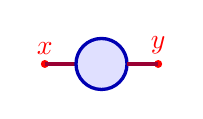
\begin{tikzpicture}[baseline=-0.45ex,scale=0.72]
  \fill[red] (-1,0) circle (2pt) node[above] {$x$};
  \fill[red] (1,0) circle (2pt) node[above] {$y$};
  \draw[purple!80!black,very thick] (-1,0)--(-0.45,0);
  \fill[blue!12,draw=blue!70!black,very thick] (0,0) circle (0.45);
  \draw[purple!80!black,very thick] (0.45,0)--(1,0);
\end{tikzpicture}
\quad=\quad
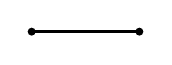
\begin{tikzpicture}[baseline=-0.45ex,scale=0.72]
  \fill (-0.95,0) circle (2pt);
  \fill (0.95,0) circle (2pt);
  \draw[very thick] (-0.95,0)--(0.95,0);
\end{tikzpicture}
\quad+\quad
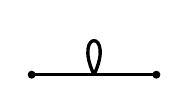
\begin{tikzpicture}[baseline=-0.45ex,scale=0.72]
  \fill (-1.1,0) circle (2pt);
  \fill (1.1,0) circle (2pt);
  \draw[very thick] (-1.1,0)--(1.1,0);
  \draw[very thick] (0,0) .. controls (-0.38,0.8) and (0.38,0.8) .. (0,0);
\end{tikzpicture}
\quad+\quad
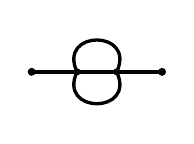
\begin{tikzpicture}[baseline=-0.45ex,scale=0.72]
  \fill (-1.15,0) circle (2pt);
  \fill (1.15,0) circle (2pt);
  \draw[very thick] (-1.15,0)--(1.15,0);
  \fill (-0.35,0) circle (1.8pt);
  \fill (0.35,0) circle (1.8pt);
  \draw[very thick] (-0.35,0) .. controls (-0.7,0.75) and (0.7,0.75) .. (0.35,0);
  \draw[very thick] (-0.35,0) .. controls (-0.7,-0.75) and (0.7,-0.75) .. (0.35,0);
\end{tikzpicture}
\quad+\cdots .
\]

\begin{definition}[Euclidean self-energy]
\label{def:euclidean-self-energy}
Define the Euclidean self-energy \(\Sigma_E(k)\) by the Dyson form
\begin{equation}
  \widetilde G_E(k)
  =
  \frac{1}{k^2+m^2-\Sigma_E(k)} .
  \label{eq:euclidean-self-energy}
\end{equation}
Equivalently,
\[
  \widetilde G_E
  =
  G_{0,E}
  +
  G_{0,E}\Sigma_E G_{0,E}
  +
  G_{0,E}\Sigma_E G_{0,E}\Sigma_E G_{0,E}
  +\cdots,
  \qquad
  G_{0,E}(k)=\frac{1}{k^2+m^2}.
\]
With this sign convention \(\Sigma_E\) is the sum of amputated connected
one-particle-irreducible two-point insertions.
\end{definition}

\[
\Sigma_E(k)
=
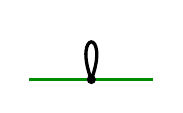
\begin{tikzpicture}[baseline=-0.45ex,scale=0.75]
  \draw[green!55!black,very thick] (-1.05,0)--(1.05,0);
  \fill (0,0) circle (2.2pt);
  \draw[very thick] (0,0) .. controls (-0.32,0.85) and (0.32,0.85) .. (0,0);
\end{tikzpicture}
\quad+\quad
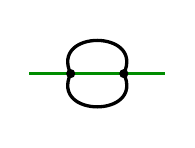
\begin{tikzpicture}[baseline=-0.45ex,scale=0.75]
  \draw[green!55!black,very thick] (-1.15,0)--(1.15,0);
  \fill (-0.45,0) circle (2.2pt);
  \fill (0.45,0) circle (2.2pt);
  \draw[very thick] (-0.45,0) .. controls (-0.8,0.75) and (0.8,0.75) .. (0.45,0);
  \draw[very thick] (-0.45,0) .. controls (-0.8,-0.75) and (0.8,-0.75) .. (0.45,0);
\end{tikzpicture}
\quad+\quad
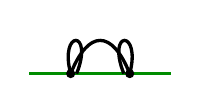
\begin{tikzpicture}[baseline=-0.45ex,scale=0.75]
  \draw[green!55!black,very thick] (-1.2,0)--(1.2,0);
  \fill (-0.5,0) circle (2.2pt);
  \fill (0.5,0) circle (2.2pt);
  \draw[very thick] (-0.5,0) .. controls (-0.7,0.75) and (-0.1,0.75) .. (-0.4,0);
  \draw[very thick] (-0.5,0) .. controls (-0.2,0.75) and (0.2,0.75) .. (0.5,0);
  \draw[very thick] (0.5,0) .. controls (0.7,0.75) and (0.1,0.75) .. (0.4,0);
\end{tikzpicture}
\quad+\cdots .
\]

\begin{proposition}[One-loop tadpole self-energy and cutoff growth]
\label{prop:one-loop-tadpole-self-energy-cutoff-growth}
The order-\(g\) tadpole is
\[
\begin{tikzpicture}[baseline=-0.45ex,scale=0.75,>=Stealth]
  \draw[green!55!black,very thick,->] (-1.1,0)--(0,0) node[midway,below] {$k$};
  \draw[green!55!black,very thick,->] (1.1,0)--(0,0) node[midway,below] {$k$};
  \fill (0,0) circle (2.2pt);
  \draw[very thick,->] (0,0) .. controls (-0.35,0.9) and (0.35,0.9) .. (0,0)
    node[midway,above] {$q$};
\end{tikzpicture}
\quad=\quad
-\frac{g}{2}
\int \frac{\dd^D q}{(2\pi)^D}\,\frac{1}{q^2+m^2}.
\]
The factor \(1/2\) is the symmetry factor of the tadpole graph. This insertion
is independent of the external momentum \(k\), because no external momentum
flows through the closed loop. In the continuum notation the loop integral is
ultraviolet divergent for \(D\ge2\). With a sharp momentum cutoff used only to
display the degree of divergence,
\[
  C_1(\Lambda,m)
  =
  \frac{1}{2}
  \int_{|q|\le\Lambda}
  \frac{\dd^D q}{(2\pi)^D}\,\frac{1}{q^2+m^2}
\]
equals
\[
  \frac{1}{2}
  \frac{\operatorname{vol}(S^{D-1})}{(2\pi)^D}
  \int_0^\Lambda \dd r\,\frac{r^{D-1}}{r^2+m^2},
  \qquad
  \operatorname{vol}(S^{D-1})
  =
  \frac{2\pi^{D/2}}{\Gamma(D/2)}.
\]
Thus
\[
  C_1(\Lambda,m)
  \sim
  \begin{cases}
    \dfrac{1}{4\pi}\log\dfrac{\Lambda}{m}, & D=2,\\[2mm]
    \dfrac{1}{2}
    \dfrac{\operatorname{vol}(S^{D-1})}{(2\pi)^D}
    \dfrac{\Lambda^{D-2}}{D-2}, & D\ge3,
  \end{cases}
\]
up to finite terms and convention-dependent cutoff terms.  The first line uses
\[
  \int_0^\Lambda
  \frac{r\,\dd r}{r^2+m^2}
  =
  \frac{1}{2}\log\frac{\Lambda^2+m^2}{m^2}
  =
  \log\frac{\Lambda}{m}+O(\Lambda^{-2})
\]
inside the radial expression. The second line uses
\(r^{D-1}(r^2+m^2)^{-1}=r^{D-3}+O(r^{D-5})\) at large \(r\).  Hence
\[
  \Sigma_E^{(1)}(k)=-g\,C_1(\Lambda,m).
\]
\end{proposition}

\begin{proof}
The coefficient \(-g/2\) is the symmetry factor computed in
Proposition~\ref{prop:automorphism-denominator-from-wick-pairings}: the two
unattached half-edges at the quartic vertex form one loop and may be
interchanged.  No external momentum enters the loop propagator, so the
amputated insertion is momentum independent and equals the displayed
regulated integral.  In spherical coordinates the cutoff integral is
\[
  \frac12
  \frac{\operatorname{vol}(S^{D-1})}{(2\pi)^D}
  \int_0^\Lambda \frac{r^{D-1}\,\dd r}{r^2+m^2}.
\]
For \(D=2\) the integral is
\(\frac12\log((\Lambda^2+m^2)/m^2)=\log(\Lambda/m)+O(\Lambda^{-2})\).
For \(D\ge3\), subtract the leading asymptotic term
\(r^{D-3}\); the remainder is lower degree at infinity, so the leading
growth is \(\Lambda^{D-2}/(D-2)\) with the displayed prefactor.  The Dyson
sign convention of Definition~\ref{def:euclidean-self-energy} then gives
\(\Sigma_E^{(1)}=-gC_1\).
\end{proof}

\begin{proposition}[Two-loop sunset insertion]
\label{prop:two-loop-sunset-insertion}
The order-\(g^2\) sunset insertion is
\[
\begin{aligned}
\begin{tikzpicture}[baseline=-0.45ex,scale=0.72,>=Stealth]
  \draw[green!55!black,very thick,->] (-1.35,0)--(-0.55,0) node[midway,below] {$k$};
  \draw[green!55!black,very thick,->] (1.35,0)--(0.55,0) node[midway,below] {$k$};
  \fill (-0.55,0) circle (2.2pt);
  \fill (0.55,0) circle (2.2pt);
  \draw[very thick,->] (-0.55,0) .. controls (-0.8,0.8) and (0.8,0.8) .. (0.55,0)
    node[midway,above] {$q_1$};
  \draw[very thick,->] (-0.55,0)--(0.55,0) node[midway,above] {$q_2$};
  \draw[very thick,->] (-0.55,0) .. controls (-0.8,-0.8) and (0.8,-0.8) .. (0.55,0)
    node[midway,below] {$k-q_1-q_2$};
\end{tikzpicture}
&=
\frac{g^2}{6}
\int \frac{\dd^D q_1\,\dd^D q_2}{(2\pi)^{2D}}
\\[-1mm]
&\quad\times
\frac{1}{
  (q_1^2+m^2)(q_2^2+m^2)
  \bigl((k-q_1-q_2)^2+m^2\bigr)} .
\end{aligned}
\]
This formula is a Euclidean integral.  Its Lorentzian boundary values are
obtained by analytic continuation with contour-deformation control; for
timelike external momentum the three-particle Landau threshold of this graph
prevents a naive independent Wick rotation of the loop energies.
\end{proposition}

\begin{proof}
The graph has two quartic vertices and three internal lines joining them.
After the two external half-edges are fixed, the remaining three internal
edges may be permuted, giving the automorphism factor \(3!\).  Thus the
coefficient is \(g^2/6\), in agreement with the Wick-pairing count in the
preceding section.  Momentum conservation at the two vertices leaves two
independent loop momenta, chosen as \(q_1,q_2\); the third internal momentum
is then \(k-q_1-q_2\).  Multiplication of the three Euclidean propagators gives
the displayed integral.  The final statement follows because the Euclidean
integral is defined on real \(D\)-momenta, while Lorentzian boundary values are
obtained by continuing external energy and deforming loop-energy contours
without crossing singularities.  At the three-particle threshold the Landau
equations allow simultaneous on-shell internal lines, so this deformation
cannot be represented as an independent rotation of each loop energy.
\end{proof}

\section{Pole Mass and Counterterm Bookkeeping}

\begin{definition}[Pole mass of an interpolating scalar field]
\label{def:pole-mass-interpolating-scalar-field}
As derived in Chapter~\ref{ch:kallen-lehmann}, the spectral representation of
the Euclidean two-point function has the form
\[
  \widetilde G_E(k)
  =
  \frac{Z}{k^2+m_*^2}
  +
  \int_{[0,\infty)}
  \frac{\dd\rho_{\mathrm c}(s)}{k^2+s},
\]
with an isolated atom at \(s=m_*^2\) when the chosen field has nonzero overlap
with a stable one-particle state. The parameter \(m_*\) is the pole mass read
from the two-point function. Equivalently, singularities of the Euclidean
function in the complex \(k^2\)-plane lie at \(k^2=-s\), and an isolated
one-particle state gives the nearest such pole when no lighter state couples to
the field. At fixed spatial momentum, the same pole appears in the complex
Euclidean energy plane at
\[
  k_D=\pm\ii\sqrt{\vec k^{\,2}+m_*^2}.
\]

The field variable \(\phi\) appearing in the regulated Lagrangian and in the
source \(J\) is the perturbative representative of an interpolating local
field.  Its renormalized two-point function is the full function
\(\widetilde G_E(k)\), with pole residue \(Z\) and continuum spectral
contributions.  The asymptotic scalar field used in scattering theory is the
free field on the isolated one-particle asymptotic Fock space with pole mass
\(m_*\) and unit residue.  Perturbation theory in this chapter locates the pole
and residue of the interpolating-field Green function; the LSZ theorem later
uses those data to project external legs onto the asymptotic one-particle
states.
\end{definition}

\begin{proposition}[One-loop pole shift and mass-coordinate prescription]
\label{prop:one-loop-pole-shift-mass-coordinate-prescription}
Using
\[
  \widetilde G_E(k)
  =
  \frac{1}{k^2+m^2-\Sigma_E(k)}
\]
and the tadpole value above, the pole position satisfies, to first order,
\[
  m_*^2=m^2+gC_1(\Lambda,m)+O(g^2)
\]
in this cutoff scheme. The parameter \(m\) is therefore a parameter of the
regulated quadratic action. Its relation to the spectral pole mass depends on
the regulator and on the prescription used to define the finite theory.
At fixed regulator, \(g\) is a bookkeeping parameter for the coefficientwise
expansion. The coefficient \(C_1(\Lambda,m)\) grows with the cutoff in
\(D\ge2\), so the product \(gC_1(\Lambda,m)\) is not uniformly small as
\(\Lambda\to\infty\). Thus the distinction between a cutoff-dependent
quadratic action coordinate and a mass defined by spectral data is
operational in the cutoff-dependent calculation.

A perturbative mass prescription introduces a renormalized parameter \(m_R\)
and a counterterm \(\delta m^2\):
\[
  m^2=m_R^2+\delta m^2,
  \qquad
  \delta m^2=\sum_{r\ge1}g^r(\delta m^2)^{(r)}.
\]
The Euclidean Lagrangian density is written as
\[
  \mathcal L_E
  =
  \frac{1}{2}(\partial\phi)^2
  +\frac{1}{2}m_R^2\phi^2
  +\frac{g}{4!}\phi^4
  +\frac{1}{2}\delta m^2\phi^2.
\]
The counterterm coefficient is part of this same regulated Lagrangian, written
in the renormalized coordinate \(m_R\).  In perturbative bookkeeping it is
treated as part of the interaction. At order \(g\), the two-valent
counterterm vertex contributes
\[
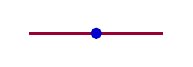
\begin{tikzpicture}[baseline=-0.45ex,scale=0.85]
  \draw[purple!80!black,very thick] (-1,0)--(1,0);
  \fill[blue!80!black] (0,0) circle (2.4pt);
\end{tikzpicture}
\qquad\longleftrightarrow\qquad
-(\delta m^2)^{(1)}g .
\]
The condition \(m_*=m_R+O(g^2)\), written at the level of squared masses,
requires
\[
  (\delta m^2)^{(1)}
  =
  -C_1(\Lambda,m_R)+\text{finite prescription term}.
\]
Different finite terms correspond to different renormalization prescriptions.
The split into \(m_R^2\) and \(\delta m^2\) is a prescription-dependent
reorganization of the regulated perturbative calculation. Its role is to make
the cancellation of cutoff-dependent local terms occur coefficient by
coefficient in the expansion in \(g\). The physical statement is made after
Green functions are expressed in terms of the chosen finite parameters, such as
the pole mass \(m_*\). In the on-shell mass prescription the finite terms are
chosen so that \(m_R=m_*\) order by order.
\end{proposition}

\begin{proof}
To first order, insert
\(\Sigma_E^{(1)}(k)=-gC_1(\Lambda,m)\) from
Proposition~\ref{prop:one-loop-tadpole-self-energy-cutoff-growth} into the
Dyson denominator:
\[
  k^2+m^2-\Sigma_E(k)
  =
  k^2+m^2+gC_1(\Lambda,m)+O(g^2).
\]
The pole in the variable \(k^2\) is therefore at
\(k^2=-m^2-gC_1(\Lambda,m)+O(g^2)\), equivalently
\(m_*^2=m^2+gC_1(\Lambda,m)+O(g^2)\).  If the quadratic coordinate of the
regulated action is rewritten as \(m_R^2+\delta m^2\), the counterterm is a
two-valent interaction vertex with the sign displayed above.  Requiring the
pole to sit at \(m_R^2\) through order \(g\) forces the order-\(g\) part of
\(\delta m^2\) to cancel \(C_1(\Lambda,m_R)\), up to the chosen finite
renormalization convention.
\end{proof}

\section{Connected Four-Point Function}

\begin{proposition}[Four-point moment-cumulant decomposition]
\label{prop:four-point-moment-cumulant-decomposition}
For four insertions, the normalized Green function decomposes into pairwise
products of two-point functions and a connected part:
\[
\begin{aligned}
  &G_{E,4}(x_1,x_2,x_3,x_4)
  \\
  &\quad =
  G_E(x_1,x_2)G_E(x_3,x_4)
  +G_E(x_1,x_3)G_E(x_2,x_4)
  +G_E(x_1,x_4)G_E(x_2,x_3)
  \\
  &\qquad
  +G_{E,4}^{\mathrm{conn}}(x_1,x_2,x_3,x_4).
\end{aligned}
\]
\end{proposition}

\begin{proof}
Apply the moment-cumulant identity to four fields.  If the theory is
\(\mathbb Z_2\)-invariant, as the regulated \(\phi^4\) theory is, all odd
cumulants vanish.  The partitions of four labels therefore contribute either
one four-label cumulant or one of the three partitions into two pairs.  The
pair cumulants are the full two-point functions \(G_E\), and the four-label
cumulant is, by definition, \(G_{E,4}^{\mathrm{conn}}\).
\end{proof}

\begin{figure}[H]
\centering
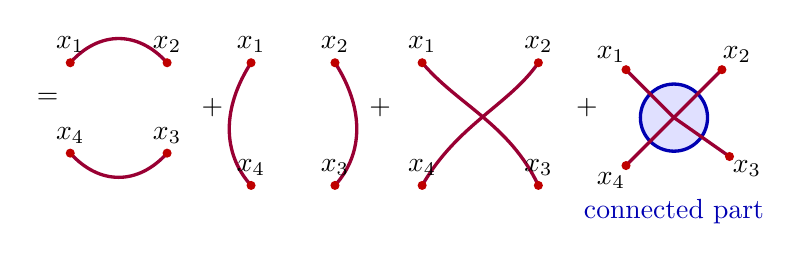
\begin{tikzpicture}[scale=0.82]
  \node at (-0.35,1.2) {$=$};
  \draw[purple!80!black,very thick] (0,1.75) .. controls (0.45,2.25) and (1.05,2.25) .. (1.5,1.75);
  \draw[purple!80!black,very thick] (0,0.35) .. controls (0.45,-0.15) and (1.05,-0.15) .. (1.5,0.35);
  \foreach \p/\lab in {(0,1.75)/x_1,(1.5,1.75)/x_2,(1.5,0.35)/x_3,(0,0.35)/x_4} {
    \fill[red!75!black] \p circle (2pt);
    \node[above] at \p {$\lab$};
  }

  \node at (2.2,1.05) {$+$};
  \draw[purple!80!black,very thick] (2.8,1.75) .. controls (2.35,1.05) and (2.35,0.35) .. (2.8,-0.15);
  \draw[purple!80!black,very thick] (4.1,1.75) .. controls (4.55,1.05) and (4.55,0.35) .. (4.1,-0.15);
  \foreach \p/\lab in {(2.8,1.75)/x_1,(4.1,1.75)/x_2,(4.1,-0.15)/x_3,(2.8,-0.15)/x_4} {
    \fill[red!75!black] \p circle (2pt);
    \node[above] at \p {$\lab$};
  }

  \node at (4.8,1.05) {$+$};
  \draw[purple!80!black,very thick] (5.45,1.75) .. controls (6.0,1.1) and (6.8,0.8) .. (7.25,-0.15);
  \draw[purple!80!black,very thick] (7.25,1.75) .. controls (6.8,1.1) and (6.0,0.8) .. (5.45,-0.15);
  \foreach \p/\lab in {(5.45,1.75)/x_1,(7.25,1.75)/x_2,(7.25,-0.15)/x_3,(5.45,-0.15)/x_4} {
    \fill[red!75!black] \p circle (2pt);
    \node[above] at \p {$\lab$};
  }

  \node at (8.0,1.05) {$+$};
  \fill[blue!12,draw=blue!70!black,very thick] (9.35,0.9) circle (0.52);
  \foreach \ang/\lab in {135/x_1,45/x_2,-35/x_3,-135/x_4} {
    \draw[purple!80!black,very thick]
      (9.35,0.9) -- ({9.35+1.05*cos(\ang)},{0.9+1.05*sin(\ang)});
    \fill[red!75!black] ({9.35+1.05*cos(\ang)},{0.9+1.05*sin(\ang)}) circle (2pt);
    \node at ({9.35+1.38*cos(\ang)},{0.9+1.38*sin(\ang)}) {$\lab$};
  }
  \node[blue!70!black] at (9.35,-0.55) {connected part};
\end{tikzpicture}
\caption{Disconnected and connected parts of the Euclidean four-point function.
The three Wick pairings are separated from
\(G_{E,4}^{\mathrm{conn}}\).}
\label{fig:four-point-wick-connected-decomposition}
\end{figure}

\begin{proposition}[Leading connected four-point Green function]
\label{prop:leading-connected-four-point-green-function}
The Fourier transform of the connected part is defined by
\[
\begin{aligned}
  G_{E,4}^{\mathrm{conn}}(x_1,\ldots,x_4)
  &=
  \int
  \prod_{i=1}^4 \frac{\dd^D k_i}{(2\pi)^D}\,
  \ee^{\ii\sum_i k_i\cdot x_i}\,
  \widetilde G_{E,4}^{\mathrm{conn}}(k_1,\ldots,k_4).
\end{aligned}
\]
To leading order,
\[
\begin{aligned}
  \widetilde G_{E,4}^{\mathrm{conn}}(k_1,\ldots,k_4)
  &=
  (2\pi)^D\delta^{(D)}(k_1+k_2+k_3+k_4)
  \\
  &\quad\times
  \left[
    -g\prod_{i=1}^4 \frac{1}{k_i^2+m^2}
    +O(g^2)
  \right].
\end{aligned}
\]
This is a connected Green function with external propagators included. Later,
after scattering states and LSZ have been constructed, the operation of
removing the external propagators will acquire its scattering interpretation.
\end{proposition}

\begin{proof}
The order-\(g\) connected four-point graph has one quartic vertex and four
labelled external endpoints.  The \(1/4!\) in the interaction is cancelled by
the \(4!\) assignments of the four labelled external fields to the four
half-edges of the vertex, so the vertex coefficient is \(-g\).  Translation
invariance supplies the momentum-conserving delta function.  Each external
field remains connected to the vertex by a Euclidean free propagator, giving
\(\prod_i(k_i^2+m^2)^{-1}\).  Since this is a Green function rather than an
amputated scattering amplitude, those external propagators are part of the
coefficient.
\end{proof}

\chapter{Lorentzian Green Functions and Analytic Continuation}
\label{ch:lorentzian-green-functions}
\ConventionsMixed


\section{Time-Ordered Boundary Values}

Let \(x^\mu=(x^0,\vec x)\in\mathbb R^{1,D-1}\) and use the mostly-plus
metric
\[
  \eta_{\mu\nu}=\operatorname{diag}(-,+,\ldots,+),
  \qquad
  k^2=\eta_{\mu\nu}k^\mu k^\nu.
\]
Write \(M=\mathbb R^{1,D-1}\).  The framework in this chapter is a scalar
Wightman field presentation in a vacuum sector: a Hilbert space \(\Hilb\), a
vacuum vector \(\vac\), a strongly continuous unitary representation of
translations with self-adjoint generators \(P^\mu\) whose joint spectrum lies
in the closed forward cone
\[
  \overline V_+=\{p\in M:p^0\ge0,\ p^2\le0\},
\]
and a scalar
operator-valued distribution \(\widehat\phi\) defined on a common invariant
dense domain.  Point-field notation denotes the kernel notation for smeared
operator-valued distributions.

For \(r\ge1\), \(\mathcal S(M^r)\) denotes the Schwartz space on \(M^r\), and
\(\mathcal S'(M^r)\) its continuous dual.  This chapter works in the tempered
distribution category:
\[
  W_r,\ G_r\in\mathcal S'(M^r).
\]
Every compactly supported smearing used to define a local field matrix element
is also a Schwartz test function, so this convention is compatible with the
local operator-valued-distribution notation.  After translation invariance is
used, analytic boundary values are paired with test functions in the relative
variables.  Thus a holomorphic function \(F\) on a tube over \(M^{r-1}\) has
boundary value \(T\in\mathcal S'(M^{r-1})\) when, for every
\(f\in\mathcal S(M^{r-1})\),
\[
  \lim_{y\to0}
  \int_{M^{r-1}}\dd^{D(r-1)}\xi\,
  F(\xi-\ii y)f(\xi)
  =
  \langle T,f\rangle ,
\]
with \(y\) approaching the real edge inside the specified tube cone.

The Wightman \(n\)-point distribution is
\[
  W_n(x_1,\ldots,x_n)
  =
  \langle \vac|
  \widehat\phi(x_1)\cdots\widehat\phi(x_n)
  |\vac\rangle
  \in \mathcal S'(M^n).
\]
For a permutation \(\pi\in S_n\), set
\[
  M_\pi^n
  =
  \{(x_1,\ldots,x_n):x_{\pi(1)}^0>\cdots>x_{\pi(n)}^0\}.
\]
A vacuum time-ordered Green function for this field is a distribution
\[
  G_n\in\mathcal S'(M^n)
\]
whose restriction to \(M_\pi^n\) is
\[
  G_n(x_1,\ldots,x_n)\big|_{M_\pi^n}
  =
  \langle \vac|
  \widehat\phi(x_{\pi(1)})\cdots
  \widehat\phi(x_{\pi(n)})
  |\vac\rangle .
\]
Equivalently, on \(M_\pi^n\) away from coincident insertion points,
\[
  G_n(x_1,\ldots,x_n)
  =
  \langle \vac|
  \widehat\phi(x_{\pi(1)})\cdots
  \widehat\phi(x_{\pi(n)})
  |\vac\rangle .
\]
Local commutativity makes the restrictions compatible across spacelike
equal-time boundaries.  A choice of \(G_n\) is therefore an extension across
partial diagonals \(x_{a_1}=\cdots=x_{a_r}\).  The possible differences
between two such extensions are local distributions supported on these
diagonals.  In perturbation theory this extension datum is fixed together
with the renormalization prescription for local products.  The compact
operator notation
\[
  G_n(x_1,\ldots,x_n)
  =
  \langle \vac|
  \operatorname T\{
    \widehat\phi(x_1)\cdots\widehat\phi(x_n)
  \}
  |\vac\rangle
\]
refers to this specified distribution.

For the free scalar field of mass \(m>0\), the two-point time-ordered Green
function has Fourier representation
\[
  \Delta_F(x;m^2)
  =
  -\ii
  \int \frac{\dd^D k}{(2\pi)^D}\,
  \frac{\ee^{\ii k\cdot x}}{k^2+m^2-\ii\epsilon},
  \qquad
  \epsilon>0.
\]
At fixed \(\vec k\), with
\[
  \omega_{\vec k}=\sqrt{\vec k^{\,2}+m^2},
\]
the poles in the complex \(k^0\)-plane are
\[
  k^0=-\omega_{\vec k}+\ii0,
  \qquad
  k^0=+\omega_{\vec k}-\ii0 .
\]
This is the Feynman boundary value of the meromorphic function of \(k^0\).

\section{Tube Analyticity From the Spectrum Condition}

The \(i\epsilon\) prescription is the two-point perturbative expression of a
more general analytic fact.  Let
\[
  W_n(x_1,\ldots,x_n)
  =
  \langle \vac|
  \widehat\phi(x_1)\cdots\widehat\phi(x_n)
  |\vac\rangle
\]
be a Wightman distribution.  By translation invariance write it in the
relative variables
\[
  \xi_j=x_j-x_{j+1},
  \qquad j=1,\ldots,n-1.
\]
Let
\[
  w_n(\xi_1,\ldots,\xi_{n-1})\in\mathcal S'(M^{n-1})
\]
be the corresponding relative-coordinate distribution.  Its Fourier transform
\(\widetilde w_n\) is defined with the convention
\[
  w_n(\xi)
  =
  \int\frac{\dd^{D(n-1)}p}{(2\pi)^{D(n-1)}}\,
  \ee^{\ii\sum_j p_j\cdot\xi_j}\widetilde w_n(p)
\]
in distribution notation.  Equivalently, for \(f\in\mathcal S(M^{n-1})\),
\[
  \langle w_n,f\rangle
  =
  \left\langle \widetilde w_n,\check f\right\rangle,
  \qquad
  \check f(p)
  =
  \int\frac{\dd^{D(n-1)}\xi}{(2\pi)^{D(n-1)}}\,
  \ee^{\ii\sum_jp_j\cdot\xi_j}f(\xi).
\]
The spectrum condition gives the support inclusion
\[
  \operatorname{supp}\widetilde w_n
  \subset
  \overline V_+^{\,n-1}.
\]
For \(\eta=(\eta_1,\ldots,\eta_{n-1})\in V_+^{n-1}\), the function
\(\exp(\sum_j p_j\cdot\eta_j)\) decreases exponentially on every closed
subcone of \(\overline V_+^{\,n-1}\) which contains the support of
\(\widetilde w_n\).  Multiplication of \(\widetilde w_n\) by this function is
therefore a well-defined tempered distribution after inserting any smooth
cutoff equal to one on a conic neighborhood of the support; the result is
independent of the cutoff.  The inverse Fourier transform is a holomorphic
function of
\begin{equation}
  z_j=\xi_j-\ii\eta_j,
  \qquad
  \eta_j\in V_+,\qquad j=1,\ldots,n-1,
  \label{eq:wightman-forward-tube}
\end{equation}
where \(V_+\) is the open future light cone.  In distribution notation this
Fourier-Laplace transform is written as
\[
  \mathcal W_n(z)
  =
  \frac{1}{(2\pi)^{D(n-1)}}
  \left\langle
    \widetilde w_n(p),
    \exp\!\left\{\ii\sum_{j=1}^{n-1}p_j\cdot z_j\right\}
  \right\rangle .
\]
Indeed, for
\(p\in\overline V_+\) and \(\eta\in V_+\), the mostly-plus inner product
satisfies
\[
  p\cdot\eta\le0,
\]
so the factor
\[
  \exp\{\ii p\cdot(\xi-\ii\eta)\}
  =
  \exp\{\ii p\cdot\xi+p\cdot\eta\}
\]
is damped rather than enlarged.
The boundary value is \(w_n\) in \(\mathcal S'(M^{n-1})\):
\[
  \lim_{\eta\to0,\ \eta_j\in V_+}
  \int_{M^{n-1}}\dd^{D(n-1)}\xi\,
  \mathcal W_n(\xi-\ii\eta)f(\xi)
  =
  \langle w_n,f\rangle,
  \qquad f\in\mathcal S(M^{n-1}).
\]

Different operator orderings give holomorphic functions in corresponding
permuted tubes.  Local commutativity identifies their boundary values on real
regions where the exchanged neighboring points are spacelike separated.

\begin{theorem}[Distributional edge-of-the-wedge statement used here]
\label{thm:distributional-edge-of-the-wedge}
Let \(U\subset\mathbb R^N\) be open, and let \(C_+\) and \(C_-\) be open
convex cones in \(\mathbb R^N\).  Suppose \(F_\pm\) are holomorphic on the
tubes \(U+\ii C_\pm\).  Assume the following polynomial boundary growth: for
every compact \(K\subset U\) and every closed cone \(C'_\pm\) whose nonzero
vectors lie in \(C_\pm\), there are constants \(A,N<\infty\) such that
\[
  |F_\pm(x+\ii y)|
  \le
  A(1+|x|)^N |y|^{-N},
  \qquad
  x\in K,\quad y\in C'_\pm,\quad 0<|y|<1.
\]
These estimates define distributional boundary values
\[
  b_\pm\in\mathcal D'(U).
\]
If \(b_+=b_-\) on a nonempty open real subset \(O\subset U\), then there is a
connected complex neighborhood \(\mathcal N\) of \(O\) and a holomorphic
function \(F\) on \(\mathcal N\) whose restrictions agree with \(F_+\) and
\(F_-\) wherever the original tubes meet \(\mathcal N\).
\end{theorem}

In the Wightman application, the polynomial growth hypothesis comes from the
tempered Fourier-Laplace construction above, and the equality of boundary
values comes from local commutativity on the spacelike real edge.  The theorem
therefore supplies the common holomorphic continuation of the permuted tube
functions across those spacelike real regions.  Time-ordered Green functions
are boundary values obtained by approaching real Lorentzian points from
imaginary time orderings compatible with the chosen operator order.  For two
points, this general construction is exactly the pole displacement
\[
  \frac1{k^2+m^2-\ii\epsilon}
\]
appearing in the Feynman propagator.

\section{Boundary-Value Dictionary}

The preceding tube statement gives a precise dictionary among Wightman,
time-ordered, and Euclidean functions.  Fix an ordering \(\pi\) and real
Lorentzian points with
\[
  x_{\pi(1)}^0>x_{\pi(2)}^0>\cdots>x_{\pi(n)}^0 .
\]
Choose positive numbers
\[
  \epsilon_1>\epsilon_2>\cdots>\epsilon_n>0
\]
and set
\[
  z_{\pi(j)}=x_{\pi(j)}-\ii\epsilon_j e_0,
  \qquad e_0=(1,\vec0).
\]
Then
\[
  z_{\pi(j)}-z_{\pi(j+1)}
  =
  x_{\pi(j)}-x_{\pi(j+1)}
  -
  \ii(\epsilon_j-\epsilon_{j+1})e_0
\]
lies in the forward tube for the \(j\)-th relative variable.  The
time-ordered boundary value on the region \(M_\pi^n\) is
\[
  G_n(x_1,\ldots,x_n)\big|_{M_\pi^n}
  =
  \lim_{\epsilon_1>\cdots>\epsilon_n\downarrow0}
  \mathcal W_{n,\pi}(z_{\pi(1)},\ldots,z_{\pi(n)}),
\]
where \(\mathcal W_{n,\pi}\) denotes the holomorphic continuation of the
Wightman ordering displayed by \(\pi\).  The limit is a distributional
boundary value: it is taken after pairing with a Schwartz test function in
the relative variables.

Euclidean Schwinger functions arise from the same holomorphic functions by
restriction to imaginary time.  For Euclidean points
\[
  x_{E,a}=(\tau_a,\vec x_a),
\]
with
\[
  \tau_{\pi(1)}>\tau_{\pi(2)}>\cdots>\tau_{\pi(n)},
\]
define
\[
  z_{\pi(j)}^0=-\ii\tau_{\pi(j)},
  \qquad
  \vec z_{\pi(j)}=\vec x_{\pi(j)} .
\]
Then
\[
\begin{aligned}
  &S_n(x_{E,1},\ldots,x_{E,n})
    \big|_{\tau_{\pi(1)}>\cdots>\tau_{\pi(n)}}  \\
  &\qquad =
  \mathcal W_{n,\pi}(z_{\pi(1)},\ldots,z_{\pi(n)}).
\end{aligned}
\]
Conversely, an OS-admissible Schwinger hierarchy reconstructs Wightman
boundary values by the positive-time quotient and analytic-continuation
theorem of Chapter~\ref{ch:volume-iv-osterwalder-schrader-reconstruction}.
Thus the boundary-value dictionary has two certified entrances: spectral
Wightman data with tube analyticity, and Euclidean data satisfying the OS
positivity, covariance, regularity, and growth hypotheses.

For \(n=2\), the dictionary gives the Feynman prescription.  If
\(x^0>0\), the ordered boundary value is obtained with the positive-energy
pole below the real \(k^0\)-axis and the negative-energy pole above it:
\[
  k^0=+\omega_{\vec k}-\ii0,
  \qquad
  k^0=-\omega_{\vec k}+\ii0.
\]
If \(x^0<0\), the contour closure selects the opposite residue in the same
single distribution \(\Delta_F\).  This two-point pole rule is the momentum
space encoding of the ordered tube boundary value above.

\section{Lorentzian Feynman Rules for Green Functions}

Consider the same scalar \(\phi^4\) interaction as in the Euclidean chapter,
with Lorentzian interaction density
\[
  \mathcal L_{\mathrm{int}}
  =
  -\frac{g}{4!}\phi^4 .
\]
The perturbative rules below compute time-ordered Green functions. They use
Lorentzian momenta on every line.

\begin{center}
\begin{tikzpicture}[scale=0.9,>=Stealth]
  \draw[purple!80!black,very thick,->] (-1.25,0)--(1.25,0)
    node[midway,above] {$k$};
  \node at (2.0,0) {$=$};
  \node at (3.35,0)
    {$\displaystyle \frac{-\ii}{k^2+m^2-\ii\epsilon}$};

  \begin{scope}[xshift=7.2cm]
    \fill[blue!80!black] (0,0) circle (2.5pt);
    \foreach \ang/\lab in {135/k_1,45/k_2,-45/k_3,-135/k_4} {
      \draw[purple!80!black,very thick,->]
        ({1.0*cos(\ang)},{1.0*sin(\ang)}) -- (0,0);
      \node at ({1.34*cos(\ang)},{1.34*sin(\ang)}) {$\lab$};
    }
    \node at (1.85,0) {$=$};
    \node[align=left,anchor=west] at (2.25,0)
      {$\displaystyle -\ii g\,(2\pi)^D
        \delta^{(D)}(k_1+k_2+k_3+k_4)$};
  \end{scope}
\end{tikzpicture}
\end{center}

This is the labelled-leg convention matching the Euclidean convention of the
previous chapter. Direct expansion of the interaction density instead assigns
\[
  -\frac{\ii g}{4!}\,(2\pi)^D
  \delta^{(D)}(k_1+k_2+k_3+k_4)
\]
to an unlabelled four-field insertion and recovers the labelled rule by
counting contractions.
In the labelled-leg convention used below, the factor \(4!\) associated with
assigning the four incident half-edges to a quartic vertex has already been
absorbed into the vertex rule \(-\ii g\).  Therefore a connected graph
\(\Gamma\) with labelled external legs carries only the residual factor
\[
  \frac{1}{|\operatorname{Aut}_{\mathrm{ext}}\Gamma|},
\]
where \(\operatorname{Aut}_{\mathrm{ext}}\Gamma\) is the automorphism group of
the graph that fixes every external label and preserves the incidence
relations.  For the tadpole graph below this residual group has order \(2\),
coming from the interchange of the two internal half-edges forming the loop;
this is why the tadpole coefficient is \(-\ii g/2\), not \(-\ii g\).

\section{Loop Rotation and the Tadpole}

The one-loop tadpole contribution to the Lorentzian two-point self-energy
insertion is
\[
\begin{tikzpicture}[baseline=-0.45ex,scale=0.75,>=Stealth]
  \draw[purple!80!black,very thick,->] (-1.1,0)--(0,0)
    node[midway,below] {$k$};
  \draw[purple!80!black,very thick,->] (1.1,0)--(0,0)
    node[midway,below] {$k$};
  \fill (0,0) circle (2.2pt);
  \draw[purple!80!black,very thick,->]
    (0,0) .. controls (-0.35,0.9) and (0.35,0.9) .. (0,0)
    node[midway,above] {$\ell$};
\end{tikzpicture}
\quad=\quad
-\frac{\ii g}{2}
\int \frac{\dd^D\ell}{(2\pi)^D}\,
\frac{-\ii}{\ell^2+m^2-\ii\epsilon}.
\]
The factor \(1/2\) is the same tadpole symmetry factor as in Euclidean
signature.  This is a combinatorial statement: the Wick contraction count
depends only on the polynomial \(\phi^4\) and on the residual graph
automorphism, while the signature-dependent factors enter separately through
the labelled Lorentzian vertex \(-\ii g\) and propagator numerator \(-\ii\).
The loop energy \(\ell^0\) is integrated along the real axis with
the Feynman pole displacement. The Euclidean integral is obtained by rotating
the contour to \(\ell^0=\ii \ell_E^D\), with the contour passing between the
two displaced poles.

\begin{center}
\begin{tikzpicture}[scale=0.95,>=Stealth]
  \draw[->,line width=0.65pt] (-3.1,0)--(3.1,0)
    node[right] {$\operatorname{Re}\ell^0$};
  \draw[->,line width=0.65pt] (0,-2.05)--(0,2.05)
    node[above] {$\operatorname{Im}\ell^0$};
  \draw[blue!70!black,very thick,->] (-2.75,0)--(2.75,0);
  \draw[green!50!black,very thick,->] (0,-1.75)--(0,1.75);
  \node[green!50!black,anchor=west,font=\small] at (0.18,1.82)
    {$\ell^0=\ii\ell_E^D$};
  \node[red!80!black] at (-1.35,0.35) {$\times$};
  \node[red!80!black] at (1.35,-0.35) {$\times$};
  \node[red!80!black,anchor=east] at (-1.52,0.92)
    {$-\omega_{\vec\ell}+\ii0$};
  \node[red!80!black,anchor=west] at (1.52,-1.02)
    {$+\omega_{\vec\ell}-\ii0$};
  \draw[orange!85!black,very thick,->]
    (0.38,1.45) .. controls (1.25,1.12) and (1.95,0.65) .. (2.45,0.08);
  \draw[orange!85!black,very thick,->]
    (-0.38,-1.45) .. controls (-1.25,-1.12) and (-1.95,-0.65) .. (-2.45,-0.08);
  \node[orange!85!black,font=\small,anchor=west] at (2.25,1.35)
    {contour rotation};
\end{tikzpicture}
\end{center}

With this orientation,
\[
\begin{gathered}
  \ell^0=\ii\ell_E^D,\qquad
  \dd\ell^0=\ii\,\dd\ell_E^D,\qquad
  \dd^D\ell=\ii\,\dd^D\ell_E,\\
  \ell^2+m^2-\ii\epsilon
  =
  -(\ell^0)^2+\vec\ell^{\,2}+m^2-\ii\epsilon
  \longrightarrow
  \ell_E^2+m^2 .
\end{gathered}
\]
Therefore the measure and propagator numerator together give
\[
  \dd^D\ell\,\frac{-\ii}{\ell^2+m^2-\ii\epsilon}
  \longrightarrow
  \ii\,\dd^D\ell_E\,\frac{-\ii}{\ell_E^2+m^2}
  =
  \dd^D\ell_E\,\frac{1}{\ell_E^2+m^2}.
\]
Including the vertex factor, this gives
\[
\begin{aligned}
  -\frac{\ii g}{2}
  \int \frac{\dd^D\ell}{(2\pi)^D}
  \frac{-\ii}{\ell^2+m^2-\ii\epsilon}
  &=
  \ii\left[
    -\frac{g}{2}
    \int \frac{\dd^D\ell_E}{(2\pi)^D}
    \frac{1}{\ell_E^2+m^2}
  \right].
\end{aligned}
\]
Thus the Lorentzian two-point insertion is \(\ii\Sigma(k)\), where
\(\Sigma(k)\) is the first-sheet analytic continuation of the Euclidean
self-energy \(\Sigma_E(k_E)\) with the sign convention of
Chapter~\ref{ch:perturbative-green-functions}.
More explicitly, in the same regulator and the same local two-point
subtraction convention, the denominator self-energy obeys
\begin{equation}
  \Sigma\bigl(k^0=\ii k_E^D,\vec k=\vec k_E\bigr)
  =
  \Sigma_E(k_E),
  \label{eq:lorentzian-euclidean-self-energy-match}
\end{equation}
where \(\Sigma_E\) is defined by
Eq.~\eqref{eq:euclidean-self-energy}.  The factor \(\ii\) displayed above
belongs to the Lorentzian two-point insertion in the Dyson series; it is not an
extra sign in the scalar function \(\Sigma\) appearing in the denominator of
\(\widetilde G(k)\).

The contour rotation just used is a special case with no external energy
flowing through the loop.  The same direct rotation is also legitimate for
loop integrals with Euclidean external momenta, where the external energies
lie on the imaginary axis and the Feynman poles can be separated continuously
from the rotating contours.  For general Lorentzian timelike external momenta,
one must instead analyze the full contour deformation in the complex loop
energy variables.  The obstruction is a pinch singularity: poles from different
propagators can trap the integration cycle so that it cannot be deformed to
the Euclidean cycle without crossing singularities.

For example, the Lorentzian continuation of the order-\(g^2\) sunset
self-energy contains the denominator product
\[
  \frac{1}{
  (q_1^2+m^2-\ii0)(q_2^2+m^2-\ii0)
  \bigl((k-q_1-q_2)^2+m^2-\ii0\bigr)} .
\]
At \(\vec k=0\), the Landau equations have a solution with all three internal
lines on shell and carrying positive energy when
\[
  (k^0)^2\ge (3m)^2 .
\]
At and above this three-particle threshold the \(q_1^0,q_2^0\) contours are
pinched.  Thus the Euclidean sunset integral defines a first-sheet analytic
function away from its Landau singularities, and the physical Lorentzian value
above threshold is the specified boundary value on the cut, not the result of
a naive independent rotation of each loop energy.  The discontinuity across
such cuts is computed by the Cutkosky rules, which are the perturbative
expression of the same spectral and unitarity structure developed in
Chapter~\ref{ch:volume-ii-analyticity-crossing-landau}.

\section{Full Two-Point Function and First Sheet}

The perturbative time-ordered two-point function is written as
\[
  G(x,y)
  =
  \int\frac{\dd^D k}{(2\pi)^D}\,
  \ee^{\ii k\cdot(x-y)}
  \widetilde G(k),
\]
where
\[
  \widetilde G(k)
  =
  \frac{-\ii}{k^2+m^2-\ii\epsilon-\Sigma(k)} .
\]
The function \(\Sigma(k)\) is initially computed for Euclidean external
momenta, where loop integrals have Euclidean denominators. Using
\[
  k^0=\ii k_E^D ,
\]
the Euclidean external energy lies on the imaginary \(k^0\)-axis. The
matching identity \eqref{eq:lorentzian-euclidean-self-energy-match} gives
\[
  \widetilde G(\ii k_E^D,\vec k_E)
  =
  -\ii\,\widetilde G_E(k_E),
\]
because \(k^2=k_E^2\) at \(k^0=\ii k_E^D\) with the mostly-plus convention.
The Lorentzian value is the boundary value obtained by analytic continuation of
\(k^0\) from this axis to the prescribed side of the real axis without crossing
the first-sheet cuts.

The spectral representation fixes the location of the first singular
thresholds. Suppose the continuum part \(d\rho_{\mathrm c}\) in the two-point
spectral measure has lowest invariant mass \(M\), meaning
\[
  M^2
  =
  \inf \operatorname{supp} d\rho_{\mathrm c}
\]
in the K\"all\'en--Lehmann variable \(s=\mu^2\).  Under the two-particle
threshold assumption stated in Chapter~\ref{ch:kallen-lehmann}, namely
\(\operatorname{supp}d\rho_{\mathrm c}\subset[4m^2,\infty)\) with the
\(\phi\phi\) continuum saturating the lower endpoint, this notation gives
\[
  M^2=4m^2,\qquad M=2m .
\]
If the first continuum channel has a different threshold, \(M\) denotes that
actual square-root threshold. At fixed spatial momentum \(\vec k\), define
\[
  E_M(\vec k)=\sqrt{\vec k^{\,2}+M^2}.
\]
The continuum denominators have singular support when
\[
  (k^0)^2=\vec k^{\,2}+s,
  \qquad s\ge M^2.
\]
Consequently the first sheet has branch cuts beginning at
\[
  k^0=+E_M(\vec k),
  \qquad
  k^0=-E_M(\vec k).
\]
The Feynman boundary value on the positive-energy cut is reached from the
upper half-plane. Thus the value of \(\Sigma(k)\) at real positive \(k^0\) is
the boundary value approached from \(\operatorname{Im}k^0>0\) on the first
sheet. The negative-energy cut is reached with the conjugate placement.

\begin{center}
\begin{tikzpicture}[scale=0.95,>=Stealth]
  \draw[->,line width=0.65pt] (-3.15,0)--(3.15,0)
    node[right] {$\operatorname{Re}k^0$};
  \draw[->,line width=0.65pt] (0,-2.05)--(0,2.05)
    node[above] {$\operatorname{Im}k^0$};
  \draw[red!80!black,very thick,decorate,
    decoration={zigzag,segment length=4pt,amplitude=1.2pt}]
    (-3.0,0)--(-1.05,0);
  \draw[red!80!black,very thick,decorate,
    decoration={zigzag,segment length=4pt,amplitude=1.2pt}]
    (1.05,0)--(3.0,0);
  \node[below] at (-1.05,-0.05) {$-E_M(\vec k)$};
  \node[below] at (1.05,-0.05) {$+E_M(\vec k)$};
  \draw[orange!85!black,very thick,->]
    (1.65,1.05) .. controls (2.2,0.82) and (2.2,0.28) .. (1.65,0.12);
  \draw[orange!85!black,very thick,->]
    (-1.65,-1.05) .. controls (-2.2,-0.82) and (-2.2,-0.28) .. (-1.65,-0.12);
  \node[orange!85!black,align=center] at (2.25,1.34)
    {positive-energy\\boundary value};
  \node[orange!85!black,align=center] at (-2.25,-1.34)
    {negative-energy\\boundary value};
\end{tikzpicture}
\end{center}

The output of the continuation is a family of Lorentzian time-ordered Green
functions with specified singularity prescriptions. The spectral poles and
cuts identify one-particle and continuum invariant masses seen by the field.
The next construction concerns asymptotic states: it asks for Hilbert-space
limits in which separated wave packets behave as freely propagating stable
particles in the far past or far future. That construction is logically
additional to the analytic continuation of Green functions.

\chapter{Haag--Ruelle Scattering Theory}
\label{ch:haag-ruelle}

\section{Scattering States as Hilbert-Space Limits}

The previous chapters constructed local fields, their spectral content, and
Lorentzian time-ordered Green functions. We now add a new kind of object:
asymptotic particle states. These are vectors in the physical Hilbert space
obtained as large-time limits of localized wave packets. Once these limits are
constructed, the scattering operator is a comparison between two Hilbert-space
identifications: one made in the far past and one made in the far future.

The construction in this chapter is for a massive stable bosonic particle. It
uses a Hilbert space \(\Hilb\), a vacuum vector \(\Omega\), local operators, the
Poincare representation, the spectrum condition, and an isolated
one-particle mass shell. These hypotheses are stated explicitly because the
large-time limit is a theorem under hypotheses, not an algebraic manipulation
of Green functions.

Let spacetime have dimension \(D\), and write \(d=D-1\). The mostly-plus
metric is
\[
  \eta_{\mu\nu}=\operatorname{diag}(-,+,\ldots,+),
  \qquad
  p^2=\eta_{\mu\nu}p^\mu p^\nu .
\]
Let \(U(a,\Lambda)\) be a strongly continuous unitary representation of the
proper orthochronous Poincare group on \(\Hilb\). Its translation subgroup is
written
\[
  U(a,\mathbf 1)=\ee^{\ii a_\mu P^\mu},
\]
where the commuting self-adjoint generators \(P^\mu\) are the
energy-momentum operators. The spectrum condition is
\[
  \operatorname{Spec}(P)\subset \overline V_+
  =
  \{p\in\mathbb R^D:p^0\ge 0,\ p^2\le 0\}.
\]
The invariant mass operator is
\[
  M^2=-P_\mu P^\mu .
\]

\begin{definition}[Massive one-particle sector]
Fix \(m>0\). A massive one-particle sector of mass \(m\) is a closed subspace
\(\Hilb_1\subset\Hilb\) such that:
\begin{enumerate}
  \item \(\Hilb_1\) reduces the Poincare representation;
  \item \(M^2=m^2\) on \(\Hilb_1\);
  \item the spectrum of \(P^\mu\) on \(\Hilb_1\) lies on
  \[
    \Sigma_m^+
    =
    \{(\omega_{\vec p},\vec p):\vec p\in\mathbb R^d\},
    \qquad
    \omega_{\vec p}=\sqrt{\vec p^{\,2}+m^2};
  \]
  \item there is an open interval around \(m^2\) in the spectrum of \(M^2\)
  whose only spectral point is \(m^2\).
\end{enumerate}
Let \(P_1\) denote the orthogonal projection from \(\Hilb\) onto \(\Hilb_1\).
\end{definition}

The last condition is the mass-gap form of stability used in this chapter. It
says that the one-particle shell is separated from the continuum. In a scalar
theory with a lightest stable particle, the picture is:
\[
\begin{tikzpicture}[baseline=-0.55ex,scale=0.94,>=Stealth]
  \draw[->,line width=0.65pt] (-0.2,0)--(7.2,0)
    node[right] {$M^2=-P^2$};
  \draw[line width=0.75pt] (0,0.12)--(0,-0.12);
  \node[below] at (0,-0.12) {vacuum};
  \draw[blue!75!black,line width=1.1pt] (2.15,0.32)--(2.15,-0.32);
  \node[blue!75!black,below] at (2.15,-0.32) {$m^2$};
  \draw[red!75!black,line width=2.2pt] (4.65,0)--(7.0,0);
  \node[red!75!black,below] at (4.65,-0.18) {$M_{\mathrm{thr}}^2$};
  \draw[decorate,decoration={brace,amplitude=5pt},gray!75]
    (2.35,0.55)--(4.45,0.55);
  \node[gray!75!black] at (3.5,0.95) {spectral gap};
\end{tikzpicture}
\]
Here \(M_{\mathrm{thr}}\) is the lowest invariant mass in the continuum channel
under discussion.

\section{Local Operators and One-Particle Wave Packets}

To state the large-time construction without domain distractions, use bounded
local operators. A bounded operator \(A\) is localized in a bounded spacetime
region \(O\) when it belongs to the local algebra \(\Obs(O)\). Locality means
that if \(O_1\) and \(O_2\) are spacelike separated, then
\[
  [A_1,A_2]=0,
  \qquad
  A_i\in\Obs(O_i).
\]
For unbounded point fields, this is the corresponding statement after
smearing and restricting to the common invariant domain on which the products
are defined.

The particle must be creatable from the vacuum by local operations. In the
present scalar setting this means that there is a local operator \(A\) such
that
\[
  P_1A\Omega\ne0 .
\]
Choose a Schwartz test function \(\chi\in\mathcal S(\mathbb R^D)\) whose
Fourier transform is supported in a small neighborhood of the positive mass
shell \(\Sigma_m^+\) and avoids the rest of the energy-momentum spectrum.
Define
\[
  B=A(\chi)
  =
  \int_{\mathbb R^D}\dd^D x\,\chi(x)\,A(x),
  \qquad
  A(x)=U(x)AU(x)^{-1}.
\]
The operator \(B\) is almost local: it is approximated in norm by local
operators in larger and larger bounded regions, with errors decreasing faster
than any inverse power of the size of the region. This property is sufficient
for the locality estimates used below.

Let \(h\in C_c^\infty(\mathbb R^d)\) be a smooth compactly supported momentum
wave packet. Define the positive-energy Klein--Gordon solution
\[
  h_t(\vec x)
  =
  \int\frac{\dd^d\vec p}{(2\pi)^d}\,
  h(\vec p)\,
  \ee^{\ii\omega_{\vec p}t-\ii\vec p\cdot\vec x}.
\]
The associated Haag--Ruelle operator is
\[
  B_t(h)
  =
  \int_{\mathbb R^d}\dd^d\vec x\,
  h_t(\vec x)\,B(t,\vec x),
  \qquad
  B(t,\vec x)=U(t,\vec x)BU(t,\vec x)^{-1}.
\]
The one-particle vector created by this family is
\[
  \psi_h:=P_1B_t(h)\Omega .
\]
It is independent of \(t\). The role of the phase in \(h_t\) is precisely to
cancel the free time evolution on the mass shell.

The velocity support of \(h\) is
\[
  V(h)
  =
  \left\{
    \frac{\vec p}{\omega_{\vec p}}:
    \vec p\in\operatorname{supp}h
  \right\}
  \subset\mathbb R^d .
\]
Stationary phase gives the spacetime localization of \(h_t\): for large
\(|t|\), the wave packet is concentrated near rays
\[
  \vec x=t\,\frac{\vec p}{\omega_{\vec p}},
  \qquad
  \vec p\in\operatorname{supp}h .
\]
Thus two wave packets with disjoint velocity supports become spacelike
separated as \(|t|\to\infty\).

\begin{center}
\begin{tikzpicture}[scale=0.94,>=Stealth]
  \draw[->,line width=0.7pt] (-3.35,-2.0)--(-3.35,2.45)
    node[above] {$x^0$};
  \draw[->,line width=0.7pt] (-3.35,-2.0)--(3.5,-2.0)
    node[right] {$\vec x$};
  \draw[gray!55,dashed] (-3.0,-1.55)--(2.75,1.85);
  \draw[gray!55,dashed] (-1.15,-1.55)--(3.15,1.45);
  \fill[blue!10,draw=blue!75!black,line width=1.0pt]
    (-1.85,-1.1) ellipse (0.58 and 0.34);
  \fill[green!12,draw=green!50!black,line width=1.0pt]
    (-0.6,-1.1) ellipse (0.58 and 0.34);
  \fill[blue!10,draw=blue!75!black,line width=1.0pt]
    (-0.35,0.65) ellipse (0.55 and 0.34);
  \fill[green!12,draw=green!50!black,line width=1.0pt]
    (1.75,0.35) ellipse (0.55 and 0.34);
  \draw[->,blue!75!black,very thick] (-1.65,-0.78)--(-0.62,0.35);
  \draw[->,green!50!black,very thick] (-0.35,-0.78)--(1.38,0.13);
  \node[blue!75!black] at (-1.15,1.03) {$V(h_1)$};
  \node[green!50!black] at (2.25,0.78) {$V(h_2)$};
  \draw[<->,purple!80!black,very thick] (0.22,0.62)--(1.18,0.48);
  \node[purple!80!black,align=center] at (0.73,1.18)
    {spacelike\\separation};
\end{tikzpicture}
\end{center}

\section{Multi-Particle Limits}

Let \(B_1,\ldots,B_n\) be almost-local operators obtained as above, and let
\(h_1,\ldots,h_n\in C_c^\infty(\mathbb R^d)\) have pairwise disjoint velocity
supports. Define the time-dependent vector
\[
  \Psi_t(h_1,\ldots,h_n)
  =
  B_{1,t}(h_1)\cdots B_{n,t}(h_n)\Omega .
\]

\begin{theorem}[Haag--Ruelle limits]
Under the assumptions stated above, the limits
\[
  \Psi^{\mathrm{out}}(h_1,\ldots,h_n)
  =
  \lim_{t\to+\infty}\Psi_t(h_1,\ldots,h_n),
\]
\[
  \Psi^{\mathrm{in}}(h_1,\ldots,h_n)
  =
  \lim_{t\to-\infty}\Psi_t(h_1,\ldots,h_n)
\]
exist in the norm topology of \(\Hilb\). The limits depend only on the
one-particle vectors
\[
  \psi_j=P_1B_{j,t}(h_j)\Omega\in\Hilb_1,
  \qquad j=1,\ldots,n,
\]
and not on the auxiliary operators \(B_j\) used to interpolate them.
\end{theorem}

The proof has two analytic inputs. First, disjoint velocity supports imply
that the effective localization regions of \(B_{j,t}(h_j)\) separate
spacelike at large \(|t|\). Locality then gives rapid decay of commutators
\[
  [B_{i,t}(h_i),B_{j,t}(h_j)]
\]
for \(i\ne j\). Second, spectral isolation of the mass shell controls the part
of \(B_{j,t}(h_j)\Omega\) orthogonal to \(\Hilb_1\). In Cook's method one
estimates \(\frac{\dd}{\dd t}\Psi_t\); the commutator terms and the
orthogonal spectral-error terms are integrable in \(t\), hence
\(\Psi_t\) is a Cauchy family at \(+\infty\) and at \(-\infty\).

For \(n=2\), the essential estimate is visible from the norm difference
\[
  \|\Psi_{t'}-\Psi_t\|^2
  =
  \langle\Psi_{t'}-\Psi_t,\Psi_{t'}-\Psi_t\rangle .
\]
The scalar products entering this expression are vacuum correlation functions
of four almost-local operators. At large positive or negative times, the two
velocity clusters are separated by spacelike distances growing linearly in
\(|t|\). The cluster property and locality reduce the large-time scalar
product to the product of the corresponding one-particle scalar products.

\section{Fock Structure}

Let
\[
  \mathcal F_s(\Hilb_1)
  =
  \bigoplus_{n=0}^\infty \Hilb_1^{\odot n}
\]
be the bosonic Fock space over \(\Hilb_1\), where
\(\Hilb_1^{\odot n}\) denotes the symmetric \(n\)-fold tensor product and
\(\Hilb_1^{\odot0}=\mathbb C\Omega_F\). The vector \(\Omega_F\) is the Fock
vacuum.

For wave packets with disjoint velocity supports, define
\[
  \Omega_{\mathrm{out}}
  (\psi_1\odot\cdots\odot\psi_n)
  =
  \Psi^{\mathrm{out}}(h_1,\ldots,h_n),
\]
\[
  \Omega_{\mathrm{in}}
  (\psi_1\odot\cdots\odot\psi_n)
  =
  \Psi^{\mathrm{in}}(h_1,\ldots,h_n),
\]
where \(\psi_j=P_1B_{j,t}(h_j)\Omega\). The theorem above makes these
definitions independent of the choice of interpolating operators. By
linearity and continuity they extend from such vectors to all of
\(\mathcal F_s(\Hilb_1)\).

The Fock inner product is reproduced by the Hilbert-space inner product of
asymptotic states:
\[
\begin{aligned}
&\left\langle
  \Psi^{\mathrm{out}}(\psi_1,\ldots,\psi_n),
  \Psi^{\mathrm{out}}(\varphi_1,\ldots,\varphi_m)
  \right\rangle_{\Hilb}
\\
&\qquad =
  \delta_{nm}
  \sum_{\sigma\in S_n}
  \prod_{j=1}^n
  \langle\psi_j,\varphi_{\sigma(j)}\rangle_{\Hilb_1},
\end{aligned}
\]
and the same formula holds for incoming states. Therefore
\[
  \Omega_{\mathrm{out}},
  \Omega_{\mathrm{in}}
  :
  \mathcal F_s(\Hilb_1)\longrightarrow \Hilb
\]
are isometries. Their ranges are the outgoing and incoming scattering
subspaces,
\[
  \Hilb_{\mathrm{out}}=\operatorname{Ran}\Omega_{\mathrm{out}},
  \qquad
  \Hilb_{\mathrm{in}}=\operatorname{Ran}\Omega_{\mathrm{in}} .
\]

The Poincare group acts on \(\mathcal F_s(\Hilb_1)\) by the free Fock
representation \(U_F\) induced from its action on \(\Hilb_1\). The
Haag--Ruelle wave operators intertwine the physical and free actions:
\[
  U(a,\Lambda)\Omega_{\mathrm{out/in}}
  =
  \Omega_{\mathrm{out/in}}U_F(a,\Lambda).
\]
This equation states that an asymptotic \(n\)-particle state transforms as
the corresponding symmetrized tensor product of one-particle Wigner states.

\begin{center}
\begin{tikzcd}[column sep=large,row sep=large]
  \mathcal F_s(\Hilb_1)
    \arrow[r,"\Omega_{\mathrm{in}}"]
    \arrow[d,"S"']
  &
  \Hilb_{\mathrm{in}}\subset\Hilb
  \\
  \mathcal F_s(\Hilb_1)
    \arrow[r,"\Omega_{\mathrm{out}}"']
  &
  \Hilb_{\mathrm{out}}\subset\Hilb
    \arrow[u,dashed,leftrightarrow]
\end{tikzcd}
\end{center}

\section{The Scattering Operator}

If
\[
  \Hilb_{\mathrm{in}}=\Hilb_{\mathrm{out}},
\]
then incoming scattering states evolve into outgoing scattering states in the
sector under consideration. The scattering operator on the asymptotic Fock
space is
\[
  S
  =
  \Omega_{\mathrm{out}}^*\Omega_{\mathrm{in}}
  :
  \mathcal F_s(\Hilb_1)\longrightarrow \mathcal F_s(\Hilb_1).
\]
When the incoming and outgoing ranges coincide, \(S\) is unitary. The matrix
element between an incoming \(n\)-particle wave packet
\(\psi_1\odot\cdots\odot\psi_n\) and an outgoing \(m\)-particle wave packet
\(\varphi_1\odot\cdots\odot\varphi_m\) is
\[
\begin{aligned}
&\left\langle
  \varphi_1\odot\cdots\odot\varphi_m,\,
  S(\psi_1\odot\cdots\odot\psi_n)
  \right\rangle_{\mathcal F_s(\Hilb_1)}
\\
&\qquad =
  \left\langle
  \Omega_{\mathrm{out}}
  (\varphi_1\odot\cdots\odot\varphi_m),\,
  \Omega_{\mathrm{in}}
  (\psi_1\odot\cdots\odot\psi_n)
  \right\rangle_{\Hilb}.
\end{aligned}
\]
This equation is the nonperturbative definition of the scattering matrix
elements in the massive sector. The right hand side is an inner product in the
physical Hilbert space; the left hand side records the same number in the
free asymptotic particle basis.

Asymptotic completeness is the stronger statement
\[
  \Hilb=\Hilb_{\mathrm{in}}=\Hilb_{\mathrm{out}}
\]
for the sector of finite-energy states under consideration. The definition of
\(S\) on the scattering sector requires equality of the incoming and outgoing
ranges. Full asymptotic completeness asserts that every physical state in the
sector is captured by such asymptotic particle data.

\section{Relation to Local Correlation Functions}

The construction above produces the \(S\)-operator from Hilbert-space limits.
It also identifies what a later reduction formula must compute. If
\(\psi_j=P_1B_{j,t}(h_j)\Omega\) and
\(\varphi_i=P_1C_{i,t}(g_i)\Omega\), then an \(m\)-out, \(n\)-in matrix
element is
\[
\begin{aligned}
&\left\langle
  \Omega_{\mathrm{out}}
  (\varphi_1\odot\cdots\odot\varphi_m),\,
  \Omega_{\mathrm{in}}
  (\psi_1\odot\cdots\odot\psi_n)
  \right\rangle_{\Hilb}
\\
&\quad =
  \lim_{T\to+\infty}
  \left\langle
  \Omega\left|
  C_{m,T}(g_m)^*\cdots C_{1,T}(g_1)^*
  B_{1,-T}(h_1)\cdots B_{n,-T}(h_n)
  \right|\Omega
  \right\rangle .
\end{aligned}
\]
For large \(T\), the outgoing packets are localized near future timelike
directions and the incoming packets near past timelike directions. Locality
permits these vacuum matrix elements to be reorganized into time-ordered
correlation functions up to terms that vanish in the scattering limit. The
next chapter turns this statement into LSZ reduction: one extracts the above
matrix elements from the one-particle poles of time-ordered Green functions.

\section{Scope of the Massive Construction}

The massive Haag--Ruelle construction gives a precise scattering theory for
stable particles whose one-particle mass shell is isolated and whose charge is
localizable by the operators used in the theory. It also provides the
reference point for more delicate asymptotic problems. Massless particles,
long-range gauge forces, infraparticle sectors, and theories with confinement
require additional asymptotic observables or modified state spaces. Those
phenomena are part of the same program of constructing large-time particle
data, but their hypotheses and limiting procedures differ from the massive
case treated here.

The logical output of this chapter is therefore fixed. A scattering operator
has been defined before any LSZ formula and before any perturbative
interpretation of Feynman graphs as scattering amplitudes. Perturbative
scattering calculations, when available, compute matrix elements of this
operator after the reduction theorem has connected the Hilbert-space limits to
Green functions.

\chapter{LSZ Reduction}
\label{ch:lsz-reduction}

\section{The Reduction Problem}

Haag--Ruelle theory defines incoming and outgoing scattering states by
large-time Hilbert-space limits. LSZ reduction is the theorem that computes
matrix elements of that already-defined scattering operator from the singular
part of time-ordered Green functions at the one-particle mass shell.

This chapter keeps the same massive scalar particle as in the Haag--Ruelle
chapter. The assumptions are:
\begin{enumerate}
  \item the particle has mass \(m>0\) and an isolated one-particle subspace
  \(\Hilb_1\);
  \item the incoming and outgoing scattering subspaces for this particle
  coincide, so the scattering operator \(S=\Omega_{\mathrm{out}}^*
  \Omega_{\mathrm{in}}\) is unitary on the asymptotic Fock space;
  \item the scalar local field \(\widehat\phi\) has nonzero one-particle
  matrix element;
  \item the time-ordered products used below have been defined as
  distributions.
\end{enumerate}

Let generalized one-particle momentum states be normalized by
\[
  \langle \vec q\,|\vec p\rangle
  =
  (2\pi)^d\,2\omega_{\vec p}\,
  \delta^d(\vec q-\vec p),
  \qquad
  \omega_{\vec p}=\sqrt{\vec p^{\,2}+m^2},
\]
where \(d=D-1\). The Lorentz-invariant mass-shell measure is
\[
  \dd\mu_m(\vec p)
  =
  \frac{\dd^d\vec p}{(2\pi)^d\,2\omega_{\vec p}} .
\]
Kernel notation such as
\[
  {}_{\mathrm{out}}\langle \vec q_1,\ldots,\vec q_m
  |\vec p_1,\ldots,\vec p_n\rangle_{\mathrm{in}}
\]
means the distributional kernel obtained after smearing all momenta with
smooth compactly supported wave packets.

\section{The One-Particle Pole}

Assume that \(\widehat\phi\) is a scalar field with
\[
  \langle\Omega|\widehat\phi(0)|\vec p\rangle
  =
  Z^{1/2},
  \qquad Z>0,
\]
for the particle species under consideration. With the normalization above,
the K\"all\'en--Lehmann measure of \(\widehat\phi\) contains the atom
\[
  \dd\rho(s)=Z\,\delta(s-m^2)\,\dd s+\dd\rho_{\mathrm{cont}}(s).
\]
Consequently the Fourier transform of the time-ordered two-point function has
the pole
\[
  \widetilde G_2(k)
  =
  \frac{-\ii Z}{k^2+m^2-\ii0}
  +
  \widetilde G_{2,\mathrm{less}}(k),
\]
where \(\widetilde G_{2,\mathrm{less}}\) has no pole at the isolated
one-particle mass shell. The number \(Z\) depends on the chosen local field.
The particle state and the \(S\)-operator are invariant data; changing the
interpolating field changes the residue factor appearing in the reduction
formula.

The operation
\[
  Z^{-1/2}\,\ii(k^2+m^2)
\]
removes an external one-particle propagator with the conventions of the
Lorentzian Green-function chapter:
\[
  Z^{-1/2}\,\ii(k^2+m^2)\,
  \frac{-\ii Z}{k^2+m^2-\ii0}
  \longrightarrow
  Z^{1/2}
\]
as a mass-shell residue. Applying one such operation to every external field
is the analytic core of LSZ reduction.

\section{Connected Truncation and External Amputation}

The pole extracted by LSZ is an external one-particle pole.  It is useful to
separate this operation from two other operations that are often compressed
in notation.  First, the connected time-ordered functions are obtained from
the generating functional by taking cumulants.  If
\[
  Z[J]=
  \left\langle\Omega\left|
  \operatorname T\exp\left(\ii\int J(x)\widehat\phi(x)\,\dd^Dx\right)
  \right|\Omega\right\rangle,
\]
then
\[
  G_N^{\rm conn}(x_1,\ldots,x_N)
  =
  \left.
  \ii^{-N}
  \frac{\delta^N \log Z[J]}
       {\delta J(x_1)\cdots\delta J(x_N)}
  \right|_{J=0}.
\]
With the sign convention for \(J\) inherited from the exponential above, this
is the cumulant part of the time-ordered distribution: it contains precisely
the vacuum-connected components.  External one-particle propagators remain
until the residue operation is applied.

Second, amputation in LSZ is residue extraction at the isolated mass shell:
\[
  \operatorname*{Res}_{k^2=-m^2}
  \widetilde G_2(k)
  =
  -\ii Z .
\]
Multiplication by \(Z^{-1/2}\ii(k^2+m^2)\) is meaningful after smearing in a
neighborhood of the mass shell and taking the boundary value.  It removes
only the external pole associated with the chosen stable particle.  Internal
propagators, threshold singularities, bound-state poles in other channels,
and contact terms remain part of the amputated connected kernel.

Thus the reduction map has three logically distinct inputs:
\[
  \begin{gathered}
  \text{time-ordered distributions}
  \longrightarrow
  \text{connected distributions}
  \\
  \longrightarrow
  \text{external one-particle residues}
  \longrightarrow
  \text{scattering matrix elements}.
  \end{gathered}
\]
The Haag--Ruelle construction supplies the last target independently of
perturbation theory; the Green functions supply a way to compute its matrix
elements when the one-particle pole hypotheses hold.

\section{Contact Terms and Interpolating Fields}

The LSZ operation depends only on the simultaneous external one-particle pole.
This fact gives two useful stability properties.

First, different definitions of time-ordered products may differ by contact
terms supported on partial diagonals, for example on \(x_i=x_j\).  In momentum
space such terms are polynomial, or more generally local, in the momenta
associated with the coincident insertions.  They have no one-particle pole in
each external variable.  After multiplication by
\[
  \prod_a (k_a^2+m^2)
\]
and taking the on-shell boundary value with separated wave packets, these
local terms do not contribute to the connected scattering kernel.  They still
matter for Ward identities, composite operators, and renormalized local
products; they are simply not external one-particle residues.

Second, the local field used in the reduction is an interpolating field.  Let
\(\widehat\phi'\) be another scalar local field with
\[
  \langle\Omega|\widehat\phi'(0)|\vec p\rangle
  =
  a\,Z^{1/2},
  \qquad a\ne0,
\]
on the same isolated one-particle subspace.  Its two-point function has
one-particle residue \(Z'=|a|^2Z\).  The LSZ factors \(Z'^{-1/2}\) remove the
changed residue, and the resulting \(S\)-matrix element is the same.  Terms in
\(\widehat\phi'\) whose vacuum-to-one-particle matrix elements vanish, such
as equation-of-motion terms of the form \((\Box-m^2)\widehat\chi\) in these
sign conventions, do not create the external particle pole and therefore drop
out of the reduction formula.  The scattering operator belongs to the
asymptotic Hilbert space; the interpolating local fields are coordinates used
to access its matrix elements.

\section{Wave-Packet Form of LSZ}

Let
\[
  q_i=(\omega_{\vec q_i},\vec q_i),
  \qquad
  p_j=(\omega_{\vec p_j},\vec p_j)
\]
be outgoing and incoming positive-energy momenta. For test wave packets
\(f_i,g_j\in C_c^\infty(\mathbb R^d)\), define the smeared scattering matrix
element
\[
\begin{aligned}
&S[f_1,\ldots,f_m;g_1,\ldots,g_n]
\\
&\quad =
  \int
  \prod_{i=1}^m \dd\mu_m(\vec q_i)\, f_i(\vec q_i)^*
  \prod_{j=1}^n \dd\mu_m(\vec p_j)\, g_j(\vec p_j)
\\
&\qquad\qquad\times
  {}_{\mathrm{out}}\langle
  \vec q_1,\ldots,\vec q_m
  |\vec p_1,\ldots,\vec p_n
  \rangle_{\mathrm{in}} .
\end{aligned}
\]
The Haag--Ruelle construction expresses this number as a large-time limit of
vacuum matrix elements of local fields. Locality moves the fields associated
with future packets to the future side of the time-ordered product and the
fields associated with past packets to the past side. After Fourier transform,
the large-time oscillatory integrals select the one-particle poles
\[
  q_i^2=-m^2,
  \qquad
  p_j^2=-m^2.
\]

In distribution form, LSZ says that the connected part of the smeared matrix
element is obtained by replacing the scattering kernel with
\[
\begin{aligned}
&\left[
  \prod_{i=1}^m Z^{-1/2}\,\ii(q_i^2+m^2)
  \prod_{j=1}^n Z^{-1/2}\,\ii(p_j^2+m^2)
  \right]
\\
&\qquad\qquad\times
  \widetilde G^{\mathrm{conn}}_{m+n}
  (q_1,\ldots,q_m,-p_1,\ldots,-p_n)
\end{aligned}
\]
and then taking the boundary value in which every \(q_i\) and \(p_j\) lies on
\(\Sigma_m^+\). Incoming physical momenta appear as \(-p_j\) in the Green
function because all momenta in
\(\widetilde G_{m+n}\) are taken to enter the time-ordered correlator.

\section{Momentum-Space Kernel}

The time-ordered \(N\)-point function is
\[
  G_N(x_1,\ldots,x_N)
  =
  \langle\Omega|
  \operatorname T\{
    \widehat\phi(x_1)\cdots\widehat\phi(x_N)
  \}
  |\Omega\rangle .
\]
Its Fourier transform is defined by
\[
  G_N(x_1,\ldots,x_N)
  =
  \int
  \prod_{a=1}^N\frac{\dd^D k_a}{(2\pi)^D}\,
  \ee^{\ii\sum_a k_a\cdot x_a}\,
  \widetilde G_N(k_1,\ldots,k_N).
\]
Translation invariance gives
\[
  \widetilde G_N(k_1,\ldots,k_N)
  =
  (2\pi)^D\delta^D(k_1+\cdots+k_N)\,
  \widetilde{\mathcal G}_N(k_1,\ldots,k_{N-1}),
\]
where \(\widetilde{\mathcal G}_N\) denotes the reduced distribution after
removing the overall momentum-conservation delta function.

For \(m\) outgoing and \(n\) incoming scalar particles, set
\[
  k_i=q_i\quad (1\le i\le m),
  \qquad
  k_{m+j}=-p_j\quad (1\le j\le n).
\]
The connected LSZ kernel is
\[
\boxed{
\begin{aligned}
&{}_{\mathrm{out}}\langle
  \vec q_1,\ldots,\vec q_m
  |\vec p_1,\ldots,\vec p_n
  \rangle_{\mathrm{in,conn}}
\\
&\quad =
  \left[
  \prod_{a=1}^{m+n} Z^{-1/2}\,\ii(k_a^2+m^2)
  \right]
  \widetilde G^{\mathrm{conn}}_{m+n}(k_1,\ldots,k_{m+n})
  \bigg|_{\mathrm{on\ shell}} .
\end{aligned}
}
\]
The vertical bar means the distributional on-shell boundary value obtained
after smearing with wave packets. The formula is a statement about
distributions; the displayed kernel is the compact notation for that
statement.

Disconnected terms are treated by the same rule, but one-particle two-point
factors reproduce the identity contribution to the scattering operator. For
two identical scalar particles,
\[
\begin{aligned}
&{}_{\mathrm{out}}\langle
  \vec q_1,\vec q_2
  |\vec p_1,\vec p_2
  \rangle_{\mathrm{in}}
\\
&\quad =
  (2\pi)^d2\omega_{\vec p_1}\delta^d(\vec q_1-\vec p_1)\,
  (2\pi)^d2\omega_{\vec p_2}\delta^d(\vec q_2-\vec p_2)
\\
&\qquad+
  (2\pi)^d2\omega_{\vec p_1}\delta^d(\vec q_2-\vec p_1)\,
  (2\pi)^d2\omega_{\vec p_2}\delta^d(\vec q_1-\vec p_2)
\\
&\qquad+
  {}_{\mathrm{out}}\langle
  \vec q_1,\vec q_2
  |\vec p_1,\vec p_2
  \rangle_{\mathrm{in,conn}} .
\end{aligned}
\]

\section{Invariant Amplitudes}

The connected kernel contains the overall conservation law
\[
  q_1+\cdots+q_m=p_1+\cdots+p_n.
\]
It is conventional to define the invariant amplitude \(\mathcal M\) by
\[
\begin{aligned}
&{}_{\mathrm{out}}\langle
  \vec q_1,\ldots,\vec q_m
  |\vec p_1,\ldots,\vec p_n
  \rangle_{\mathrm{in,conn}}
\\
&\quad =
  \ii(2\pi)^D
  \delta^D(q_1+\cdots+q_m-p_1-\cdots-p_n)\,
  \mathcal M(q_1,\ldots,q_m|p_1,\ldots,p_n).
\end{aligned}
\]
With this convention the operator identity \(S=\mathbf 1+\ii T\) gives
\[
  {}_{\mathrm{out}}\langle q|T|p\rangle
  =
  (2\pi)^D\delta^D(P_{\mathrm{out}}-P_{\mathrm{in}})\,
  \mathcal M(q|p).
\]
Here \(P_{\mathrm{out}}=\sum_i q_i\) and
\(P_{\mathrm{in}}=\sum_j p_j\).

\begin{center}
\begin{tikzpicture}[scale=0.9,>=Stealth]
  \begin{scope}
    \draw[purple!80!black,very thick,->] (-2.7,1.0)--(-1.25,0.45);
    \draw[purple!80!black,very thick,->] (-2.7,-1.0)--(-1.25,-0.45);
    \draw[purple!80!black,very thick,->] (1.25,0.45)--(2.7,1.0);
    \draw[purple!80!black,very thick,->] (1.25,-0.45)--(2.7,-1.0);
    \node[circle,draw=black,thick,minimum size=1.45cm,
      fill=blue!7] at (0,0) {\(\widetilde G_c\)};
    \node[left] at (-2.75,1.0) {$p_1$};
    \node[left] at (-2.75,-1.0) {$p_2$};
    \node[right] at (2.75,1.0) {$q_1$};
    \node[right] at (2.75,-1.0) {$q_2$};
  \end{scope}
  \node at (3.45,0) {$\xrightarrow{\;\prod Z^{-1/2}\ii(k^2+m^2)\;}$};
  \begin{scope}[xshift=7.0cm]
    \draw[purple!80!black,very thick,->] (-1.65,0.8)--(-0.55,0.28);
    \draw[purple!80!black,very thick,->] (-1.65,-0.8)--(-0.55,-0.28);
    \draw[purple!80!black,very thick,->] (0.55,0.28)--(1.65,0.8);
    \draw[purple!80!black,very thick,->] (0.55,-0.28)--(1.65,-0.8);
    \node[circle,draw=black,thick,minimum size=1.15cm,
      fill=green!8] at (0,0) {\(\mathcal M\)};
  \end{scope}
\end{tikzpicture}
\end{center}

The diagram displays the operation. The left object is the connected
time-ordered Green function with its external one-particle poles. The right
object is the on-shell invariant amplitude obtained after the pole residues
have been extracted.

\section{Perturbative Evaluation After Reduction}

Perturbation theory supplies an expansion of the time-ordered Green function.
LSZ then turns that expansion into an expansion of matrix elements of the
scattering operator. This is the point where Feynman graphs acquire their
scattering-amplitude interpretation.

For the scalar interaction
\[
  \mathcal L_{\mathrm{int}}=-\frac{g}{4!}\phi^4,
\]
the leading connected four-point Green function is
\[
\begin{aligned}
&\widetilde G^{\mathrm{conn}}_4
  (q_1,q_2,-p_1,-p_2)
\\
&\quad =
  (2\pi)^D\delta^D(q_1+q_2-p_1-p_2)
  (-\ii g)
  \prod_{a=1}^4
  \frac{-\ii}{k_a^2+m^2-\ii0}
  +O(g^2),
\end{aligned}
\]
with
\[
  k_1=q_1,\quad k_2=q_2,\quad k_3=-p_1,\quad k_4=-p_2,
  \qquad
  Z=1+O(g^2).
\]
Applying LSZ gives
\[
  {}_{\mathrm{out}}\langle
  \vec q_1,\vec q_2
  |\vec p_1,\vec p_2
  \rangle_{\mathrm{in,conn}}
  =
  (2\pi)^D\delta^D(q_1+q_2-p_1-p_2)
  \left[-\ii g+O(g^2)\right].
\]
Therefore
\[
  \mathcal M(q_1,q_2|p_1,p_2)
  =
  -g+O(g^2)
\]
with the amplitude convention above. Higher orders are obtained from the
same Green-function expansion together with the external residue factors
\(Z^{-1/2}\).

\section{Scope of the Formula}

The LSZ theorem in this chapter applies to stable massive particles
represented by isolated one-particle poles in local-field Green functions. It
is a statement about boundary values of distributions after wave-packet
smearing. Its hypotheses include the existence of the asymptotic states
constructed in Haag--Ruelle theory and the existence of the relevant
time-ordered products.

Massless gauge theories, infraparticle sectors, confined degrees of freedom,
unstable resonances, and conformal theories require different asymptotic
objects or different observables. The common principle remains the same:
first construct the asymptotic Hilbert-space or detector data, then relate
that data to correlation functions in the regime where a reduction theorem is
available.

\chapter{Cross Sections, Phase Space, and Unitarity}
\label{ch:cross-sections-unitarity}

\section{Transition Probabilities}

Let \(\mathcal H_{\rm as}\) be the asymptotic Hilbert space in a sector where
the incoming and outgoing Haag--Ruelle ranges coincide.  The scattering
operator
\[
  S:\mathcal H_{\rm as}\to\mathcal H_{\rm as}
\]
is then unitary.  Write
\[
  S=\mathbf 1+\ii T .
\]
For a normalized incoming vector \(\Psi_{\rm in}\in\mathcal H_{\rm as}\) and
an outgoing class of states \(\mathcal D\), let
\(\Pi_{\mathcal D}^{\rm out}\) be the orthogonal projection onto the closed
subspace spanned by \(\mathcal D\).  The transition probability into
\(\mathcal D\) is
\[
  P_{\Psi\to\mathcal D}
  =
  \left\|
    \Pi_{\mathcal D}^{\rm out}S\Psi_{\rm in}
  \right\|^2 .
\]
This is the primary definition.  Sharp-momentum formulas are distributional
kernels obtained from this expression after smearing with wave packets and
then taking a narrow-packet limit.

For positive-energy momenta in the mostly-plus metric,
\[
  p_i=(E_i,\vec p_i),
  \qquad
  q_a=(E_a,\vec q_a),
\]
with
\[
  p_i^2=-m_i^2,\qquad q_a^2=-M_a^2,
\]
set
\[
  P_{\rm in}=\sum_i p_i,
  \qquad
  P_{\rm out}=\sum_a q_a .
\]
The invariant amplitude convention inherited from LSZ is
\[
  \langle q_1,\ldots,q_m|T|p_1,\ldots,p_n\rangle
  =
  (2\pi)^D\delta^D(P_{\rm out}-P_{\rm in})
  \mathcal M(q_1,\ldots,q_m|p_1,\ldots,p_n).
\]
The bra and ket are generalized basis vectors in \(\mathcal H_{\rm as}\).
Equivalently, the same distribution is obtained from the connected part of
the Haag--Ruelle kernel
\[
  {}_{\rm out}\langle q_1,\ldots,q_m|p_1,\ldots,p_n\rangle_{\rm in}
\]
after subtracting the identity contribution.  The connected contribution to
\(S\) is therefore
\[
  \ii(2\pi)^D\delta^D(P_{\rm out}-P_{\rm in})\mathcal M .
\]

\section{Wave-Packet Origin of Cross Sections}

Cross sections are transition probabilities per incoming transverse flux.
Let \(\psi_1,\psi_2\in\Hilb_1\) be normalized incoming one-particle packets
with narrow momentum supports and distinct group velocities.  In the
center-of-mass frame let \(\vec p_*\) be the central momentum of the first
packet, and let
\[
  \mathbb R^{D-2}_\perp
  =
  \{b\in\mathbb R^{D-1}: b\cdot \vec p_*=0\}
\]
be the transverse impact-parameter plane.  If \(\tau_b\) denotes the spatial
translation acting on the one-particle Hilbert space, define
\[
  \Psi_b=\psi_1\odot \tau_b\psi_2 .
\]
Here \(\odot\) denotes the two-particle product in the asymptotic Fock space,
with the species labels and Bose or Fermi statistics appropriate to the
sector under consideration.  For an outgoing channel \(\mathcal D\) whose
projection removes the identity no-scattering component, the wave-packet
cross section is
\[
  \sigma_{\psi_1,\psi_2}(\mathcal D)
  =
  \int_{\mathbb R^{D-2}_\perp}\dd^{D-2}b\,
  \left\|
    \Pi_{\mathcal D}^{\rm out}S\Psi_b
  \right\|^2 .
\]
The dimension is length to the power \(D-2\), the dimension of transverse
area in \(D\) spacetime dimensions.

The plane-wave formula is the narrow-packet density of this Hilbert-space
quantity.  The Fourier transform in \(b\) enforces transverse momentum
conservation.  The long-time Haag--Ruelle localization enforces energy and
longitudinal momentum conservation in the scattering limit.  Together these
produce the single overall distribution
\[
  (2\pi)^D\delta^D(P_{\rm out}-P_{\rm in})
\]
appearing in the invariant amplitude convention.  The incoming current
through the transverse impact-parameter plane is the invariant relative speed
multiplied by the one-particle normalizations.  Thus the denominator in the
sharp-momentum two-particle formula is the invariant flux
\[
  \mathcal F(p_1,p_2)=4E_1E_2v_{\rm rel}.
\]
The next section expresses the same factor in covariant form.

\section{Invariant Phase Space and Flux}

For one on-shell final particle of mass \(M\), the Lorentz-invariant
positive-energy measure is
\[
  \dd\mu_M(q)
  =
  \frac{\dd^Dq}{(2\pi)^{D-1}}\,
  \theta(q^0)\delta(q^2+M^2)
  =
  \frac{\dd^{D-1}\vec q}{(2\pi)^{D-1}2E_{\vec q}},
\]
where
\[
  E_{\vec q}=\sqrt{\vec q^{\,2}+M^2}.
\]
For \(m\) final particles with total incoming momentum \(P\), define the
\(m\)-body phase-space measure
\[
  \dd\Phi_m(P;q_1,\ldots,q_m)
  =
  (2\pi)^D\delta^D\!\left(P-\sum_{a=1}^m q_a\right)
  \prod_{a=1}^m\dd\mu_{M_a}(q_a).
\]
If some final particles are identical, the phase-space integral over labeled
momenta is divided by the factorial of the number of identical particles of
each species.

For a two-particle initial state, the invariant flux factor is
\[
  \mathcal F(p_1,p_2)
  =
  4\sqrt{(p_1\cdot p_2)^2-m_1^2m_2^2}.
\]
Equivalently,
\[
  \mathcal F=4E_1E_2v_{\rm rel},
  \qquad
  v_{\rm rel}
  =
  \frac{\sqrt{(p_1\cdot p_2)^2-m_1^2m_2^2}}{E_1E_2}.
\]
In the center-of-mass frame,
\[
  p_1=(E_1,\vec p_*),
  \qquad
  p_2=(E_2,-\vec p_*),
\]
so
\[
  \mathcal F=4(E_1+E_2)|\vec p_*|.
\]

The differential cross section for
\[
  p_1+p_2\longrightarrow q_1+\cdots+q_m
\]
is
\[
  \dd\sigma
  =
  \frac{1}{\mathcal F(p_1,p_2)}
  \left|\mathcal M(q_1,\ldots,q_m|p_1,p_2)\right|^2
  \dd\Phi_m(P_{\rm in};q_1,\ldots,q_m).
\]
All factors in this expression have now been fixed: the asymptotic state
normalization, the amplitude convention, the final-state measure, and the
incoming flux.

\begin{center}
\begin{tikzpicture}[scale=0.86,>=Stealth]
  \draw[blue!75!black,very thick,->] (-4.4,-0.9)--(-1.35,-0.22);
  \draw[green!50!black,very thick,->] (-4.4,0.9)--(-1.35,0.22);
  \draw[purple!80!black,thick,fill=purple!7]
    (-1.15,0) ellipse (0.35 and 1.05);
  \draw[red!75!black,very thick,->] (-0.72,0.28)--(2.05,1.1);
  \draw[red!75!black,very thick,->] (-0.72,0)--(2.15,0.0);
  \draw[red!75!black,very thick,->] (-0.72,-0.28)--(2.0,-1.1);
  \node[blue!75!black] at (-3.45,-1.2) {$p_1,\ \vec v_1$};
  \node[green!50!black] at (-3.45,1.2) {$p_2,\ \vec v_2$};
  \node[purple!80!black,align=center] at (-1.15,-1.55)
    {effective\\area \(\sigma\)};
  \node[red!75!black] at (2.55,1.1) {$q_1$};
  \node[red!75!black] at (2.55,0.0) {$q_2$};
  \node[red!75!black] at (2.55,-1.1) {$q_m$};
  \node[align=center] at (4.1,0)
    {final\\channel};
  \node[align=center] at (-4.15,0)
    {\(\mathcal F=4E_1E_2v_{\rm rel}\)};
\end{tikzpicture}
\end{center}

\section{Two-Body Final States in Four Dimensions}

Set \(D=4\).  For a two-body final state, define
\[
  s=-(p_1+p_2)^2=P_{\rm in}^0{}^2-\vec P_{\rm in}^{\,2}.
\]
In the center-of-mass frame,
\[
  P_{\rm in}=(\sqrt s,\vec0).
\]
The Kallen polynomial is
\[
  \lambda_K(s,a,b)=s^2+a^2+b^2-2sa-2sb-2ab .
\]
For incoming masses \(m_1,m_2\) and final masses \(M_1,M_2\),
\[
  |\vec p_*|
  =
  \frac{\sqrt{\lambda_K(s,m_1^2,m_2^2)}}{2\sqrt s},
  \qquad
  |\vec q_*|
  =
  \frac{\sqrt{\lambda_K(s,M_1^2,M_2^2)}}{2\sqrt s}.
\]
Performing the two-body phase-space integral over the energy-conserving
delta function gives
\[
  \dd\Phi_2
  =
  \frac{1}{16\pi^2}
  \frac{|\vec q_*|}{\sqrt s}\,\dd\Omega ,
\]
where \(\dd\Omega\) is the solid-angle measure of one final momentum in the
center-of-mass frame.  The flux is
\[
  \mathcal F=4\sqrt s\,|\vec p_*|.
\]
Therefore
\[
  \frac{\dd\sigma}{\dd\Omega}
  =
  \frac{1}{64\pi^2s}
  \frac{|\vec q_*|}{|\vec p_*|}
  |\mathcal M(s,\Omega)|^2 .
\]
For identical final particles, the right hand side is divided by \(2\) when
the integral is taken over the full labeled solid angle.

For elastic scattering of identical scalar particles of mass \(m\),
\[
  |\vec q_*|=|\vec p_*|,
  \qquad
  \sqrt s=E_{\rm cm}.
\]
If the tree-level \(\phi^4\) invariant amplitude is
\[
  \mathcal M=-g+O(g^2),
\]
then
\[
  \sigma_{2\to2}
  =
  \frac{g^2}{32\pi s}+O(g^3)
\]
for identical final particles.

\section{Unitarity and the Optical Theorem}

The operator identity
\[
  S^\dagger S=\mathbf 1,\qquad S=\mathbf 1+\ii T,
\]
is equivalent to
\[
  -\ii(T-T^\dagger)=T^\dagger T .
\]
Let \(i\) and \(f\) denote incoming and outgoing asymptotic momentum labels,
including all discrete quantum numbers.  Insert a complete set of outgoing
asymptotic states between \(T^\dagger\) and \(T\).  After removing the common
overall momentum-conservation delta function, the sharp-kernel form is
\[
  -\ii\left[
  \mathcal M(f|i)-\mathcal M(i|f)^*
  \right]
  =
  \sum_X
  \int\dd\Phi_X\,
  \mathcal M(X|f)^*\mathcal M(X|i),
\]
where \(X\) runs over all allowed multiparticle channels and
\(\dd\Phi_X\) includes the corresponding phase-space measure and symmetry
factors.

For \(f=i\), this becomes the optical theorem
\[
  2\,\operatorname{Im}\mathcal M(i|i)
  =
  \sum_X
  \int\dd\Phi_X\,|\mathcal M(X|i)|^2 .
\]
For two incoming particles,
\[
  \sigma_{\rm tot}
  =
  \frac{2\,\operatorname{Im}\mathcal M(i|i)}
  {\mathcal F(p_1,p_2)} .
\]
The amplitude on the left is the forward amplitude: the outgoing labels are
the same as the incoming labels.

\section{Partial Waves in Four Dimensions}

For scalar \(2\to2\) scattering in the center-of-mass frame, rotational
invariance makes the amplitude a function of \(s\) and
\[
  x=\cos\theta=\widehat p_*\cdot\widehat q_* .
\]
For distinguishable particles use the partial-wave expansion
\[
  \mathcal M(s,x)
  =
  16\pi
  \sum_{\ell=0}^{\infty}
  (2\ell+1)a_\ell(s)P_\ell(x),
\]
where \(P_\ell\) is the Legendre polynomial.  The inverse formula is
\[
  a_\ell(s)
  =
  \frac{1}{32\pi}
  \int_{-1}^1\dd x\,
  P_\ell(x)\mathcal M(s,x).
\]
For equal incoming masses in the elastic region, define
\[
  \rho(s)=\frac{2|\vec p_*|}{\sqrt s}.
\]
The partial-wave \(S\)-matrix eigenvalue is
\[
  S_\ell(s)=1+2\ii\rho(s)a_\ell(s).
\]
Elastic unitarity is
\[
  |S_\ell(s)|=1.
\]
Equivalently, there is a real phase shift \(\delta_\ell(s)\) such that
\[
  S_\ell(s)=\ee^{2\ii\delta_\ell(s)}
\]
and
\[
  a_\ell(s)
  =
  \frac{\ee^{2\ii\delta_\ell(s)}-1}{2\ii\rho(s)}
  =
  \frac{\ee^{\ii\delta_\ell(s)}\sin\delta_\ell(s)}{\rho(s)} .
\]
The same condition can be written
\[
  \operatorname{Im}a_\ell(s)=\rho(s)|a_\ell(s)|^2 .
\]
With inelastic channels open,
\[
  |S_\ell(s)|\le1,
\]
with equality precisely in a purely elastic partial wave.

For distinguishable scalar particles, the elastic total cross section is
\[
  \sigma_{\rm el}
  =
  \frac{\pi}{|\vec p_*|^2}
  \sum_{\ell=0}^\infty
  (2\ell+1)|S_\ell(s)-1|^2
  =
  \frac{4\pi}{|\vec p_*|^2}
  \sum_{\ell=0}^\infty
  (2\ell+1)\sin^2\delta_\ell(s).
\]

For identical scalar bosons, the physical two-particle amplitude on unordered
states is Bose symmetric.  With the convention
\[
  \mathcal M_{\rm id}(s,x)
  =
  32\pi
  \sum_{\substack{\ell=0\\ \ell\ {\rm even}}}^{\infty}
  (2\ell+1)a_\ell(s)P_\ell(x),
\]
and the full-solid-angle final-state factor \(1/2\), the elastic cross
section is
\[
  \sigma_{\rm el}^{\rm id}
  =
  \frac{2\pi}{|\vec p_*|^2}
  \sum_{\substack{\ell=0\\ \ell\ {\rm even}}}^{\infty}
  (2\ell+1)|S_\ell(s)-1|^2 .
\]
This is the convention used later for identical-particle high-energy bounds.

\section{Partial-Wave Unitarity Geometry}

Define
\[
  b_\ell(s)=\rho(s)a_\ell(s),
  \qquad
  S_\ell(s)=1+2\ii b_\ell(s).
\]
In an elastic partial wave, \(|S_\ell|=1\).  Writing
\[
  b_\ell=x_\ell+\ii y_\ell,
\]
this condition becomes
\[
  x_\ell^2+\left(y_\ell-\frac12\right)^2=\frac14 .
\]
Thus the elastic amplitude lies on the circle of radius \(1/2\) centered at
\(\ii/2\) in the complex \(b_\ell\)-plane.  Equivalently,
\[
  y_\ell=|b_\ell|^2 .
\]
The phase-shift form
\[
  b_\ell=\ee^{\ii\delta_\ell}\sin\delta_\ell
\]
parametrizes this circle.

When inelastic channels are open, the elastic partial wave is a matrix
element of a unitary matrix on a larger channel space.  It is convenient to
write
\[
  S_\ell=\eta_\ell\ee^{2\ii\delta_\ell},
  \qquad
  0\le\eta_\ell\le1 .
\]
Then \(b_\ell=(S_\ell-1)/(2\ii)\) lies inside the same circle:
\[
  x_\ell^2+\left(y_\ell-\frac12\right)^2\le\frac14,
  \qquad
  y_\ell\ge |b_\ell|^2 .
\]
The difference
\[
  y_\ell-|b_\ell|^2
  =
  \frac{1-\eta_\ell^2}{4}
\]
is the contribution of inelastic final states in that angular-momentum
channel.  This is the partial-wave form of the optical theorem.

\section{Thresholds, Poles, and Resonances}

The same variables organize the analytic structure of scattering.  A
threshold is the value of \(s\) at which a new on-shell intermediate channel
becomes kinematically available.  Across such a threshold, unitarity gives
the discontinuity of amplitudes in terms of phase-space integrals over lower
amplitudes.

A stable bound state in a two-particle channel appears as a pole of the
partial-wave amplitude on the physical sheet below threshold.  A resonance is
represented by a pole reached after analytic continuation through a unitarity
cut.  The precise sheet and residue statements require the analytic
continuation machinery developed later, but the organizing data are already
present here: the \(S\)-operator, phase space, unitarity, and partial waves.

\chapter{Massive Particles and Spin}
\label{ch:massive-particles-spin}

\section{Massive One-Particle Representations}

This chapter works in \(D=4\). Let \(\Hilb_1\) be an irreducible massive
one-particle subspace of mass \(m>0\). The positive-energy mass shell is
\[
  \Sigma_m^+
  =
  \{p=(p^0,\vec p):p^0=\omega_{\vec p},\ p^2=-m^2\},
  \qquad
  \omega_{\vec p}=\sqrt{\vec p^{\,2}+m^2}.
\]
Generalized momentum states are normalized by
\[
  \langle \vec q,\tau|\vec p,\sigma\rangle
  =
  (2\pi)^3\,2\omega_{\vec p}\,
  \delta^3(\vec q-\vec p)\,\delta_{\tau\sigma}.
\]
The labels \(\sigma,\tau\) span a finite-dimensional internal vector space
which is fixed by Lorentz symmetry.

Choose the reference momentum
\[
  p_R=(m,\vec0).
\]
For every \(p\in\Sigma_m^+\), choose a standard Lorentz transformation
\[
  L(p)\in SO^+(1,3),
  \qquad
  L(p)p_R=p.
\]
The stabilizer of \(p_R\) is the rotation group \(SO(3)\). Its double cover
\[
  \operatorname{Spin}(3)\simeq SU(2)
\]
acts on quantum states because Hilbert-space symmetries act on rays and may
therefore be projective before lifting to the simply connected cover.
In state-space formulas below the Lorentz transformations are understood as
elements of the universal cover when they are inserted into spin
representations; the same letters denote their projections to
\(SO^+(1,3)\) when they act on four-vectors.

For a Lorentz transformation \(\Lambda\), define the Wigner rotation
\[
  W(\Lambda,p)
  =
  L(\Lambda p)^{-1}\Lambda L(p).
\]
It obeys
\[
  W(\Lambda,p)p_R=p_R,
\]
and is therefore an element of the massive little group. If the particle has
spin \(j\), with
\[
  j=0,\frac12,1,\frac32,\ldots,
\]
let \(D^{(j)}\) be the corresponding irreducible unitary representation of
\(SU(2)\) on a vector space \(V_j\) of dimension \(2j+1\). The one-particle
states transform as
\[
  U(\Lambda)|\vec p,\sigma\rangle
  =
  \sum_{\tau=-j}^{j}
  D^{(j)}_{\tau\sigma}\!\left(W(\Lambda,p)\right)
  |\Lambda\vec p,\tau\rangle ,
\]
where \(\sigma,\tau=-j,-j+1,\ldots,j\). The covariant normalization above
absorbs the Jacobian of the mass-shell measure, so no additional
\(\sqrt{(\Lambda p)^0/p^0}\) factor appears.

\begin{center}
\begin{tikzpicture}[scale=0.95,>=Stealth]
  \draw[blue!70!black,thick] (-3.0,0) ellipse (1.55 and 1.05);
  \node[blue!70!black] at (-3.0,1.35) {$SO(3)$};
  \fill (-3.75,0) circle (2pt) node[left] {\(1\)};
  \fill (-2.25,0) circle (2pt) node[right] {\(2\pi\)};
  \draw[purple!80!black,very thick,->]
    (-3.65,-0.14).. controls (-3.35,-0.72) and (-2.65,-0.72) .. (-2.35,-0.14);
  \node[purple!80!black,fill=white,inner sep=1.5pt] at (-3.0,-1.18)
    {closed loop};

  \draw[->,gray!70,very thick] (-0.85,0)--(0.85,0)
    node[midway,above] {lift};

  \draw[green!50!black,thick] (3.0,0) ellipse (1.75 and 1.12);
  \node[green!50!black] at (3.0,1.38) {$SU(2)$};
  \fill (2.1,0) circle (2pt) node[left] {\(1\)};
  \fill (3.9,0) circle (2pt) node[right] {\(-1\)};
  \draw[red!75!black,very thick,->]
    (2.25,-0.15).. controls (2.7,-0.72) and (3.3,-0.72) .. (3.75,-0.15);
  \node[red!75!black,fill=white,inner sep=1.5pt] at (3.0,-0.94) {\(2\pi\)};
  \draw[orange!80!black,very thick,->]
    (3.75,0.15).. controls (3.3,0.72) and (2.7,0.72) .. (2.25,0.15);
  \node[orange!80!black,fill=white,inner sep=1.5pt] at (3.0,0.94) {\(4\pi\)};
\end{tikzpicture}
\end{center}

A \(2\pi\) rotation acts on \(V_j\) by
\[
  (-1)^{2j}.
\]
Integer and half-integer spins are therefore distinct representations of the
same massive little-group construction.

\section{Spin Frames on the Mass Shell}

The choice of standard transformations \(L(p)\) is a choice of spin frame over
the mass shell. To make this statement precise, let
\[
  d\mu_m(p)=\frac{d^3p}{(2\pi)^3\,2\omega_{\vec p}}
\]
be the invariant measure on \(\Sigma_m^+\). After choosing \(L(p)\), the
one-particle Hilbert space is represented as
\[
  \Hilb_1\simeq L^2(\Sigma_m^+,d\mu_m;V_j).
\]
The generalized basis associated to this frame is the distributional map
\[
  F_L(p):V_j\longrightarrow \Hilb_1,
  \qquad
  F_L(p)e_\sigma=|\vec p,\sigma\rangle ,
\]
where \(\{e_\sigma\}_{\sigma=-j}^j\) is an orthonormal basis of \(V_j\).
The Lorentz action is
\[
  U(\Lambda)F_L(p)
  =
  F_L(\Lambda p)D^{(j)}(W(\Lambda,p)).
\]
This formula is a representation of the Lorentz group because the Wigner
rotation obeys the cocycle identity
\[
  W(\Lambda_2\Lambda_1,p)
  =
  W(\Lambda_2,\Lambda_1 p)W(\Lambda_1,p).
\]
Indeed,
\[
\begin{aligned}
  W(\Lambda_2\Lambda_1,p)
  &=
  L(\Lambda_2\Lambda_1p)^{-1}\Lambda_2\Lambda_1L(p)       \\
  &=
  L(\Lambda_2\Lambda_1p)^{-1}\Lambda_2L(\Lambda_1p)\,
  L(\Lambda_1p)^{-1}\Lambda_1L(p).
\end{aligned}
\]

If \(Q:\Sigma_m^+\to SU(2)\) is a smooth little-group-valued function, then
\[
  L'(p)=L(p)Q(p)
\]
is another choice of standard transformations. The corresponding Wigner
rotation is
\[
  W'(\Lambda,p)
  =
  Q(\Lambda p)^{-1}W(\Lambda,p)Q(p).
\]
The associated generalized basis is
\[
  F_{L'}(p)=F_L(p)D^{(j)}(Q(p)).
\]
Thus a wavefunction written as a column \(\psi_L(p)\in V_j\) in the \(L\)
frame is written in the \(L'\) frame as
\[
  \psi_{L'}(p)=D^{(j)}(Q(p))^{-1}\psi_L(p).
\]
The inner product
\[
  \langle \psi,\chi\rangle
  =
  \int_{\Sigma_m^+} d\mu_m(p)\,
  \psi_L(p)^\dagger\chi_L(p)
\]
is independent of the spin frame because \(D^{(j)}(Q(p))\) is unitary. In this
language, a scattering amplitude with external massive spin states is a
multilinear pairing of spin-frame components and dual spin-frame components
whose value is invariant under the simultaneous transformations above.

\section{Covariant Fields as Intertwiners}

Let \(\widehat\Phi_A(x)\) be a local field whose index \(A\) transforms in a
finite-dimensional representation \(R\) of the double cover
\(\operatorname{Spin}^+(1,3)\simeq SL(2,\mathbb C)\):
\[
  U(\Lambda)\widehat\Phi_A(x)U(\Lambda)^{-1}
  =
  R_A{}^B(\Lambda)\widehat\Phi_B(\Lambda x).
\]
The vacuum-to-particle matrix element is
\[
  \langle\Omega|\widehat\Phi_A(0)|\vec p,\sigma\rangle
  =
  u_A{}^\sigma(p).
\]
Translation covariance gives the spacetime dependence
\[
  \langle\Omega|\widehat\Phi_A(x)|\vec p,\sigma\rangle
  =
  \ee^{\ii p\cdot x}u_A{}^\sigma(p).
\]
Lorentz covariance and the Wigner transformation law imply
\[
  \sum_{\tau=-j}^j
  u_A{}^\tau(\Lambda p)
  D^{(j)}_{\tau\sigma}(W(\Lambda,p))
  =
  R_A{}^B(\Lambda^{-1})u_B{}^\sigma(p).
\]
This is the equivariance condition that connects the covariant field index
\(A\) to the spin-frame index \(\sigma\).

At the reference momentum \(p_R\), the matrix
\[
  u_A{}^\sigma(p_R):V_j\longrightarrow R|_{SU(2)}
\]
is an intertwiner of \(SU(2)\) representations:
\[
  R(W)_A{}^B u_B{}^\sigma(p_R)
  =
  \sum_{\tau=-j}^j
  u_A{}^\tau(p_R)D^{(j)}_{\tau\sigma}(W),
  \qquad W\in SU(2).
\]
Thus a covariant field can have nonzero overlap with a spin-\(j\) particle
exactly through the spin-\(j\) part contained in the restriction of \(R\) to
the massive little group. The boosted wavefunctions are
\[
  u_A{}^\sigma(p)
  =
  R_A{}^B(L(p)^{-1})\,u_B{}^\sigma(p_R),
\]
with the convention for \(L(p)\) fixed above. Different choices of standard
boost are spin-frame changes of the type described in the previous section,
and the field intertwiners are used with the corresponding transformed
spin-frame components.

\section{Spin One Half}

For spin \(j=\frac12\), the smallest Lorentz-covariant field space is a Dirac
spinor. Let the gamma matrices obey
\[
  \{\gamma^\mu,\gamma^\nu\}=2\eta^{\mu\nu},
  \qquad
  \eta=\operatorname{diag}(-,+,+,+).
\]
Define
\[
  S^{\mu\nu}
  =
  -\frac{\ii}{4}[\gamma^\mu,\gamma^\nu],
  \qquad
  R(\Lambda)
  =
  \exp\!\left(-\frac{\ii}{2}\omega_{\mu\nu}S^{\mu\nu}\right)
\]
for
\[
  \Lambda=\exp(\omega),
  \qquad
  \omega_{\mu\nu}=-\omega_{\nu\mu}.
\]
The generators satisfy
\[
  [S^{\mu\nu},\gamma^\rho]
  =
  -\ii\gamma^\mu\eta^{\nu\rho}
  +\ii\gamma^\nu\eta^{\mu\rho},
\]
and therefore
\[
  R(\Lambda)\gamma^\mu R(\Lambda)^{-1}
  =
  \Lambda^\mu{}_\nu\gamma^\nu .
\]

Write
\[
  \not p=p_\mu\gamma^\mu .
\]
For \(p_R=(m,\vec0)\),
\[
  \not p_R=-m\gamma^0,
  \qquad
  \not p_R^{\,2}=-m^2 .
\]
Choose two rest spinors \(u_R^\sigma\) and two rest spinors \(v_R^\sigma\),
\(\sigma=1,2\), by
\[
  \not p_R u_R^\sigma=\ii m\,u_R^\sigma,
  \qquad
  \not p_R v_R^\sigma=-\ii m\,v_R^\sigma .
\]
Their boosts are
\[
  u^\sigma(p)=R(L(p)^{-1})u_R^\sigma,
  \qquad
  v^\sigma(p)=R(L(p)^{-1})v_R^\sigma .
\]
Using covariance of \(\gamma^\mu\), these spinors obey
\[
  (\not p-\ii m)u^\sigma(p)=0,
  \qquad
  (\not p+\ii m)v^\sigma(p)=0.
\]
These are the momentum-space Dirac equations associated with the two
eigenspaces of \(\not p\) on the mass shell.

Let
\[
  \beta=\ii\gamma^0,
  \qquad
  \bar u=u^\dagger\beta,
  \qquad
  \bar v=v^\dagger\beta .
\]
The projectors onto the two eigenspaces of \(\not p\) are
\[
  \Pi_+(p)=\frac{m-\ii\not p}{2m},
  \qquad
  \Pi_-(p)=\frac{m+\ii\not p}{2m}.
\]
With an orthonormal basis of rest spinors, the spin sums are proportional to
these projectors:
\[
  \sum_{\sigma=1}^2 u^\sigma(p)\bar u^\sigma(p)
  \propto
  m-\ii\not p,
  \qquad
  \sum_{\sigma=1}^2 v^\sigma(p)\bar v^\sigma(p)
  \propto
  m+\ii\not p,
\]
where the proportionality constant is fixed by the normalization chosen for
one-particle spinor wavefunctions. These projector identities are the algebraic
source of the external spinor factors in spinorial LSZ reduction.

\section{Particle Spin and Field Indices}

The spin \(j\) labels an irreducible unitary representation of the massive
little group on the one-particle Hilbert space. A field index \(A\) labels a
finite-dimensional Lorentz representation used by a local operator. The two
are related by the intertwiner
\[
  u_A{}^\sigma(p)
  =
  \langle\Omega|\widehat\Phi_A(0)|\vec p,\sigma\rangle .
\]
This distinction is part of the basic architecture of relativistic quantum
theory. The same spin-\(j\) particle may be created by different local
operators, and a single covariant field representation may contain several
little-group spins when restricted to \(SU(2)\). LSZ for spinning particles
uses the pole of the relevant two-point function together with the
intertwiner \(u_A{}^\sigma(p)\) to convert field indices into external
particle spin labels.

The next chapter constructs spinor field operators and their functional
integral calculus. The representation-theoretic data established here will
then become the spinor completeness relations, propagator numerators, and
external-line factors used in perturbative calculations.

\chapter{Spinor Fields, Fermionic Statistics, and Grassmann Path Integrals}
\label{ch:spinor-fields-fermionic-path-integrals}

\section{The Free Dirac Field}

Work in \(D=4\) with
\[
  \eta_{\mu\nu}=\operatorname{diag}(-,+,+,+),
  \qquad
  \{\gamma^\mu,\gamma^\nu\}=2\eta^{\mu\nu}.
\]
Set
\[
  \not\partial=\gamma^\mu\partial_\mu,
  \qquad
  \not p=p_\mu\gamma^\mu,
  \qquad
  \beta=\ii\gamma^0 .
\]
For a spinor \(s\), its Dirac adjoint is
\[
  \bar s=s^\dagger\beta .
\]

Let \(u^\sigma(p)\) and \(v^\sigma(p)\), \(\sigma=1,2\), be the spinor
intertwiners on the positive-energy mass shell \(\Sigma_m^+\) constructed in
the previous chapter:
\[
  (\not p-\ii m)u^\sigma(p)=0,
  \qquad
  (\not p+\ii m)v^\sigma(p)=0.
\]
Let
\[
  \dd\mu_m(p)
  =
  \frac{\dd^3\vec p}{(2\pi)^3\,2\omega_{\vec p}},
  \qquad
  \omega_{\vec p}=\sqrt{\vec p^{\,2}+m^2},
  \qquad
  p^0=\omega_{\vec p}.
\]
Introduce two independent families of fermionic creation and annihilation
operators
\[
  b_\sigma(\vec p),\ b_\sigma^\dagger(\vec p),
  \qquad
  d_\sigma(\vec p),\ d_\sigma^\dagger(\vec p),
\]
with canonical anticommutation relations
\[
  \{b_\sigma(\vec p),b_\tau^\dagger(\vec q)\}
  =
  (2\pi)^3\,2\omega_{\vec p}\,
  \delta_{\sigma\tau}\delta^3(\vec p-\vec q),
\]
\[
  \{d_\sigma(\vec p),d_\tau^\dagger(\vec q)\}
  =
  (2\pi)^3\,2\omega_{\vec p}\,
  \delta_{\sigma\tau}\delta^3(\vec p-\vec q),
\]
all other anticommutators being zero. The vacuum vector \(\Omega\) is
annihilated by all \(b_\sigma(\vec p)\) and \(d_\sigma(\vec p)\).

The charged Dirac field is the operator-valued distribution
\[
  \widehat\psi_\alpha(x)
  =
  \sum_{\sigma=1}^2
  \int_{\Sigma_m^+}\dd\mu_m(p)\,
  \left[
    v_\alpha^\sigma(p)b_\sigma^\dagger(\vec p)\ee^{-\ii p\cdot x}
    +
    u_\alpha^\sigma(p)d_\sigma(\vec p)\ee^{\ii p\cdot x}
  \right].
\]
Its adjoint field is
\[
  \widehat{\bar\psi}^{\alpha}(x)
  =
  \bigl(\widehat\psi^\dagger(x)\beta\bigr)^\alpha .
\]
Because of the two momentum-space Dirac equations above,
\[
  (\not\partial+m)\widehat\psi(x)=0,
  \qquad
  \widehat{\bar\psi}(x)(-\overleftarrow{\not\partial}+m)=0,
\]
where the arrow indicates that the derivative acts on the field to its left.

The convention in this chapter assigns charge \(+1\) to the one-particle
states created by \(b^\dagger\) and charge \(-1\) to the states created by
\(d^\dagger\). If
\[
  U_\theta=\ee^{\ii\theta \widehat Q},
  \qquad
  U_\theta\Omega=\Omega ,
\]
then
\[
  U_\theta\widehat\psi_\alpha(x)U_\theta^{-1}
  =
  \ee^{\ii\theta}\widehat\psi_\alpha(x),
  \qquad
  U_\theta\widehat{\bar\psi}^{\alpha}(x)U_\theta^{-1}
  =
  \ee^{-\ii\theta}\widehat{\bar\psi}^{\alpha}(x).
\]

\section{Locality and the CAR}

Define the positive-frequency scalar distribution
\[
  \Delta_+(x;m^2)
  =
  \int_{\Sigma_m^+}\dd\mu_m(p)\,\ee^{\ii p\cdot x}.
\]
With the spinor normalizations fixed by the one-particle inner product, the
field anticommutator is
\[
  \{\widehat\psi_\alpha(x),\widehat{\bar\psi}^{\beta}(y)\}
  =
  (-\not\partial_x+m)_\alpha{}^\beta
  \left[
    \Delta_+(x-y;m^2)-\Delta_+(y-x;m^2)
  \right].
\]
The bracketed distribution is the Pauli--Jordan distribution up to the
normalization convention already used for the scalar field. It vanishes at
spacelike separation. Hence
\[
  \{\widehat\psi_\alpha(x),\widehat{\bar\psi}^{\beta}(y)\}=0
  \qquad\text{when }(x-y)^2>0.
\]
The equal-time anticommutator is obtained by differentiating the
Pauli--Jordan distribution:
\[
  \{\widehat\psi_\alpha(t,\vec x),
    \widehat{\bar\psi}^{\beta}(t,\vec y)\}
  =
  \ii(\gamma^0)_\alpha{}^\beta\delta^3(\vec x-\vec y),
\]
and
\[
  \{\widehat\psi_\alpha(t,\vec x),\widehat\psi_\beta(t,\vec y)\}=0,
  \qquad
  \{\widehat{\bar\psi}^{\alpha}(t,\vec x),
    \widehat{\bar\psi}^{\beta}(t,\vec y)\}=0.
\]

The local algebra is therefore a graded local algebra. If \(|A|\in\{0,1\}\)
is the fermion parity of a homogeneous operator \(A\), the graded commutator is
\[
  [A,B]_{\mathrm g}
  =
  AB-(-1)^{|A||B|}BA .
\]
Locality is the vanishing of this graded commutator for spacelike separated
smeared fields. The Dirac field has parity \(1\), while bosonic local fields
have parity \(0\).

\begin{remark}
The preceding computation is the free spin-\(\frac12\) instance of the
spin-statistics connection. In a Wightman setting with positivity of energy,
locality, covariance, and the usual domain assumptions, the spin-statistics
theorem identifies integer-spin fields with even local commutation and
half-integer-spin fields with odd local anticommutation. This chapter uses the
theorem only as orientation; the displayed anticommutator is the direct
verification needed for the free Dirac field used below.
\end{remark}

\section{Dirac, Weyl, and Majorana Fields}

The Dirac field transforms in the spinor representation:
\[
  U(\Lambda)\widehat\psi_\alpha(x)U(\Lambda)^{-1}
  =
  R_\alpha{}^\beta(\Lambda)\widehat\psi_\beta(\Lambda x),
\]
where
\[
  R(\Lambda)
  =
  \exp\!\left(-\frac{\ii}{2}\omega_{\mu\nu}S^{\mu\nu}\right),
  \qquad
  S^{\mu\nu}=-\frac{\ii}{4}[\gamma^\mu,\gamma^\nu],
\]
for \(\Lambda=\exp\omega\). The field \(\widehat\psi\) has four complex
components before additional Lorentz-covariant conditions are imposed.

Define
\[
  \gamma_5=-\ii\gamma^0\gamma^1\gamma^2\gamma^3 .
\]
It obeys
\[
  \gamma_5^2=1,
  \qquad
  \{\gamma_5,\gamma^\mu\}=0,
  \qquad
  [\gamma_5,S^{\mu\nu}]=0.
\]
Therefore
\[
  P_\pm=\frac{1\pm\gamma_5}{2}
\]
are Lorentz-covariant projectors. A Weyl spinor field is a Dirac spinor field
subject to
\[
  \widehat\chi_\pm=P_\pm\widehat\chi_\pm .
\]
The two chiralities are inequivalent complex representations of
\(\operatorname{Spin}^+(1,3)\). The Dirac mass term couples them because
\(\gamma^\mu\) maps one chirality to the other.

A Majorana condition is a Lorentz-covariant reality condition. Suppose a
matrix \(B\) is chosen so that
\[
  (\gamma^\mu)^*=B\gamma^\mu B^{-1},
  \qquad
  B^{-1}(B^{-1})^*=1.
\]
Here \( * \) denotes the antilinear operation on spinor components, combined
with componentwise adjunction when it is applied to operator-valued spinor
fields. Then
\[
  \widehat\psi^c=B^{-1}\widehat\psi^*
\]
transforms in the same Lorentz representation as \(\widehat\psi\). A Majorana
field satisfies
\[
  \widehat\xi=\widehat\xi^c .
\]
If \(\widehat\chi_+=P_+\widehat\chi_+\) is a Weyl field, then
\[
  \widehat\xi
  =
  \widehat\chi_+
  +
  B^*\widehat\chi_+^*
\]
is Majorana, and
\[
  P_+\widehat\xi=\widehat\chi_+ .
\]
Thus in four dimensions a Majorana spinor is equivalent, as Lorentz
representation data, to one Weyl spinor together with its conjugate.

\section{Berezin Calculus}

Let \(\Lambda_N\) be the complex Grassmann algebra generated by
\[
  \eta_1,\ldots,\eta_N
\]
with relations
\[
  \eta_a\eta_b=-\eta_b\eta_a,
  \qquad
  \eta_a^2=0.
\]
A homogeneous monomial has parity equal to its degree modulo \(2\). If \(X\)
and \(Y\) are homogeneous, then
\[
  XY=(-1)^{|X||Y|}YX
\]
when every generator appearing in \(X\) is distinct from every generator
appearing in \(Y\).

The left derivative \(\partial^L/\partial\eta_a\) is defined by
\[
  \frac{\partial^L}{\partial\eta_a}\eta_b=\delta_{ab},
  \qquad
  \frac{\partial^L}{\partial\eta_a}(XY)
  =
  \frac{\partial^L X}{\partial\eta_a}Y
  +
  (-1)^{|X|}X\frac{\partial^L Y}{\partial\eta_a}
\]
for homogeneous \(X\). Berezin integration is the same algebraic operation:
\[
  \int\dd\eta_a\,1=0,
  \qquad
  \int\dd\eta_a\,\eta_a=1.
\]
For \(N\) generators the ordered integral is fixed by
\[
  \int\dd\eta_N\cdots\dd\eta_1\,
  \eta_1\eta_2\cdots\eta_N
  =
  1.
\]

For independent pairs \(\eta_a,\bar\eta_a\), \(a=1,\ldots,N\), and an
invertible \(N\times N\) complex matrix \(A\), use the ordered measure
\[
  [\dd\bar\eta\,\dd\eta]
  =
  \prod_{a=1}^N\dd\bar\eta_a\,\dd\eta_a .
\]
With this convention,
\[
  \int[\dd\bar\eta\,\dd\eta]\,
  \exp\left(-\bar\eta_a A^a{}_b\eta_b\right)
  =
  \det A .
\]
Adding Grassmann sources \(J,\bar J\),
\[
\begin{aligned}
  &\int[\dd\bar\eta\,\dd\eta]\,
  \exp\left(
    -\bar\eta_a A^a{}_b\eta_b
    +\bar J\eta+\bar\eta J
  \right)  \\
  &\hspace{2.2cm}
  =
  \det A\,
  \exp\left(\bar J A^{-1}J\right).
\end{aligned}
\]
The normalized two-point contraction is
\[
  \langle\eta_a\bar\eta_b\rangle_A
  =
  (A^{-1})_a{}^b .
\]
Higher Gaussian moments are obtained by repeated contractions, with the sign
determined by the number of odd variables moved past one another to bring a
contracted pair together.

\section{The Fermionic Coherent-State Path Integral}

The elementary complex fermionic system has two operators
\[
  \widehat\eta,\qquad \widehat\chi,
\]
obeying
\[
  \{\widehat\eta,\widehat\chi\}=1,
  \qquad
  \widehat\eta^2=\widehat\chi^2=0.
\]
On the two-dimensional Hilbert space with basis \(\ket{0},\ket{1}\), choose
\[
  \widehat\eta\ket{0}=0,\qquad
  \widehat\eta\ket{1}=\ket{0},
  \qquad
  \widehat\chi\ket{0}=\ket{1},\qquad
  \widehat\chi\ket{1}=0.
\]

\begin{center}
\begin{tikzpicture}[>=Stealth,scale=0.95]
  \node[gray!70] (nullL) at (-1.25,0) {\(0\)};
  \node[draw,circle,minimum size=0.95cm] (zero) at (0,0) {\(\ket{0}\)};
  \node[draw,circle,minimum size=0.95cm] (one) at (4,0) {\(\ket{1}\)};
  \node[gray!70] (nullR) at (5.25,0) {\(0\)};
  \draw[->,thick,blue!70!black]
    (zero) to[bend left=28] node[above] {\(\widehat\chi\)} (one);
  \draw[->,thick,green!50!black]
    (one) to[bend left=28] node[below] {\(\widehat\eta\)} (zero);
  \draw[->,gray!65] (zero) -- (nullL)
    node[midway,above] {\(\widehat\eta\)};
  \draw[->,gray!65] (one) -- (nullR)
    node[midway,above] {\(\widehat\chi\)};
\end{tikzpicture}
\end{center}

For a Grassmann parameter \(\eta\), define the right coherent ket
\[
  \ket{\eta}=\ket{0}+\ket{1}\eta ,
\]
so that
\[
  \widehat\eta\ket{\eta}=\ket{\eta}\eta .
\]
Define the dual coherent bra by
\[
  \langle\!\langle\chi|
  =
  -\bra{1}+\chi\bra{0}.
\]
It satisfies
\[
  \langle\!\langle\chi|\eta\rangle=\chi-\eta .
\]
The resolution of the identity is
\[
  \int\ket{\eta}\,\dd\eta\,\langle\!\langle\eta|
  =
  \mathbf 1 .
\]

Let
\[
  U(T)=\ee^{-\ii \widehat H T}.
\]
Insert the coherent-state resolution of identity at times
\[
  0=t_0<t_1<\cdots<t_N=T,
  \qquad
  t_{n+1}-t_n=\varepsilon=T/N.
\]
With \(\eta_0=\eta_i\) and \(\eta_N=\eta_f\), the time-sliced kernel is
\[
\begin{aligned}
  \langle\!\langle\eta_f|U(T)|\eta_i\rangle
  =
  \lim_{N\to\infty}
  \int
  \prod_{n=0}^{N-1}\dd\chi_n
  \prod_{n=1}^{N-1}\dd\eta_n\,
  \exp
  \sum_{n=0}^{N-1}
  \left[
    -\chi_n(\eta_{n+1}-\eta_n)
    -\ii\varepsilon H(\chi_n,\eta_n)
  \right].
\end{aligned}
\]
The continuum notation for the same construction is
\[
  \int D\chi\,D\eta\,
  \exp\left\{
    \int_0^T\dd t\,
    \left[-\chi\dot\eta-\ii H(\chi,\eta)\right]
  \right\}.
\]
Equivalently, with the first-order action
\[
  S[\chi,\eta]
  =
  \int_0^T\dd t\,\left[\ii\chi\dot\eta-H(\chi,\eta)\right],
\]
the continuum Grassmann path-integral notation assigns the weight
\(\ee^{\ii S}\) to the kernel. This expression denotes the limit, when it exists,
of the finite time-sliced Berezin integrals displayed above; the time-sliced
expression is the regulated meaning of the notation.

\section{Dirac Functional Integrals and Propagators}

For a classical Grassmann spinor field \(\psi_\alpha(x)\), define
\[
  \bar\psi^\alpha(x)
  =
  \bigl(\psi^\dagger(x)\beta\bigr)^\alpha .
\]
The free Dirac Lagrangian density in the conventions of this volume is
\[
  \mathcal L_{\mathrm D}
  =
  -\bar\psi(\not\partial+m)\psi .
\]
Its Euler--Lagrange equation is
\[
  (\not\partial+m)\psi=0.
\]
The formal Lorentzian generating functional is normalized so that
\[
\begin{aligned}
  Z[\bar J,J]
  &=
  \int D\bar\psi\,D\psi\,
  \exp\left[
    \ii\int\dd^4x\,\mathcal L_{\mathrm D}
    +
    \ii\int\dd^4x\,
    \bigl(\bar J\psi+\bar\psi J\bigr)
  \right]  \\
  &=
  Z[0,0]\,
  \exp\left[
    -\ii\int\dd^4x\,\dd^4y\,
    \bar J^\alpha(x)
    S_{F,\alpha}{}^\beta(x-y)
    J_\beta(y)
  \right],
\end{aligned}
\]
where \(J\) and \(\bar J\) are Grassmann sources. The Feynman two-point
function is
\[
  S_{F,\alpha}{}^\beta(x-y)
  =
  \langle\Omega|
  \operatorname T\{
    \widehat\psi_\alpha(x)\widehat{\bar\psi}^{\beta}(y)
  \}
  |\Omega\rangle .
\]
It is the Feynman inverse of \(\not\partial+m\):
\[
  S_F(x;m)
  =
  (-\not\partial_x+m)\Delta_F(x;m^2).
\]
Using the scalar convention
\[
  \Delta_F(x;m^2)
  =
  -\ii
  \int\frac{\dd^4k}{(2\pi)^4}
  \frac{\ee^{\ii k\cdot x}}{k^2+m^2-\ii\epsilon},
\]
one obtains
\[
  S_F(k)
  =
  \frac{-\ii(-\ii\not k+m)}
       {k^2+m^2-\ii\epsilon}.
\]
The numerator is the spinor projector algebra of the previous chapter, while
the denominator is the scalar mass-shell pole with the Feynman boundary value.

\section{Spinor Spectral Poles and LSZ}

Let an interacting theory have a global \(U(1)\) charge \(\widehat Q\), a
vacuum satisfying \(\widehat Q\Omega=0\), and an isolated massive
spin-\(\frac12\) one-particle sector of mass \(m\) and charge \(+1\). Let
\(\widehat\psi_\alpha\) be a local spinor field of charge \(+1\) with nonzero
overlap with this sector. After choosing the phase of one-particle states,
write
\[
  \langle\vec p,\sigma,+|\widehat\psi_\alpha(x)|\Omega\rangle
  =
  Z_\psi^{1/2}\,
  \ee^{-\ii p\cdot x}v_\alpha^\sigma(p),
  \qquad
  Z_\psi\ge0 .
\]
The conjugate field has the corresponding overlap with the charge \(-1\)
sector,
\[
  \langle\vec p,\sigma,-|
  \widehat{\bar\psi}^{\alpha}(x)|\Omega\rangle
  =
  Z_\psi^{1/2}\,
  \ee^{-\ii p\cdot x}\bar u^{\sigma,\alpha}(p),
\]
with the same pole residue after the phase convention is fixed.

The time-ordered two-point function then has the one-particle pole
\[
  \langle\Omega|
  \operatorname T\{
    \widehat\psi_\alpha(x)\widehat{\bar\psi}^{\beta}(y)
  \}
  |\Omega\rangle
  =
  Z_\psi
  (-\not\partial_x+m)_\alpha{}^\beta
  \Delta_F(x-y;m^2)
  +
  G_{\alpha}{}^{\beta,\mathrm{cont}}(x-y),
\]
where \(G^{\mathrm{cont}}\) is the contribution from states outside the
isolated one-particle mass shell. In momentum space the pole term is
\[
  Z_\psi
  \frac{-\ii(-\ii\not k+m)_\alpha{}^\beta}
       {k^2+m^2-\ii\epsilon}.
\]

Spinorial LSZ reduction applies the same Haag--Ruelle and pole-extraction
logic as the scalar case. The difference is that the residue has spinor
indices. Amputation of an external spinor leg therefore consists of:
\[
  \text{multiply by }(k^2+m^2),\qquad
  \text{take }k^0\to\omega_{\vec k},\qquad
  \text{contract with }u^\sigma(p)\text{ or }v^\sigma(p),
\]
with the choice of \(u\) or \(v\) determined by the external charge and by
whether the particle is incoming or outgoing. Thus external spinor factors in
perturbative scattering are the one-particle pole intertwiners of local
spinor fields.

The next chapter turns to massless particles. The logical input will again be
the one-particle representation theory, now with the massless little group and
helicity replacing the massive \(SU(2)\) spin label.

\chapter{Massless Particles, Helicity, and Gauge Redundancy}
\label{ch:massless-particles-helicity-gauge-redundancy}

\section{The Massless Orbit}

Work in \(D=4\) with mostly-plus metric. The positive-energy massless orbit is
\[
  \Sigma_0^+
  =
  \{k=(k^0,\vec k):k^2=0,\ k^0=|\vec k|,\ k^0>0\}.
\]
Choose a reference momentum
\[
  q=(\kappa,0,0,\kappa),
  \qquad
  \kappa>0.
\]
For each \(k\in\Sigma_0^+\), choose a standard Lorentz transformation
\[
  L(k)\in SO^+(1,3),
  \qquad
  L(k)q=k.
\]
The little group of \(q\) is
\[
  G_q=\{W\in SO^+(1,3):Wq=q\}.
\]

Let \(J_{\mu\nu}\) denote the Lorentz generators acting on one-particle
states, with the same algebra convention as in the massive-spin chapter. The
three generators
\[
  J_3=J_{12},
  \qquad
  N_1=J_{01}+J_{31},
  \qquad
  N_2=J_{02}+J_{32}
\]
generate \(G_q\). Their commutators are
\[
  [N_1,N_2]=0,
  \qquad
  [J_3,N_1]=\ii N_2,
  \qquad
  [J_3,N_2]=-\ii N_1.
\]
This is the Lie algebra of the Euclidean group \(ISO(2)\): \(J_3\) generates
rotations in a two-dimensional transverse plane, while \(N_1,N_2\) generate
commuting translations in that plane. The double cover is used on Hilbert
space.

\begin{center}
\begin{tikzpicture}[>=Stealth,scale=0.95]
  \draw[->,line width=0.7pt] (-3.0,0)--(3.2,0)
    node[right] {translation subgroup};
  \draw[->,line width=0.7pt] (0,-1.9)--(0,2.15)
    node[above] {rotation};
  \node[blue!70!black] at (0,1.35) {$J_3$};
  \draw[blue!70!black,very thick,->]
    (0.55,0.25) arc[start angle=25,end angle=325,radius=0.58];
  \node[green!50!black] at (-2.05,-0.35) {$N_1$};
  \node[green!50!black] at (2.05,-0.35) {$N_2$};
  \draw[green!50!black,very thick,->] (-1.55,-0.85)--(-0.45,-0.85);
  \draw[green!50!black,very thick,->] (0.45,-0.85)--(1.55,-0.85);
  \node[align=center] at (0,-1.45)
    {$ISO(2)=\mathbb R^2\rtimes SO(2)$};
\end{tikzpicture}
\end{center}

\section{Helicity Representations}

The helicity sectors considered in this volume are the massless
one-particle irreducible representations for which
\[
  N_1\ket{q,h}=0,
  \qquad
  N_2\ket{q,h}=0.
\]
The remaining little-group generator acts by
\[
  J_3\ket{q,h}=h\ket{q,h}.
\]
Equivalently, for
\[
  W(\alpha,\beta,\theta)
  =
  \exp(\ii\alpha N_1+\ii\beta N_2)\exp(\ii\theta J_3),
\]
the state transforms as
\[
  U(W(\alpha,\beta,\theta))\ket{q,h}
  =
  \ee^{\ii h\theta}\ket{q,h}.
\]
The double-cover rotation condition gives
\[
  h\in\frac12\mathbb Z.
\]

For general \(k\in\Sigma_0^+\), define generalized one-particle states by
\[
  \ket{k,h}=U(L(k))\ket{q,h},
\]
with covariant normalization
\[
  \langle k',h'|k,h\rangle
  =
  (2\pi)^3\,2k^0\,\delta^3(\vec k'-\vec k)\delta_{h'h}.
\]
For a Lorentz transformation \(\Lambda\), the Wigner little-group element is
\[
  W(\Lambda,k)=L(\Lambda k)^{-1}\Lambda L(k),
\]
and the helicity state transforms by
\[
  U(\Lambda)\ket{k,h}
  =
  \ee^{\ii h\theta(\Lambda,k)}\ket{\Lambda k,h},
\]
where \(\theta(\Lambda,k)\) is the \(SO(2)\) rotation angle of
\(W(\Lambda,k)\) in the helicity representation. Different choices of
\(L(k)\) change the phase convention for \(\ket{k,h}\) but leave invariant
matrix elements unchanged.

\begin{remark}
The massless little group also has irreducible unitary representations in
which the translation subgroup acts with nonzero orbit in the transverse
plane. These are continuous-spin representations. The helicity construction
above is the sector used for photons, gravitons, and the massless fields
developed in this volume.
\end{remark}

\section{Vector Polarization Representatives}

Consider helicity \(h=\pm1\). A vector polarization representative at the
reference momentum is
\[
  \epsilon_\mu^+(q)=\frac1{\sqrt2}(0,1,-\ii,0),
  \qquad
  \epsilon_\mu^-(q)=\frac1{\sqrt2}(0,1,\ii,0).
\]
It obeys
\[
  q^\mu\epsilon_\mu^\pm(q)=0,
  \qquad
  \epsilon_\mu^\pm(q)\epsilon^{\pm *\,\mu}(q)=1,
  \qquad
  \epsilon_\mu^\pm(q)\epsilon^{\mp *\,\mu}(q)=0.
\]
The rotation generated by \(J_3\) gives
\[
  W(0,0,\theta)_\mu{}^\nu\epsilon_\nu^\pm(q)
  =
  \ee^{\mp\ii\theta}\epsilon_\mu^\pm(q),
\]
which matches helicity \(\pm1\) after complex conjugation in the
vacuum-to-particle matrix element convention.

The null-translation part of the little group acts by a shift along \(q_\mu\).
For
\[
  W(\alpha,\beta,0)
  =
  \begin{pmatrix}
    1+\zeta&\alpha&\beta&-\zeta\\
    \alpha&1&0&-\alpha\\
    \beta&0&1&-\beta\\
    \zeta&\alpha&\beta&1-\zeta
  \end{pmatrix},
  \qquad
  \zeta=\frac{\alpha^2+\beta^2}{2},
\]
one finds
\[
  W(\alpha,\beta,0)_\mu{}^\nu\epsilon_\nu^\pm(q)
  =
  \epsilon_\mu^\pm(q)+c_\pm(\alpha,\beta)\,q_\mu,
\]
where \(c_\pm(\alpha,\beta)\) is a complex scalar depending on the
normalization of \(q\). Thus a covariant vector polarization for a helicity
\(\pm1\) massless particle is naturally a representative of the equivalence
class
\[
  \epsilon_\mu^\pm(k)\sim \epsilon_\mu^\pm(k)+c\,k_\mu .
\]
For general \(k\), choose
\[
  \epsilon_\mu^\pm(k)=L(k)_\mu{}^\nu\epsilon_\nu^\pm(q).
\]
Changing the standard transformation \(L(k)\) changes this representative by
the same equivalence relation and by the helicity phase.

\section{Field Strength Matrix Elements}

A vector potential \(A_\mu\) is a representative variable whose polarization
matrix element uses \(\epsilon_\mu^h(k)\). Its representative freedom is
\[
  A_\mu(x)\sim A_\mu(x)+\partial_\mu\xi(x),
\]
where \(\xi\) is a scalar gauge parameter. The gauge-invariant local tensor
constructed from \(A_\mu\) is
\[
  F_{\mu\nu}
  =
  \partial_\mu A_\nu-\partial_\nu A_\mu .
\]

For a one-photon state of helicity \(h=\pm1\), the field-strength matrix
element has the form
\[
  \langle k,h|\,\widehat F_{\mu\nu}(x)\,|\Omega\rangle
  =
  C_h\ee^{-\ii k\cdot x}
  \left(
    -\ii k_\mu\epsilon_\nu^{h*}(k)
    +\ii k_\nu\epsilon_\mu^{h*}(k)
  \right),
\]
where \(C_h\) is a normalization constant fixed by the field normalization.
The shift
\[
  \epsilon_\mu^h(k)\mapsto\epsilon_\mu^h(k)+c\,k_\mu
\]
leaves this expression unchanged because
\[
  k_\mu k_\nu-k_\nu k_\mu=0.
\]
The local photon observable at this stage is therefore the field strength,
while the potential is a representative used to write local equations,
actions, and perturbative Green functions.

\begin{center}
\begin{tikzpicture}[>=Stealth,scale=0.95]
  \draw[->,gray!70,line width=0.7pt] (-3.2,0)--(3.4,0)
    node[right] {representatives};
  \draw[->,gray!70,line width=0.7pt] (0,-1.6)--(0,1.9)
    node[above] {$k_\mu$ shift};
  \fill[blue!70!black] (-1.2,0) circle (2.4pt)
    node[below=0.15cm] {$\epsilon_\mu^h$};
  \fill[blue!70!black] (1.2,0.75) circle (2.4pt)
    node[above=0.12cm] {$\epsilon_\mu^h+c k_\mu$};
  \draw[blue!70!black,very thick,->] (-1.2,0)--(1.2,0.75);
  \node[align=center,fill=white,inner sep=1.5pt] at (-0.25,-1.08)
    {$k_\mu\epsilon_\nu^h-k_\nu\epsilon_\mu^h$\\is unchanged};
\end{tikzpicture}
\end{center}

\section{Polarization Sums}

For calculations with external helicity states it is useful to choose
representatives by imposing an auxiliary linear condition. Let \(n^\mu\) be a
fixed vector satisfying
\[
  n\cdot k\ne0 .
\]
Choose \(\epsilon_\mu^h(k;n)\) so that
\[
  k^\mu\epsilon_\mu^h(k;n)=0,
  \qquad
  n^\mu\epsilon_\mu^h(k;n)=0,
  \qquad
  \epsilon^h(k;n)\cdot\epsilon^{h'*}(k;n)=\delta_{hh'} .
\]
The sum over the two physical helicities is
\[
  \Pi_{\mu\nu}(k;n)
  =
  \sum_{h=\pm1}
  \epsilon_\mu^h(k;n)\epsilon_\nu^{h*}(k;n),
\]
with
\[
  \Pi_{\mu\nu}(k;n)
  =
  \eta_{\mu\nu}
  -
  \frac{k_\mu n_\nu+n_\mu k_\nu}{k\cdot n}
  +
  \frac{n^2 k_\mu k_\nu}{(k\cdot n)^2}.
\]
It satisfies
\[
  k^\mu\Pi_{\mu\nu}(k;n)=0,
  \qquad
  n^\mu\Pi_{\mu\nu}(k;n)=0.
\]
Changing \(n\) changes the representative polarization vectors by terms
proportional to \(k_\mu\). Therefore, if a quantity \(M^\mu(k)\) obeys
\[
  k_\mu M^\mu(k)=0,
\]
then
\[
  M^\mu(k)\Pi_{\mu\nu}(k;n)M^{\nu *}(k)
\]
is independent of the representative choice. This is the form in which
polarization sums will enter gauge-invariant scattering calculations.

The next chapter supplies the dynamics whose one-particle sector realizes
these helicity states: Maxwell theory, its constraints, and the controlled
introduction of gauge fixing.

\chapter{Maxwell Theory, Constraints, and Gauge Fixing}
\label{ch:maxwell-theory-constraints-gauge-fixing}

\section{Field Strength and Action}

Let \(A_\mu(x)\) be a real vector-potential representative on four-dimensional
Minkowski spacetime. Gauge-equivalent representatives are related by
\[
  A_\mu(x)\mapsto A_\mu(x)+\partial_\mu\xi(x),
\]
where \(\xi\) is a real scalar function. The local gauge-invariant field
strength is
\[
  F_{\mu\nu}
  =
  \partial_\mu A_\nu-\partial_\nu A_\mu .
\]
The free Maxwell action is
\[
  S[A]
  =
  -\frac14\int\dd^4x\,F_{\mu\nu}F^{\mu\nu}.
\]
Its Euler--Lagrange equation is
\[
  \partial_\mu F^{\mu\nu}=0.
\]

With \(x^0=t\) and spatial indices \(i,j=1,2,3\), the Lagrangian density is
\[
  \mathcal L
  =
  \frac12\sum_{i=1}^3(\partial_0A_i-\partial_iA_0)^2
  -
  \frac14\sum_{i,j=1}^3(\partial_iA_j-\partial_jA_i)^2 .
\]
This expression is the starting point for the Hamiltonian constraint analysis.

\section{Constraints and Gauge Generators}

At a fixed time, regard \(A_\mu(t,\vec x)\) as canonical coordinates. The
momenta conjugate to them are
\[
  \Pi^\mu(\vec x)
  =
  \frac{\partial\mathcal L}
       {\partial(\partial_0A_\mu(t,\vec x))}.
\]
Thus
\[
  \Pi^0(\vec x)=0,
  \qquad
  \Pi^i(\vec x)=\partial_0A_i-\partial_iA_0=F_{0i}.
\]
The equation
\[
  \chi_1(\vec x)=\Pi^0(\vec x)=0
\]
is the primary constraint. Variation with respect to \(A_0\) gives Gauss'
law,
\[
  \chi_2(\vec x)=\partial_i\Pi^i(\vec x)=0,
\]
which is the secondary constraint obtained by preserving \(\chi_1\) under
time evolution.

The equal-time Poisson bracket is
\[
  \{A_\mu(\vec x),\Pi^\nu(\vec y)\}_{\mathrm P}
  =
  \delta_\mu{}^\nu\delta^3(\vec x-\vec y),
\]
with all \(A\)-\(A\) and \(\Pi\)-\(\Pi\) brackets equal to zero. The
constraints obey
\[
  \{\chi_a(\vec x),\chi_b(\vec y)\}_{\mathrm P}=0,
  \qquad
  a,b=1,2.
\]
They are first-class constraints.

For test functions \(\epsilon,\widetilde\epsilon\), define
\[
  G[\epsilon,\widetilde\epsilon]
  =
  \int\dd^3\vec y\,
  \left[
    \epsilon(\vec y)\Pi^0(\vec y)
    +
    \widetilde\epsilon(\vec y)\partial_i\Pi^i(\vec y)
  \right].
\]
The induced infinitesimal change of representatives is
\[
  \delta A_\mu(\vec x)
  =
  \{A_\mu(\vec x),G[\epsilon,\widetilde\epsilon]\}_{\mathrm P},
\]
hence
\[
  \delta A_0(\vec x)=\epsilon(\vec x),
  \qquad
  \delta A_i(\vec x)=-\partial_i\widetilde\epsilon(\vec x).
\]
If a spacetime function \(\zeta\) satisfies
\[
  \zeta(t,\vec x)=-\widetilde\epsilon(\vec x),
  \qquad
  \partial_0\zeta(t,\vec x)=\epsilon(\vec x),
\]
then
\[
  \delta A_\mu(t,\vec x)=\partial_\mu\zeta(t,\vec x).
\]
The first-class constraints therefore generate the infinitesimal gauge
redundancy of the vector-potential representative.

\section{Axial Gauge Phase Space}

A gauge condition chooses one representative from each gauge orbit in a
domain where the choice is regular. Axial gauge takes
\[
  A_3=0.
\]
In this gauge the variables \(A_3,\Pi^3\) are removed. The Lagrangian becomes
\[
\begin{aligned}
  \mathcal L_{\mathrm{ax}}
  &=
  \frac12\sum_{i=1}^2(\partial_0A_i-\partial_iA_0)^2
  +\frac12(\partial_3A_0)^2  \\
  &\quad
  -\frac12(\partial_1A_2-\partial_2A_1)^2
  -\frac12\sum_{i=1}^2(\partial_3A_i)^2 .
\end{aligned}
\]
The equation obtained by varying \(A_0\) is
\[
  \sum_{i=1}^2\partial_i(\partial_iA_0-\partial_0A_i)
  +\partial_3^2A_0=0,
\]
or
\[
  \sum_{i=1}^2\partial_i\Pi^i+\partial_3^2A_0=0.
\]
Together with \(\Pi^0=0\), this is a second-class pair for modes on which
\(\partial_3^2\) is invertible:
\[
  \left\{
    \Pi^0(\vec x),
    \sum_{i=1}^2\partial_i\Pi^i(\vec y)+\partial_3^2A_0(\vec y)
  \right\}_{\mathrm P}
  =
  \partial_3^2\delta^3(\vec x-\vec y).
\]
For nonzero \(k_3\) Fourier modes, solve
\[
  \partial_3^2A_0
  =
  -\sum_{i=1}^2\partial_i\Pi^i
\]
and eliminate \(A_0,\Pi^0\). The remaining canonical variables are
\[
  A_i(\vec x),\Pi^i(\vec x),
  \qquad
  i=1,2.
\]
They are the two canonical degrees of freedom corresponding to the two photon
helicities.

\section{Gauge Slices in Functional Integrals}

The formal expression
\[
  Z=\int DA_\mu\,\ee^{\ii S[A]}
\]
integrates over all representatives of each gauge-equivalence class. A gauge
condition inserts a slice through the representative space.

\begin{center}
\begin{tikzpicture}[>=Stealth,scale=0.92]
  \draw[thick] (0,0) rectangle (6.4,3.4);
  \node[anchor=east] at (6.12,3.12) {representative space};
  \foreach \x in {1.1,2.9,4.7} {
    \draw[blue!70!black,thick]
      plot[smooth] coordinates {
        (\x,0.25) (\x-0.20,1.05) (\x+0.18,2.05) (\x+0.55,3.05)
      };
  }
  \draw[red!75!black,thick]
    plot[smooth] coordinates {
      (0.45,0.80) (1.7,1.02) (3.15,1.17) (4.8,1.19) (5.9,1.08)
    };
  \node[red!75!black] at (5.0,1.55) {gauge slice};
  \foreach \p in {(1.05,0.88),(2.95,1.15),(4.67,1.18)} {
    \fill[green!55!black] \p circle (2.2pt);
  }
  \node[blue!70!black,align=center] at (1.00,2.35) {gauge\\orbit};
\end{tikzpicture}
\end{center}

Let \(\mathcal G(A)\) be a linear gauge condition. In an abelian theory the
Faddeev--Popov determinant for a linear gauge is independent of \(A_\mu\), so
it contributes only to normalization. For axial gauge,
\[
  \mathcal G(A)=A_3,
\]
the gauge-fixed expression is
\[
  Z_{\mathrm{ax}}
  =
  \int DA_\mu\,\delta(A_3)\,\ee^{\ii S[A]}.
\]

After integrating the Maxwell action by parts,
\[
  S[A]
  =
  \frac12\int\dd^4x\,
  A_\mu
  \left(\eta^{\mu\nu}\Box-\partial^\mu\partial^\nu\right)
  A_\nu,
\]
where
\[
  \Box=\partial^\rho\partial_\rho .
\]
The quadratic operator
\[
  D^{\mu\nu}=\eta^{\mu\nu}\Box-\partial^\mu\partial^\nu
\]
has zero directions \(A_\mu=\partial_\mu\xi\). Gauge fixing removes those
directions from the Gaussian integral.

\section{Covariant Gauges}

For perturbative calculations it is useful to preserve manifest Lorentz
covariance. Let
\[
  \mathcal G(A)=\partial_\mu A^\mu .
\]
Instead of imposing \(\mathcal G(A)=0\) sharply, average over
\[
  \partial_\mu A^\mu=\varphi
\]
with a Gaussian weight. In Euclidean signature this insertion is
\[
  \int D\varphi\,
  \exp\left[-\frac{1}{2\xi_{\mathrm g}}
    \int\dd^4x_E\,\varphi^2\right]
  \delta(\partial_\mu A^\mu-\varphi),
  \qquad
  \xi_{\mathrm g}>0.
\]
Performing the \(\varphi\) integral gives the Euclidean gauge-fixing term
\[
  \Delta S_E
  =
  \frac{1}{2\xi_{\mathrm g}}
  \int\dd^4x_E\,(\partial_\mu A^\mu)^2 .
\]
The corresponding Lorentzian gauge-fixed action is
\[
  S_{\xi_{\mathrm g}}[A]
  =
  \int\dd^4x\,
  \left[
    -\frac14F_{\mu\nu}F^{\mu\nu}
    -
    \frac{1}{2\xi_{\mathrm g}}(\partial_\mu A^\mu)^2
  \right].
\]
Equivalently,
\[
  S_{\xi_{\mathrm g}}[A]
  =
  \frac12\int\dd^4x\,
  A_\mu
  \left[
    \eta^{\mu\nu}\Box
    -
    \left(1-\frac1{\xi_{\mathrm g}}\right)
    \partial^\mu\partial^\nu
  \right]
  A_\nu .
\]

In momentum space,
\[
  \widetilde D_{\xi_{\mathrm g}}^{\mu\nu}(k)
  =
  -\eta^{\mu\nu}k^2
  +
  \left(1-\frac1{\xi_{\mathrm g}}\right)k^\mu k^\nu .
\]
Its inverse is
\[
  \bigl(\widetilde D_{\xi_{\mathrm g}}^{-1}(k)\bigr)_{\mu\nu}
  =
  -\frac{\eta_{\mu\nu}}{k^2}
  +
  (1-\xi_{\mathrm g})\frac{k_\mu k_\nu}{(k^2)^2}.
\]
The Lorentzian Feynman boundary value gives
\[
  \langle\Omega|
  \operatorname T\{\widehat A_\mu(x)\widehat A_\nu(y)\}
  |\Omega\rangle_{\xi_{\mathrm g}}
  =
  \int\frac{\dd^4k}{(2\pi)^4}
  \ee^{\ii k\cdot(x-y)}
  \frac{-\ii}{k^2-\ii\epsilon}
  \left[
    \eta_{\mu\nu}
    -
    (1-\xi_{\mathrm g})
    \frac{k_\mu k_\nu}{k^2-\ii\epsilon}
  \right].
\]
The value \(\xi_{\mathrm g}=1\) is Feynman gauge:
\[
  \langle\Omega|
  \operatorname T\{\widehat A_\mu(x)\widehat A_\nu(y)\}
  |\Omega\rangle_{\xi_{\mathrm g}=1}
  =
  \int\frac{\dd^4k}{(2\pi)^4}
  \ee^{\ii k\cdot(x-y)}
  \frac{-\ii\eta_{\mu\nu}}{k^2-\ii\epsilon}.
\]

\section{Field-Strength Correlators}

The field strength is obtained by differentiating the potential. Therefore
the time-ordered two-point function of \(F_{\mu\nu}\) is
\[
\begin{aligned}
  &\langle\Omega|
  \operatorname T\{
    \widehat F_{\mu\nu}(x)\widehat F_{\rho\sigma}(y)
  \}
  |\Omega\rangle  \\
  &=
  \int\frac{\dd^4k}{(2\pi)^4}
  \ee^{\ii k\cdot(x-y)}
  \frac{-\ii}{k^2-\ii\epsilon}
  \bigl(
    k_\mu k_\rho\eta_{\nu\sigma}
    -k_\nu k_\rho\eta_{\mu\sigma}
    -k_\mu k_\sigma\eta_{\nu\rho}
    +k_\nu k_\sigma\eta_{\mu\rho}
  \bigr).
\end{aligned}
\]
All terms proportional to the gauge parameter cancel because antisymmetrizing
\(k_\mu A_\nu-k_\nu A_\mu\) kills every \(k_\mu k_\nu\) contribution.

The Wightman two-point function obtained from the positive-frequency boundary
value has the one-photon spectral form
\[
\begin{aligned}
  &\langle\Omega|
  \widehat F_{\mu\nu}(x)\widehat F_{\rho\sigma}(y)
  |\Omega\rangle  \\
  &=
  \sum_{h=\pm1}
  \int
  \frac{\dd^3\vec k}{(2\pi)^3\,2|\vec k|}
  \langle\Omega|\widehat F_{\mu\nu}(x)|k,h\rangle
  \langle k,h|\widehat F_{\rho\sigma}(y)|\Omega\rangle .
\end{aligned}
\]
With the Chapter 17 polarization representatives,
\[
  \langle k,h|\widehat F_{\mu\nu}(x)|\Omega\rangle
  =
  Z_A^{1/2}\ee^{-\ii k\cdot x}
  \left(
    -\ii k_\mu\epsilon_\nu^{h*}(k)
    +\ii k_\nu\epsilon_\mu^{h*}(k)
  \right).
\]
Comparison with the explicit free two-point function fixes the free Maxwell
normalization
\[
  Z_A=1.
\]

The next chapter couples this gauge field to a charged spinor field. The
interaction will be formulated on representative fields, while local
gauge-invariant observables and external photon states are read through the
field strength and helicity data constructed here.

\chapter{Quantum Electrodynamics and External States}
\label{ch:qed-external-states}

\section{Charged Spinors and Abelian Gauge Representatives}

The free theories constructed in the preceding chapters can be coupled by
letting a Dirac spinor field carry a one-dimensional unitary representation
of an Abelian gauge group. Let \(g\in\R\) be the charge of the spinor field.
For the electron convention used below,
\[
  g=-e,\qquad e>0 .
\]
The representative fields are
\[
  A_\mu(x),\qquad \psi_\alpha(x),\qquad \bar\psi^\alpha(x),
\]
where \(A_\mu\) is a real vector-potential representative and
\(\bar\psi=\psi^\dagger\beta\) is the Dirac adjoint defined in
Chapter~\ref{ch:spinor-fields-fermionic-path-integrals}.
A real function \(\xi(x)\) changes representatives by
\[
  A_\mu\mapsto A_\mu+\partial_\mu\xi,\qquad
  \psi\mapsto \ee^{\ii g\xi}\psi,\qquad
  \bar\psi\mapsto \bar\psi\,\ee^{-\ii g\xi}.
\]
The Abelian covariant derivative is
\[
  D_\mu\psi
  =
  \partial_\mu\psi-\ii gA_\mu\psi .
\]
It transforms with the same charge as \(\psi\):
\[
\begin{aligned}
  D_\mu(\ee^{\ii g\xi}\psi)
  &=
  \partial_\mu(\ee^{\ii g\xi}\psi)
  -\ii g(A_\mu+\partial_\mu\xi)\ee^{\ii g\xi}\psi  \\
  &=
  \ee^{\ii g\xi}D_\mu\psi .
\end{aligned}
\]
Thus the local action
\[
  S_{\mathrm{QED}}[A,\bar\psi,\psi]
  =
  \int\dd^4x\,
  \left[
    -\frac14F_{\mu\nu}F^{\mu\nu}
    -\bar\psi(\gamma^\mu D_\mu+m)\psi
  \right]
\]
is invariant under the representative change. Here
\[
  F_{\mu\nu}=\partial_\mu A_\nu-\partial_\nu A_\mu,\qquad
  \not a=a_\mu\gamma^\mu
\]
for any covector \(a_\mu\). Expanding the covariant derivative gives
\[
  \mathcal L_{\mathrm{QED}}
  =
  -\frac14F_{\mu\nu}F^{\mu\nu}
  -\bar\psi(\not\partial+m)\psi
  +\ii gA_\mu\bar\psi\gamma^\mu\psi .
\]
The last term is the interaction. In these gamma-matrix conventions the
electric current represented by the coupling to \(A_\mu\) is
\[
  j^\mu=\ii g\,\bar\psi\gamma^\mu\psi .
\]
It is invariant under the local Abelian representative change.

\section{Local Observables and Charged Insertions}

A local observable is represented by a local expression in the fields that is
invariant under all compactly supported changes of gauge representative.
Examples are
\[
  F_{\mu\nu},\qquad
  \bar\psi\psi,\qquad
  \ii g\,\bar\psi\gamma^\mu\psi .
\]
A local monomial containing \(N_\psi\) factors of \(\psi\) and
\(N_{\bar\psi}\) factors of \(\bar\psi\) has local charge
\[
  g(N_\psi-N_{\bar\psi}) .
\]
Gauge invariance of a pointlike local monomial therefore requires the net
local charge to vanish.

Charged insertions are represented by adding dressing data. Let \(C_x\) be an
oriented curve beginning at \(x\) and ending at a prescribed asymptotic
endpoint. For gauge parameters that vanish at that endpoint, define
\[
  \Psi_{C_x}(x)
  =
  \exp\left(\ii g\int_{C_x} A_\mu(y)\,\dd y^\mu\right)\psi(x).
\]
Indeed,
\[
  \int_{C_x}\partial_\mu\xi(y)\,\dd y^\mu
  =
  \xi(\infty)-\xi(x)
  =
  -\xi(x),
\]
so the phase acquired by the line integral cancels the phase of \(\psi(x)\).
The curve is part of the insertion: it records electromagnetic dressing data.
It is therefore not an additional pointlike local observable.

Similarly, for a path \(C_{y\to x}\) from \(y\) to \(x\),
\[
  \psi_\alpha(x)
  \exp\left(
    -\ii g\int_{C_{y\to x}} A_\mu(z)\,\dd z^\mu
  \right)
  \bar\psi^\beta(y)
\]
is invariant under compactly supported representative changes, because the
Wilson-line phase changes by
\[
  \exp\{-\ii g(\xi(x)-\xi(y))\}.
\]
This cancels the endpoint phases of \(\psi_\alpha(x)\) and
\(\bar\psi^\beta(y)\). The line operator itself may require short-distance
renormalization when it is defined as an operator-valued distribution. That
renormalization question is separate from the elementary gauge-covariance
calculation displayed here.

\begin{remark}
Gauge-fixed perturbation theory uses \(A_\mu,\psi,\bar\psi\) Green functions
as representative correlators. After gauge fixing these correlators have
propagators and vertices. Gauge-invariant local observables and physical
external photon states are read from \(F_{\mu\nu}\), helicity representatives,
and LSZ pole data.
\end{remark}

\section{Gauge-Fixed Generating Functional}

For perturbation theory choose the covariant gauge parameter
\(\xi_{\mathrm g}\) and add
\[
  \Delta\mathcal L
  =
  -\frac{1}{2\xi_{\mathrm g}}(\partial_\mu A^\mu)^2 .
\]
The Abelian Faddeev--Popov determinant for the condition
\(\partial_\mu A^\mu=\varphi\) is \(\det\Box\), independent of \(A_\mu\);
it is absorbed into the normalization of the generating functional.

Introduce an ordinary source \(J^\mu\) for \(A_\mu\), and Grassmann sources
\(\eta_\alpha,\bar\eta^\alpha\) for \(\bar\psi^\alpha,\psi_\alpha\). The
regulated Lorentzian generating functional, written in continuum shorthand, is
\[
\begin{aligned}
  Z[J,\bar\eta,\eta]
  &=
  \int DA\,D\bar\psi\,D\psi\,
  \exp\Biggl\{
    \ii\int\dd^4x\,
    \bigl(\mathcal L_{\mathrm{QED}}+\Delta\mathcal L\bigr) \\
  &\hspace{7em}
    +\ii\int\dd^4x\,
    \bigl(J^\mu A_\mu+\bar\eta\psi+\bar\psi\eta\bigr)
  \Biggr\}.
\end{aligned}
\]
As in the preceding finite-dimensional Berezin discussion, this notation is
shorthand for a regulated Gaussian integral followed by perturbative
expansion of the interaction term
\[
  \ii gA_\mu\bar\psi\gamma^\mu\psi
\]
around the Gaussian Maxwell and Dirac functionals already constructed. The
covariant gauge parameter \(\xi_{\mathrm g}\) changes representative
correlators; the local gauge-invariant correlators obtained from neutral
operators and field strengths do not depend on this representative choice.

The elementary momentum-space rules are as follows. A directed fermion line
from \(\psi_\alpha\) to \(\bar\psi^\beta\) carries
\[
\begin{tikzpicture}[baseline=-0.6ex,scale=0.82]
  \draw[thick,-{Stealth[length=3pt]}] (0,0) -- (1.8,0);
  \node[above] at (0.9,0) {\scriptsize \(k\)};
  \node[below] at (0,0) {\scriptsize \(\psi_\alpha\)};
  \node[below] at (1.8,0) {\scriptsize \(\bar\psi^\beta\)};
\end{tikzpicture}
\quad
=
\frac{-\ii(-\ii\not k+m)_\alpha{}^\beta}
     {k^2+m^2-\ii\epsilon}.
\]
The photon representative propagator is
\[
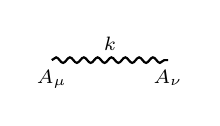
\begin{tikzpicture}[baseline=-0.6ex,scale=0.82]
  \draw[thick,decorate,decoration={snake,amplitude=1.0pt,segment length=5pt}]
    (0,0) -- (1.8,0);
  \node[above] at (0.9,0) {\scriptsize \(k\)};
  \node[below] at (0,0) {\scriptsize \(A_\mu\)};
  \node[below] at (1.8,0) {\scriptsize \(A_\nu\)};
\end{tikzpicture}
\quad
=
\frac{-\ii}{k^2-\ii\epsilon}
\left[
  \eta_{\mu\nu}
  -(1-\xi_{\mathrm g})\frac{k_\mu k_\nu}{k^2-\ii\epsilon}
\right].
\]
The cubic vertex with one photon representative and two spinor
representatives is
\[
\begin{tikzpicture}[baseline=-0.5ex,scale=0.82]
  \coordinate (v) at (0,0);
  \draw[thick,decorate,decoration={snake,amplitude=1.0pt,segment length=5pt}]
    (-1.0,0) -- (v);
  \draw[thick,-{Stealth[length=3pt]}] (v) -- (0.85,0.62);
  \draw[thick,-{Stealth[length=3pt]}] (0.85,-0.62) -- (v);
  \fill (v) circle (1.7pt);
  \node[left] at (-1.0,0) {\scriptsize \(\mu\)};
  \node[right] at (0.85,0.62) {\scriptsize \(\beta\)};
  \node[right] at (0.85,-0.62) {\scriptsize \(\alpha\)};
\end{tikzpicture}
\quad
=
-g(\gamma^\mu)_\beta{}^\alpha .
\]
For the electron convention \(g=-e\), the vertex factor is
\(e(\gamma^\mu)_\beta{}^\alpha\). The gauge parameter
\(\xi_{\mathrm g}\) appears only in the representative photon propagator.
Amplitudes between physical photon helicity states are obtained after LSZ
projection and are independent of the longitudinal representative.

\section{External Factors as Pole Data}

External factors in a diagrammatic amplitude are residues of poles already
identified by LSZ. The particle definitions have already been supplied by the
one-particle spectral data and scattering construction. With the normalizations
of Chapters 13, 16, and 18, the factors are
\[
\begin{array}{c|c}
\text{external state} & \text{LSZ factor} \\ \hline
e^-_{\mathrm{out}}(\vec p,\sigma)
&
\displaystyle
\frac{Z_\psi^{1/2}}{(2\pi)^{3/2}}\,
(\bar u^\sigma)^\alpha(\vec p)
\\[1.1em]
e^+_{\mathrm{out}}(\vec p,\sigma)
&
\displaystyle
\frac{Z_\psi^{1/2}}{(2\pi)^{3/2}}\,
v^\sigma_\alpha(\vec p)
\\[1.1em]
\gamma_{\mathrm{out}}(\vec k,h)
&
\displaystyle
\frac{Z_A^{1/2}}{(2\pi)^{3/2}\sqrt{2|\vec k|}}\,
e_\mu^{h*}(\vec k)
\\[1.1em]
e^-_{\mathrm{in}}(\vec p,\sigma)
&
\displaystyle
\frac{Z_\psi^{1/2}}{(2\pi)^{3/2}}\,
u^\sigma_\alpha(\vec p)
\\[1.1em]
e^+_{\mathrm{in}}(\vec p,\sigma)
&
\displaystyle
\frac{Z_\psi^{1/2}}{(2\pi)^{3/2}}\,
(\bar v^\sigma)^\alpha(\vec p)
\\[1.1em]
\gamma_{\mathrm{in}}(\vec k,h)
&
\displaystyle
\frac{Z_A^{1/2}}{(2\pi)^{3/2}\sqrt{2|\vec k|}}\,
e_\mu^h(\vec k).
\end{array}
\]
The free spinor or photon line adjacent to the external leg is not retained:
the LSZ operator removes that propagator and evaluates the residue at the
one-particle pole. The displayed spinor index is contracted with the
corresponding open index of the amputated Green-function kernel. In a
Fourier convention in which all momenta flow into a Green function, outgoing
massive particles are represented by the boundary value with the opposite
energy sign; the table above is written directly in terms of the physical
future-directed external momenta.

The massive spinor momenta satisfy
\[
  p^0=\omega_{\vec p}=\sqrt{\vec p^{\,2}+m^2},
\]
and the photon momentum satisfies
\[
  k^0=|\vec k|,\qquad k^2=0 .
\]
The spinors obey
\[
  (\not p-\ii m)u^\sigma(\vec p)=0,\qquad
  (\not p+\ii m)v^\sigma(\vec p)=0,
\]
with the corresponding adjoint equations for \(\bar u,\bar v\). The photon
polarization representatives obey
\[
  k^\mu e_\mu^h(\vec k)=0,\qquad
  e_\mu^h(\vec k)\sim e_\mu^h(\vec k)+\alpha k_\mu .
\]
For any polarization representative,
\[
  \not e^{\,h}(\vec k)=e_\mu^h(\vec k)\gamma^\mu .
\]

\begin{center}
\begin{tikzpicture}[>=Stealth,x=1cm,y=1cm]
  \tikzset{
    flowbox/.style={
      draw,
      rounded corners=2pt,
      align=center,
      font=\scriptsize,
      minimum height=0.72cm,
      text width=2.25cm
    },
    flowlabel/.style={font=\scriptsize,fill=white,inner sep=1.2pt}
  }
  \node[flowbox] (green) at (0,0) {gauge-fixed\\Green functions};
  \node[flowbox] (poles) at (3.35,0) {one-particle\\poles};
  \node[flowbox] (hard) at (6.7,0) {hard\\amplitude};
  \draw[->,thick] (green) -- node[flowlabel,above] {LSZ} (poles);
  \draw[->,thick] (poles) -- node[flowlabel,above] {residues} (hard);
  \draw[red!70!black,thick] (8.25,-0.72) -- (8.25,0.72);
  \node[red!70!black,align=center] at (9.35,0)
    {\scriptsize infrared\\[-0.1em]\scriptsize completion};
\end{tikzpicture}
\end{center}

The vertical mark in the diagram indicates a boundary of this chapter. The
hard-amplitude rules are perturbative rules for fixed external momenta and
helicities. The infrared completion of charged scattering is a further
construction.

Diagrammatically, the external factors attach to amputated kernels as follows:
\[
\begin{array}{cc}
\begin{tikzpicture}[baseline=(current bounding box.center),>=Stealth,scale=0.86]
  \tikzset{
    fermion/.style={line width=0.55pt,-{Stealth[length=3pt]}},
    blob/.style={circle,draw,fill=gray!16,minimum size=0.72cm,inner sep=0pt}
  }
  \node[blob] (b) at (1.25,0) {};
  \draw[fermion] (0,0)--(b);
  \node[below] at (0.62,-0.05) {\scriptsize \(u_\alpha^\sigma(\vec p)\)};
\end{tikzpicture}
&
\begin{tikzpicture}[baseline=(current bounding box.center),>=Stealth,scale=0.86]
  \tikzset{
    fermion/.style={line width=0.55pt,-{Stealth[length=3pt]}},
    blob/.style={circle,draw,fill=gray!16,minimum size=0.72cm,inner sep=0pt}
  }
  \node[blob] (b) at (0,0) {};
  \draw[fermion] (b)--(1.25,0);
  \node[below] at (0.85,-0.05) {\scriptsize \((\bar u^\sigma)^\alpha(\vec p)\)};
\end{tikzpicture}
\\[1.5em]
\begin{tikzpicture}[baseline=(current bounding box.center),>=Stealth,scale=0.86]
  \tikzset{
    photon/.style={decorate,decoration={snake,amplitude=1.1pt,segment length=5pt},line width=0.55pt},
    blob/.style={circle,draw,fill=gray!16,minimum size=0.72cm,inner sep=0pt}
  }
  \node[blob] (b) at (1.25,0) {};
  \draw[photon] (0,0)--(b);
  \node[below] at (0.55,-0.05) {\scriptsize \(e_\mu^h(\vec k)\)};
\end{tikzpicture}
&
\begin{tikzpicture}[baseline=(current bounding box.center),>=Stealth,scale=0.86]
  \tikzset{
    photon/.style={decorate,decoration={snake,amplitude=1.1pt,segment length=5pt},line width=0.55pt},
    blob/.style={circle,draw,fill=gray!16,minimum size=0.72cm,inner sep=0pt}
  }
  \node[blob] (b) at (0,0) {};
  \draw[photon] (b)--(1.25,0);
  \node[below] at (0.82,-0.05) {\scriptsize \(e_\mu^{h*}(\vec k)\)};
\end{tikzpicture}
\end{array}
\]
with the common normalization factors displayed in the table.

\section{Compton Scattering at Tree Level}

Consider the process
\[
  e^-(p,\sigma)+\gamma(k,h)
  \longrightarrow
  e^-(p',\sigma')+\gamma(k',h')
\]
with
\[
  p+k=p'+k' .
\]
At tree level two diagrams contribute:
\[
\begin{tikzpicture}[scale=0.93,baseline=(current bounding box.center)]
  \tikzset{
    photon/.style={decorate,decoration={snake,amplitude=1.1pt,segment length=5pt},line width=0.58pt}
  }
  \begin{scope}
    \draw[thick,-{Stealth[length=3pt]}] (0,0) -- (1.25,0) -- (2.5,0);
    \draw[photon,-{Stealth[length=3pt]}] (0.55,1.0) -- (0.98,0.08);
    \draw[photon,-{Stealth[length=3pt]}] (1.52,0.08) -- (1.95,1.0);
    \node[below] at (0,0) {\scriptsize \(p\)};
    \node[below] at (1.25,0) {\scriptsize \(p+k\)};
    \node[below] at (2.5,0) {\scriptsize \(p'\)};
    \node[above] at (0.52,1.0) {\scriptsize \(k\)};
    \node[above] at (2.0,1.0) {\scriptsize \(k'\)};
  \end{scope}
  \node at (3.05,0.22) {\Large \(+\)};
  \begin{scope}[xshift=3.75cm]
    \draw[thick,-{Stealth[length=3pt]}] (0,0) -- (1.25,0) -- (2.5,0);
    \draw[photon,-{Stealth[length=3pt]}] (0.55,1.0) -- (0.98,0.08);
    \draw[photon,-{Stealth[length=3pt]}] (1.52,0.08) -- (1.95,1.0);
    \node[below] at (0,0) {\scriptsize \(p\)};
    \node[below] at (1.25,0) {\scriptsize \(p-k'\)};
    \node[below] at (2.5,0) {\scriptsize \(p'\)};
    \node[above] at (0.52,1.0) {\scriptsize \(k'\)};
    \node[above] at (2.0,1.0) {\scriptsize \(k\)};
  \end{scope}
\end{tikzpicture}
\]
After removing the factor
\[
  (2\pi)^4\delta^4(p+k-p'-k')
\]
from the scattering matrix element, the reduced amplitude is
\[
\begin{aligned}
  \ii\mathcal M
  &=
  \frac{-\ii e^2}
       {(2\pi)^6\sqrt{2|\vec k|}\sqrt{2|\vec k'|}}\,
  \bar u^{\sigma'}(\vec p')
  \Biggl[
    \not e^{\,h'*}(\vec k')\,
    \frac{-\ii(\not p+\not k)+m}
         {(p+k)^2+m^2-\ii\epsilon}\,
    \not e^{\,h}(\vec k)  \\
  &\hspace{8.7em}
    +
    \not e^{\,h}(\vec k)\,
    \frac{-\ii(\not p-\not k')+m}
         {(p-k')^2+m^2-\ii\epsilon}\,
    \not e^{\,h'*}(\vec k')
  \Biggr]
  u^\sigma(\vec p).
\end{aligned}
\]
This is an LSZ-reduced expression: the external spinors and polarization
vectors are the pole residues listed above.

The expression descends from photon representatives to photon helicity states.
Let
\[
  N(q)=-\ii\not q+m,\qquad D(q)=q^2+m^2-\ii\epsilon .
\]
If the incoming polarization is shifted by
\[
  e_\mu^h(k)\mapsto e_\mu^h(k)+\alpha k_\mu ,
\]
then the first diagram changes by a factor proportional to
\[
  \frac{N(p+k)\not k}{D(p+k)}u^\sigma(p).
\]
Using \(p^2=-m^2\), \(k^2=0\), and
\((\not p-\ii m)u^\sigma(p)=0\), one obtains
\[
  N(p+k)\not k\,u^\sigma(p)
  =
  -2\ii(p\cdot k)u^\sigma(p),
  \qquad
  D(p+k)=2p\cdot k-\ii\epsilon .
\]
Thus the first diagram contributes
\[
  -\ii\alpha\,
  \bar u^{\sigma'}(p')\not e^{\,h'*}(k')u^\sigma(p)
\]
up to the common prefactor. For the second diagram, momentum conservation
gives \(p-k'=p'-k\), and the adjoint Dirac equation gives
\[
  \bar u^{\sigma'}(p')\not k\,N(p-k')
  =
  -2\ii(p'\cdot k)\bar u^{\sigma'}(p'),
  \qquad
  D(p-k')=-2p'\cdot k-\ii\epsilon .
\]
The second diagram therefore contributes
\[
  +\ii\alpha\,
  \bar u^{\sigma'}(p')\not e^{\,h'*}(k')u^\sigma(p)
\]
with the same common prefactor. The two shifts cancel. The same argument
applies to shifts of the outgoing photon representative. This cancellation is
the tree-level Ward identity for the Compton amplitude.

With the cross-section normalization of
Chapter~\ref{ch:cross-sections-unitarity}, the total cross section
for fixed incoming spin and helicity is
\[
\begin{aligned}
  \sigma
  &=
  \frac{(2\pi)^6}{v}
  \int\dd^3\vec k'\,\dd^3\vec p'\,
  (2\pi)^4\delta^4(k+p-k'-p')  \\
  &\qquad\times
  \sum_{\substack{h'=\pm1\\ \sigma'=1,2}}
  \left|
    \mathcal M(\vec p',\sigma';\vec k',h'
    \mid
    \vec p,\sigma;\vec k,h)
  \right|^2 ,
\end{aligned}
\]
where \(v\) is the incoming relative velocity. The evaluation of the spin
and polarization sums is a kinematic exercise built from the completeness
relations of Chapters 16 and 17.

\section{Infrared Boundary of Charged Scattering}

The perturbative rules above are rules for hard Green-function residues. They
are valid order by order once an infrared regulator or an inclusive
prescription has been specified. The exact long-range theory has an additional
structural feature: Gauss' law ties electric charge to an electromagnetic
field extending to arbitrarily large distances. Consequently the charged-sector
asymptotic data is infrared-sensitive: its spectral support is tied to the
charged mass threshold together with arbitrarily soft radiation. This lies
outside the isolated massive-particle hypothesis used in the basic
Haag--Ruelle construction.

This boundary is already visible in the charged dressing
\(\Psi_{C_x}(x)\). A dressing that retains nonzero electric charge extends to
infinity. In scattering, the same long-range field is represented
perturbatively by arbitrarily soft photons.
The physical completions are inclusive transition probabilities, where soft
photons below a resolution threshold are summed over, or dressed asymptotic
charged states. Those constructions belong after renormalization and the
analysis of infrared singularities. The present chapter supplies the
gauge-fixed hard-amplitude rules on which that later analysis acts.

\chapter{QED Renormalization and Electromagnetic Form Factors}
\label{ch:qed-renormalization-form-factors}
\ConventionsLorentzian


\section{Bare Variables and Ward Organization}

Use the electron convention of Chapter~\ref{ch:qed-external-states}. The bare
representative fields and
parameters are
\[
  A_\mu^B,\qquad \psi^B,\qquad \bar\psi^B,\qquad m^B,\qquad e^B,
\]
and the bare Lagrangian is
\[
  \mathcal L_B
  =
  -\frac14F^B_{\mu\nu}F_B^{\mu\nu}
  -
  \bar\psi^B
  \left[
    \gamma^\mu(\partial_\mu+\ii e^B A_\mu^B)+m^B
  \right]\psi^B .
\]
This is the explicit-coupling QED normalization: the photon representative has
a canonical kinetic term, and the electric charge appears in the covariant
derivative.  It differs from the coupling-absorbed Yang--Mills normalization of
Chapter~\ref{ch:vol2-classical-yang-mills-matter}.  In the notation of
\eqref{eq:ym-qed-curvature-rescaling}, the electron convention \(g=-e\) gives
\(A_\mu^{\rm YM}=-eA_\mu^{\rm QED}\) and
\(F_{\mu\nu}^{\rm YM}=-eF_{\mu\nu}^{\rm QED}\).  Therefore the photon
renormalization constant \(Z_A\) below is a field-residue constant in
explicit-coupling coordinates; after the rescaling to Yang--Mills coordinates
the same running is read from the coefficient of
\((F_{\mu\nu}^{\rm YM})^2/e^2\).
Introduce renormalized representative fields by
\[
  A_\mu^B=Z_A^{1/2}A_\mu,\qquad
  \psi^B=Z_\psi^{1/2}\psi,\qquad
  \bar\psi^B=Z_\psi^{1/2}\bar\psi .
\]
The constants \(Z_A\) and \(Z_\psi\) are fixed by pole-residue
normalizations in the infrared-regulated hard theory: \(Z_A\) normalizes the
one-photon component of \(\widehat F_{\mu\nu}\ket{\vac}\), and \(Z_\psi\)
normalizes the one-electron and one-positron spinor poles before the
long-distance regulator is removed.  In exact massless QED, \(Z_\psi\) is not
a physical residue of an isolated electron Wigner particle; its infrared
dependence is part of the hard-kernel bookkeeping that is combined with soft
radiation in Chapter~\ref{ch:volume-ii-infrared-inclusive-qed}. Write
\[
  m^B=m+\delta m .
\]

The renormalized charge parameter \(e\) is fixed by the electromagnetic
current matrix element at zero momentum transfer. Gauge covariance of the
renormalized representative derivative requires
\[
  e=e^B Z_A^{1/2},
\]
so that
\[
  \partial_\mu+\ii e^B A_\mu^B
  =
  \partial_\mu+\ii e A_\mu .
\]
Equivalently, if a separate vertex constant \(Z_1\) is introduced by
\[
  e^B Z_A^{1/2}Z_\psi=eZ_1,
\]
then Abelian gauge covariance gives the Ward organization
\[
  Z_1=Z_\psi .
\]
The same statement can be read from the renormalized representative gauge
transformation,
\[
  A_\mu\mapsto A_\mu+\partial_\mu\xi,\qquad
  \psi\mapsto \ee^{-\ii e\xi}\psi,\qquad
  \bar\psi\mapsto \bar\psi\,\ee^{\ii e\xi}.
\]
The coefficient \(e\), not \(eZ_\psi\), is the charge appearing in this
transformation law.  The common factor \(Z_\psi\) multiplies the whole spinor
covariant derivative and therefore belongs to the spinor residue
normalization.
Thus
\[
  \mathcal L_B
  =
  -\frac14Z_A F_{\mu\nu}F^{\mu\nu}
  -
  Z_\psi\bar\psi
  \left[
    \gamma^\mu(\partial_\mu+\ii e A_\mu)+m+\delta m
  \right]\psi .
\]
Split this into a renormalized quadratic and interaction part plus
counterterms:
\[
\begin{aligned}
  \mathcal L_B
  &=
  \underbrace{
    -\frac14F_{\mu\nu}F^{\mu\nu}
    -\bar\psi(\gamma^\mu\partial_\mu+m)\psi
    -\ii eA_\mu\bar\psi\gamma^\mu\psi
  }_{\mathcal L_{\mathrm{ren}}}
\\
  &\quad
  -\frac14(Z_A-1)F_{\mu\nu}F^{\mu\nu}
  -(Z_\psi-1)\bar\psi(\gamma^\mu\partial_\mu+m)\psi
  -Z_\psi\delta m\,\bar\psi\psi
\\
  &\quad
  -\ii e(Z_\psi-1)A_\mu\bar\psi\gamma^\mu\psi .
\end{aligned}
\]
The last line is the vertex counterterm tied to the spinor wavefunction
counterterm by the Abelian Ward identity. The mass counterterm is independent
because \(m\bar\psi\psi\) is gauge-invariant.

The current normalized by the renormalized field strength is obtained from
the Euler--Lagrange equation for \(A_\mu\):
\[
  \partial_\nu F^{\mu\nu}
  =
  -\ii Z_A^{-1}eZ_\psi\,\bar\psi\gamma^\mu\psi
  \equiv j^\mu .
\]
This identity is an operator identity at separated insertions in the regulated
theory.  In time-ordered products, differentiating the ordering symbols may
also produce local contact terms; the nonlocal momentum dependence discussed
below is insensitive to such polynomial contact terms.

\section{Photon Self-Energy and Transversality}

Let
\[
  \bra{\vac}
  \operatorname T\{\widehat A_\mu(x)\widehat A_\nu(0)\}
  \ket{\vac}
  =
  \int\frac{\dd^4k}{(2\pi)^4}\,
  \ee^{\ii k\cdot x}\,\widetilde G_{\mu\nu}(k).
\]
The full photon representative two-point function is obtained by inserting
one-particle-irreducible photon self-energies into the free propagator:
\[
\begin{gathered}
\begin{tikzpicture}[baseline=(current bounding box.center),>=Stealth,scale=0.88]
  \tikzset{
    photon/.style={decorate,decoration={snake,amplitude=1.15pt,segment length=5pt},line width=0.55pt}
  }
  \draw[photon] (-0.2,0)--(1.0,0);
  \node at (1.45,0) {\(=\)};
  \draw[photon] (1.9,0)--(3.1,0);
  \node at (3.55,0) {\(+\)};
  \draw[photon] (4.05,0)--(4.75,0);
  \node[circle,draw,minimum size=0.48cm,inner sep=0pt] at (5.05,0) {\scriptsize 1PI};
  \draw[photon] (5.35,0)--(6.05,0);
  \node at (6.5,0) {\(+\)};
  \draw[photon] (7.0,0)--(7.55,0);
  \node[circle,draw,minimum size=0.45cm,inner sep=0pt] at (7.82,0) {\scriptsize 1PI};
  \draw[photon] (8.1,0)--(8.65,0);
  \node[circle,draw,minimum size=0.45cm,inner sep=0pt] at (8.92,0) {\scriptsize 1PI};
  \draw[photon] (9.2,0)--(9.75,0);
  \node at (10.25,0) {\(\cdots\)};
\end{tikzpicture}
\end{gathered}
\]
Let \(\ii\Pi^{\mu\nu}(k)\) denote the sum of amputated one-particle
irreducible photon two-point insertions.  Current conservation implies
transversality in a way that does not depend on a gauge-dependent
longitudinal representative.  The Maxwell equation with the renormalized
current has the form
\[
  \partial_\nu \widehat F^{\mu\nu}=\widehat j^\mu,
  \qquad
  \partial_\mu\widehat j^\mu=0
\]
at separated points.  Let \(M^{\mu\nu}(k)\) be the noncontact coefficient in
the Fourier transform of
\(\bra{\vac}\operatorname T\widehat j^\mu(x)\widehat j^\nu(0)\ket{\vac}\).
Then
\[
  k_\mu M^{\mu\nu}(k)=0,\qquad k_\nu M^{\mu\nu}(k)=0 .
\]
On the other hand, applying
\(\partial_\alpha F^{\mu\alpha}\) to the photon Dyson series acts on each
external photon line by the transverse differential operator
\[
  k^2\eta^{\mu\rho}-k^\mu k^\rho .
\]
The local contact terms are polynomials in \(k\).  The nonlocal part is
therefore transverse only if the amputated 1PI insertion obeys
\[
  k_\mu\Pi^{\mu\nu}(k)=0 .
\]
Lorentz covariance then gives the tensor decomposition
\[
  \Pi^{\mu\nu}(k)
  =
  (\eta^{\mu\nu}k^2-k^\mu k^\nu)\pi(k^2)
\]
for a scalar function \(\pi\).

In covariant gauge, with gauge parameter \(\xi_{\mathrm g}\), the resummed
propagator is
\[
  \widetilde G_{\mu\nu}(k)
  =
  \frac{-\ii}{k^2-\ii\epsilon}
  \left[
    \frac{\eta_{\mu\nu}}{1-\pi(k^2)}
    -
    \frac{k_\mu k_\nu}{k^2-\ii\epsilon}
    \left(
      1-\xi_{\mathrm g}
      +\frac{\pi(k^2)}{1-\pi(k^2)}
    \right)
  \right].
\]
The longitudinal part depends on the representative gauge choice. The
transverse pole is normalized by imposing
\[
  \pi(0)=0
\]
for the massive-electron theory, where the loop function is regular at the
photon point \(k^2=0\).

\section{One-Loop Vacuum Polarization}

The photon counterterm contributes
\[
\begin{tikzpicture}[baseline=(current bounding box.center),>=Stealth,scale=0.82]
  \tikzset{photon/.style={decorate,decoration={snake,amplitude=1.1pt,segment length=5pt},line width=0.55pt}}
  \draw[photon] (-1.25,0)--(1.25,0);
  \draw[thick] (0,-0.18)--(0,0.18);
  \node[below] at (-1.25,-0.08) {\scriptsize \(\mu\)};
  \node[below] at (1.25,-0.08) {\scriptsize \(\nu\)};
\end{tikzpicture}
\quad
=
-\ii(Z_A-1)(k^2\eta_{\mu\nu}-k_\mu k_\nu),
\]
which contributes \(1-Z_A\) to \(\pi(k^2)\). The one-loop electron diagram is
\[
\begin{tikzpicture}[baseline=(current bounding box.center),>=Stealth,scale=0.9]
  \tikzset{
    photon/.style={decorate,decoration={snake,amplitude=1.1pt,segment length=5pt},line width=0.55pt},
    fermion/.style={postaction={decorate,decoration={markings,mark=at position .58 with {\arrow{Stealth}}}},line width=0.55pt}
  }
  \draw[photon] (-1.7,0)--(-0.62,0);
  \draw[fermion] (0,0) circle (0.62);
  \draw[photon] (0.62,0)--(1.7,0);
  \node[below] at (-1.7,-0.08) {\scriptsize \(\mu\)};
  \node[below] at (1.7,-0.08) {\scriptsize \(\nu\)};
  \node[above] at (0,0.70) {\scriptsize \(p\)};
  \node[below] at (0,-0.72) {\scriptsize \(p-k\)};
\end{tikzpicture}
\]
and equals
\[
\begin{aligned}
  \ii\Pi^{(1)}_{\mu\nu}(k)
  &=
  -
  \int\frac{\dd^4p}{(2\pi)^4}
  \operatorname{Tr}\left[
    e\gamma_\mu\,
    \frac{-\ii(-\ii\not p+m)}{p^2+m^2-\ii\epsilon}\,
    e\gamma_\nu\,
    \frac{-\ii(-\ii(\not p-\not k)+m)}
         {(p-k)^2+m^2-\ii\epsilon}
  \right].
\end{aligned}
\]
The minus sign is the closed fermion loop. Continue the integral to
\(D=4-\epsilon\) dimensions, keeping
\[
  \{\gamma_\mu,\gamma_\nu\}=2\eta_{\mu\nu},\qquad
  \eta^{\mu\nu}\eta_{\mu\nu}=D,\qquad
  \operatorname{Tr}\mathbf 1=4 .
\]
After Wick rotation and the Feynman-parameter identity
\[
  \frac1{ab}=\int_0^1\dd x\,
  \frac1{\bigl(xa+(1-x)b\bigr)^2},
\]
shift
\[
  p\mapsto p+xk .
\]
The denominator becomes
\[
  \bigl(p^2+x(1-x)k^2+m^2\bigr)^2 .
\]
The trace identity
\[
  \operatorname{Tr}(
    \gamma_\mu\gamma_\alpha\gamma_\nu\gamma_\beta)
  =
  4(
    \eta_{\mu\alpha}\eta_{\nu\beta}
    -\eta_{\mu\nu}\eta_{\alpha\beta}
    +\eta_{\mu\beta}\eta_{\nu\alpha})
\]
reduces the numerator. Rotational symmetry in the continued loop momentum
allows
\[
  p_\mu p_\nu\mapsto \frac1D\eta_{\mu\nu}p^2
\]
inside the integral, and all terms linear in \(p\) vanish.  With
\[
  M_x^2=m^2+x(1-x)k^2,
\]
the angularly averaged numerator can be written as
\[
\begin{aligned}
  N_{\mu\nu}
  =
  4\Bigl[
    &\eta_{\mu\nu}\bigl(p^2-x(1-x)k^2+m^2\bigr)
    -\frac2D\eta_{\mu\nu}p^2
\\
    &\qquad\qquad
    +2x(1-x)k_\mu k_\nu
  \Bigr].
\end{aligned}
\]
The two scalar integrals needed are
\[
\begin{aligned}
  \int\frac{\dd^Dp}{(2\pi)^D}\frac1{(p^2+M_x^2)^2}
  &=
  \frac1{(4\pi)^{D/2}}
  \Gamma(2-D/2)(M_x^2)^{D/2-2},\\
  \int\frac{\dd^Dp}{(2\pi)^D}\frac{p^2}{(p^2+M_x^2)^2}
  &=
  \frac{D}{2}\frac1{(4\pi)^{D/2}}
  \Gamma(1-D/2)(M_x^2)^{D/2-1},
\end{aligned}
\]
where the second formula is defined by analytic continuation in \(D\).
Substitution cancels the nontransverse local-looking pieces and leaves the
transverse tensor
\[
  \Pi^{(1)}_{\mu\nu}(k)
  =
  -(\eta_{\mu\nu}k^2-k_\mu k_\nu)
  \frac{8e^2}{(4\pi)^{D/2}}
  \Gamma(2-D/2)
  \int_0^1\dd x\,x(1-x)
  \bigl(m^2+x(1-x)k^2\bigr)^{D/2-2}.
\]
With the counterterm included,
\[
  \pi(k^2)
  =
  1-Z_A
  -
  \frac{8e^2}{(4\pi)^{D/2}}\Gamma(2-D/2)
  \int_0^1\dd x\,x(1-x)
  \bigl(m^2+x(1-x)k^2\bigr)^{D/2-2}.
\]
The pole normalization \(\pi(0)=0\) fixes
\[
  Z_A
  =
  1-
  \frac{8e^2}{(4\pi)^{D/2}}\Gamma(2-D/2)\frac16\,m^{D-4}.
\]
For \(D=4-\epsilon\), this has the pole part
\[
  Z_A=1-\frac{e^2}{6\pi^2}\frac1\epsilon+\text{finite}.
\]
Subtracting the value at \(k^2=0\) and taking \(D\to4\) gives the finite
one-loop vacuum-polarization function
\[
  \pi(k^2)
  =
  \frac{e^2}{2\pi^2}
  \int_0^1\dd x\,x(1-x)
  \log
  \frac{m^2+x(1-x)k^2}{m^2}.
\]
This \(\pi(k^2)\) is the cutoff-removed form factor: in a cutoff
realization it is the \(\Lambda\to\infty\) limit of the renormalized
transverse coefficient in the photon two-point matrix element, with the
charge normalization \(\pi(0)=0\) held fixed.  In dimensional
regularization the same statement is represented by the analytic continuation
to \(D=4\) after the local counterterm \(Z_A\) has subtracted the ultraviolet
pole.

\section{The Electron Current Matrix Element}

Let \(|\vec p,\sigma\rangle\) be a one-electron state of charge \(q=-e\).
Translation covariance gives
\[
  \langle\vec p',\sigma'|\widehat j^\mu(x)|\vec p,\sigma\rangle
  =
  \ee^{\ii(p-p')\cdot x}
  \langle\vec p',\sigma'|\widehat j^\mu(0)|\vec p,\sigma\rangle .
\]
Write the matrix element as
\[
  \langle\vec p',\sigma'|\widehat j^\mu(0)|\vec p,\sigma\rangle
  =
  \frac{\ii q}{(2\pi)^3}
  \bar u^{\sigma'}(\vec p')M^\mu(p',p)u^\sigma(\vec p).
\]
Modulo the on-shell Dirac equations
\[
  (\not p-\ii m)u^\sigma(\vec p)=0,\qquad
  \bar u^{\sigma'}(\vec p')(\not p'-\ii m)=0,
\]
a parity-even Lorentz vector between spinor solutions can be reduced, by the
Clifford algebra, to the span of
\[
  \gamma^\mu,\qquad (p+p')^\mu,\qquad (p-p')^\mu .
\]
Terms with \(\gamma_5\) are excluded by parity, and terms with
\([\gamma^\mu,\gamma^\nu]\) are equivalent to the displayed basis by the
Gordon identity.  Current conservation removes the component proportional to
\((p-p')^\mu\). Therefore
\[
  M^\mu(p',p)
  =
  \gamma^\mu F(k^2)
  -\frac{\ii}{2m}(p+p')^\mu G(k^2),
  \qquad
  k=p-p' .
\]
The scalar functions \(F\) and \(G\) are the electromagnetic form factors in
the present gamma-matrix convention and in the \((p+p')^\mu\) basis.  For
comparison with the Dirac--Pauli basis, let
\(F_1^{\rm DP}\) and \(F_2^{\rm DP}\) be defined in this same gamma-matrix
convention by
\[
  \bar u(p')M^\mu u(p)
  =
  \bar u(p')
  \left[
    \gamma^\mu F_1^{\rm DP}(k^2)
    +
    \left(\gamma^\mu+\frac{\ii}{2m}(p+p')^\mu\right)
    F_2^{\rm DP}(k^2)
  \right]
  u(p).
\]
The second structure is the Gordon-identity form of the Pauli tensor
structure; its matrix element vanishes at \(p'=p\).  Comparing coefficients
with the displayed \((F,G)\) decomposition gives
\[
  F_1^{\rm DP}=F+G,
  \qquad
  F_2^{\rm DP}=-G,
  \qquad
  F=F_1^{\rm DP}+F_2^{\rm DP}.
\]
Thus the charge normalization below, \(F(0)+G(0)=1\), is precisely
\(F_1^{\rm DP}(0)=1\), while the anomalous magnetic moment is
\(F_2^{\rm DP}(0)=-G(0)\).

Charge normalization fixes one combination at zero momentum transfer. Taking
\(p'\to p\), using
\[
  \bar u^{\sigma'}(\vec p)u^\sigma(\vec p)
  =
  \frac{m}{p^0}\delta_{\sigma\sigma'},
\]
and using the Dirac equations to rewrite
\[
  p^\mu\bar u^{\sigma'}(\vec p)u^\sigma(\vec p)
  =
  \ii m\,\bar u^{\sigma'}(\vec p)\gamma^\mu u^\sigma(\vec p),
\]
one obtains
\[
  \langle\vec p,\sigma'|\widehat j^\mu(0)|\vec p,\sigma\rangle
  =
  \frac{q}{(2\pi)^3}
  \frac{p^\mu}{p^0}
  \delta_{\sigma\sigma'}\bigl(F(0)+G(0)\bigr).
\]
The charge operator
\[
  \widehat Q=\int\dd^3\vec x\,\widehat j^0(x)
\]
acts by
\[
  \widehat Q|\vec p,\sigma\rangle=q|\vec p,\sigma\rangle .
\]
Thus
\[
  F(0)+G(0)=1.
\]
The equality is a distributional momentum-state identity: after smearing the
external plane waves by a common wave packet and then removing the smearing,
the spatial integral supplies the same
\(\delta^{(3)}(\vec p'-\vec p)\) on both sides.

\section{Magnetic Moment from the Form Factor}

Couple the current to a weak classical background:
\[
  \Delta H
  =
  -\int\dd^3\vec x\,A_\mu^{\mathrm{cl}}(x)\widehat j^\mu(x).
\]
For a slowly varying magnetic field choose
\[
  A_0^{\mathrm{cl}}=0,\qquad
  \nabla\times\vec A^{\mathrm{cl}}=\vec B .
\]
The part of the form-factor matrix element proportional to
\((p+p')^\mu\) gives the spin-independent Lorentz-force contribution in the
nonrelativistic limit.  The spin-dependent term is exposed by writing the
\(\gamma^\mu F\) term with the Gordon identity.  Equivalently, after an
integration by parts,
\[
  \int\dd^3\vec x\,
  A_i^{\mathrm{cl}}(x)\,
  \ee^{\ii(\vec p-\vec p')\cdot\vec x}(p'-p)_jS^{ij}
  =
  \frac{\ii}{2}\int\dd^3\vec x\,
  \ee^{\ii(\vec p-\vec p')\cdot\vec x}
  F^{\mathrm{cl}}_{ij}(x)S^{ij},
\]
up to terms higher order in the spatial momentum transfer; only the
antisymmetric part contributes to the spin coupling.
The spin-dependent part of
\(\langle\vec p',\sigma'|\Delta H|\vec p,\sigma\rangle\) is obtained from
the identity
\[
\begin{aligned}
  &\bar u^{\sigma'}(\vec p')
  [\gamma^\mu,\gamma^\nu](p'-p)_\nu
  u^\sigma(\vec p)  \\
  &\quad =
  -4\ii m\,\bar u^{\sigma'}(\vec p')\gamma^\mu u^\sigma(\vec p)
  +2(p^\mu+p'^\mu)
  \bar u^{\sigma'}(\vec p')u^\sigma(\vec p),
\end{aligned}
\]
with
\[
  S^{\mu\nu}=-\frac{\ii}{4}[\gamma^\mu,\gamma^\nu].
\]
In the nonrelativistic limit \(|\vec p|,|\vec p'|\ll m\), the spin
coupling becomes
\[
  \Delta H_{\mathrm{spin}}
  =
  -\frac{qF(0)}{2m}\,\vec B\cdot\vec\sigma .
\]
Writing this as
\[
  \Delta H_{\mathrm{spin}}
  =
  -g_{\mathrm{mag}}\frac{q}{2m}\,
  \vec B\cdot\frac{\vec\sigma}{2},
\]
the magnetic factor is
\[
  g_{\mathrm{mag}}=2F(0).
\]
Together with \(F(0)+G(0)=1\), this gives
\[
  g_{\mathrm{mag}}=2\bigl(1-G(0)\bigr).
\]

\section{One-Loop Vertex Correction}

The current is represented by
\[
  \widehat j^\mu
  =
  -\ii Z_A^{-1}e\,Z_\psi\,\bar\psi\gamma^\mu\psi
  =
  -\ii e^B Z_A^{-1/2}Z_\psi\,\bar\psi\gamma^\mu\psi .
\]
Within the same infrared-regulated hard-kernel convention, the current
insertion between external electron labels is computed by reducing the
external spinor legs by LSZ:
\[
\begin{tikzpicture}[baseline=(current bounding box.center),>=Stealth,scale=0.88]
  \tikzset{
    fermion/.style={postaction={decorate,decoration={markings,mark=at position .58 with {\arrow{Stealth}}}},line width=0.55pt},
    photon/.style={decorate,decoration={snake,amplitude=1.15pt,segment length=5pt},line width=0.55pt}
  }
  \coordinate (v) at (0,0);
  \draw[fermion] (v)--(1.0,0.65);
  \draw[fermion] (1.0,-0.65)--(v);
  \draw[photon] (-0.95,0)--(v);
  \draw[fill=white,line width=0.55pt] (v) circle (0.1);
  \draw[line width=0.55pt] (-0.07,-0.07)--(0.07,0.07);
  \draw[line width=0.55pt] (-0.07,0.07)--(0.07,-0.07);
  \node[left] at (-0.95,0) {\scriptsize \(j^\mu\)};
  \node[right] at (1.05,0.65) {\scriptsize \(\bar u(p')\)};
  \node[right] at (1.05,-0.65) {\scriptsize \(u(p)\)};
\end{tikzpicture}
\]
If the three-point function is written in bare fields, each external fermion
leg supplies a factor \(Z_\psi^{1/2}\) in the LSZ residue.  If it is written
in renormalized fields, those factors are absent from the external residues
but reappear through the counterterm vertices.  These two bookkeepings give
the same matrix element.
After removing the infrared regulator in massless QED, this exclusive
one-electron matrix element is not an autonomous physical scattering
amplitude.  The hard form factor is one factor in either an inclusive
probability, where unresolved photons are summed over, or a dressed-state
matrix element whose charged asymptotic state already contains the soft
electromagnetic field.

The tree current vertex gives
\[
  -\ii Z_A^{-1}e\,\frac{Z_\psi}{(2\pi)^3}
  \bar u^{\sigma'}(\vec p')\gamma^\mu u^\sigma(\vec p).
\]
The current insertion can also be followed by any number of photon
self-energy insertions before the photon attaches to the electron line.  The
transverse photon chain contributes \(Z_A/(1-\pi(k^2))\), so the whole
tree-plus-vacuum-polarization chain contributes
\[
  -\ii e\,\frac{Z_\psi}{(2\pi)^3}
  \frac1{1-\pi(k^2)}
  \bar u^{\sigma'}(\vec p')\gamma^\mu u^\sigma(\vec p).
\]
This changes only the coefficient of \(\gamma^\mu\), hence only \(F(k^2)\).
It does not contribute to \(G(k^2)\).

At order \(e^2\), the contribution to \(G(k^2)\) comes from the vertex
correction
\[
\begin{tikzpicture}[baseline=(current bounding box.center),>=Stealth,scale=0.95]
  \tikzset{
    fermion/.style={postaction={decorate,decoration={markings,mark=at position .58 with {\arrow{Stealth}}}},line width=0.55pt},
    photon/.style={decorate,decoration={snake,amplitude=1.15pt,segment length=5pt},line width=0.55pt}
  }
  \coordinate (v) at (0,0);
  \coordinate (a) at (0.9,0.72);
  \coordinate (b) at (0.9,-0.72);
  \draw[fermion] (v)--(a);
  \draw[fermion] (b)--(v);
  \draw[photon] (a)--(b);
  \draw[fermion] (a)--(1.9,1.08);
  \draw[fermion] (1.9,-1.08)--(b);
  \draw[photon] (-0.85,0)--(v);
  \draw[fill=white,line width=0.55pt] (v) circle (0.1);
  \draw[line width=0.55pt] (-0.07,-0.07)--(0.07,0.07);
  \draw[line width=0.55pt] (-0.07,0.07)--(0.07,-0.07);
  \node[left] at (-0.85,0) {\scriptsize \(k=p-p'\)};
  \node[above] at (1.45,0.98) {\scriptsize \(p'-q\)};
  \node[below] at (1.45,-0.98) {\scriptsize \(p-q\)};
  \node[right] at (1.05,0) {\scriptsize \(q\)};
\end{tikzpicture}
\]
in Feynman gauge. Its integrand is
\[
\begin{aligned}
  &-\ii Z_A^{-1}e\,\frac{Z_\psi}{(2\pi)^3}
  \int\frac{\dd^4q}{(2\pi)^4}
  \frac{-\ii}{q^2-\ii\epsilon}\,
  \bar u(p')\,e\gamma^\rho
  \frac{-\ii[-\ii(\not p'-\not q)+m]}
       {(p'-q)^2+m^2-\ii\epsilon}
\\
  &\hspace{9em}\times
  \gamma^\mu
  \frac{-\ii[-\ii(\not p-\not q)+m]}
       {(p-q)^2+m^2-\ii\epsilon}
  e\gamma_\rho\,u(p).
\end{aligned}
\]
To isolate the term that affects the magnetic moment, Wick rotate, continue
the loop integral dimensionally, combine the three denominators by Feynman
parameters, and use the external Dirac equations.  The reduced numerator has
the form
\[
  \bar u(p')\gamma^\mu u(p)\,A(k^2)
  +(p+p')^\mu\bar u(p')u(p)\,B(k^2).
\]
The scalar \(A(k^2)\) contains ultraviolet and infrared singular terms whose
contribution is fixed by the charge normalization and the spinor
wavefunction counterterm.  The scalar \(B(k^2)\) is finite at this order and
determines \(G(k^2)\).  The resulting coefficient is
\[
  G(k^2)
  =
  -\frac{e^2m^2}{4\pi^2}
  \int_0^1\dd x\int_0^x\dd y\,
  \frac{x(1-x)}
       {m^2x^2+k^2y(x-y)} .
\]
The displayed \(G(k^2)\) is again the cutoff-removed form factor: for fixed
external on-shell wave packets and fixed nonzero momentum-transfer invariant
away from infrared singular loci, it is the ultraviolet-regulator removal
limit of the renormalized coefficient multiplying
\((p+p')^\mu\bar u(p')u(p)\) in the current matrix element.  The charge
normalization and the wavefunction counterterm determine the accompanying
\(\gamma^\mu\) coefficient, while no additional ultraviolet subtraction is
needed for this one-loop \(G(k^2)\).
At zero momentum transfer,
\[
  \int_0^1\dd x\int_0^x\dd y\,
  \frac{x(1-x)}{m^2x^2}
  =
  \frac1{2m^2},
  \qquad
  G(0)
  =
  -\frac{e^2}{8\pi^2}.
\]
With
\[
  \alpha=\frac{e^2}{4\pi},
\]
the one-loop magnetic factor is
\[
  g_{\mathrm{mag}}
  =
  2\bigl(1-G(0)\bigr)
  =
  2+\frac{\alpha}{\pi}+O(\alpha^2).
\]

